% libroResMat2
% Copyright (C) 2020  J.M. Perez Zerpa, et. al.
%
% This program is free software: you can redistribute it and/or modify
% it under the terms of the GNU General Public License as published by
% the Free Software Foundation version 3 of the License.
%
% This program is distributed in the hope that it will be useful,
% but WITHOUT ANY WARRANTY; without even the implied warranty of
% MERCHANTABILITY or FITNESS FOR A PARTICULAR PURPOSE. See the
% GNU General Public License for more details.
%
% You should have received a copy of the GNU General Public License
% along with this program.  If not, see <http://www.gnu.org/licenses/>.
%
\documentclass{textbook}

% --- fuentes e idioma ---
\usepackage[utf8]{inputenc}
\usepackage[T1]{fontenc}
\usepackage{libertine}
\usepackage{textcase}
\usepackage[spanish,es-nodecimaldot]{babel}
% ------------------------

\usepackage{libertinust1math}
\usepackage{titlesec}

\usepackage[usenames]{xcolor}
\usepackage{graphicx,epsfig}
\usepackage{mathrsfs,amsfonts,amssymb,amsmath,amsthm,mathtools}


\definecolor{bluedark}{rgb}{0,0.1,0.5}%
\definecolor{miblue}{rgb}{0,0.1,0.6}%

\usepackage[colorlinks = true,
linkcolor = miblue,
urlcolor  = miblue,
citecolor = blue,
anchorcolor = miblue]{hyperref}

\usepackage{anysize}

\usepackage{wasysym}
\usepackage{ifthen}

\usepackage{subfig}

\usepackage{natbib,apalike}

\usepackage{enumitem}

\usepackage{lipsum}
\usepackage{tcolorbox}

\tcbuselibrary{skins,breakable}
\usetikzlibrary{shadings,shadows}

\usepackage[pagewise]{lineno}

\usepackage[font=footnotesize]{caption}

% Paquetes añadidos por JVS
\usepackage{float}
\usepackage{booktabs}
\usepackage{array}

% formato 
\usepackage[paperwidth=6in,paperheight=9in,%
            top=16.5mm,bottom=12.8mm,left=15mm,right=6mm,%
            portrait]{geometry}


%\usepackage[a4,center,frame,noinfo]{crop}
\usepackage[a4,center,frame]{crop}

\setlength{\columnseprule}{.05mm}
\setlength{\columnsep}{10mm}

\usepackage{listings}
\lstset{%
  language=Octave, %
  basicstyle=\small,
  commentstyle=\color{mygreen},
  keywordstyle=\color{blue},
  morecomment = [l][\itshape\color{mygreen}]{\%},
  showspaces=false, % show spaces adding particular underscores
  showstringspaces=false, % underline spaces within strings
  frame=single % adds a frame around the code
  %breaklines=true, % sets automatic line breaking
  title=\lstname
}

\makeatletter
\def\mathcolor#1#{\@mathcolor{#1}}
\def\@mathcolor#1#2#3{%
	\protect\leavevmode
	\begingroup
	\color#1{#2}#3%
	\endgroup
}
\makeatother

% codigos embebidos
\usepackage[numbered,framed]{matlab-prettifier}

\let\ph\mlplaceholder % shorter macro
\lstMakeShortInline"

\lstset{
	style              = Matlab-editor,
	basicstyle         = \footnotesize\mlttfamily,
	language           = Octave,
	escapechar         = ",
	mlshowsectionrules = true,
}
\renewcommand\lstlistingname{Código}
% --------------------------------

% --- colores ---
\definecolor{grisecito}{rgb}{0.1,0.1,0,1}
%\definecolor{BlueLUH}{cmyk}{1.0,0.7,0.0}
\definecolor{ultramarine}{rgb}{0.07, 0.04, 0.56} 

\definecolor{mygreen}{rgb}{0,0.6,0}
\definecolor{migreen}{rgb}{0.1,0.3,0}%
\definecolor{ugentblauw}{cmyk}{1 0.8 0.3 0.05}%
\definecolor{miblue}{rgb}{0,0.1,0.6}%
\definecolor{bluedark}{rgb}{0,0.1,0.5}%
\definecolor{colorbordecajas}{rgb}{0,0.1,0.4}%
\definecolor{colorfondocajas}{rgb}{.86,.91,.996}%
\definecolor{colorbordecajasconcepto}{rgb}{0.1,0.33,0.01}%
\definecolor{colorfondocajasconcepto}{rgb}{.9,.99,.8}%
\colorlet{shadecolor}{ugentblauw}
% ---------------

\newenvironment{definicion}[1]{%
	\tcolorbox[beamer,%
	noparskip,breakable,
	colback=white,
	colframe=ultramarine,%
%	colbacklower=grisecito,%
%	colbacklower=DarkBlue!95!LightBlue,%
	colbacklower=ultramarine,%
	title=#1]}%
{\endtcolorbox}
%	colbacklower=DarkBlue!95!LightBlue,%


\newenvironment{ejemplo}[1]{%
	\tcolorbox[beamer,%
	noparskip,breakable,
	colback=LightGreen,colframe=DarkGreen,%
	colbacklower=LimeGreen!75!LightGreen,%
	title=#1]}%
{\endtcolorbox}

\newcommand{\includecode}[2][c]{\lstinputlisting[caption=#2]{#2}}
%\renewcommand{\baselinestretch}{1.15}
\renewcommand{\baselinestretch}{1.05}
%\renewcommand{\tablename}{Tabla}
\addto{\captionsspanish}{\renewcommand*{\contentsname}{Lista de contenidos}}
\addto{\captionsspanish}{\renewcommand*{\tablename}{Tabla}}
\addto{\captionsspanish}{\renewcommand*{\chaptername}{Unidad temática}}


\titleformat{\section}
{\normalfont\Large\color{migreen}\bfseries}{\color{migreen}\thesection}{1em}{}[{\color{migreen}\titlerule[1.0pt]}]

\titlespacing*{\section}      {0pt}{3.0ex}{1.0ex}
\titlespacing*{\subsection}   {0pt}{2.5ex}{0.8ex}
\titlespacing*{\subsubsection}{0pt}{2.0ex}{0.6ex}


\usepackage{titlesec}
% \titleformat{\chapter}[display]% OLD
%     {\normalfont\huge\bfseries}{\chaptertitlename\ \thechapter}{20pt}{\Huge}% OLD
% \titlespacing*{\chapter}{0pt}{50pt}{40pt}% OLD
\titleformat{\chapter}[display]% NEW
{\Large\bfseries}{\chaptertitlename\ \thechapter}{5pt}{\LARGE}% NEW

\titlespacing*{\chapter}{0pt}{30pt}{20pt}% NEW

\numberwithin{equation}{chapter}

\graphicspath{{./figs/}%
	            {./figs/UT1/}{./figs/UT2/}{./figs/UT3/}{./figs/UT4/}%
	            {./figs/UT5/}{./figs/UT6/}{./figs/UT7/}{./figs/UT8/}{./figs/Sols/}%
	            {./figs/HojaFormulas/}{./figs/TablaEmp/}{./figs/TablaTorsion/}}

% -----------  cajas ----------------------------
\newcommand{\cajaactividad}[1]{
	\begin{center}
		\begin{tcolorbox}[enhanced,width=0.9\textwidth,drop fuzzy shadow southwest,colframe=colorbordecajas,colback=colorfondocajas,title=\textbf{Actividad}]
			#1
		\end{tcolorbox}
	\end{center}
}

\newcommand{\cajaconcepto}[2]{
	\begin{center}
		\begin{tcolorbox}[enhanced,width=0.9\textwidth,drop fuzzy shadow southwest,colframe=colorbordecajasconcepto,colback=colorfondocajasconcepto,title=\textbf{#1}]
			#2
		\end{tcolorbox}
	\end{center}
}
% -----------------------------------------------



% ----------------------------------------------------
% ----- encabezados ------------
\usepackage{fancyhdr,fancybox}
\pagestyle{fancy}

% ensure that the chapter and section headings are in lowercase.
\renewcommand{\chaptermark}[1]{\markboth{\chaptername\ \thechapter.\hspace{1ex}#1}{}}

\renewcommand{\sectionmark}[1]{\markright{Sección \thesection.\hspace{1ex}#1}}
\fancyhf{} % delete current header and footer
\fancyhead[R]{\small\sffamily\bfseries\thepage}
\fancyhead[L]{\small\sffamily\bfseries\nouppercase{\rightmark}}
%\fancyhead[R]{\small\sffamily\bfseries\nouppercase{\leftmark}}
\renewcommand{\headrulewidth}{0.6pt}
\renewcommand{\footrulewidth}{0pt}
\addtolength{\headheight}{3.6pt} % space for the rule
\fancypagestyle{plain}{%
	\fancyhead{} % get rid of headers on plain pages
	\renewcommand{\headrulewidth}{0pt} % and the line
}
% ----------------------------------------------------

\usepackage{setspace}

% ----------  PIE DE PAGINA ------------
\fancyfoot{}
\renewcommand{\headrulewidth}{1.2pt}
\renewcommand{\footrulewidth}{0.4pt}
%\fancyhead[L,R]{\slshape \leftmark}
%\fancyfoot[R]{\thepage}
\fancyfoot[C]{\scriptsize{Material en revisión. Se agradecerán los avisos de errores vía \href{https://gitlab.fing.edu.uy/jorgepz/libroResMat2/-/issues/new}{gitlab.fing.edu.uy/jorgepz/libroResMat2/-/issues/new}}}
%\headrulewidth 0.4pt
%\footrulewidth 0 pt
%\renewcommand{\headrulewidth}{0pt}

\usepackage{tikz}
\newcommand*\circled[1]{\tikz[baseline=(char.base)]{
		\node[shape=circle,draw,inner sep=.5pt] (char) {#1};}}

\newcommand*\rectangled[1]{%
	\tikz[baseline=(R.base)]\node[draw,rectangle,inner sep=1.5pt](R) {#1};\!
}

% --- nombres propios ---
\def\Tikhonov{Tikhonov} 
\def\Young{Young}
\def\Poisson{Poisson}
\def\Cauchy{Cauchy}

\def\bbA{{\mathbb A}} 
\def\bbB{{\mathbb B}} 
\def\bbC{{\mathbb C}} 
\def\bbE{{\mathbb E}} 
\def\bbF{{\mathbb F}} 
\def\bbI{{\mathbb I}} 
\def\bbL{{\mathbb L}} 
\def\bbN{{\mathbb N}} 
\def\bbP{{\mathbb P}} 
\def\bbQ{{\mathbb Q}} 
\def\bbR{{\mathbb R}} 
\def\bbS{{\mathbb S}}
\def\bbT{{\mathbb T}}


% Text colors
\def\tr[#1]{\textcolor{red}{#1}}
\def\tg[#1]{\textcolor{green}{#1}}
\def\tb[#1]{\textcolor{blue}{#1}}
% -----------


% --------- mathcal ------
\def\mcA{{\mathcal A}}
\def\mcC{{\mathcal C}}
\def\mcD{{\mathcal D}}
\def\mcE{{\mathcal E}}
\def\mcF{{\mathcal F}}
\def\mcG{{\mathcal G}}
\def\mcH{{\mathcal H}}
\def\mcI{{\mathcal I}}
\def\mcJ{{\mathcal J}}
\def\mcK{{\mathcal K}}
\def\mcM{{\mathcal M}}
\def\mcN{{\mathcal N}}
\def\mcO{{\mathcal O}}
\def\mcP{{\mathcal P}}
\def\mcR{{\mathcal R}}
\def\mcS{{\mathcal S}}
\def\mcT{{\mathcal T}}
\def\mcU{{\mathcal U}}
\def\mcV{{\mathcal V}}
\def\mcX{{\mathcal X}}
\def\mcW{{\mathcal W}}

% math operators
\DeclareMathOperator{\sgn}{sgn}
\DeclareMathOperator{\sym}{sym}
\DeclareMathOperator{\Grad}{Grad}
\DeclareMathOperator*{\assem}{\bbA}
\DeclareMathOperator*{\argmin}{arg\,min}

%
\def\iden{{\text I}}
\def\dif{{\text{d}}}

\def\bmH{\boldsymbol{\mathcal{H}}}
\def\varep{\varepsilon}
\def\dvar{\dot{\varepsilon}}
\def\grad{\nabla}
\def\grade{\nabla_e}
\def\gradm{\nabla_m}

\def\l{ \left( }
\def\r{ \right) }

% letters
\newcommand{\bfa}{{\bf a}}
\newcommand{\bfA}{{\bf A}}
%
\newcommand{\bfb}{{\bf b}}
\newcommand{\bfB}{{\bf B}}
%
\newcommand{\bfc}{{\bf c}}
\newcommand{\bfC}{{\bf C}}
%
\newcommand{\bfd}{{\bf d}}
\newcommand{\bfD}{{\bf D}}
%
\newcommand{\bfe}{{\bf e}}
\newcommand{\bfE}{{\bf E}}
%
\newcommand{\bff}{{\bf f}}
\newcommand{\bfF}{{\bf F}}
%g
\newcommand{\bfg}{{\bf g}}
\newcommand{\bfG}{{\bf G}}

\newcommand{\bfi}{{\bf i}}
\newcommand{\bfI}{{\bf I}}
%
\newcommand{\bfh}{{\bf h}}
\newcommand{\bfH}{{\bf H}}
%
\newcommand{\bfk}{{\bf k}}
\newcommand{\bfK}{{\bf K}}
%
\newcommand{\bfl}{{\bf l}}
\newcommand{\bfL}{{\bf L}}
% m
\newcommand{\bfm}{{\bf m}}
\newcommand{\bfM}{{\bf M}}
% n
\newcommand{\bfn}{{\bf n}}
\newcommand{\bfN}{{\bf N}}
% p
\newcommand{\bfp}{{\bf p}}
\newcommand{\bfP}{{\bf P}}
% q
\newcommand{\bfq}{{\bf q}}
\newcommand{\bfQ}{{\bf Q}}
% r
\newcommand{\bfr}{{\bf r}}
\newcommand{\bfR}{{\bf R}}
% s
\newcommand{\bfs}{{\bf s}}
\newcommand{\bfS}{{\bf S}}
% t
\newcommand{\bft}{{\bf t}}
\newcommand{\bfT}{{\bf T}}
% u
\newcommand{\bfu}{{\bf u}}
\newcommand{\bfU}{{\bf U}}
% v
\newcommand{\bfv}{{\bf v}}
\newcommand{\bfV}{{\bf V}}
%
\newcommand{\bfx}{{\bf x}}
\newcommand{\bfX}{{\bf X}}

\newcommand{\bfy}{{\bf y}}
\newcommand{\bfY}{{\bf Y}}

\newcommand{\bfw}{{\bf w}}
\newcommand{\bfW}{{\bf W}}

\newcommand{\bfz}{{\bf z}}
\newcommand{\bfZ}{{\bf Z}}

\newcommand{\bfvarep}{\boldsymbol{\varepsilon}}
\newcommand{\bfsig}{\boldsymbol{\sigma}}
\newcommand{\bfmu}{\boldsymbol{\mu}}
\newcommand{\bftau}{\boldsymbol{\tau}}

\newcommand{\bsone}{\boldsymbol{1}}
\newcommand{\bszer}{\boldsymbol{0}}

\def\R{{\mathbb R}}
\def\x{{\mathbf x}}
\def\U{{\textbf{U}}}
\def\mF{{\mathcal F}}
\def\P{\mathcal{P}}
\def\mcL{\mathcal{L}}

\DeclareMathOperator{\tra}{\text{Tr}}


\renewcommand{\leq}{\leqslant}
\renewcommand{\geq}{\geqslant}

\newcommand{\tq}{\;\;|\;\;}

\DeclareMathOperator{\vol}{vol}
\DeclareMathOperator{\inv}{inv}
\DeclareMathOperator{\area}{\acute{a}rea}
\DeclareMathOperator{\sig}{sig}
\DeclareMathOperator{\diam}{diam}

\newcommand{\abs}[1]{\lvert#1\rvert}
\newcommand{\norm}[1]{\lVert#1\rVert}
\newcommand{\Abs}[1]{\left\lvert#1\right\rvert}
\newcommand{\Norm}[1]{\left\lVert#1\right\rVert}

\usepackage[normalem]{ulem}
\usepackage{datetime}

% marca de agua: EN REVISION
%\usepackage[printwatermark]{xwatermark}
%\newwatermark[allpages,color=red!15,angle=45,scale=1.8,xpos=0,ypos=0]{en revisión}



% ================  documento  ====================
%
\begin{document}

% -----------------------------------
\frontmatter

\begin{titlepage}
	
	\begin{center}
%		~\\[1cm]
		% Upper part of the page
		
\includegraphics[height=0.14\textwidth]{figs/logofing}
		\hfill
		
\includegraphics[height=0.17\textwidth]{figs/logoudelar}    

	\vspace{1cm}

        \rule{\linewidth}{0.2mm} \\[4mm]
		{\large\sffamily\bfseries Material de Apoyo de unidad curricular \textit{Resistencia de Materiales 2}} \\[5mm]
		{\sffamily \today } \\
		
		\rule{\linewidth}{0.2mm} \\[2mm]
	\end{center}
  
\end{titlepage}


\subsection*{Sobre este material}

Este documento integra los materiales de apoyo para \textit{asistir} al estudiante en su proceso de aprendizaje de los contenidos de la Unidad Curricular \textit{Resistencia de Materiales 2} de la Carrera Ingeniería Civil brindada por la Facultad de Ingeniería de la Universidad de la República. %
%
El material no está editado y se encuentra en constante proceso de corrección y mejora. Se invita a estudiantes o lectores a colaborar publicando errores o contribuir realizando modificaciones a través del repositorio abierto \href{https://gitlab.fing.edu.uy/ResMat2/libroResMat2}{gitlab.fing.edu.uy/ResMat2/libroResMat2}. %
%
Este documento recibió contribuciones de los docentes que han formado parte de la Unidad Curricular, así como también de estudiantes que han contribuido a encontrar errores. %
Una lista de las contribuciones está disponible en \href{https://gitlab.fing.edu.uy/ResMat2/libroResMat2/-/blob/master/contributors.md}{el archivo \textit{contributors.md}} del repositorio. %
%
Se agradece el apoyo financiero de la Comisión Sectorial de Enseñanza de la Universidad de la República, cuyo financiamiento del proyecto de innovaciones educativas titulado \textit{Rediseño de prácticas de enseñanza y evaluación en Resistencia de Materiales} permitió mejorar el presente material. %
%
\begin{flushright}
Jorge Pérez Zerpa\\
\today
\end{flushright} 

\vspace{4mm}

\begin{flushleft}
Instituto de Estructuras y Transporte\\
Facultad de Ingeniería, Universidad de la República\\
2020, Montevideo, Uruguay
\end{flushleft} 


\vspace{5mm}


\noindent
\textbf{Sobre el estilo de redacción}

A lo largo del documento se hace uso del género masculino para hacer referencia a una o varias personas ocupando el rol de: lector, estudiante, profesional, etc. La elección de este género busca simplificar la redacción y lectura del material, de todas formas, en todos los casos las referencias incluyen a cualquier persona que ocupe esos roles independientemente del género con el que se identifique.

\vfill
\begin{small}	
	\noindent
	El contenido de este documento es publicado bajo una licencia \textit{Creative Commons Attribution-ShareAlike 4.0 International License}. Ver detalles en
	\href{https://creativecommons.org/licenses/by-sa/4.0/}{creativecommons.org/licenses/by-sa/4.0}.\\
	
	\noindent
\textit{
	This work is published under a CC BY-SA license (\textit{Creative Commons Attribution-ShareAlike 4.0 International License}), which means that you can copy, redistribute, remix, transform, and build upon the content for any purpose, even commercially, as long as you give appropriate credit, provide a link to the license, and indicate if changes were made. If you remix, transform, or build upon the material, you must distribute your contributions under the same license as the original. License details: \href{https://creativecommons.org/licenses/by-sa/4.0/}{creativecommons.org/licenses/by-sa/4.0}.
}
	
	\vspace{2mm}
	
	\noindent
\textit{
	The use of general descripitive names, resgistered names, trademarks, etc. in this publication does not imply, even in the absence of a specific statement, that such names are exempt from the relevant protective laws and regulations and therefore free for general use.
}
	
\end{small}

\vspace{3mm}

\noindent
\begin{footnotesize}
	Documento producido usando \textit{software libre}: \href{https://www.latex-project.org/}{\LaTeX}, \href{https://www.texstudio.org/}{TeXstudio}, \href{https://www.geany.org/}{Geany}, \href{https://www.paraview.org/}{Paraview}, \href{https://inkscape.org/}{Inkscape} y \href{https://www.gnu.org/software/octave/}{GNU-Octave}.
\end{footnotesize}
% --------------------------------------------------

\tableofcontents \thispagestyle{empty}
% -----------------------------------

\mainmatter

% codigoFuenteLibroR2
% Copyright (C) 2020  J.M. Perez Zerpa, et. al.
%
% This program is free software: you can redistribute it and/or modify
% it under the terms of the GNU General Public License as published by
% the Free Software Foundation version 3 of the License.
%
% This program is distributed in the hope that it will be useful,
% but WITHOUT ANY WARRANTY; without even the implied warranty of
% MERCHANTABILITY or FITNESS FOR A PARTICULAR PURPOSE. See the
% GNU General Public License for more details.
%
% You should have received a copy of the GNU General Public License
% along with this program.  If not, see <http://www.gnu.org/licenses/>.
%
\chapter[Introducción]{Introducción}

En esta unidad se presentan definiciones y conceptos básicos a ser utilizados en unidades posteriores. %
%
Algunos conceptos fueron vistos en cursos anteriores y otros son introducidos aquí. %
%
Se presentan criterios de clasificación de estructuras y definiciones de análisis y modelado estructural, para lo cual se tomó como referencia parcial el libro publicado por \cite{Hibbeler2012}. %
%
Se repasa el desarrollo de las principales ecuaciones de la teoría de vigas como lo hace \cite{Timoshenko1940a} y se recuerdan los conceptos más importantes de la teoría de Elasticidad Lineal, tomando como referencia los materiales de la Unidad Curricular dictada por \cite{CanelasElasticidad}. %
%
Se presenta también, brevemente, la aplicación del principio de trabajos virtuales al desarrollo de las ecuaciones de elementos estructurales.
%
Finalmente se recuerdan y reafirman los conceptos de indeterminación cinemática y estática adoptando una notación y enfoque similar al de \citep{CerveraRuiz2002,CerveraRuiz2002ii}. %
%

\section{Análisis y modelado estructural}

% historia
Las estructuras construidas y diseñadas por el ser humano han sido utilizadas, desde la época de los imperios egipcio, romano y griego, para cumplir con diversos tipos de objetivos. %
%
En el renacimiento, entre los siglos XV y XVI, Da Vinci y Galileo comienzan a resolver problemas de estática de barras, poleas y vigas aplicando herramientas matemáticas y conceptos similares a los del principio de desplazamientos virtuales. %
%
Posteriormente entre los siglos XVII y XIX surgieron otros líderes científicos como Hooke, Euler, Bernoulli y Navier, quienes desarrollaron los métodos analíticos de análisis de estructuras de barras en las hipótesis que abordaremos en el curso. %
%
El estudiante interesado puede profundizar en la historia del análisis de estructuras en \citep{Timoshenko1953}. %

En el siglo XX fueron desarrollados métodos prácticos útiles para el análisis de estructuras de gran tamaño como el Método de los Elementos Finitos (MEF) \citep{Zienkiewicz1972}. %
%
En el siglo XXI las herramientas de análisis numérico de estructuras están integradas al proceso de diseño a través de nuevos formatos de información como BIM.
% -----------------------------


\subsection{Definición y clasificación de estructuras}

% 
Para poder utilizar un lenguaje común al referirse a las estructuras es necesario y útil establecer definiciones y criterios de clasificación de estructuras. %
%
En el curso se considerará la siguiente definición de \textit{estructura}.

%\vspace{3mm}

\cajaconcepto{Definición: Estructura}
{Una estructura es un \textbf{sistema de componentes} o elementos estructurales, utilizado para soportar un conjunto de \textbf{cargas} con el objetivo de cumplir una \textbf{función}.}

A continuación se presentan algunos posibles criterios de clasificación de estructuras según su función, cargas y componentes estructurales. %
%


\subsubsection{Clasificación según su función}

Una estructura puede ser clasificada de acuerdo a su función, o la disciplina en la que se presenta, de la siguiente forma:
%
\begin{itemize}
  %
  \item \textbf{Civiles}: estructuras destinadas a cumplir funciones vinculadas a la población civil. %
  %
  Con geometrías restringidas por materiales y métodos constructivos disponibles. %
  %
  Las cargas principales consideradas son: peso propio, sobrecarga de uso y viento. Ejemplos: universidades, carreteras, puentes, sistemas de transmisión de energía eléctrica, vías férreas (ver Figura~\ref{fig:viacorc}), muelles, etc.
  %
  \item \textbf{Mecánicas}: estructuras vinculadas a máquinas o algún componente de equipamientos mecánicos. Presentan gran diversidad de geometrías y tipos de cargas. Ejemplos: estructuras de automóviles (carrocería, motores, etc.), atracciones mecánicas (ver Figura~\ref{fig:barco}).
  %
  \item \textbf{Aeroespaciales}: estructuras de vehículos aeroespaciales. Las cargas suelen estar vinculadas a condiciones extremas o exigentes como altas presiones o temperaturas, o cargas repetitivas que producen fatiga. Ejemplos: aviones, satélites \citep{Yoshiaki1992}
  %
  \item \textbf{Navales}: estructuras vinculadas a actividades navales, como por ejemplo, componentes de barcos. Las cargas tienen una componente dinámica importante, así como también una complejidad elevada debido a la interacción con fluidos.
  %
  \item \textbf{Biomédicas}: estructuras de soporte de componentes biomédicos. Eventualmente sometidas a procesos químicos. Ejemplos: prótesis, \textit{stents} \citep{Frischkorn2015}.
  %
\end{itemize}

% ---------------------------------
\begin{figure}[htb]
	\centering
\subfloat[Ejemplo de estructura civil: vía férrea de tren de Corcovado en Río de Janeiro, Brasil.]{
	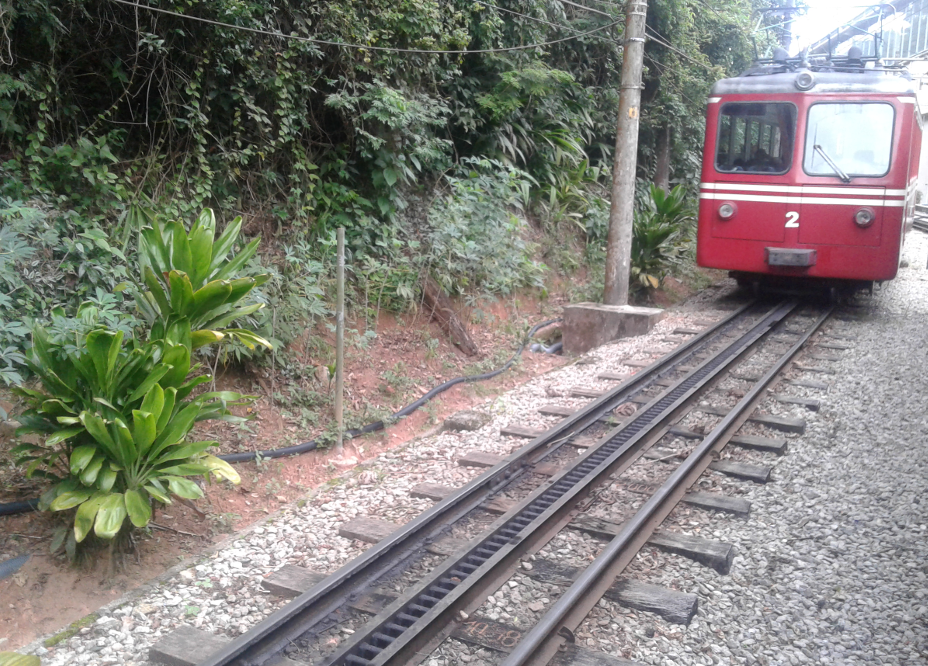
\includegraphics[width=0.48\textwidth]{viacorc}
	\label{fig:viacorc}	
}
%\hspace{0.01\textwidth}
~
\subfloat[Ejemplo de estructura mecánica: atracción mecánica en Montevideo, Uruguay.]{
	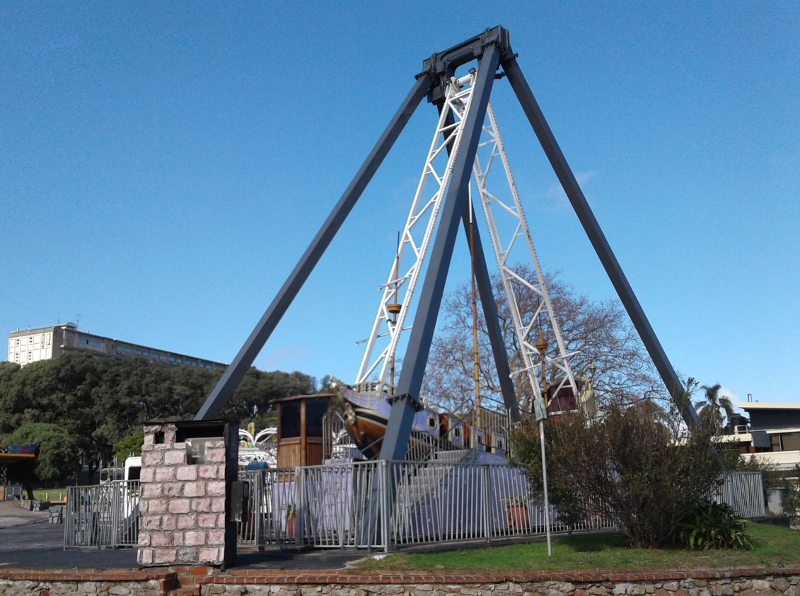
\includegraphics[width=0.47\textwidth]{barcopirata}
	\label{fig:barco}	
}
\caption{Ejemplos de estructuras.}
	\label{fig:ejsestr}
\end{figure}
% ---------------------------------

En este texto se presentan métodos de análisis aplicables principalmente a \underline{estructuras civiles}.









\subsubsection{Clasificación de componentes estructurales}

Las estructuras civiles están formadas por \textit{componentes estructurales}, los cuales son descritos de forma sintética a continuación:
%
\begin{itemize}
	\item \textbf{barra}: elemento con una dimensión (eje) considerablemente mayor que las otras. Soporta tensiones de compresión o tracción según su eje.
	%
	\item \textbf{viga } (de eje recto): elemento con geometría de barra en su configuración natural (sin cargas), que puede ser sometido a fuerzas según su eje (normales) o transversales (cortantes) así como también a momentos según su eje (torsores) o transversales (flectores).
	%
	\item \textbf{pilar}: elemento con geometría de barra que se encuentra sometido a flexión y compresión según su eje siendo la compresión preponderante.
	%
	\item \textbf{cable}: también utilizado como \textbf{tensor}, son elementos de barra sometidos principalmente a tracción que no soportan considerable flexión o compresión según su eje.
	%
	\item \textbf{losa y cáscara}: elementos con dos dimensiones (formando su plano o superficie media) mayores que la otra dimensión. %
	%
	Soportan flexión o tensión con vector contenido en el plano medio. %
	%
	Las losas tienen un plano medio plano, mientras que en las cáscaras este se encuentra dado por una superficie con curvatura no nula.
	%
	\item \textbf{membrana}: elementos superficiales muy flexibles de pequeño espesor que no son capaces de soportar compresión o flexión. %
	%
	En la Figura~\ref{fig:termmadero} se observa la cubierta exterior, de la Terminal Madero de la Ciudad de Buenos Aires, formada y soportada por componentes de membrana, barras, vigas y cables.
	%
	\item \textbf{otros}: existen otros elementos estructurales cuya geometría más compleja no asociados directamente a un estado tensional de los anteriores, por ejemplo: zapatas, cabezales, muros de contención (trabajando como losa o bajo estados planos de deformación) y arcos o vigas de eje curvo.
\end{itemize}

\begin{figure}[htb]
	\centering
	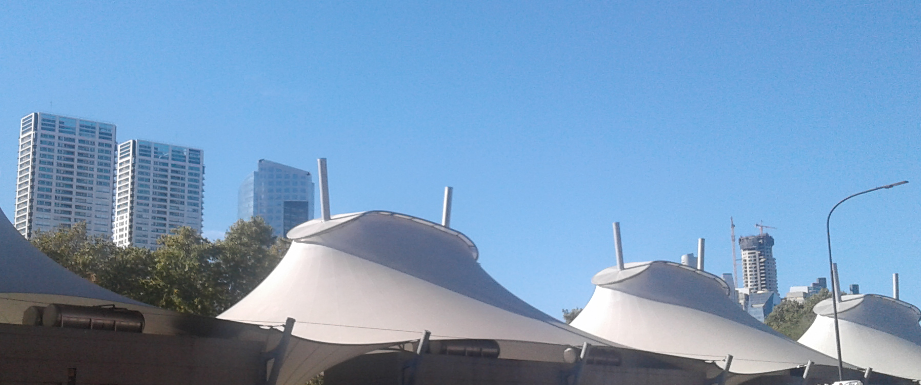
\includegraphics[width=\textwidth]{terminalmadero}
  \caption{Foto exterior de las cubiertas de la Terminal Madero Ciudad de Buenos Aires, Argentina.}
\label{fig:termmadero}
\end{figure}

Un tipo de estructura frecuentemente analizada es el pórtico, o estructura aporticada, la cual está formada por pilares y vigas vinculados por al menos un nudos rígidos o uniones que transmiten momentos. %
%
A continuación se presentan criterios de clasificación de estructuras de acuerdo a los vínculos existentes entre sus componentes.




\subsubsection{Clasificación según sus vínculos}

Se considerarán dos tipos de estructuras de acuerdo a sus vínculos internos:
%
\begin{itemize}
\item \textbf{Estructura reticulada}: formada por barras unidas de forma tal que no se transmiten momentos en todos los nodos de la estructura, es decir que todos los nodos son articulaciones.
%
\item \textbf{Estructura aporticada}: formada por barras unidas donde al menos dos barras están conectadas por un nudo rígido o un vínculo que transmite momentos.
\end{itemize}




\subsubsection{Clasificación según geometría y carga} \label{sec:clasifest}

De acuerdo a su geometría y cargas aplicadas una estructura puede ser clasificada de la siguiente forma.
%
\begin{itemize}
  \item \textbf{Estructura Plana}: Una estructura será considerada \textbf{plana} si se cumplen todas las siguientes condiciones:
    \begin{enumerate}
       \item todos los ejes de sus barras (barras, vigas o pilares) pertenecen a un plano y este plano es plano de simetría de todas las barras de la estructura
       %
       \item todos los vectores de fuerza aplicados a la estructura son vectores contenidos en el plano de simetría de la estructura
       %
       \item todos los momentos aplicados son aplicados en puntos que pertenecen al plano medio de la estructura y están dados por un vector perpendicular al plano de simetría de la estructura
       %
       \item las restricciones cinemáticas son tales que las reacciones correspondientes cumplan con las condiciones anteriores de fuerza y momento.
    \end{enumerate}
  %
  \item \textbf{Estructura Plano-espacial}: Una estructura será considerada \textbf{plano-espacial}, también llamada emparrillado, si se cumple: 
    \begin{enumerate}
	\item todos los ejes de sus barras pertenecen a un plano,
	%
	\item todos los vectores de fuerza aplicados a la estructura son vectores perpendiculares a dicho plano
	%
	\item todos los momentos aplicados son aplicados en puntos que pertenecen al plano de las barras de la estructura y están dados por vectores contenidos en dicho plano
	%
	\item las restricciones cinemáticas son tales que las reacciones correspondientes cumplan con las condiciones anteriores de fuerza y momento.
\end{enumerate}
  
  \item \textbf{Estructura tridimensional}: una estructura será considerada \textbf{tridimensional} si no es clasificada dentro de ninguna de las dos categorías anteriores.
\end{itemize}

\cajaactividad{
	Considere un edificio de viviendas de tres pisos de altura con planta rectangular. %
	%
	Identificar los componentes estructurales de la estructura. %
	%
	Clasifique la estructura de acuerdo a los criterios vistos.}






\subsection{Análisis de estructuras}

Luego de haber definido el término \textit{estructura} se pasa a introducir el concepto de \textit{análisis estructural}. %
%
El análisis es una etapa crucial en el proceso de diseño y verificación de cualquier estructura.

\cajaconcepto{Definición: Análisis estructural}
{El \textit{análisis} de una estructura consiste en la determinación de los \textbf{efectos} (solicitaciones y movimientos) que un sistema de \textbf{cargas} dado produce sobre la \textbf{estructura} y cada uno de los elementos estructurales que la componen.}

El proceso de analizar una estructura puede ser también llamado \textit{resolver} una estructura. %

Las fuerzas aplicadas a los elementos estructuras y la vinculación existente entre estos elementos determinan las deformaciones y solicitaciones de la estructura. %
%
Para definir el tipo de análisis a realizar se deberá categorizar las cargas y vínculos entre componentes. %

A continuación se definen distintos tipos de \textbf{cargas} que suelen ser aplicados a estructuras. Luego se enumeran algunos de los vínculos entre componentes estructurales más importantes.

\subsubsection{Cargas}

Las cargas o fuerzas externas que pueden ser aplicadas a estructuras pueden tener diversas causas, por lo que tendrán diferentes características respecto a: frecuencia de ocurrencia, magnitudes, confiabilidad, etc. Las normas o códigos establecen metodologías para considerar la distinta naturaleza de las acciones al diseñar estructuras.

En este material se considera que toda carga es de tipo \textit{estática} o \textit{permanente}, independientemente de su origen. %
%
Estas cargas son provocadas por acciones cuya magnitud o sentido no varía en el tiempo, como por ejemplo el peso propio de cada elemento estructural. %

Las cargas o esfuerzos producidos por otras acciones como viento, sismos, impactos, etc., deben ser analizadas de forma diferente aplicando modelos numéricos o criterios de diseño específicos definidos por normativas correspondientes.
%
En este texto se asume que, sea cual fuere su origen, toda carga podrá ser considerada como estática. %
%
Existe una importante rama del en la Ingeniería Estructural, enfocada al análisis dinámico de estructuras, en la cual se destacan referencias bibliográficas como \citep{clough1993dynamics}.
%
% ------------------------


\subsubsection{Condiciones de vínculo y apoyo en estructuras}

Los \textit{vínculos a tierra}, o condiciones de apoyo, de cada nodo de una estructura pueden ser clasificados de la siguiente forma:
%
\begin{itemize}
\item \textbf{libre}: un nodo o un extremo de una viga que no está vinculado a tierra o que no tiene desplazamiento ni giro impuesto ni restringido en ninguna dirección o ángulo,
%
\item \textbf{desplazamiento impedido}: vínculo que impide el desplazamiento de un nodo en una o más direcciones,
%
\item \textbf{giro impedido}: vínculo que impide el giro de un nodo según un cierto vector,
%
\item \textbf{resorte de desplazamiento}: vínculo en el cual la fuerza externa aplicada es proporcional y de sentido contrario al desplazamiento desarrollado por el nodo en una cierta dirección,
%
\item \textbf{resorte de giro}: vínculo en el cual el momento externo aplicado es proporcional y de sentido contrario al giro desarrollado por el nodo en una cierta dirección,
%
\item \textbf{vínculo mixto}: vínculo con combinaciones que no pertenecen a ninguna de las categorías anteriores.
%
\end{itemize}

En la Figura~\ref{fig:membr} se muestra parte de la estructura de soporte de la cubierta de la terminal de Madero en Bs. As.. %
%
En la Figura~\ref{fig:artic} se puede ser una materialización de un vínculo que podría considerarse como un apoyo fijo que restringe el desplazamiento de un punto. %
%
El modelado estructural de este vínculo puede ser un problema interesante, donde es necesario estudiar el nivel de restricción real del giro en algunas direcciones. %
%
\begin{figure}[htb]
	\centering
	\subfloat[Elementos de transmisión de cargas y soporte.]{
	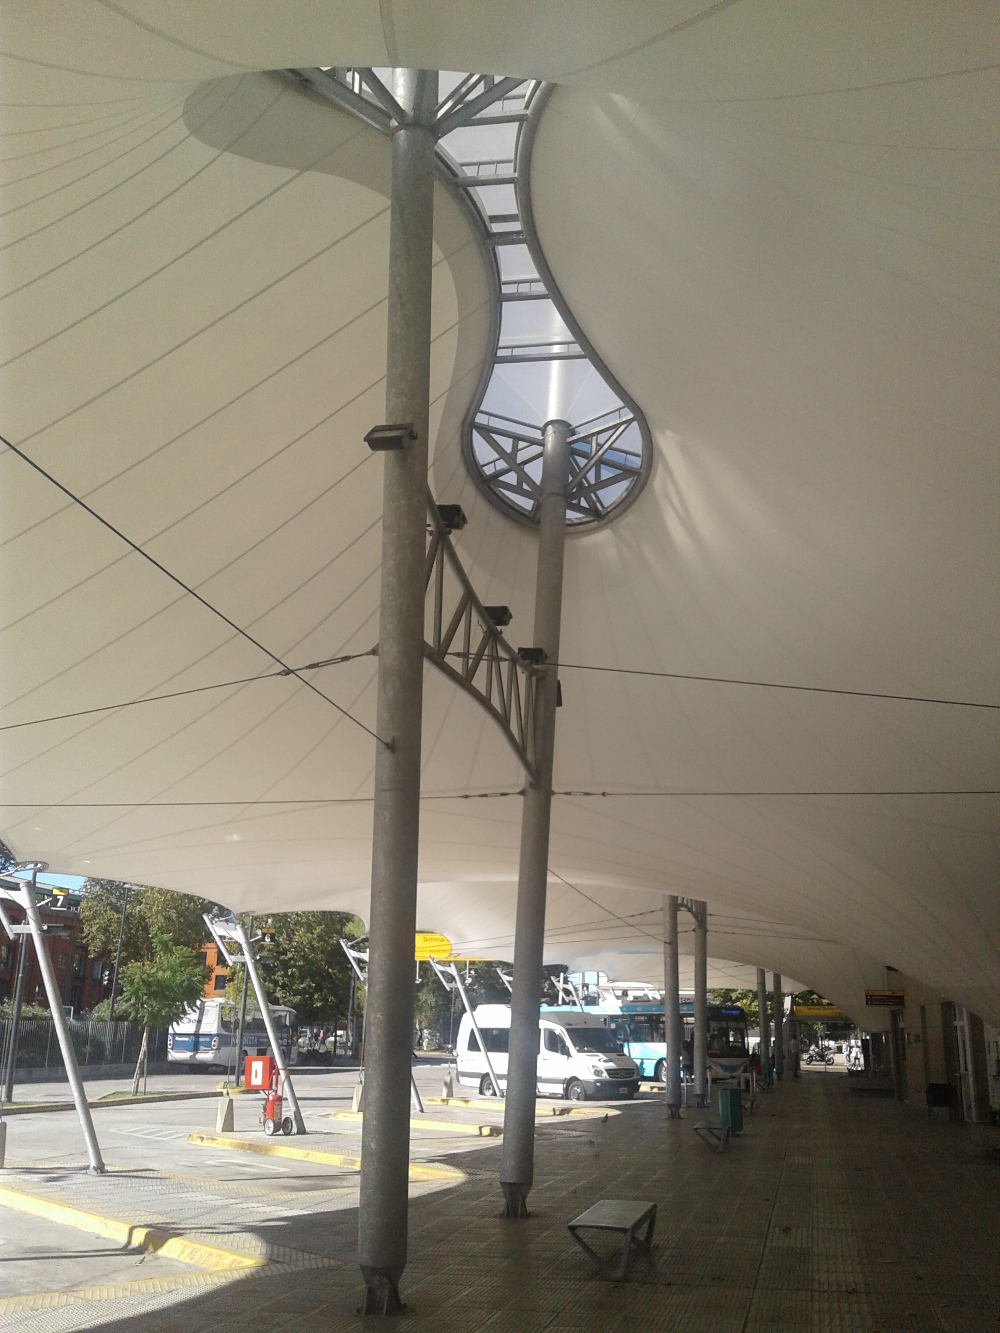
\includegraphics[width=0.38\textwidth]{membranal}
	\label{fig:membr}
}
	\subfloat[Elementos de transmisión de cargas y soporte.]{
	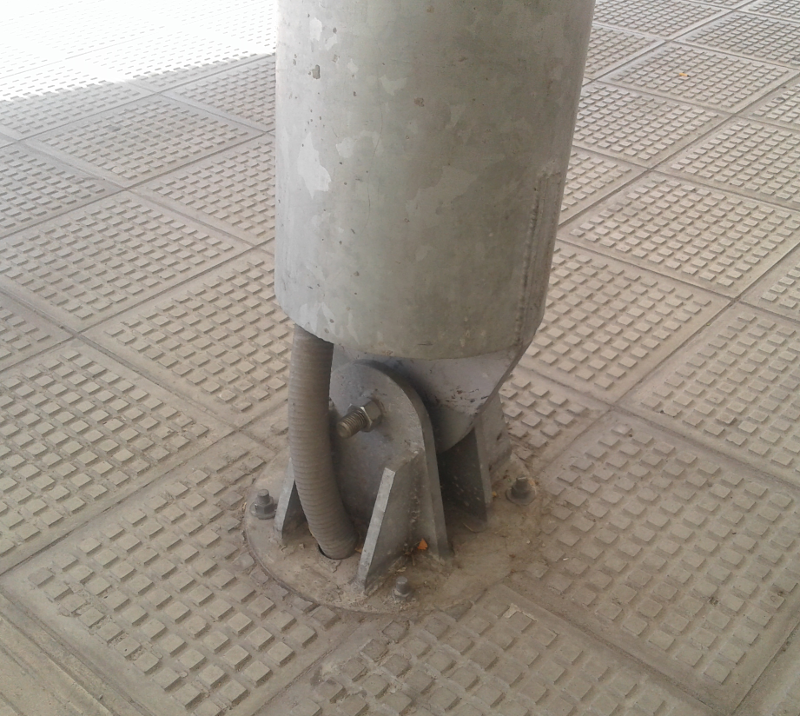
\includegraphics[width=0.57\textwidth]{artic}
	\label{fig:artic}
	}
	\caption{Fotos de interior de terminal Madero, Ciudad de Buenos Aires.  (izq.), vínculo a tierra articulado (der.).}
	\label{fig:bsas}
\end{figure}

\subsubsection{Clasificación de vínculos entre elementos estructurales}

El comportamiento de los elementos estructurales están limitado por los vínculos, que pueden ser clasificados como:
%
\begin{itemize}
\item \textbf{articulación}: nodo que transmite fuerzas y compatibiliza desplazamientos entre barras que llegan a el,
\item \textbf{unión rígida}: nodo que transmite fuerzas y momentos y compatibiliza desplazamientos y giros entre barras que llegan a el,
\end{itemize}

Existen otros tipos de vínculos que pueden ser considerados entre elementos estructurales, pero no serán vistos en el curso.

\cajaactividad{
Enumere las cargas presentes durante la vida útil del edificio de tres pisos considerado en la actividad anterior. %
%
Analice qué tipo de apoyo puede tener la estructura sobre el suelo así como también qué vínculos pueden existir entre los elementos de la estructura.}












\subsection{Modelado estructural}

% presentacion conceptos
El análisis estructural es la herramienta utilizada por profesionales responsables del diseño de estructuras. %
%
El diseño de una estructura consiste en un proceso iterativo en el cual se definen dimensiones de los componentes estructurales, se determinan sus solicitaciones y se verifica que se cumpla con el criterio del profesional y las normativas correspondientes. %
%

Para presentar de forma esquemática el proceso asociado al diseño de una estructura se definen los siguientes conceptos:
%
\begin{itemize}
  \item Estructura Real (ER)
  \item Esquema Básico de Cálculo (EB)
  \item Modelo Numérico (MN)
\end{itemize}
% ---

\paragraph{Estructura Real}
%
El concepto de \textit{Estructura Real} (ER), podrá ser utilizado para referirse a una estructura existente (ya construida), o a aquella que se desea construir y que es imaginada por los diseñadores. %
%
En toda ER se cuenta con una geometría con imperfecciones debidas al procedimiento constructivo. %
Asimismo, la ER está sometida a estados de cargas asociadas al uso efectivo que tiene a lo largo de su vida útil. %
%
Las condiciones de apoyo también son debidas a la interacción de la misma con otros elementos como, por ejemplo, el apoyo sobre un suelo no homogéneo, el cual tiene un comportamiento complejo de alta dificultad para predecir.


\paragraph{Esquema Básico de Cálculo}
%
El \textit{Esquema Básico de cálculo} (EB), es considerado como el modelo simplificado de la estructura que se obtiene al considerar ciertas hipótesis sobre la estructura real. %
%
Como ejemplos se tiene: una geometría idealizada, condiciones de apoyos ideales (por ej. apoyos fijos) o estados de carga hipotéticos, establecidos por normas técnicas y con cierta probabilidad de ocurrencia. %
%
También se pueden incluir aquí las hipótesis sobre el comportamiento constitutivo de los materiales que componen la estructura, frecuentemente estipulado por normas técnicas.

\paragraph{Modelo Numérico}
%
El \textit{Modelo Numérico} (MN) de una estructura es la herramienta que se utiliza para obtener magnitudes solución de las ecuaciones asociadas al EB (es decir, desplazamientos, solicitaciones, tensiones, etc). %
%
Para estas soluciones se debe utilizar algún método numérico para resolver un conjunto de ecuaciones lineales o en algunos casos no lineales \citep{Bazzano2017}. %
%


El proceso de diseño estructural consiste en un procedimiento iterativo que puede ser sintetizado de forma simplificada a través de la siguiente lista de etapas:
%
\begin{enumerate}
  \item establecer \textbf{condiciones} que la ER debe cumplir (arquitectónicas, normativas, etc.)
  %
  \item \textbf{definir un EB} a partir de una primer estimación de secciones, materiales, vínculos entre componentes
  %
  \item a través del uso de un MN \textbf{obtener las solicitaciones} a las que cada componente de la estructura estará sometido
  %
  \item \textbf{diseñar los componentes} de las estructuras para soportar las solicitaciones (acero, secciones, tipo de hormigón, etc.) 
  %
  \item \textbf{verificar} si se cumplen las condiciones definidas en (1): si se cumplen entonces se finalizó, si no se cumplen se debe proponer un nuevo EB recomenzando desde el paso (2).
\end{enumerate}


En este curso se abordará el estudio de métodos analíticos y numéricos para la determinación de solicitaciones y desplazamientos (análisis) de estructuras. %
Esto corresponde a la etapa 3 del proceso de diseño descrito. %
%
En menor medida se realizará diseño de secciones considerando criterios simples de resistencia de materiales sin tomar en cuenta las consideraciones más complejas definidas por las normas técnicas necesarias para el ejercicio profesional. %
%
%A partir de un análisis adecuado del EBCE, el ingeniero decide aspectos como el tipo y cantidad de elementos a utilizar, forma de introducción de los estados de carga y método numérico utilizado para realizar el análisis del problema en función del modelo constitutivo del material.
%

\subsection{Ejemplo: Análisis simplificado de puente metálico}

Para fijar ideas se considera un ejemplo de modelado simple de una estructura compleja. %
%
Con esto, se pretende mostrar parte del proceso de modelado y análisis de una estructura para ilustrar los conceptos introducidos.

En la Figura~\ref{fig:raila} se muestra una foto de un puente metálico, que será considerado como la \textbf{estructura real}. %

\begin{figure}[htb]
  \centering
	\subfloat[Foto de Estructura Real.]{
	  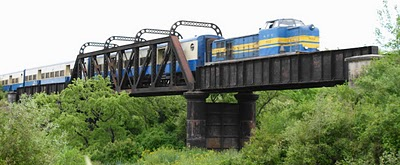
\includegraphics[width=0.7\textwidth]{ferroviario}\label{fig:raila}
    }\\
	\subfloat[Esquema Básico de Cálculo.]{
	  \resizebox{.9\linewidth}{!}{\input{./figs/UT1/reticRail.pdf_tex}}\label{fig:railb}
    }\\
	%
	\subfloat[Diagrama de deformada con factor de escala 10 y escala de colores de tensiones axiales.]%
	{
	  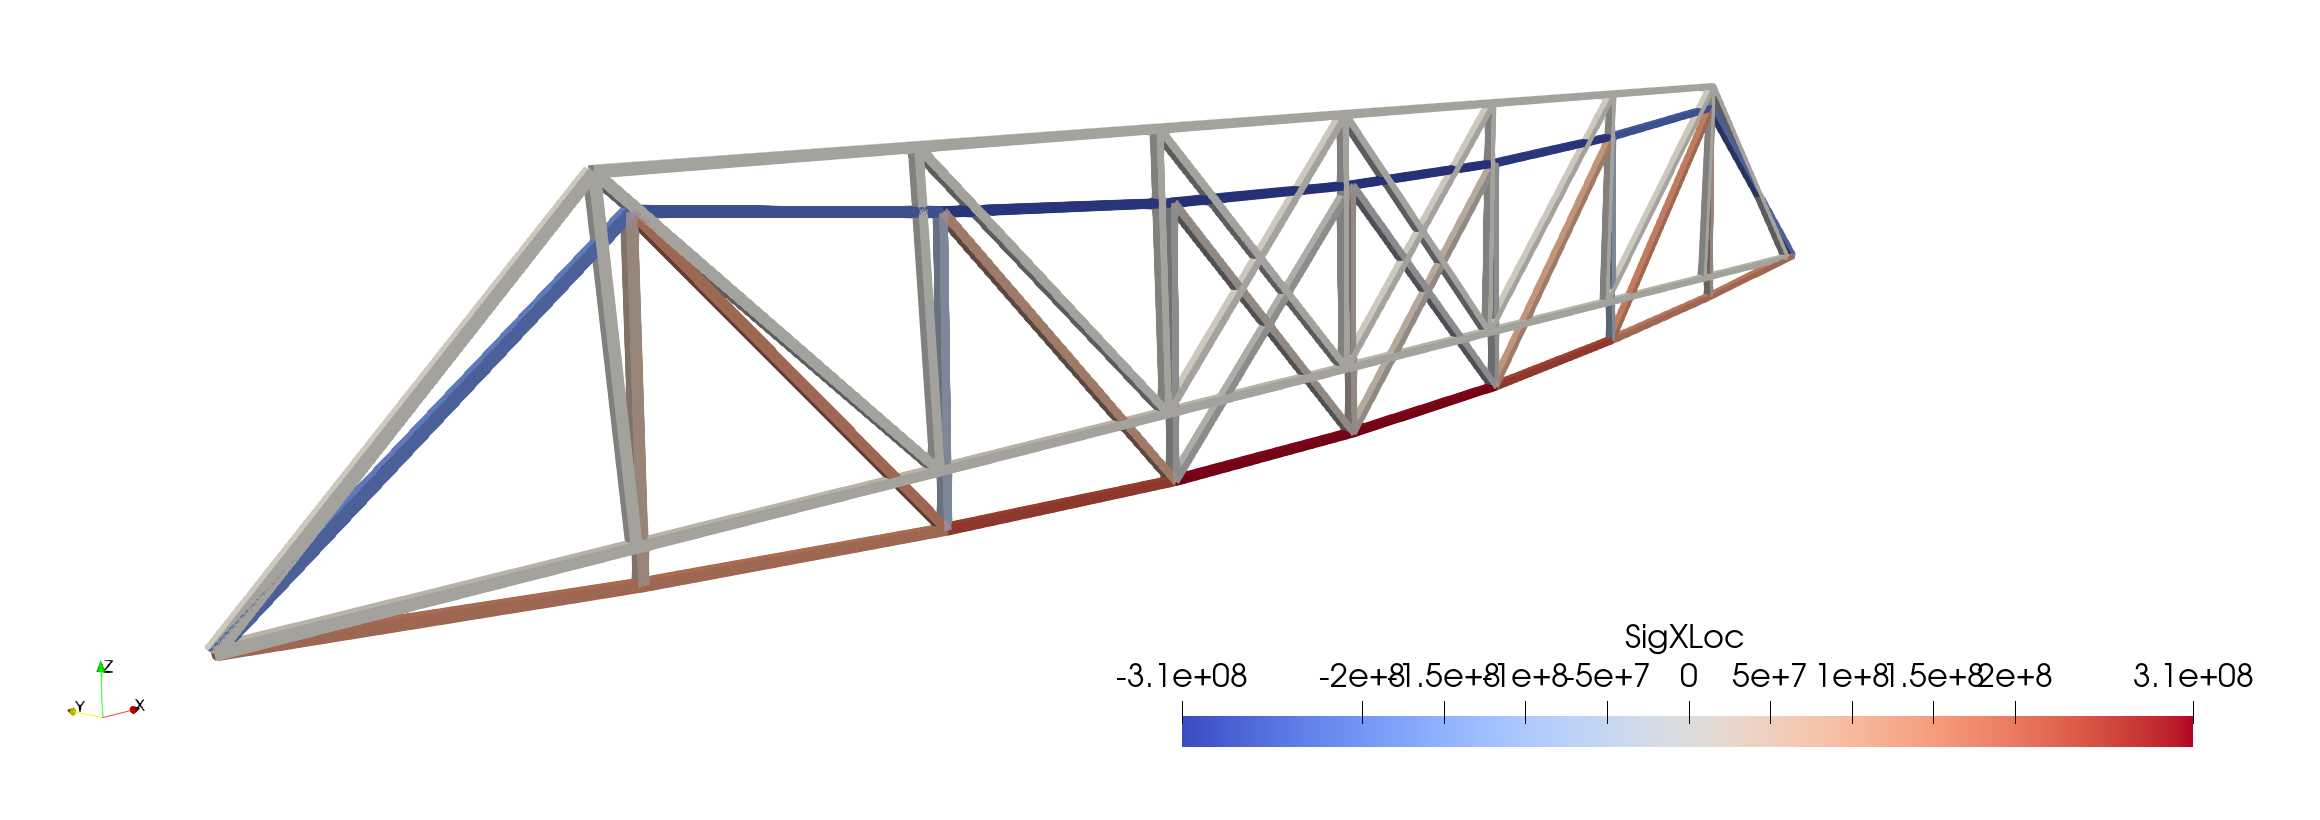
\includegraphics[width=0.9\textwidth]{reticRailDeform}\label{fig:railc}}
\end{figure} 


Para pasar al EB se consideran diversas hipótesis, entre las que se destacan:
\begin{itemize}
  \item las uniones de los perfiles son consideradas como articulaciones,
  %
  \item las cargas puntuales aplicadas en los nodos se consideran de igual magnitud,
  %
  \item se consideran dos reticulados planos con todos sus nodos desplazandose en el plano que los contiene, en lugar de una estructura tridimensional (teniendo en cuenta el estado de cargas simétrico), 
  %
  \item se asume que el material es elástico lineal y que la estructura sufre pequeñas deformaciones y desplazamientos para las cargas aplicadas.
\end{itemize}
%
%
En la Figura~\ref{fig:railb} se muestra el EB obtenido para uno de los reticulados planos considerando las hipótesis mencionadas. %
%
Es importante destacar que otras hipótesis pueden ser consideradas, por ejemplo, el vínculo entre los perfiles puede no ser articulado. %


Finalmente se utiliza el MEF para obtener las magnitudes deseadas resolviendo numéricamente las ecuaciones planteadas por el MN. %
%
Se modela cada barra con un elemento de barra plano de dos nodos, con funciones de interpolación lineales. %
%
Luego de resolver el sistema de ecuaciones lineales correspondiente, se obtienen los desplazamientos y luego de utilizar un factor de escala adecuado (10 en este caso) se obtiene una estructura deformada dada por la Figura~\ref{fig:railc}. La escala de colores representa los valores de tensiones axiales. %
%

En este caso para resolver el Modelo Numérico se utilizó la herramienta de elementos finitos ONSAS \footnote{Código abierto disponible en: \href{https://github.com/onsas}{https://github.com/onsas}}. %
%
El archivo de entrada usado para resolver el reticulado es presentado en el Código~\ref{cod:reticejUT1}.


En este texto nos concentraremos en el estudio de métodos para la resolución del Esquema Básico de Cálculo, a través de la resolución del Modelo Numérico o del uso de soluciones analíticas. %
%
De aquí en adelante se podrá utilizar la palabra estructura para hacer referencia al Esquema Básico de Cálculo.











\section{Ecuaciones de la teoría de vigas} \label{sec:teovigastimo}

En esta sección se repasan conceptos básicos de la teoría de vigas, ya presentada en cursos previos de la materia Resistencia de Materiales. %

Se considera que la viga consiste en un sólido ocupando una región del espacio cuya dimensión longitudinal es considerablemente superior a las dimensiones transversales, y que está sometida a esfuerzos longitudinales y/o transversales. %
%
En la \autoref{fig:viga3d} se muestra un esquema de la geometría considerada. %
%
\begin{figure}[htb]
	\centering
	\def\svgwidth{0.5\textwidth}
	\input{figs/UT1/viga3d_amano.pdf_tex}
	\caption{Esquema tridimensional de viga y sistema de coordenadas considerado.}
	\label{fig:viga3d}
\end{figure}

%
En este material y en el curso se tendrán en cuenta las siguientes hipótesis/convenciones:
%
\begin{itemize}
	\item la sección transversal es uniforme a lo largo de la dirección $x$, %
	\item el eje $\bfe_x$ pasa por los baricentros de las secciones transversales, denotados por $G$,
	\item los ejes $\bfe_y$ y $\bfe_z$ son ejes principales de la sección transversal,
	\item y el plano $x-y$ es plano de simetría de la sección transversal y de la viga.
\end{itemize}


\subsection{Ecuaciones de la teoría de vigas en flexión pura}

Se pasa ahora a considerar el plano $x-y$ y que la viga está sometida a un estado de flexión pura. %
%
En esta sección se presentan esquemáticamente las ecuaciones más importantes de la teoría de vigas, la cual se puede ver de forma más extendida en \citep{Timoshenko1940a}. %

En la \autoref{fig:viga2d} se muestra el esquema plano de la viga deformada. %
%
La función $v(x)$ representa el desplazamiento según $\bfe_y$ del baricentro de aquella sección transversal ubicada en la posición $x$ y $\theta(x)$ el ángulo que gira dicha sección, o también el ángulo que forma la tangente a la curva deformada con el eje $x$. %

\begin{figure}[htb]
	\centering
	\def\svgwidth{0.65\textwidth}
	\input{figs/UT1/viga2d.pdf_tex}
	\caption{Esquema plano de viga deformada.}
	\label{fig:viga2d}
\end{figure}
%
%

A partir de la hipótesis de que las secciones planas permanecen planas y perpendiculares a la curva de los baricentros en la deformada, se obtiene la expresión de la deformación axial en cualquier punto:
%
\begin{equation}
\varepsilon(x,y) = \frac{ (\rho(x) -y) d\theta - \rho(x) d \theta }{ \rho(x) d \theta} = \frac{-y}{\rho(x)},
\end{equation}
donde se omitió el subíndice $x$ de la deformación axial y $\rho(x)$ es el radio de curvatura de la deformada y está dado por
%
\begin{equation}
\rho(x) = \frac{ds}{d\theta}(x).
\end{equation}
%
donde $s(x)$ es la longitud de la curva deformada en la posición $x$.
%
La curvatura de la curva deformada está dada por
\begin{equation}
\kappa (x) = \frac{1}{\rho(x)} = \frac{1}{\dfrac{ds}{d \theta} (x)}.
\end{equation}

Se procede a buscar una forma de calcular la función $\frac{ds}{d\theta}$. %
Utilizando la regla de la cadena se obtiene:
%
\begin{equation}\label{eqn:dsdtheta}
\dfrac{ds}{d \theta} = \frac{ds}{dx} \frac{dx}{d\theta}
\end{equation}


Para el primer factor del segundo miembro se tiene que la función de la longitud de curva deformada puede ser calculada fácilmente en función de $x$ usando la definición de la longitud de curva considerando la parametrización $(x(t)=t,y(t)=v(t))$, obteniendo:
%
\begin{equation}
s(x) = \int_0^x \sqrt{1+  \left( \frac{d v}{d t}(t)\right)^2} dt
\end{equation}
%
por lo tanto se cumple:
\begin{equation}\label{eqn:dsdx}
\frac{ds}{dx} (x) = \sqrt{1+ \left( \frac{ d v}{d x}(x)  \right) ^2}.
\end{equation}

Por otra parte, para obtener una expresión del segundo factor del miembro derecho de la Ecuación~\eqref{eqn:dsdtheta}, se sabe que se cumple:
%
\begin{equation}
\tan(\theta(x) ) = \frac{d v}{d x} (x)
\end{equation}
%
por lo que se puede obtener la función $\theta(x)$ como:
%
\begin{equation}
\theta(x) = \arctan \left( \frac{d v}{d x} (x) \right).
\end{equation}

Usando la identidad:
%
\begin{equation}
\frac{d \arctan (u)}{d u} = \frac{1}{1+ u^2},
\end{equation}
%
y la regla de la cadena se obtiene:
\begin{equation}
\frac{d \theta }{d x} (x) = \frac{1}{ 1 + \left( \frac{dv}{dx} (x)\right)^2} \frac{d^2 v}{d x^2}(x) .
\end{equation}

Usando el teorema de la función inversa se tiene que 
$$
\frac{d x}{d\theta}\left( \theta(x) \right) = \frac{1}{\dfrac{d \theta}{dx}(x)},
$$
por lo tanto se obtiene
%
\begin{equation}\label{eqn:dxdtheta}
\frac{d x}{d\theta}(\theta(x)) =  \left( 1 + \left( \frac{dv}{dx} (x)\right)^2 \right)  \frac{1}{  \frac{d^2 v}{d x^2}(x)}
\end{equation}
%
sustituyendo las ecuaciones \eqref{eqn:dsdx} y \eqref{eqn:dxdtheta} en la Ecuación~\ref{eqn:dsdtheta} y aplicando la definición de la curvatura se obtiene la expresión:
%
\begin{equation}
\kappa(x) = \frac{d^2 v}{d x^2} \frac{1}{\left( 1+ \left( \frac{dv}{d x}\right)^2 \right)^{3/2}}.
\end{equation}
%

En el caso de que la viga desarrolle pequeños giros $\theta \ll 1 $, o que esa sea la hipótesis considerada, se consideran los siguientes desarrollos de Taylor respecto a cero:
%
\begin{equation}
\tan(\theta) \approx \theta  \quad \text{y}\quad \left( 1+ \left( \frac{dv}{d x}\right)^2 \right) = (1 + \tan(\theta)^2 ) \approx 1,
\end{equation}
%
por lo que se obtiene una nueva expresión simplificada de la curvatura:
%
\begin{equation}\label{eqn:defcurv}
\kappa (x) =  \frac{d\theta}{d x}(x) = \frac{d^2 v}{d x^2}.
\end{equation}

La deformación axial en la sección $x$ y en la \textit{fibra} ubicada en la posición $y$ puede ser también aproximada como:
\begin{equation}\label{eqn:epstimo}
\boxed{
	\varepsilon(x,y) = -y \frac{d^2 v}{d x^2} (x) = -y \frac{d \theta}{d x} (x),
}
\end{equation}
%
aproximación que será útil para el desarrollo del elemento finito de viga.




\section{Conceptos básicos de Elasticidad Lineal}

La teoría de la mecánica del continuo permite formular y aplicar modelos numérico-matemáticos para estimar la deformación de cuerpos sólidos, al ser sometidos a esfuerzos conocidos considerando condiciones de apoyo adecuadas. %
%
En esta sección se presentan esquemáticamente algunos conceptos de la teoría de Elasticidad Lineal importantes para el posterior desarrollo de los conceptos del texto.


\subsection{Problema de Elasticidad Lineal}

En esta sección se presentan los conjuntos de ecuaciones fundamentales necesarios para formular el Problema de Elasticidad Lineal (PEL) con el objetivo de analizar cualquier estructura o sólido. Estas ecuaciones son:
\begin{itemize}
\item \textbf{Ecuaciones de equilibrio}: relaciones entre  tensiones de elementos estructurales y fuerzas externas
\item \textbf{Ecuación constitutiva}: relación entre tensiones y deformaciones de elementos
\item \textbf{Relaciones cinemáticas}: relación entre deformaciones y desplazamientos
\item \textbf{Condiciones de contorno}: valores conocidos de desplazamientos y fuerzas externas
\end{itemize}

\subsubsection*{Ecuaciones de equilibrio}

Sea un sólido ocupando una región $\Omega$ del espacio, como el mostrado en la Figura~\ref{fig:diagrama_solido}, sometido a una fuerza de volumen $\bfb$, cuya inercia puede ser despreciada, las ecuaciones puntuales de equilibrio están dadas por:
%
\begin{equation}\label{eqn:equil}
\left\{
\begin{array}{lr}
  \nabla \cdot \bfsig(\bfx) + \bfb = \bszer \qquad &\forall \bfx \, \text{en } \Omega\\
  \bfsig(\bfx) = \bfsig(\bfx)^T \qquad  &\forall \bfx\, \text{en } \Omega
\end{array}
\right.
\end{equation}
%
donde $\bfsig(\bfx)$ es el tensor de tensiones en el punto $\bfx$. %
%

\begin{figure}[htb]
\centering
  \def\svgwidth{0.4\textwidth}
  \input{figs/UT1/diagrama_solido.pdf_tex}
\caption{Esquema de cuerpo sólido sometido a fuerzas externas.}
\label{fig:diagrama_solido}
\end{figure}

%
Se asumirá de aquí en adelante que el tensor de tensiones es simétrico en todo punto $\bfx$ de $\Omega$ aunque no sea aclarado. %
%
Por simplicidad de notación se omitirá el punto $\bfx$ de aquí en adelante. %

\subsubsection*{Ecuación constitutiva}

Para materiales hiperelásticos, las tensiones están relacionadas de forma directa con el tensor de deformaciones $\bfvarep$ a través de la ecuación
%
\begin{equation}\label{eqn:hyper}
  \bfsig = \frac{\partial \Psi }{\partial \bfvarep} (\bfvarep),
\end{equation}
%
donde $\Psi$ es la función de densidad de energía de deformación y $\bfvarep$ es el tensor de deformaciones infinitesimales.

Para materiales con comportamiento elástico lineal se tiene
%
\begin{equation}
\Psi (\bfvarep) = \frac{1}{2} \bfvarep : \bbC[  \bfvarep],
\end{equation}
donde $\bbC$ es el tensor constitutivo. %
%
Usando la Ecuación~\eqref{eqn:hyper} se obtiene la ecuación constitutiva en la forma: %
%
\begin{equation}
  \sigma = \bbC [\bfvarep],
\end{equation}
%
es decir una relación lineal entre tensión y deformación.

En este texto se consideran materiales isótropos, los cuales tienen igual comportamiento constitutivo en todas las direcciones. %
%
Se puede mostrar que el tensor constitutivo está dado por dos parámetros (parámetros de Lamé), permitiendo obtener la siguiente expresión de la ecuación constitutiva:
%
\begin{equation}\label{eqn:eccons}
\bfsig (\bfvarep) = \lambda \tra (\bfvarep) \bfI + 2 \mu \bfvarep,
\end{equation}
%
donde Tr es la función traza y $\lambda$ y $\mu$ son los parámetros de Lamé. %
%
Estos últimos están relacionados con el módulo de Young $E$ y el coeficiente de Poisson $\nu$ a través de las expresiones
%
\begin{equation}
 \lambda = \frac{E \nu}{(1+\nu)(1-2 \nu)} \quad \text{y} \quad
 \mu = \frac{E}{2(1+\nu)}.
\end{equation}

El parámetro $\mu$ es llamado módulo de corte y puede también ser denotado como $G$.

Existen diversos materiales, como por ejemplo la madera, para los cuales no se cumple la propiedad de isotropía y el tensor $\bbC$ tiene una expresión dependiente de una mayor cantidad de parámetros. %
%
La madera es uno de los materiales con comportamiento anisótropo más utilizados en construcción \citep{Pereira2014a}, siendo sus propiedades según la dirección de las fibras, aquellas de mayor relevancia e interés de estudio \citep{PerezZerpa2017}. %
%
Otro material con comportamiento anisótropo presente en la naturaleza es el tejido arterial \citep{Holzapfel2000}. %
%
En este texto se hará foco en materiales isotrópicos. %
% ------------------


\subsubsection*{Relaciones cinemáticas}

El tensor de deformaciones está relacionado con el campo de desplazamientos $\bfu$ a través de la expresión:
%
\begin{equation}\label{eqn:relcin}
\varepsilon = \frac{1}{2} ( \nabla \textbf{u} + \nabla \textbf{u}^T ).
\end{equation}

\subsubsection*{Condiciones de contorno}

Finalmente se presentan las condiciones de contorno en desplazamientos sobre $\Gamma_\bfu$ y en tensiones sobre $\Gamma_\bft$
%
\begin{equation}\label{eqn:condcont}
\left\{
\begin{array}{lr}
\bfu = \hat{\bfu} &  \text{en } \Gamma_\bfu \\
\bfsig  [\bfn] = \hat{\bft} & \text{en } \Gamma_\bft
\end{array}
\right.
\end{equation}
%
donde $ \hat{\bfu}$ es el campo vectorial de desplazamientos impuestos o conocidos, y $\hat{\bft}$ es el campo vectorial de vectores tensión aplicados.


\subsubsection*{Problema de Elasticidad Lineal}

El PEL consiste en encontrar las magnitudes: $\bfsig$, $\bfvarep$ y $\bfu$ que verifican simultáneamente las condiciones establecidas por las ecuaciones: \eqref{eqn:condcont},\eqref{eqn:eccons}, \eqref{eqn:equil} y \eqref{eqn:relcin}. %
Esta es usualmente llamada la formuación fuerte del problema de Elasticidad Lineal.



\subsection{Principios energéticos en elasticidad lineal}

A partir de las ecuaciones de la formulación fuerte del PEL es posible obtener formulaciones débiles o integrales, las cuales facilitan la posterior presentación de métodos numéricos de resolución.


\subsubsection{Teorema de trabajo virtual}

Si se considera un campo tensorial $\bfsig $ en equilibrio con las fuerzas externas y un campo de desplazamientos virtuales $\bfw$ compatible con las condiciones cinemáticas de contorno, entonces se cumple que:
%
\begin{equation}
\int_{\Omega} \bfsig : \bfvarep (\bfw) dV = \int_{\Gamma_t}  \hat{\bft} \cdot \bfw d S,
\end{equation}
%
donde el miembro izquierdo representa el trabajo de las fuerzas internas y el miembro derecho el trabajo de las fuerzas externas.

Esta relación permite plantear el problema de encontrar $\bfsig$ como el problema de encontrar cuál es el campo tensorial que verifica la igualdad anterior para cualquier campo de desplazamientos virtual.

\begin{equation}
\int_{\Omega} \bfsig : \bfvarep (\bfw) dV = \int_{\Gamma_t}  \hat{\bft} \cdot \bfw d S \qquad \forall \bfw \in \mcV_{u}
\end{equation}
%
donde $\mcV_u$ es el conjunto de desplazamientos virtuales compatibles con los vínculos de apoyo.

Esta relación puede ser obtenida a partir de las ecuaciones de equilibrio puntual y las condiciones de contorno mecánicas.

\subsubsection{Formulación debil del problema de elasticidad lineal}

Considerando la ecuación constitutiva del material elástico lineal se puede reescribir la ecuación anterior obteniendo una nueva formulación del PEL. Esta formulación consiste en hallar el campo de desplazamientos $\bfu$ tal que se cumple:
%
\begin{equation}
\int_{\Omega} \bbC[ \bfvarep (\bfu)] : \bfvarep (\bfw) dV = \int_{\Gamma_t}  \hat{\bft} \cdot \bfw d S \qquad \forall \bfw \in \mcV_{u}.
\end{equation}

Este es el tipo de expresiones que posibilitan el desarrollo, de forma directa, de métodos numéricos para la resolución eficiente del problema, en particular el Método de los Elementos Finitos \citep{Hughes1987a}.

\subsubsection{Principio de mínima energía potencial total}

Es también posible obtener las expresiones anteriores a partir de un enfoque basado en principios energéticos.

Se define la energía potencial de las fuerzas externas como:
%
\begin{equation}
\Pi_{ext}(\bfu) = -\int_{\Omega} \bfb \cdot \bfu \dif V - \int_{\Gamma_\bft} \hat{ \bft} \cdot \bfu \dif S.
\end{equation}
%
Por otra parte, la energía potencial de deformación está dada por la integral de la densidad de energía de deformación:
%
\begin{equation} \label{eqn:energbarra}
  \Pi_{int}(\bfu) = \int_{\Omega}
  \Psi (\bfu) \dif V = \frac{1}{2} \int_{\Omega} \bbC[ \bfvarep (\bfu)] : \bfvarep (\bfu) dV.
\end{equation}

Se define la energía potencial total del sistema para el campo de desplazamientos $\bfu$, denotada por $\Pi(\bfu)$ y dada por la expresión:
%
\begin{equation}
\Pi(\bfu) = \Pi_{int}(\bfu) + \Pi_{ext}(\bfu)
\end{equation}

\paragraph{Principio de mínima energía potencial}
El principio establece que, dado un problema de elasticidad lineal con condiciones de contorno de tensión en $\Gamma_\bft$, condiciones de contorno en desplazamientos en $\Gamma_\bfu$, un campo de desplazamientos $\bfu$ es solución del problema si verifica 
\begin{equation}
\bfu = \arg\min_{\bfu\in\mcU} \Pi(\bfu)
\end{equation}
%
donde $\mcU$ es el conjunto de los campos de desplazamientos cinemáticamente admisibles, es decir que cumplen $\bfu=\hat{\bfu}$ en $\Gamma_{\bfu}$. %
%
% ------------------------------


Utilizando la definición de mínimo o las condiciones de optimalidad se puede mostrar la equivalencia entre el principio de mínima energía potencial y el teorema de trabajo virtual. %
%
En \citep{CanelasElasticidad} se presentan desarrollos de este tipo para el caso de sólidos, mientras que en este curso aplicará el principio  en el contexto de cada teoría estructural particular.




\subsubsection{Teorema de reciprocidad de Betti} \label{sec:Betti}

El Teorema de Betti puede ser enunciado de la siguiente forma:
Sea una estructura ocupando la región $\Omega$, %
%
dado un conjunto de fuerzas externas aplicadas: $\bfb_A$ y $\bft_A$, las cuales producen desplazamientos $\bfu_A$ y dado por otra parte un conjunto de fuerzas externas $\bfb_B$ y $\bft_B$ que producen desplazamientos $\bfu_B$, entonces se cumple:
%
\begin{equation}
\int_{\Omega} \bfb_A \cdot \bfu_B \dif V + \int_{\Gamma_\bft} \bft_A \cdot \bfu_B \dif S
=
\int_{\Omega} \bfb_B \cdot \bfu_A \dif V + \int_{\Gamma_\bft} \bft_B \cdot \bfu_A \dif S.
\end{equation}


Este teorema será aplicado en unidades temáticas posteriores al desarrollo de métodos de determinación de líneas de influencia en pórticos.

\subsection{Aplicación al desarrollo de teorías estructurales}

Los principios energéticos permiten obtener, a través del uso de ciertas simplificaciones o aproximaciones respecto al comportamiento de los sólidos, expresiones de las ecuaciones de mayor facilidad de resolución. %
%
En esta sección se presenta el desarrollo de la teoría de barras articuladas.


Las teorías de estructuras pueden ser desarrolladas tanto a partir de hipótesis respecto al movimiento que sufren los puntos del cuerpo sólido como a partir de los estados tensionales que el sólido es capaz de soportar. %
%
En este caso se consideran las hipótesis cinemáticas como punto de partida. %

\subsubsection{Teoría de barras articuladas}

%
En el caso del elemento de barra sometido a esfuerzo según su eje, se considera que las tensiones axiales internas son uniformes en la sección transversal y el campo vectorial de desplazamientos corresponde a una deformación uniaxial. %
%
Se considera que no hay fuerzas de volumen aplicadas en la barra, por lo que solo se tendrán tensiones en los extremos. %
%
Si se considera que el eje $\bfe_x$ coincide con el eje de la barra entonces el tensor de deformaciones está dado por el correspondiente a un ensayo uniaxial es decir:
%
\begin{equation} \label{eqn:epsbarras}
\bfvarep (\bfx) = \left[
\begin{matrix}
\varep_x & 0 & 0\\
0 & -\nu \varep_x & 0\\
0 & 0 & -\nu \varep_x
\end{matrix}\right]  \quad \forall \bfx\in\Omega
\end{equation}
%
lo que corresponde a un movimiento en el que las secciones perpendiculares al eje se mantienen planas y perpendiculares al eje y solamente modifican su área. %
%

Sustituyendo en la ecuación constitutiva se tiene:
%
\begin{equation} \label{eqn:sigmaBarra}
\bfsig = \left[
\begin{matrix}
	E\varep_x & 0 & 0\\
	0 & 0 & 0\\
	0 & 0 & 0
\end{matrix}\right],
\end{equation}
%
por lo que la única ecuación constitutiva relevante en los principios energéticos es $\sigma_x = E \varep_x$.

A partir de la ecuación de equilibrio y considerando que no hay fuerzas de volumen aplicadas en el interior de la barra se tiene que
\begin{equation}
\frac{\partial \sigma_x}{\partial x} = 0 = E \frac{\partial \varep_x}{\partial x},
\end{equation}
por lo tanto la deformación es uniforme en la barra y además puede ser escrita en términos de los desplazamientos de los nodos de los extremos. Si $u_2$ es el desplazamiento del nodo del extremo derecho y $u_1$ el del extremo izquierdo, se tiene:
\begin{equation}
\varep_x = \frac{ u_2-u_1}{\ell}
\end{equation}
donde $\ell$ es el largo de la barra.

Sustituyendo estas expresiones en la definición de energía potencial se obtiene una expresión de $\Pi$ en función de los desplazamientos nodales:
%
\begin{equation}
\Pi(u_1,u_2) = \frac{1}{2} \int_{\Omega} E \frac{1}{\ell^2} (u_2-u_1)^2 dV - F_1 u_1 - F_2  u_2
\end{equation}

calculando la integral y derivando respecto a $u_1$ y $u_2$ se obtiene:

\begin{equation}
\nabla \Pi(u_1,u_2) = 
 \frac{EA}{\ell}
  \left[
\begin{matrix}
1 & -1 \\
-1 & 1 
\end{matrix}\right] 
  \left[
\begin{matrix}
u_1  \\
u_2 
\end{matrix}\right]
- 
  \left[
\begin{matrix}
F_1  \\
F_2 
\end{matrix}\right]
\end{equation}

por lo que la condición de punto crítico es
\begin{equation}\label{eqn:criticoBarra}
 \frac{EA}{\ell}
\left[
\begin{matrix}
1 & -1 \\
-1 & 1 
\end{matrix}\right] 
  \left[
\begin{matrix}
u_1  \\
u_2 
\end{matrix}\right]
= 
\left[
\begin{matrix}
F_1  \\
F_2 
\end{matrix}\right]
\end{equation}

Varios ejemplos de teorías estructurales de interés para el análisis de estructuras civiles se pueden encontrar en \citep{Onate2013}. %
%
Durante el curso se abordarán las teorías de vigas y pórticos así como también se introducirá la teoría de losas.



\section{Grados de indeterminación}

Existen diversos métodos disponibles para el análisis de una estructura, por lo tanto, es útil identificar qué tipo de métodos son los más adecuados antes de iniciar el análisis estructural. %
En esta sección se presentan propiedades geométricas (valores numéricos) que pueden ser calculados antes del análisis para tomar una mejor decisión sobre el método a utilizar.

Los grados de indeterminación estática y cinemática son valores dados por la geometría y los vínculos entre componentes de la estructura. %
%
Estos valores numéricos permiten estimar la complejidad de la resolución usando dos métodos analíticos presentados el curso: el \textit{Método de las Fuerzas} y el \textit{Método de los Desplazamientos}. %
%


\subsection{Grado de indeterminación estática}

% -------------------------
El grado de indeterminación estática (también llamado \textit{grado de hiperestaticidad}) es un valor numérico definido por la diferencia entre: el número de incógnitas de fuerza y el número de ecuaciones de equilibrio. %
%
La metodología de cálculo presentada en esta sección está basada en \citep{CerveraRuiz2002ii}. %
%
En esta metodología se parte de un EBC, opcionalmente se pueden considerar componentes separadas de la estructura y se aplica una ecuación para el cálculo.

Las \textbf{incógnitas de fuerza} son aquellas necesarias para determinar completamente el \textit{\textbf{estado tensional}} de toda la estructura. En las estructuras consideradas en este texto, estas incógnitas son:
%
\begin{itemize}
	\item $n_S$: solicitaciones a determinar y fuerzas debidas a \textit{vínculos internos} de cada componente,
	\item $n_R$: reacciones dadas por \textit{vínculos externos}.
\end{itemize}


Por otra parte para calcular el número de ecuaciones con que se cuenta se define:
%
\begin{itemize}
	\item $n_C$: es el número de componentes o partes en la que se separa la estructura para el cálculo,
	\item $n_E$: el número de ecuaciones de equilibrio para cada parte.
	\end{itemize}

La expresión matemática del grado de indeterminación estática puede ser presentada como:
%
\begin{equation} \label{eqn:gradoh}
gh = n_R + n_S - n_C \, n_{E}.
\end{equation}

Como ejemplo se presentan las estructuras de la Figura~\ref{fig:ejemghSimp}, formadas por un único componente y con diferente cantidad de reacciones externas. Dado que no se cortan o liberan vínculos internos de la estructura no hay $n_S$.

\begin{figure}[htb]
\centering
 \def\svgwidth{0.95\textwidth}
  \input{figs/UT1/ejemplos_basicosGradoHiper.pdf_tex}
  \caption{Ejemplos simples de cálculo de grado de hiperestaticidad.}
  \label{fig:ejemghSimp}
\end{figure}

En la Figura~\ref{fig:ejemghMed}. se muestra un reticulado, donde nuevamente si se desacopla en $n_C=3$ componentes una por barra, se tiene que cada articulación introduce dos vínculos a determinar. Por lo tanto $gh = 2+1+2+2+2-3\times 3 = 0$.

\begin{figure}[htb]
	\centering
	\def\svgwidth{0.6\textwidth}
	\input{figs/UT1/ejemplos_mediosGradoHiper.pdf_tex}
	\caption{Ejemplo de cálculo de grado de hiperestaticidad en reticulado.}
	\label{fig:ejemghMed}
\end{figure}

Este cálculo también puede ser realizado considerando la estructura como una única componente. Más adelante se mostrará una ecuación práctica para el cálculo de $gh$ en reticulados planos.

\paragraph{Analogía con cálculo a partir de grados de libertad} %
El cálculo presentado es análogo al utilizado en otros cursos, en los cuales se considera el número de grados de libertad total de las estructuras (en el ejemplo $3\times 3$) y se van restando los vínculos que restringen el movimiento entre barras y a tierra ($-2-1-2-2-2$) por lo que se obtiene un valor opuesto al $gh$.

\paragraph{Clasificación de estructuras según grado de hiperestaticidad} %
Las estructuras pueden ser clasificadas según su grado de hiperestaticidad:
\begin{itemize}
	\item \textit{estáticamente determinada} (o isostática): es aquella estructura cuyo estado tensional puede ser determinado usando únicamente ecuaciones de equilibrio, por lo tanto:
	$$
	gh = 0
	$$
	
	\item \textit{hiperestáticas}: es aquella estructura para la cual no es posible determinar el estado tensional usando únicamente equilibrio, es decir:
	$$
	gh > 0.
	$$
	En este caso deben ser utilizadas oras ecuaciones como por ejemplo compatibilidad de desplazamientos. %
	
	\item \textit{hipoestáticas} (o mecanismos): este último caso corresponde a estructuras en las cuales se tienen más ecuaciones que incógnitas por lo tanto
	$$
	gh <0.
	$$
\end{itemize}



\subsubsection{Grado de hiperestaticidad externa}
%
Si se considera a la estructura como un conjunto donde solamente se desea determinar las reacciones, es posible definir el grado de hiperestaticidad externa como
%
\begin{equation}
gh_E = n_{R} - 1 \times n_{E}
\end{equation}
%
donde $n_R$ es nuevamente el número de reacciones y $n_E$ es el número de ecuaciones del conjunto de la estructura. %
%
En el ejemplo visto en la Figura~\ref{fig:ejemghSimp} a la derecha, se tiene: $gh_E = 4 - 3 = 1$. %


%\cajaactividad{
%	Demostrar que: todo reticulado con $gh_E = 0$  y sin barras cruzadas, cumple: tiene $gh\leq 0$.}

Finalmente, se puede usar los valores $gh_E$ y $gh$ para formular una condición \textbf{necesaria} que una estructura \textit{isostática} debe cumplir. %
%
Se dice que:
%
$$
\boxed{
\text{Estructura isostática} \quad \Rightarrow \quad gh_E = 0 \, \textbf{y} \, gh = 0.
}%
$$
% -------------------------


Existen casos de particulares, de estructuras en las cuales aún siendo isostáticas el grado de hiperestaticidad externa es mayor que cero, como por ejemplo la mostrada en la Figura~\ref{fig:hipereje}. %
%
Esto se debe a que la estructura está conformada por barras no conectadas entre sí como ocurre en la mostrada en las Figuras \ref{fig:ejemghMed} o \ref{fig:retic_gh}. %
%
Esta peculiaridad teórica no será relevante al momento de aplicación práctica del Método de las Fuerzas como se verá en la UT siguiente.


\subsubsection{Cálculo general de grado de hiperestaticidad en pórticos/vigas/barras planos}

En el caso de estructuras de pórticos planos, la determinación del estado tensional requiere conocer 3 solicitaciones en todo punto: directa, cortante y momento. %
%
A modo de ejemplo se considera la estructura mostrada en la Figura~\ref{fig:gerb}: en la parte superior se muestra el esquema básico con la carga aplicada, mientras que en la parte inferior se muestra una de las formas en que la estructura puede ser separada en componentes. 
%
\begin{figure}[htb]
	\centering
	%
	\def\svgwidth{0.7\textwidth}
	\input{figs/UT1/ejemplo_grado_hiper.pdf_tex}
	%
	\caption{Ejemplo de grado de indeterminación estática: estructura con cargas aplicadas (superior) y estructura con componentes separadas y cantidad de reacciones incógnita (inferior).}
	\label{fig:gerb}
\end{figure}

La cantidad de solicitaciones a determinar en cada vínculo es indicado con un círculo y el cálculo del grado de hiperestaticidad usando la Ecuación~\eqref{eqn:gradoh} está dado por:
%
\begin{equation}
n_R = 3+1+1 \quad n_S = 2+2 \quad n_C = 3 \quad n_E = 3 \quad \Rightarrow \quad gh = 0
\end{equation}
%
por lo tanto la estructura es isostática.

El $gh$ es un parámetro útil para estimar la complejidad de la aplicación del Método de las Fuerzas. %
%
Dado que en este texto dicho método es desarrollado únicamente para reticulados, el cálculo del $gh$ para pórticos no es abordado de forma extensiva. %
%
En la Sección 1.6 de \citep{CerveraRuiz2002ii} se presenta un desarrollo más extenso sobre la determinación del grado de hiperestaticidad así como también se muestran diversos ejemplos.


\subsubsection{Cálculo simplificado de grado de hiperestaticidad para reticulados}

En el caso particular de reticulados es posible considerar una forma alternativa y simplificada de cálculo. %
% 
El estado tensional de estructuras formadas por barras articuladas queda definido a partir de los valores de tensiones axiales, como se ve en la Ecuación~\ref{eqn:sigmaBarra}. %
%
Los valores de tensión axial están relacionados directamente con la directa de cada barra. %
%
Considerando esto, entonces cada barra bi-articulada introduce una única incógnita solicitación $n_S$.

En la Figura~\ref{fig:retic_gh} se muestra un reticulado formado por 6 barras con dos apoyos fijos, por lo tanto se tienen $n_S=6$ solicitaciones y $n_R=4$ reacciones. %

\begin{figure}[htb]
	\centering
	\def\svgwidth{0.6\textwidth}
	\input{figs/UT1/retic_gh.pdf_tex}
	\caption{Ejemplo reticulado plano hiperestático.}
	\label{fig:retic_gh}
\end{figure}

Por otra parte, si se considera cada nodo de la estructura como un componente aislado se pueden plantear dos ecuaciones de equilibrio de fuerzas a cada componente, por lo tanto se tiene $n_E = 2$ y $n_C =4$. %
%
De esta forma, sustituyendo en la Ecuación~\ref{eqn:gradoh} el grado de hiperestaticidad queda determinado como:
%
\begin{equation}
gh = 4 + 6 - 2 \times 4 = 2.
\end{equation}

Esto quiere decir que si se aplican las ecuaciones de equilibrio tendríamos un sistema compatible indeterminado. El subespacio de soluciones del sistema es de dimensión 2.

\cajaconcepto{Para práctico}{
El cálculo simplificado de $gh$ en reticulados está dado por:
$$
\boxed{
gh = n_R + n_{Barras} - 2 \times n_{Nodos}
}
$$ 
}



\subsection{Grado de indeterminación cinemática}

El grado de indeterminación cinemática permite establecer la cantidad de incógnitas cinemáticas que se deben determinar para conocer el desplazamiento de todos los puntos de la estructura.
%
Una posible expresión matemática de este parámetro es:
%
\begin{equation}
gk = g_l \, n_n - c_a,
\end{equation}
%
donde $g_l$ es el número de grados de libertad por nodo, $n_n$ es el número de nodos de la estructura y $c_a$ el número de grados de libertad conocidos por las condiciones de apoyo o vínculo a tierra. %
%
En algunos casos es posible resolver sistemas de menor cantidad de incógnitas al utilizar información adicional como por ejemplo por simetría.

En estructuras articuladas planas $g_l$ es 2, en estructuras aporticadas planas $g_l=3$ y en aporticadas tridimensionales $g_l=6$.

El grado de indeterminación cinemática permite conocer el número de incógnitas de los sistemas de ecuaciones planteados al usar el Método de los Desplazamientos o sus variantes computacionales como el Método de los Elementos Finitos.









\section{Ejercicios}

En esta sección se incluyen ejercicios basados en los planteados en prácticos en años anteriores. Las letras y figuras fueron mayoritariamente desarrolladas por docentes de cursos anteriores.

% ----------------------------
\ejercicio
%
Considere la estructura mostrada en la figura. La misma está integrada por vigas de madera con sección transversal de dimensiones $b\times 2b$ y tensión admisible $\sigma_{adm} = 8$ MPa.
%
\begin{center}
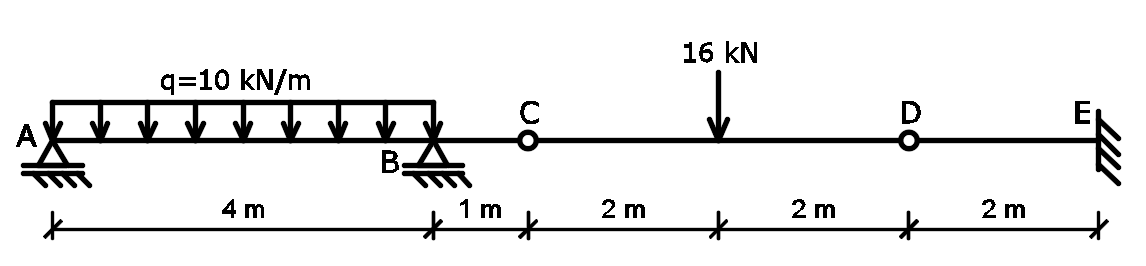
\includegraphics[width=0.85\textwidth]{pracEj1}
\end{center}
%
\noindent
Se pide:

\parte demostrar que la estructura es isostática, calcular las reacciones, y trazar los diagramas de solicitaciones;
\parte dimensionar la sección considerando que $b$ debe ser múltiplo de $5$;
\parte bosquejar la deformada de la estructura y calcular los giros en los apoyos A y B, junto con el desplazamiento vertical en C, suponiendo que la rigidez flexional $EI$ es uniforme y que $E =10$ GPa.



% ----------------------------
\ejercicio
%
Considere la estructura mostrada en la figura.
%
\begin{center}
	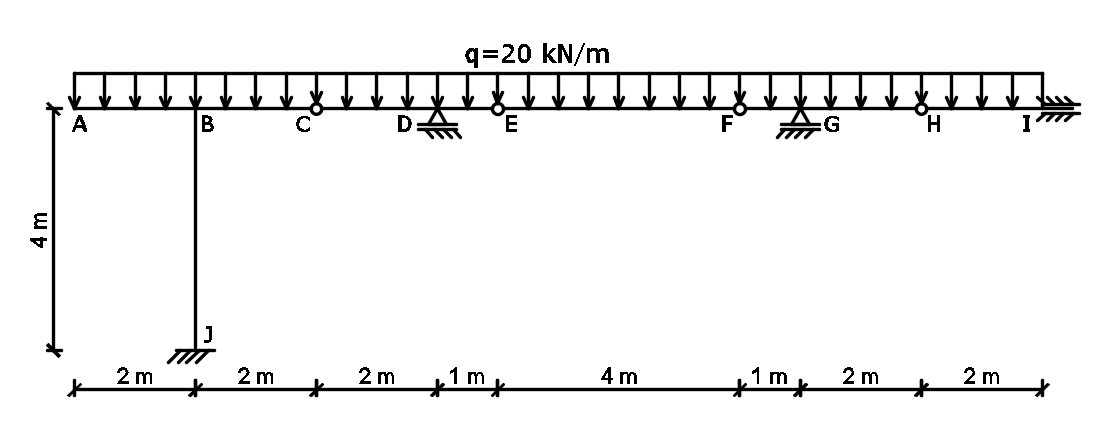
\includegraphics[width=\textwidth]{pracEj2}
\end{center}
%
\noindent
Se pide:
\parte Calcular las reacciones y trazar los diagramas de solicitaciones.
\parte Bosquejar la deformada de la estructura.
\parte Calcular los giros sobre los apoyos y los desplazamientos de C y H considerando $EI$ uniforme y despreciando la deformación por directa.


% ----------------------------
\ejercicio
%
Considere la estructura mostrada en la figura.
%
\begin{center}
	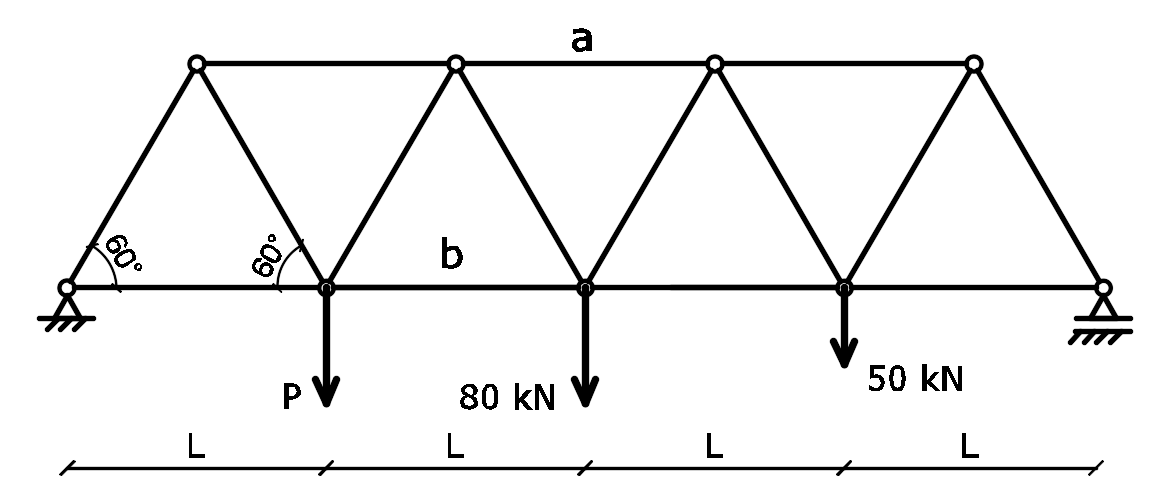
\includegraphics[width=0.85\textwidth]{pracEj3}
\end{center}
%
\noindent
Se pide:
\parte Obtener analíticamente los valores de la carga $P$ para los cuales la directa en la barra $a$ es igual en valor absoluto a la directa en la barra $b$.
\parte Verificar el resultado de la parte anterior utilizando alguna herramienta informática.
\parte Para el valor de $P$ positivo obtenido en a), dimensionar una sección transversal formada por 2 perfiles PNC a colocar en todas las barras de la estructura por igual, considerando que $\sigma_{adm} =140$ MPa.
%
%


\ejercicio
%
Considere la estructura mostrada en la figura, donde la carga dibujada con un círculo representa una carga movil unitaria.
%
\begin{center}
	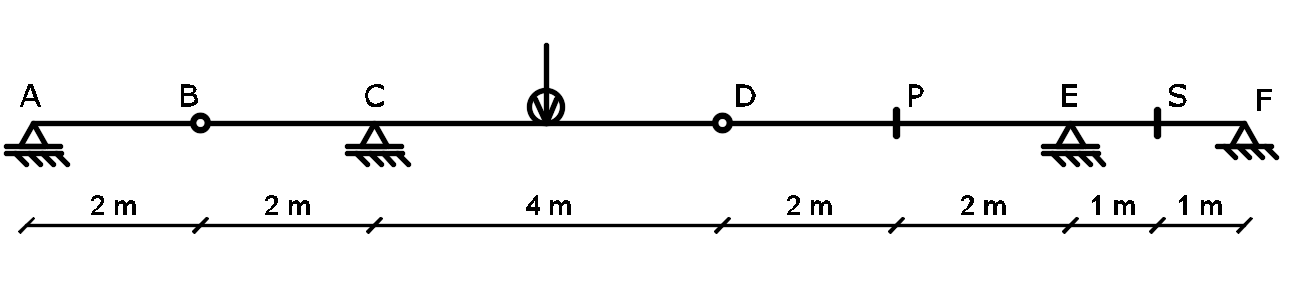
\includegraphics[width=\textwidth]{pracEj4}
\end{center}
%
\noindent
Se pide:
\parte Dibujar las líneas de influencia de la reacción en el apoyo C, del cortante en P y del momento flector en S para la estructura.
\parte Indicar dónde se debe colocar la carga uniforme $q=20$ kN/m para que RC, VP y MS sean máximos y mínimos. Encontrar dichos valores.
%



\ejercicio
Considere la estructura mostrada en la figura.
%
\begin{center}
	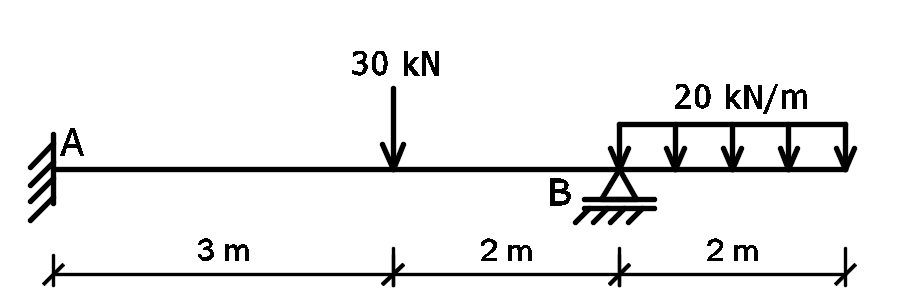
\includegraphics[width=0.6\textwidth]{pracEj5}
\end{center}
%
\noindent
Se pide:
\parte Calcular las reacciones y trazar diagramas de solicitaciones (EI=cte) aplicando el método de las ecuaciones angulares. 
\parte Verificar el resultado de la parte a) utilizando alguna herramienta informática.


% codigoFuenteLibroR2
% Copyright (C) 2020  J.M. Perez Zerpa, et. al.
%
% This program is free software: you can redistribute it and/or modify
% it under the terms of the GNU General Public License as published by
% the Free Software Foundation version 3 of the License.
%
% This program is distributed in the hope that it will be useful,
% but WITHOUT ANY WARRANTY; without even the implied warranty of
% MERCHANTABILITY or FITNESS FOR A PARTICULAR PURPOSE. See the
% GNU General Public License for more details.
%
% You should have received a copy of the GNU General Public License
% along with this program.  If not, see <http://www.gnu.org/licenses/>.

\chapter[Métodos energéticos aplicados a reticulados]{Métodos energéticos aplicados a reticulados}

En esta unidad temática se presentan los conceptos básicos necesarios para abordar el Método de los Desplazamientos (MD) y el Método de las Fuerzas (MF), en ambos casos, aplicados al análisis de estructuras reticuladas. %
%
Se comienza presentando los conceptos de indeterminación cinemática e indeterminación estática  para reticulados planos. %
%
Luego se presenta brevemente el Método de los desplazamientos y finalmente, para realizar el desarrollo del Método de las Fuerzas, se toma como referencias principal \citep{Reddy2002b}.


\section{Grados de indeterminación}

Existen diversos métodos disponibles para el análisis de una estructura, por lo tanto, es útil identificar qué tipo de métodos son los más adecuados \textit{antes} de iniciar el análisis estructural. %
%
En esta sección se presentan propiedades geométricas que pueden ser calculadas \textit{antes} del análisis, para, de esta forma, tomar una mejor decisión sobre el método a utilizar.

Los grados de indeterminación estática y cinemática son valores dados por la geometría y los vínculos existentes entre componentes de la estructura. %
%
Estos valores numéricos permiten estimar la complejidad de la resolución usando dos métodos analíticos presentados el curso: el \textit{Método de las Fuerzas} y el \textit{Método de los Desplazamientos}. %
%


\subsection{Grado de indeterminación cinemática}

El grado de indeterminación cinemática permite establecer la cantidad de incógnitas cinemáticas que se deben determinar para conocer el desplazamiento de todos los puntos de la estructura.
%
Una posible expresión matemática de este parámetro es:
%
\begin{equation}
	gk = g_l \, n_N - c_a,
\end{equation}
%
donde $g_l$ es el número de grados de libertad por nodo, $n_N$ es el número de nodos de la estructura y $c_a$ el número de grados de libertad conocidos por las condiciones de apoyo o vínculo a tierra. %
%
En estructuras articuladas planas $g_l$ es 2, en estructuras aporticadas planas $g_l=3$ y en aporticadas tridimensionales $g_l=6$.

El grado de indeterminación cinemática permite conocer el número de incógnitas de los sistemas de ecuaciones planteados al usar el Método de los Desplazamientos o sus variantes computacionales como el Método de los Elementos Finitos.

En el caso de la estructura mostrada en la Figura~\ref{fig:retic_gh}, se puede ver que $gk=2\times 4 - 4=4$.


\subsection{Grado de indeterminación estática}

% -------------------------
El grado de indeterminación estática (también llamado \textit{grado de hiperestaticidad}) es un valor numérico definido por la diferencia entre: el número de incógnitas de fuerza y el número de ecuaciones de equilibrio. %
%

\subsubsection{Grado de hiperestaticidad de reticulados}

En el caso particular de reticulados planos es posible obtener una forma simplificada de cálculo. %
% 
El estado tensional de las estructuras formadas por barras articuladas queda definido a partir de los valores de tensiones axiales o las directas de las barras (una incógnita por barra), y por las reacciones en cada uno de los vínculos a tierra. %
%
Cada barra introduce una directa como incógnita, mientras que cada componente de fuerzas de reacción también debe ser considerado (una incógnita por cada dirección).

Para las ecuaciones de equilibrio, en problemas planos, se cuenta con dos ecuaciones de equilibrio por cada nodo (cuerpo libre), por lo que el grado de hiperestaticidad puede ser escrito como
%
\begin{equation}
	\boxed{
	gh = n_R + n_{B} - 2 \times n_{N}
}
\end{equation}
%
donde $n_R$ es el número de reacciones a determinar, $n_B$ es el número de barras de la estructura y $n_N$ es el número de nodos.

En la estructura de la Figura~\ref{fig:retic_gh} se puede ver un reticulado formado por 6 barras con dos apoyos fijos. Se tienen $n_B=6$ solicitaciones por tener 6 barras, y $n_R=4$ por tener 2 reacciones en cada nodo apoyado fijo. %

\begin{figure}[htb]
	\centering
	\def\svgwidth{0.5\textwidth}
	\input{figs/UT1/retic_gh.pdf_tex}
	\caption{Ejemplo reticulado plano hiperestático.}
	\label{fig:retic_gh}
\end{figure}

Por otra parte, si se considera cada nodo de la estructura como un componente aislado se pueden plantear dos ecuaciones de equilibrio de fuerzas a cada componente, por lo tanto se tiene:
%
\begin{equation}
	gh = 4 + 6 - 2 \times 4 = 2.
\end{equation}

Tener una estructura con grado de hiperestacidad 2, es equivalente a decir que si se aplican las ecuaciones de equilibrio únicamente, tendríamos un sistema \textbf{compatible indeterminado}. El subespacio de soluciones del sistema será de dimensión 2.




\subsubsection{Clasificación de estructuras según grado de hiperestaticidad} %

Las estructuras pueden ser clasificadas según su grado de hiperestaticidad de la siguiente manera:

\begin{itemize}
	\item \textit{estáticamente determinada} (o isostática): es aquella estructura cuyo estado tensional puede ser determinado usando únicamente ecuaciones de equilibrio, por lo tanto:
	$$
	gh = 0
	$$
	
	\item \textit{hiperestáticas}: es aquella estructura para la cual no es posible determinar el estado tensional usando únicamente equilibrio, es decir:
	$$
	gh > 0.
	$$
	En este caso deben ser utilizadas oras ecuaciones como por ejemplo compatibilidad de desplazamientos. %
	
	\item \textit{hipoestáticas} (o mecanismos): este último caso corresponde a estructuras en las cuales se tienen más ecuaciones que incógnitas por lo tanto
	$$
	gh <0.
	$$
\end{itemize}




\subsubsection{Grado de hiperestaticidad externa}
%
Si la estructura puede ser considerada como un conjunto (sin mecanismos internos)  es posible definir el concepto de grado de hiperestaticidad externa como:
%
\begin{equation}
	gh_E = n_{R} - 3
\end{equation}
%
donde $n_R$ es nuevamente el número de reacciones. %
%

Finalmente, se puede usar los valores $gh_E$ y $gh$ para formular una condición \textbf{necesaria} que una estructura \textit{isostática} debe cumplir. %
%
Se dice que:
%
$$
\boxed{
	\text{Estructura isostática} \quad \Rightarrow \quad gh_E = 0 \quad \textbf{y} \quad gh = 0.
}%
$$
% -------------------------


%Existen casos de particulares, de estructuras en las cuales aún siendo isostáticas el grado de hiperestaticidad externa es mayor que cero, como por ejemplo la mostrada en la Figura~\ref{fig:hipereje}. %
%%
%Esto se debe a que la estructura está conformada por barras no conectadas entre sí como ocurre en la mostrada en las Figuras \ref{fig:ejemghMed} o \ref{fig:retic_gh}. %
%%
%Esta peculiaridad teórica no será relevante al momento de aplicación práctica del Método de las Fuerzas como se verá en la UT siguiente.





\subsubsection{Grado de hiperestaticidad para estructuras aporticadas}

Al considerar estructuras aporticadas, las ecuaciones deben ser modificadas y la complejidad en el cálculo aumenta. Este tipo de cálculo de $gh$ puede ser necesario si el Ingeniero analista cuenta con el Método de las Fuerzas como una de las opciones a aplicar en su análisis. Los estudiantes interesados en los métodos más generales de cálculo pueden consultar referencias como \citep{CerveraRuiz2002ii}. %
%


%En esta metodología se parte de un EBC, opcionalmente se pueden considerar componentes separadas de la estructura y se aplica una ecuación para el cálculo.
%
%Las \textbf{incógnitas de fuerza} son aquellas necesarias para determinar completamente el \textit{\textbf{estado tensional}} de toda la estructura. En las estructuras consideradas en este texto, estas incógnitas son:
%%
%\begin{itemize}
%	\item $n_S$: solicitaciones a determinar y fuerzas debidas a \textit{vínculos internos} de cada componente,
%	\item $n_R$: reacciones dadas por \textit{vínculos externos}.
%\end{itemize}
%
%
%Por otra parte para calcular el número de ecuaciones con que se cuenta se define:
%%
%\begin{itemize}
%	\item $n_C$: es el número de componentes o partes en la que se separa la estructura para el cálculo,
%	\item $n_E$: el número de ecuaciones de equilibrio para cada parte.
%\end{itemize}
%
%La expresión matemática del grado de indeterminación estática puede ser presentada como:
%%
%\begin{equation} \label{eqn:gradoh}
%	gh = n_R + n_S - n_C \, n_{E}.
%\end{equation}
%
%Como ejemplo se presentan las estructuras de la Figura~\ref{fig:ejemghSimp}, formadas por un único componente y con diferente cantidad de reacciones externas. Dado que no se cortan o liberan vínculos internos de la estructura no hay $n_S$.
%
%\begin{figure}[htb]
%	\centering
%	\def\svgwidth{0.95\textwidth}
%	\input{figs/UT1/ejemplos_basicosGradoHiper.pdf_tex}
%	\caption{Ejemplos simples de cálculo de grado de hiperestaticidad.}
%	\label{fig:ejemghSimp}
%\end{figure}
%
%En la Figura~\ref{fig:ejemghMed}. se muestra un reticulado, donde nuevamente si se desacopla en $n_C=3$ componentes una por barra, se tiene que cada articulación introduce dos vínculos a determinar. Por lo tanto $gh = 2+1+2+2+2-3\times 3 = 0$.
%
%\begin{figure}[htb]
%	\centering
%	\def\svgwidth{0.6\textwidth}
%	\input{figs/UT1/ejemplos_mediosGradoHiper.pdf_tex}
%	\caption{Ejemplo de cálculo de grado de hiperestaticidad en reticulado.}
%	\label{fig:ejemghMed}
%\end{figure}
%
%Este cálculo también puede ser realizado considerando la estructura como una única componente. Más adelante se mostrará una ecuación práctica para el cálculo de $gh$ en reticulados planos.
%
%\paragraph{Analogía con cálculo a partir de grados de libertad} %
%El cálculo presentado es análogo al utilizado en otros cursos, en los cuales se considera el número de grados de libertad total de las estructuras (en el ejemplo $3\times 3$) y se van restando los vínculos que restringen el movimiento entre barras y a tierra ($-2-1-2-2-2$) por lo que se obtiene un valor opuesto al $gh$.
%
%
%
%
%
%
%
%
%\subsubsection{Cálculo general de grado de hiperestaticidad en pórticos/vigas/barras planos}
%
%En el caso de estructuras de pórticos planos, la determinación del estado tensional requiere conocer 3 solicitaciones en todo punto: directa, cortante y momento. %
%%
%A modo de ejemplo se considera la estructura mostrada en la Figura~\ref{fig:gerb}: en la parte superior se muestra el esquema básico con la carga aplicada, mientras que en la parte inferior se muestra una de las formas en que la estructura puede ser separada en componentes. 
%%
%\begin{figure}[htb]
%	\centering
%	%
%	\def\svgwidth{0.7\textwidth}
%	\input{figs/UT1/ejemplo_grado_hiper.pdf_tex}
%	%
%	\caption{Ejemplo de grado de indeterminación estática: estructura con cargas aplicadas (superior) y estructura con componentes separadas y cantidad de reacciones incógnita (inferior).}
%	\label{fig:gerb}
%\end{figure}
%
%La cantidad de solicitaciones a determinar en cada vínculo es indicado con un círculo y el cálculo del grado de hiperestaticidad usando la Ecuación~\eqref{eqn:gradoh} está dado por:
%%
%\begin{equation}
%	n_R = 3+1+1 \quad n_S = 2+2 \quad n_C = 3 \quad n_E = 3 \quad \Rightarrow \quad gh = 0
%\end{equation}
%%
%por lo tanto la estructura es isostática.
%
%El $gh$ es un parámetro útil para estimar la complejidad de la aplicación del Método de las Fuerzas. %
%%
%Dado que en este texto dicho método es desarrollado únicamente para reticulados, el cálculo del $gh$ para pórticos no es abordado de forma extensiva. %
%%
%En la Sección 1.6 de \citep{CerveraRuiz2002ii} se presenta un desarrollo más extenso sobre la determinación del grado de hiperestaticidad así como también se muestran diversos ejemplos.
%
%
%





\section{Método de los Desplazamientos}

El desarrollo presentado en esta sección está enfocado a la versión matricial del MD para elementos de barra de dos nodos sin fuerzas de volumen y de sección transversal uniforme. %
%

Al desarrollar métodos de análisis de estructuras se utilizan hipótesis vinculadas al desplazamiento de los distintos elementos estructurales. %
De forma general se puede decir que los desplazamientos de todos los puntos de una estructura están dados por una suma de funciones de interpolación $\phi_i$ multiplicadas por los desplazamientos de los nodos de referencia de la estructura $u_i$:
%
\begin{equation}
u(P) = \sum_{i=1}^{n_d} u_i \phi_i(P),
\end{equation}
%
donde $P$ representa un punto cualquiera de la estructura y $n_d$ es el número de desplazamientos de referencia de la estructura (o número de incógnitas cinemáticas). %


El vector de todos los desplazamientos de referencia $\bfu \in \bbR^{n_d}$ brinda toda la información necesaria para construir la función de desplazamiento de toda la estructura (con el grado de aproximación brindado por las funciones $\phi$). %
%
Las funciones $\phi$ pueden ser tales que el desplazamiento de cada punto es una combinación lineal de los desplazamientos de los nodos extremos correspondientes.

Como ejemplo se considera el reticulado mostrado en la Figura~\ref{fig:retic_gh} se puede considerar que el desplazamiento de cualquier punto de las barras puede ser interpolado a partir de los desplazamientos de los nodos, por lo que se tendrían $8$ desplazamientos de referencia (dos por nodo).

Por otra parte, en cada nodo donde se definen desplazamientos de referencia $u_i$ se pueden considerar fuerzas externas aplicadas $f_i$.

\subsection{Interpolación lineal de desplazamientos}

En el caso de estructuras de barras articuladas, las funciones de interpolación pueden ser consideradas lineales en el dominio correspondiente a cada barra, siendo los desplazamientos de los nodos articulados los desplazamientos de referencia. %
%
Esto puede ser escrito para cada barra $e$ de la estructura usando las funciones lineales de interpolación:
%
\begin{equation}
\bfu (x^e) = \bfN^e(x^e) \bfu^e,
\end{equation}
%
donde $x^e$ es una coordenada local del elemento, $\bfN^e$ es la matriz de funciones de interpolación de la barra y $\bfu^e$ es el vector columna de los desplazamientos de los nodos de la barra. %
%


Se considera ahora elementos de barra como el mostrado en la Figura~\ref{fig:eleplabar} para los cuales sus movimientos están incluidos en un plano $x-y$. %
%
\begin{figure}[htb]
	\centering
  \def\svgwidth{0.6\textwidth}
  \input{figs/UT2/sistcord.pdf_tex}
	\caption{Esquema de sistemas de coordenadas de elemento de barra en el plano.}
	\label{fig:eleplabar}
\end{figure}

El desplazamiento según el eje de la barra, coincidente con el eje de coordenadas $x$ local, está dado por:
%
\begin{equation}
u_L^e(x^e) = N_1^e(x^e) u_{1,L}^e  + N_2^e(x^e) u_{2,L}^e,
\end{equation}
%
donde las funciones de interpolación están dadas por
%
\begin{equation}
N_1^e(x^e) = \frac{\ell^e - x^e}{\ell^e}
\quad \text{y} \quad N_2^e(x^e) = \frac{x^e}{\ell^e},
\end{equation}
%
siendo $\ell^e$ el largo de la barra $e$.


%
Usando la relación de deformación-desplazamiento y derivando (respecto a la coordenada local) se obtiene la expresión de la deformación en el dominio del elemento:
%
\begin{equation}
\varepsilon^e(x^e) = \frac{\partial u^e_L}{\partial x^e}(x^e) =  B_{1,L}^e(x^e) u_{1,L}^e  + B_{2,L}^e(x^e) u_{2,L}^e
\end{equation}
%
donde 
\begin{equation}
B_{1,L}^e(x^e) = \frac{- 1}{\ell^e}
\quad \text{y} \quad B_{2,L}^e(x^e) = \frac{1}{\ell^e},
\end{equation}
son las derivadas de las funciones de interpolación respecto a la coordenada local. %
%
Se observa que, para esta interpolación, la deformación axial es uniforme en todo el elemento (es decir que no depende de $x^e$) y vale 
%
\begin{equation}
\varepsilon^e  =  \frac{ u_{2,L}^e - u_{1,L}^e } {\ell^e}.
\end{equation}


Esto puede ser escrito en forma matricial como:
%
\begin{equation} \label{eqn:expreps}
\varep^e (\bfu^e_L) = \bfB_L^e \bfu^e_L,
\end{equation}
%
donde,
%
\begin{equation}
\bfB_L^e = \frac{1}{\ell^e} \left[-1, 0, 1, 0\right]
\quad \text{y} \quad
\bfu_L^e = \left[u_{1,L}, v_{1,L}, u_{2,L}, v_{2,L}\right]^T.
\end{equation}

Usando la ecuación constitutiva lineal se obtiene la tensión de cada elemento como:
%
\begin{equation}\label{eqn:barraeccons}
\sigma^e = E^e \varepsilon^e,
\end{equation}
donde $E^e$ es el módulo de Young del elemento o barra $e$ y $\sigma^e$ es la tensión axial, también uniforme en el elemento.


\subsection{Energía potencial total}

Para poder aplicar esta interpolación a los principios energéticos es necesario obtener una expresión de la energía potencial total de la estructura en función de los desplazamientos nodales. %
%
Para esto se sustituyen las expresiones obtenidas en las definiciones de la energía potencial de deformación elástica $\Pi_{int}$ y la energía potencial de las fuerzas externas $\Pi_{ext}$.

La energía potencial de deformación de cada barra está dada únicamente por la componente axial. Usando la expresión general dada por la Ecuación~\eqref{eqn:energbarra} y la forma del tensor de deformación dada por la Ecuación~\eqref{eqn:epsbarras}, se obtiene:
%
\begin{equation}
\Pi_{int}^e (\bfu_L^e) %
%
= \frac{1}{2} \int_{\Omega^e} E^e \left(\varepsilon^e (\bfu_L^e) \right)^2 \dif V ,
%
\end{equation}
%
donde $\Omega^e$ representa el volumen ocupado por la barra $e$. %
%
Sustituyendo la relación de la Ecuación~\eqref{eqn:expreps} y operando se obtiene:
%
\begin{equation}
\Pi_{int}^e(\bfu_L^e) = \frac{1}{2} (\bfu_L^e)^T \bfK_L^e \bfu_L^e ,
\end{equation}
%
donde $\bfK_L^e$ es una matriz dada por:
%
\begin{equation}\label{eqn:defK}
 \bfK_L^e = \int_{0}^{\ell^e} (\bfB_L^e)^T E^e A^e \bfB_L^e \dif x.
\end{equation}
%
La expresión desarrollada es:
%
\begin{equation}
\bfK_L^e = \frac{E^e A^e}{\ell^e} 
\left[
\begin{matrix}
1 & 0 & -1 & 0 \\
0 & 0 & 0 & 0\\
-1 & 0 &  1 & 0\\
0 & 0 & 0 & 0
\end{matrix}
\right].
\end{equation}
%

Para poder resolver problemas con varios elementos de barra, con sus ejes orientados en diferentes direcciones, es necesario trabajar con un sistema de coordenadas global. %
%
Considerando que el sistema de coordenadas local del elemento forma un ángulo $\alpha^e$ como se muestra en la Figura~\ref{fig:eleplabar} (medido antihorario desde el sistema global), la matriz de cambio de base $\bfR^e$ está dada por:
%
\begin{equation}\label{eqn:rotabarra}
\bfR^e = 
\left[
\begin{matrix}
c & -s & 0 & 0 \\
s & c & 0 & 0\\
0 & 0 &  c & -s\\
0 & 0 & s & c
\end{matrix}
\right]
\qquad
\bfu^e = \bfR^e \bfu^e_L
\end{equation}
%
donde $c=\cos(\alpha^e)$ y $s=\sin(\alpha^e)$ y $\bfu^e$ es el vector de desplazamientos del elemento en coordenadas globales. %
%

\cajaactividad{
Demostrar la identidad dada por la Ecuación~\ref{eqn:rotabarra} aplicando la relación de cambio de base vista en cursos de Álgebra Lineal:
$$
\text{coord}_B(\bfu) = 
_B(\bfI)_A
\text{coord}_A(\bfu),
$$
y la definición de matriz asociada de una transformación lineal.
}

Sustituyendo este cambio de coordenadas en la expresión de la energía potencial de deformación se tiene
\begin{equation}
\Pi_{int}^e(\bfu^e) = \frac{1}{2} (\bfu^e)^T \bfK^e \bfu^e,
\end{equation}
%
donde la matriz $\bfK^e$ en coordenadas globales está dada por:
%
\begin{equation}
\bfK^e = \bfR^e \bfK^e_L (\bfR^e)^T
= 
\frac{E^e A^e}{\ell^e}
\left[
\begin{matrix}
c^2 & cs & -c^2 & -cs \\
cs & s^2 & -cs & -s^2\\
-c^2 & -cs &  c^2 & cs\\
-cs & -s^2 & cs & s^2
\end{matrix}
\right].
\end{equation}




La energía potencial de deformación de toda la estructura puede ser calculada sumando las energías de las $n_e$ barras que forman la estructura:
%
\begin{equation}\label{eqn:matU}
  \Pi_{int}(\bfu) = \sum_{e=1}^{n_e} \Pi_{int}^e(\bfu^e) = 
   \sum_{e=1}^{n_e} \frac{1}{2} (\bfu^e)^T \bfK^e \bfu^e 
= \frac{1}{2} \bfu^T \bfK \bfu
\end{equation}
%
donde $\bfK$ es la versión \textit{ensamblada} de las matrices $\bfK$ y $\bfu$ es el vector de todos los deplazamientos nodales de la estructura.



Las fuerzas externas aplicadas son representadas por el vector $\bff_{ext}$ o simplemente $\bff$. %
%
La energía potencial de estas fuerzas es representada por $\Pi_{ext}$ y está dada por:
%
\begin{equation}
 \Pi_{ext}(\bfu) = - \sum_{i=1}^{n_d} u_i f_i = - \bfu^T \bff .
\end{equation}
%

La energía potencial total estará dada por lo tanto, por la suma de ambas energías:
%
\begin{equation}
\boxed{
\Pi(\bfu) = \frac{1}{2} \bfu^T \bfK \bfu - \bfu^T \bff .
}
\end{equation}



\subsection{Desarrollo del método}

Los principios energéticos brevemente descritos en la Unidad Temática 1 pueden ser revisados nuevamente en el contexto de estructuras de barras articuladas.


\subsubsection{Mínima energía potencial total}

Dada una estructura con condiciones de desplazamiento impuesto en un cierto conjunto de nodos, se establece que $\mcU$ es el conjunto de los desplazamientos compatibles con las condiciones de contorno. %
%


Considerando un cierto conjunto de cargas externas nodales dadas por el vector $\bff$, el Principio de mínima energía potencial establece que: entre todos los desplazamientos compatibles $\bfv \in \mcU$, los desplazamientos que están en equilibrio con las fuerzas externas son aquellos que verifican:
%
\begin{equation}
\bfu = \arg\min_{\bfv \in \, \mcU} \Pi(\bfv).
\end{equation}

Si las condiciones de contorno son tales que no se permiten movimientos rígidos de la estructura, entonces el desplazamiento solución será único.


\subsubsection{Primer teorema de Castigliano}

Utilizando la expresión de la energía potencial de las fuerzas externas y planteando las condiciones de optimalidad de primer orden del problema de minimización se obtiene:
%
\begin{equation}\label{eqn:castiguno}
\left\{ 
\begin{array}{l}
\displaystyle  \frac{\partial \Pi_{int} }{ \partial u_i}(\bfu) = f_i \qquad \forall i=1,\dots, n_d\\
  \bfu \in \mcU
\end{array}
  \right.
\end{equation}

Este conjunto de condiciones o ecuaciones representa el Primer Teorema de Castigliano. %
%





\subsubsection{ Ecuación de rigidez }

Sustituyendo la expresión matricial $\Pi_{int}$ de la Ecuación~\eqref{eqn:matU} en las condiciones del Teorema de Castigliano dadas por la Ecuación~\eqref{eqn:castiguno}, se obtiene el siguiente sistema de ecuaciones lineales:
%
\begin{equation}
\boxed{
	\bfK \bfu = \bff
},
\end{equation}
%
el cual acompañado de las condiciones de contorno representan el sistema a formar y resolver para aplicar el Método de los Desplazamientos en su forma matricial. %

La matriz $\bfK$ es llamada \textbf{matriz de rigidez} global de la estructura ya que vincula desplazamientos con fuerzas aplicadas. %
%
Es importante destacar que la cantidad de incógnitas del sistema es igual al grado de indeterminación cinemática $gk$ introducido en la Unidad Temática 1.

	\subsubsection{Cálculo de solicitaciones}

Las solicitaciones de interés en el análisis de reticulados son las fuerzas directa $N^e$ en cada elemento de barra
%
\begin{equation}
N^e = \sigma^e A^e.
\end{equation}
%
Para ello se pueden utilizar las ecuaciones \eqref{eqn:epsbarras}, \eqref{eqn:barraeccons} y \eqref{eqn:rotabarra}:
%
\begin{equation}\label{eqn:expSolic}
N^e = E^e A^e \bfB_L^e (\bfR^e)^T \bfu^e.
\end{equation}


Finalmente se menciona que también es posible analizar reticulados con resortes elásticos en sus nodos. Para esto se puede adicionar a las ecuaciones los correspondientes términos de energía potencial elástica. %
%
En el caso de un resorte lineal de constante elástica $k$ colocado en el grado de libertad $j$, la energía potencial está dada por
%
\begin{equation}
\Pi_{res}(\bfu) = \frac{1}{2} k u_j^2,
\end{equation}
%
que puede ser sumada a la energía potencial de deformación $\Pi_{int}$.







\subsection{Implementación computacional}

Este método puede ser programado para resolver problemas de mayor dimensión de forma automática usando herramientas de cálculo numérico de alto nivel como GNU-Octave \citep{Eaton2015}, Python o Julia.  %

En el mismo repositorio en el que se encuentran los contenidos de este material, se puede encontrar una carpeta \textit{UT2} dentro de la carpeta \textit{octave}. Allí se puede explorar el archivo \textit{FEMTrusS.m} en el cual hay una implementación del método para reticulados planos


El objetivo del código es mostrar a los estudiantes la aplicación directa de los conceptos vistos, así como también permitir un espacio para el desarrollo propio incluyendo nuevas funcionalidades como por ejemplo la capacidad de resolver reticulados tridimensionales. %
%
Este código está en proceso de revisión por lo que, para la resolución de los ejercicios prácticos, se recomienda usar los otros programas recomendados en el curso. %
%
En caso de detectar errores se agradece notificarlo creando un \textit{issue}.




\subsection{Ejemplo de Método de los Desplazamientos} \label{sec:ejemplobarra}

Sea la estructura mostrada en la Figura~\ref{fig:ejejmMDUT2}, formada por barras de material con módulo de Young $E=210 $ GPa, con $\ell= 10$ m, y secciones transversales  de áreas $A^1 = A^3 = 0.001$ m$^2$ y $A^2 = 0.01 $ m$^2$. %
%
Para la fuerza aplicada $P= 10 $ kN, se desea determinar desplazamientos y solicitaciones de la estructura. Utilizando el método de los desplazamientos matricial.

\begin{figure}[htb]
\centering
\begin{center}
	\def\svgwidth{0.6\textwidth}
	\input{figs/UT2/ejRetic.pdf_tex}
\end{center}
\caption{Ejemplo Método de los Desplazamientos.}
\label{fig:ejejmMDUT2}
\end{figure}


El grado de indeterminación cinemática de la estructura es $gk = 2 \cdot 4 - 2 \cdot 3 = 2$. %
%
Se continúa determinando los grados de libertad correspondientes a cada elemento de barra. Se define la matriz de conectividad y se calculan los ángulos $\alpha^e$.
%
\begin{center}
	\begin{tabular}{cccc}
		\hline
		Elemento & nodo inicial $\rightarrow$ nodo final & grados de libertad & $\alpha^e$\\
		\hline
		1 & 1 $\rightarrow$ 2 & 1 2 3 4 & 45$^\circ$\\
		2 & 2 $\rightarrow$ 3 & 3 4 5 6 & -90$^\circ$\\
		3 & 2 $\rightarrow$ 4 & 3 4 7 8 & -45$^\circ$\\
		\hline
	\end{tabular}
\end{center}

Se calculan las matrices de rigidez en coordenadas globales:
\begin{equation}
\bfK^1 = \frac{ 210 \times10^9 \cdot 1 \times 10^{-3} }{ \sqrt{2}  \cdot 10} \frac{1}{2}
\left[
\begin{matrix}
1 & 1 & -1 & -1 \\
1 & 1 & -1 & -1\\
-1 & -1 &  1 & 1\\
-1 & -1 & 1 & 1
\end{matrix}
\right]
\text{N/m}
\end{equation}

Operando se tiene
\begin{equation}
\bfK^1 = 7.425 \times 10^6
\left[
\begin{matrix}
1 & 1 & -1 & -1 \\
1 & 1 & -1 & -1\\
-1 & -1 &  1 & 1\\
-1 & -1 & 1 & 1
\end{matrix}
\right]
\text{N/m}
\end{equation}

Para el elemento 2 se tiene
\begin{equation}
\bfK^2 = 210 \times 10^6
\left[
\begin{matrix}
0 & 0 & 0 & 0 \\
0 & 1 & 0 & -1\\
0 & 0 &  0 & 0\\
0 & -1 & 0 & 1
\end{matrix}
\right]
\text{N/m}
\end{equation}

Para el elemento 3 se tiene
\begin{equation}
\bfK^3 = 7.425 \times 10^6
\left[
\begin{matrix}
1 & -1 & -1 & 1 \\
-1 & 1 & 1 & -1\\
-1 & 1 &  1 & -1\\
1 & -1 & -1 & 1
\end{matrix}
\right]
\text{N/m}
\end{equation}



Se observa que el elemento 2 tiene una rigidez mayor (dada por su sección transversal) aunque esta rigidez solamente vincula los desplazamientos verticales de los nodos 2 y 3.

Considerando que los grados de libertad fijos o de desplazamiento nulo son 1, 2, 5, 6, 7 y 8 y ensamblando las matrices en los grados de libertad restantes (3 y 4) se tiene.
%
\begin{equation}
\bfK =
7.425 \times 10^6
\left[
\begin{matrix}
1 & 1 \\
1 & 1 
\end{matrix}
\right]
\text{N/m}
+
210 \times 10^6
\left[
\begin{matrix}
0 & 0 \\
0 & 1 
\end{matrix}
\right]
\text{N/m}
+
7.425 \times 10^6
\left[
\begin{matrix}
1 & -1 \\
-1 & 1 
\end{matrix}
\right]
\text{N/m}
\end{equation}


Se obtiene entonces el sistema de ecuaciones a resolver
\begin{equation}
\quad 10^6
\left[
\begin{matrix}
14.84 & 0 \\
0 & 224.84 
\end{matrix}
\right]
\text{N/m}
\,
\bfu = 
\left[
\begin{matrix}
10^4 \\
0 
\end{matrix}
\right] \text{N}.
\end{equation}
%
Cuya resolución brinda los desplazamientos solución:
%
\begin{equation}
\boxed{
	u_{2} = 6.74 \times 10^{-4} \text{m}  \qquad v_{2} = 0.
}\end{equation}

Ahora que están determinados los desplazamientos de todos los nodos de la estructura es posible determinar la directa $N^e$ en todas las barras usando la Ecuación~\eqref{eqn:expSolic}:
%
\begin{equation}
N^1 = - N^3 =7.07 \, \text{kN} \quad \text{y} \quad N^2 = 0.
\end{equation}


Las directas también pueden ser obtenidas usando la ecuación de rigidez para cada elemento de barra, dada por:
%
$$
\bfK^e \bfu^e = \bff^e.
$$


Los resultados obtenidos pueden ser verificados utilizando el código mencionado en la sección anterior. En la Figura~\ref{fig:ejbarraDef} se muestra el diagrama de deformada con factor de escala 1000.

\begin{figure}[htb!]
	\centering
	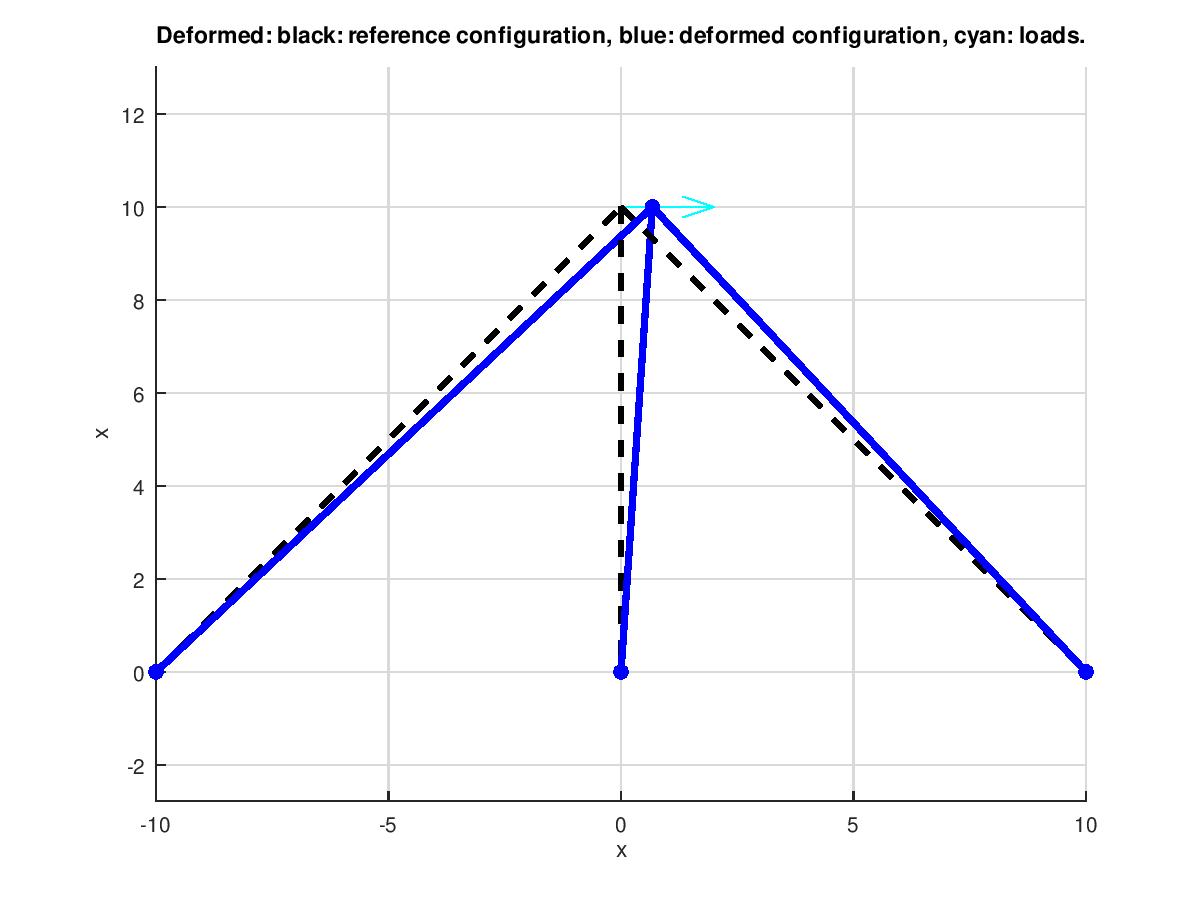
\includegraphics[width=0.65\textwidth]{deformed}
	\caption{Gráficos de deformada generado por el código FEMTrusS para el ejemplo presentado usando un factor de escala 1000.}
	\label{fig:ejbarraDef}
\end{figure}


En la Figura~\ref{fig:ejbarraDir} se muestra el diagrama de directas, también generado usando FEMTrusS.  %

\begin{figure}[htb!]
	\centering
	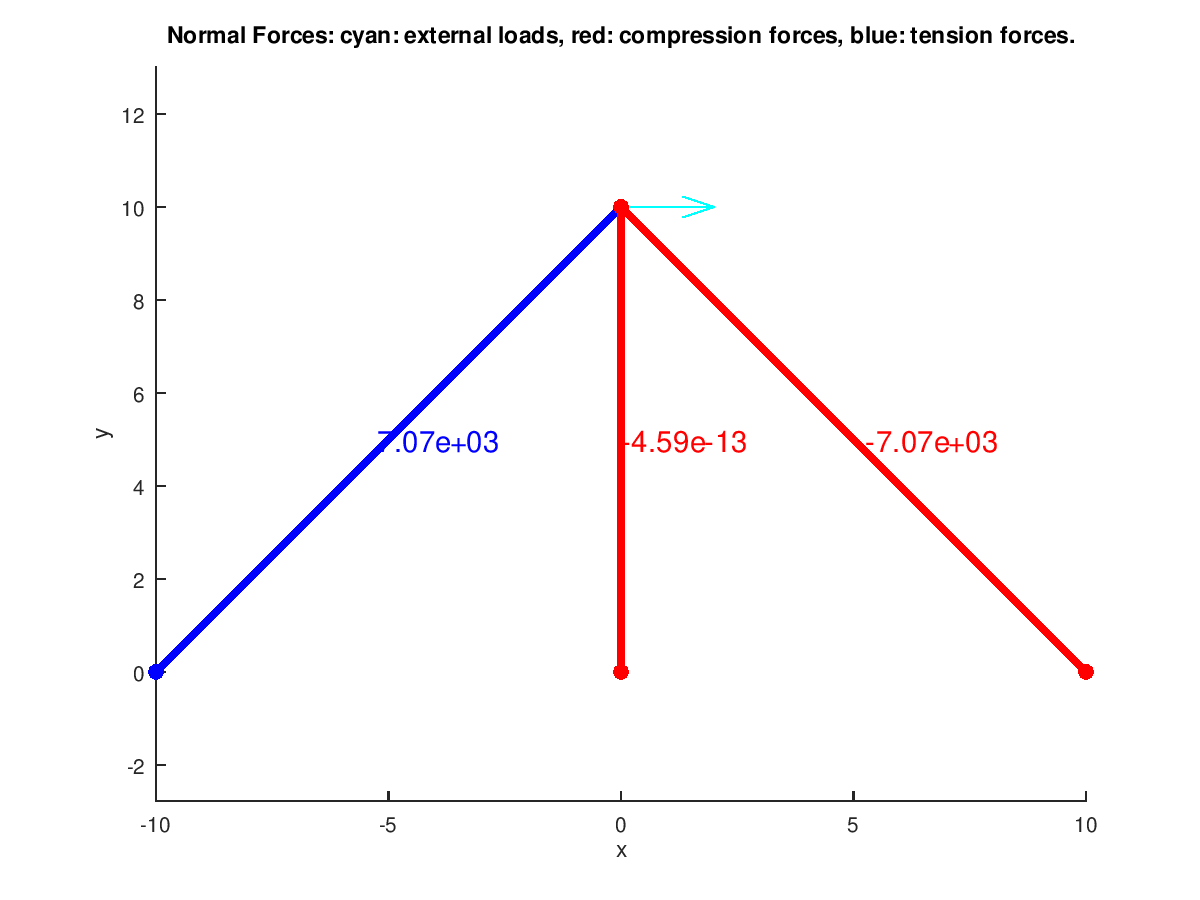
\includegraphics[width=0.65\textwidth]{normalforces}
	\caption{Gráficos de directas generado por el código FEMTrusS para el ejemplo presentado.}
	\label{fig:ejbarraDir}
\end{figure}



Finalmente, se menciona que si se considerara un resorte horizontal de constante elástica $k$ en el nodo 2 entonces se agregaría el término de energía potencial de deformación: $\frac{1}{2} k u_2^2$. %
%%
Luego de realizar las derivadas establecidas por Castigliano se obtendría $k u_2$, término que es considerado en el sistema lineal reducido como
%
\begin{equation}
\bfK =
\left[
\begin{matrix}
14.84 \times10^6 +k & 0 \\
0 & 224.84 \times10^6 
\end{matrix}
\right]
\end{equation}
%
lo cual resultaría en, como es esperado, un menor valor de desplazamiento nodal.




%%%%%%%%%%%%%%%%%%%%%%%%%%%%%%%%%%%%%%%%%%%%%%%%%%%%%%%%%%%%%%%%
%%%%%%%%%%%%%%%%%%%%%%%%%%%%%%%%%%%%%%%%%%%%%%%%%%%%%%%%%%%%%%%%
% metodo de las fuerzas
%%%%%%%%%%%%%%%%%%%%%%%%%%%%%%%%%%%%%%%%%%%%%%%%%%%%%%%%%%%%%%%%
%%%%%%%%%%%%%%%%%%%%%%%%%%%%%%%%%%%%%%%%%%%%%%%%%%%%%%%%%%%%%%%%
\section{Método de las Fuerzas}


El Método de las Fuerzas (MF) utiliza un enfoque de resolución complementario al MD. El MF considera las ecuaciones de equilibrio de fuerzas y tiene como objetivo primario determinar las incógnitas de fuerzas indeterminadas por esas ecuaciones. %
%
En el MD se utilizan principalmente ecuaciones constitutiva y de  compatibilidad cinemática, con el objetivo de obtener los desplazamientos.


En esta sección (y en el curso) se presenta el método orientado únicamente al análisis de reticulados, utilizando un enfoque similar al usado en \citep{Reddy2002b}. %
El MF puede ser aplicado al análisis de cualquier estructura hiperestática, los estudiantes interesados en la aplicación del MF a estructuras como pórticos pueden acudir a textos como \citep{Krenk2013,Fuchs2016} disponibles\footnote{Acceso variable año a año, definido por el financiamiento destinado a la ANII.} en la colección \textit{Springer} en \href{http://timbo.org.uy/}{timbo.org.uy}.
%


Tal como fue visto, los desplazamientos son la incógnita principal del MD. %
En el caso del MF los valores de las directas en las barras y las reacciones de los vínculos son la incógnita principal a determinar. %
%
Para ello se cuenta con las ecuaciones de equilibrio, condiciones de compatibilidad de desplazamientos y principios energéticos.


En el caso de estructuras isostáticas las ecuaciones de equilibrio permiten determinar el estado tensional y solicitaciones de la estructura de forma única, por lo que el MF no puede ser aplicado de forma directa. %
%
%
Nos enfocaremos en estructuras con grado de hiperestaticidad $gh$ positivo, para las cuales las directas $\textbf{N}$ y las reacciones $\textbf{R}$ que se encuentran en equilibrio con las fuerzas externas pueden ser calculadas como combinación de estados llamados canónicos. %

\cajaactividad{Enumerar las $9$ incógnitas de fuerzas (solicitaciones internas y reacciones) del Ejemplo de la Sección~\ref{sec:ejemplobarra}, aplicar las ecuaciones de equilibrio y despejar todas las incógnitas en función de la directa de la barra 3 ($N^3$). %
Escribir el conjunto de los vectores de $\bbR^9$ que cumplen el equilibrio como una suma de vectores dependientes de $P$ y $N^3$.}


\subsection{Estados Canónicos}

Los estados canónicos serán considerados como: estados tensionales que pueden ser combinados para obtener el estado tensional real de una estructura hiperestática. %
%
Estos estados canónicos pueden ser obtenidos liberando vínculos internos y/o externos de una estructura hiperestática original, hasta obtener una estructura isostática.

En la Figura~\ref{fig:estadoscanon} se muestra un ejemplo de una estructura hiperestática con $gh=2$, con un vínculo de hiperestaticidad interno y uno externo, por lo que se obtiene una estructura isostática ''cortando'' una barra y liberando un vínculo de uno de los apoyos. %


\begin{figure}[htb]
	\centering
	\def\svgwidth{0.95\textwidth}
\input{figs/UT2/MF.pdf_tex}
	\caption{Ejemplo de descomposición de estados canónicos para aplicación del MF.}
	\label{fig:estadoscanon}
\end{figure}

El estado fundamental $E_0$ corresponde a la estructura isostática resultante sometida a las fuerzas externas. %
%
El estado $E_1$ corresponde a la misma estructura isostática considerando dos fuerzas aplicadas en los extremos intermedios obtenidos luego del corte de la barra. Estas fuerzas unitarias consideradas corresponden a una directa unitaria en la barra cortada. %
%
En el estado $E_2$ se considera una fuerza horizontal correspondiente al vínculo liberado.
%
%Los valores de las fuerzas son multiplicados por un factor $X_1$.
% --------------------------------------



Se puede considerar que las fuerzas externas consideradas en la estructura son una combinación de las fuerzas externas correspondientes a cada estado canónico
%
\begin{equation}\label{eqn:fueX}
\bff(\bfX) = \bff_0 + \sum_{j=1}^{gh} X_j \bff_j,
\end{equation}
donde  $\bff_0$ representa el vector de fuerzas externas aplicadas a la estructura original, $\bff_j$ corresponde a las fuerzas de cada estado canónico y $\bfX$ es el vector de multiplicadores de cada estado.
%
En el ejemplo, $\bff_1$ corresponde a un vector con dos fuerzas unitarias colocadas en puntos muy cercanos dados por el corte de la barra (o bien en los nodos extremos de la barra cortada) y $\bff_2$ corresponde a un vector con la fuerza unitaria aplicada en el apoyo deslizante.

Por otra parte, las ecuaciones de equilibrio definen una relación entre directas y fuerzas externas. %
Esta relación entre directas de las barras y fuerzas externas aplicadas $N=N(\bff)$, donde las fuerzas externas de cada estado son conocidas. %
%
Usando la relación $\bff(\bfX))$ se puede obtener una expresión de directas considerando los factores $X_j$ como las incógnitas a determinar:
%
\begin{equation}\label{eqn:estadosdirectas}
\textbf{N}(\bfX) = \textbf{N}_0 + \sum_{j=1}^{gh} X_j \textbf{N}_j
\end{equation}
%
donde el subíndice $j$ representa los valores del estado $j$, $X_j$ representa un factor a determinar, $\bfN_0$ corresponde a las directas para el estado de cargas $\bff_0$ y $\bfN_j$ corresponde a las directas para el estado de cargas unitarias $\bff_j$.
%
% ------------


Esto mismo también es realizado para calcular las reacciones de la estructura:
%
\begin{equation}
\textbf{R}(\bfX) = \textbf{R}_0 + \sum_{j=1}^{gh} X_j \textbf{R}_j
\end{equation}

Si se considera que las directas $\bfN$ y las reacciones $\bfR$ son las incógnitas principales del método entonces, se puede decir que los estados canónicos permiten interpolar los posibles estados tensionales. Los estádos canónicos en el MF cumplen el rol de las funciones de interpolación de desplazamientos en el MD, mientras que los valores de las incógnitas $\bfX$ cumplen el rol de los desplazamientos nodales.

\subsection{Principios energéticos}

Hasta aquí se han presentado las fuerzas de los factores $X_j$ asociados a incógnitas de fuerza de los vínculos liberados del problema. %
%
Los valores de directas usados para calcular la energía de deformación complementaria, son obtenidos a partir de las relaciones directas-fuerzas externas del equilibrio de fuerzas. %
%
Se destaca que no se han tomado en consideración las condiciones cinemáticas establecidas por las condiciones de apoyo de la estructura, el principio de mínima energía potencial complementaria permite obtener condiciones para esto.


Para presentar el método de las fuerzas se deben introducir los conceptos de energía de potencial complementaria. %

\subsubsection{Energía potencial de deformación complementaria}
%
La energía potencial de deformación presentada $\Pi_{int}$ puede ser escrita en términos de las tensiones en lugar de los desplazamientos. %
%
Consideremos la energía de deformación de un elemento de barra:
%
\begin{equation}
\Pi_{int}^e(\bfu^e) = \frac{1}{2} \int_0^{\ell^e} \varep^e(\bfu^e) E^e A^e \varep^e(\bfu^e) dx
\end{equation}
%
usando la ecuación constitutiva se obtiene una expresión en función de la tensión del elemento
%
\begin{equation}
\Pi_{int}^e(\bfu^e) = \frac{1}{2} \int_0^{\ell^e} \sigma^e \sigma^e \frac{1}{E^e} A^e dx = (\Pi_{int}^*)^e(\sigma^e) 
\end{equation}
%
donde $\Pi_{int}^*$ representa la energía de deformación complementaria de la barra. %
%
En el caso de materiales elástico-lineales, como los considerados en este documento, la energía complementaria $\Pi_{int}^*$ coincide con la energía de deformación $\Pi_{int}$.
% ----------------------------

Usando que no hay fuerzas de volumen aplicadas a la barra y considerando la directa de la barra $N^e = \sigma^e A^e$ se obtiene una expresión de la energía en función de la directa:
%
\begin{equation}
(\Pi_{int}^*)^e(\bff) = \frac{1}{2} \frac{(N^e (\bff))^2}{E^e A^e} \ell^e.
\end{equation}
%
donde las fuerzas externas $\bff$ están relacionadas con la directas a través de las ecuaciones de equilibrio. %
%
La energía de deformación complementaria de la estructura completa está dada por la suma:
%
\begin{equation}\label{eqn:Udef}
\Pi_{int}^*(\bff) =  \frac{1}{2} \sum_{e=1}^{n_e} \frac{(N^e (\bff))^2}{E^e A^e} \ell^e.
\end{equation}

Para estructuras hiperestáticas, se puede considerar la relación entre $\bff$ y $\bfX$ y considerar el vector $\bfX$ como variable:
%
\begin{equation}
\boxed{
(\Pi_{int}^*)^e(\bfX) = \frac{1}{2} \frac{(N^e (\bfX))^2}{E^e A^e} \ell^e.
}
\end{equation}

\subsubsection{Energía potencial complementaria de cargas externas}
La energía potencial de las cargas externas $\Pi_{ext}$ puede ser considerada también como una función de las fuerzas externas aplicadas, de la forma:
%
\begin{equation}\label{eqn:Vdef}
\Pi_{ext}(\bfu) = -\bfu^T \bff = \Pi_{ext}^*(\bff).
\end{equation}





\subsubsection{Energía potencial complementaria total}

La energía potencial complementaria total puede también ser escrita en función de las variables $\bfX$. %
%
Sustituyendo la Ecuación~\eqref{eqn:estadosdirectas} en la definición de $\Pi_{int}^*$ (Ecuación~\eqref{eqn:Udef})  y la Ecuación~\eqref{eqn:fueX} en la definición de $\Pi_{ext}^*$ (Ecuación~\eqref{eqn:Vdef}) se obtiene:
%
\begin{equation}
\Pi^* (\bfX) = \frac{1}{2}  \sum_{e=1}^{n_e} \frac{(N_0^e + \sum_{j=1}^{gh} X_j N_j^e)^2}{E^e A^e} \ell^e - \bfu^T \bff_0 - \bfu^T \left( \sum_{j=1}^{gh} X_j \bff_j \right).
\end{equation}


\subsubsection{Mínima energía potencial complementaria total}

El principio de mínima energía potencial complementaria total establece que dada una estructura con ciertas condiciones de apoyos y un conjunto de fuerzas externas aplicadas, la distribución de fuerzas internas en equilibrio compatible con los vínculos de los desplazamientos es aquella que minimiza la energía potencial complementaria total de la estructura. Esto puede ser escrito en función de los factores $X_j$, de la forma:
%
\begin{equation}
\textbf{X} = \argmin_{\textbf{X} \in \bbR^{gh} } \Pi^*(\textbf{X}).
\end{equation}

\subsubsection{Segundo teorema de Castigliano}

El segundo Teorema de Castigliano consiste básicamente en las condiciones de optimalidad del problema de mínimo de energía potencial complementaria total, %
%
las cuales consisten en plantear gradiente nulo:
%
\begin{equation}
\frac{\partial \Pi^*}{ \partial X_i}(\bfX) = 0  \quad i=1,\dots,gh \Rightarrow 
\frac{\partial \Pi_{int}^*}{ \partial X_i}(\bfX) = \bfu^T \bff_i \quad i=1,\dots,gh.
\end{equation}
%
Considerando que los valores de fuerzas externas de los estados canónicos distintos al fundamental son unitarios se tiene:
%
\begin{equation}
\frac{\partial \Pi_{int}^*}{ \partial X_i}(\bfX) =  \delta_i \qquad i=1,\dots,gh
\end{equation}
%
donde $\delta_i$ representa el desplazamiento nodal (o la suma de varios desplazamientos) de la estructura como resultado de las cargas externas aplicadas en los puntos donde hay fuerzas unitarias aplicadas en el estado canónico $i$. %
%
Este desplazamiento deberá tomar un valor compatible con el vínculo que fue liberado. %

En los casos en los que el vínculo liberado está asociado a un desplazamiento nulo (continuidad o apoyos fijos) se tiene
%
\begin{equation}
\frac{\partial \Pi_{int}^*}{ \partial X_i}(\bfX) = 0 \qquad i=1,\dots,gh.
\end{equation}

En el ejemplo mostrado en la Figura~\ref{fig:estadoscanon}, para el estado 1 el desplazamiento corresponde a la resta de los desplazamientos de los nodos obtenidos luego del corte, lo cual, dado que hay continuidad, debe ser cero. %
%
Para el estado 2 el desplazamiento corresponde a cero ya que el vínculo liberado corresponde a un apoyo fijo. %
%


\subsection{Método de las Fuerzas para análisis de reticulados}

En esta sección se presentan esquemáticamente las ecuaciones del MF para el análisis de reticulados.


El método consiste en liberar $gh$ vínculos de la estructura para obtener una estructura isostática y aplicar las ecuaciones del segundo teorema de Castigliano, imponiendo el desplazamiento correspondiente a los vínculos liberados. %

En el caso de estructuras de barras articuladas donde los vínculos liberados tienen desplazamiento nulo, y aplicando el segundo teorema de Castigliano se tiene:
%
\begin{equation}
 \frac{\partial \Pi_{int}^*}{ \partial X_i}(\bfX) =  \sum_{e=1}^{n_e} \frac{N_i^e(N_0^e + \sum_{j=1}^{gh} X_j N_j^e)}{E^e A^e} \ell^e = 0
 \qquad i=1,\dots, gh
\end{equation}
%
donde se consideró que el desplazamiento de cada estado corresponde a un valor nulo. %

Desarrollando el producto se obtienen $gh$ condiciones
\begin{equation}
\sum_{j=1}^{gh}  X_j \left( \sum_{e=1}^{n_e}  \frac{ N_j^e N_i^e } {E^e A^e} \ell^e \right) = - \sum_{e=1}^{n_e} \frac{N_i^e N_0^e } {E^e A^e} \ell^e \qquad i=1,\dots,gh,
\end{equation}
%
lo que representa un sistema lineal de ecuaciones de $gh$ incógnitas y ecuaciones.
% ---------------------------


Escrito en forma matricial esto es:
\begin{equation}\label{eqn:ecflex}
\bfM_f \bfX = \bfb_f
\end{equation}
%
donde $\bfM_f$ es llamada matriz de flexibilidad y sus entradas están dadas por:
%
\begin{equation}
(\bfM_f)_{ij} =  \sum_{e=1}^{n_e} \frac{N_i^e N_j^e }{E^e A^e} \ell^e,
\end{equation}
y el término independiente $\bfb_f$ está dado por:
%
\begin{equation}
(\bfb_f)_{i} =  - \sum_{e=1}^{n_e} \frac{N_0^e N_i^e }{E^e A^e} \ell^e.
\end{equation}

La Ecuación~\eqref{eqn:ecflex} es llamada ecuación de flexibilidad.
	
\subsubsection{Procedimiento práctico de aplicación}

\begin{enumerate}
\item calcular el grado de hiperestaticidad de la estructura $gh$,
\item si $gh$ es positivo entonces liberar $gh$ vínculos de la estructura obteniendo $gh+1$ esquemas básicos de estructuras isostáticas (estados canónicos),
\item calcular las directas y reacciones para cada uno de los estados canónicos,
\item calcular la matriz de flexibilidad y el término independiente,
\item calcular los factores de cada estado $X_j$ resolviendo la ecuación de flexibilidad,
\item calcular los valores de directa y reacciones solución sustituyendo los valores $X_j$.
\end{enumerate}


\subsubsection{Cálculo de desplazamiento}

El segundo teorema de Castigliano puede ser aplicado también para calcular el desplazamiento de cualquier punto de la estructura. %
%
Dado un vector de fuerza $\bfX_{sol}$ obtenido como solución de la ecuación de flexibilidad, se considera un estado canónico adicional $E_{gh+1}$ con una fuerza externa unitaria según el desplazamiento deseado. %
%
Se aplica Castigliano y a través de la derivada de la energía respecto el valor correspondiente de $X$ y considerando que este valor $X$ debe ser nulo se obtiene el desplazamiento deseado. %
%
\begin{equation}
\delta_{gh+1} = \frac{\partial \Pi^*_{int}}  { \partial X_{gh+1} } (\bfX = \bfX_{sol}, X_{gh+1}=0)
\end{equation}

Existe un caso particular destacable. %
%
Si en el estado canónico $E_0$ existe una única fuerza aplicada de magnitud $P$, y además el estado canónico $E_{gh+1}$, necesario para calcular el desplazamiento, cumple que $E_0 = P E_{gh+1}$, entonces se puede probar que %
%
\begin{equation}
\delta_{gh+1} = \frac{\partial \Pi^*_{int}}  { \partial P } (\bfX = \bfX_{sol}, X_{gh+1}=0).
\end{equation}
%



\subsection{Implementación computacional}

La implementación computacional del procedimiento del Método de las Fuerzas no es tan directa como la del Método de los Desplazamientos. %
%
A pesar de esto, se brinda un ejemplo de implementación, que puede ser también estudiado por los estudiantes interesados en entender el procedimiento planteado por el método. %
%
Los códigos están disponibles en el repositorio \href{https://github.com/jorgepz/Force-Method-Solver}{github.com/jorgepz/Force-Method-Solver}, y se aclara que el código es una versión minimal, en proceso de revisión, que aspira simplemente a mostrar una posible forma de automatizar el proceso del Método y  no forma parte de los contenidos del curso. %
%



\subsection{Ejemplo de Método de las Fuerzas}

Se presenta la resolución del mismo problema de la Sección~\ref{sec:ejemplobarra}, en este caso usando el MF. %
%
Se comienza calculando el grado de hiperestaticidad como $gh= 3 + 6 - 2 \times 4 = 1$.


En este problema existen más de una posibilidad de estados canónicos a considerar. En la Figura~\ref{fig:hipereje} se muestran los estados canónicos elegidos, considerando un corte en la barra 2-4.

\begin{figure}[htb]
\centering
\def\svgwidth{\textwidth}
\input{figs/UT2/Ej_UT2_retic_MF.pdf_tex}
\caption{Estados canónicos de ejemplo.}
\label{fig:hipereje}
\end{figure}

Las directas en las barras para cada uno de los estados están dadas por la siguiente tabla.
	\begin{center}
		\begin{tabular}{cccc}
\hline
			Elemento & $N_0$ &  $N_1$ & $ \ell / E A$ \\
			\hline
			1 & $\sqrt{2} P$ & 1 & $6.73 \times 10^{-8}$ \\
			2 & -$P$ & -$\sqrt{2}$ & $4.76 \times 10^{-9}$ \\
			3 & 0 &  1 & $ 6.73 \times 10^{-8}$ \\
			\hline
		\end{tabular}
	\end{center}

Usando las ecuaciones del segundo teorema de Castigliano  se obtiene:
%
\begin{equation}
X_1 \cdot  1.44 \times 10^{-7} = -1.02 \times 10^{-3} \Rightarrow \boxed{ X_1 = -7071 \, \text{N} }.
\end{equation}

Las directas en las barras son calculadas usando la ecuación Ecuación~\eqref{eqn:estadosdirectas}:
%
\begin{equation}
N^1 = - N^3 =7.07 \, \text{kN} \quad \text{y} \quad N^2 = 0.
\end{equation}
obteniendo un resultado que coincide con el obtenido usando el MD.



Para determinar los desplazamientos usando el teorema de Castigliano es posible considerar un estado canónico adicional auxiliar con una fuerza aplicada según la dirección y sentido del desplazamiento deseado. %
%
Este estado adicional agrega una fuerza que no existe en la estructura y que por lo tanto debe ser nula. Se calcula la energía de deformación correspondiente a todos los estados, se calcula la derivada y en ese momento se impone que el valor de el factor correspondiente a este estado es cero.

A modo de ejemplo se determinará el desplazamiento horizontal del nodo 2 en el ejemplo. %
%
Para esto se considera un estado $E_2$ vinculado a una fuerza unitaria hacia la derecha aplicada en el nodo 2 multiplicada por un factor $X_2$. %
%
En este estado las directas son $N_2^1 = \sqrt{2}, N_2^2 = -1, N_2^3 = 0$.


La energía de deformación complementaria está dada por
%
\begin{equation}
\Pi_{int}^*(\bfX) = \frac{1}{2}  \sum_{e=1}^{n_e} \frac{(N_0^e +   \sum_{j=1}^{gh+1}  X_j N_j^e)^2}{E^e A^e} \ell^e 
\end{equation}

Calculando la derivada y evaluando en $X_2=0$ (debido a que la fuerza agregada debe ser nula) y $X_1$ igual al valor obtenido anteriormente, se obtiene:
\begin{equation}
\frac{\partial \Pi_{int}^*}{\partial X_2} (X_1=-7071,X_2=0) =  \sum_{e=1}^{n_e} \frac{N_2 (N_0^e +  X_1 N_1^e + 0 \, N_2^e  )}{E^e A^e} \ell^e  = 6.74 \times 10^{-4} \, \text{m}
\end{equation}
resultado que también coincide con el obtenido usando el MD.


En el caso de desear determinar otro desplazamiento se debe considerar un estado de fuerzas correspondiente siempre considerados sobre la estructura ísostática fundamental.


\newpage
\section{Ejercicios}
\setcounter{ejercicio}{0}

\ejercicio


Considere el reticulado de la figura donde todas las barras están construidas con barras de acero ($E=210$ GPa) de sección tubular con $\phi_{ext} =100$ mm y espesor $t=5$ mm. 

\begin{center}
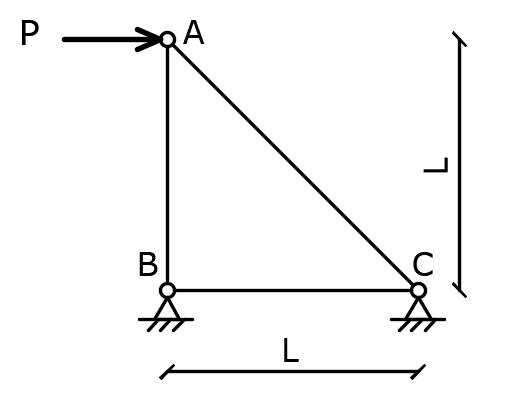
\includegraphics[width=0.45\linewidth]{UT2ej1}
\end{center}

Considerando que $P=50$ kN y $L=4.0$ m, se pide:

\parte Calcular las reacciones, los esfuerzos en todas las barras y el desplazamiento del nodo A mediante el Método de los Desplazamientos y el Método de las Fuerzas.

\parte Verificar lo hallado en la parte anterior mediante el empleo de alguna herramienta computacional.




\ejercicio

En la estructura reticulada mostrada en la figura cada barra está formada por 2 perfiles PNC10 de acero ($E=210$ GPa).

\begin{center}
	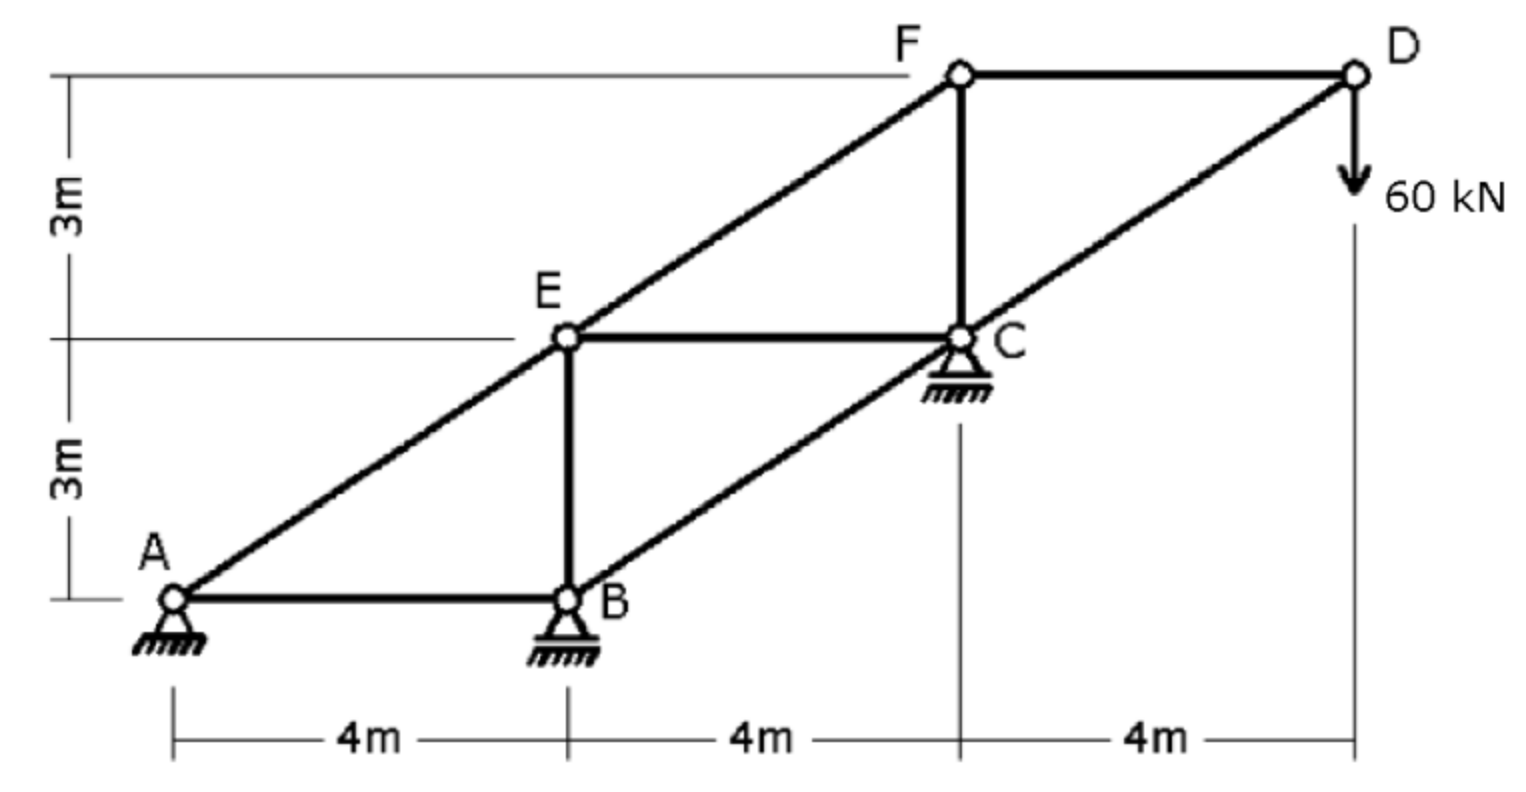
\includegraphics[width=0.8\linewidth]{UT2ej2}
\end{center}

Se pide:
%
\parte Calcular las reacciones, los esfuerzos en todas las barras y el desplazamiento del nodo D mediante el método de las fuerzas.
%
\parte Verificar lo hallado en la parte a) mediante el empleo de alguna herramienta computacional.




\ejercicio

En la estructura reticulada mostrada en la figura todas las barras tienen la misma sección y están formadas por el mismo material. %

\begin{center}
	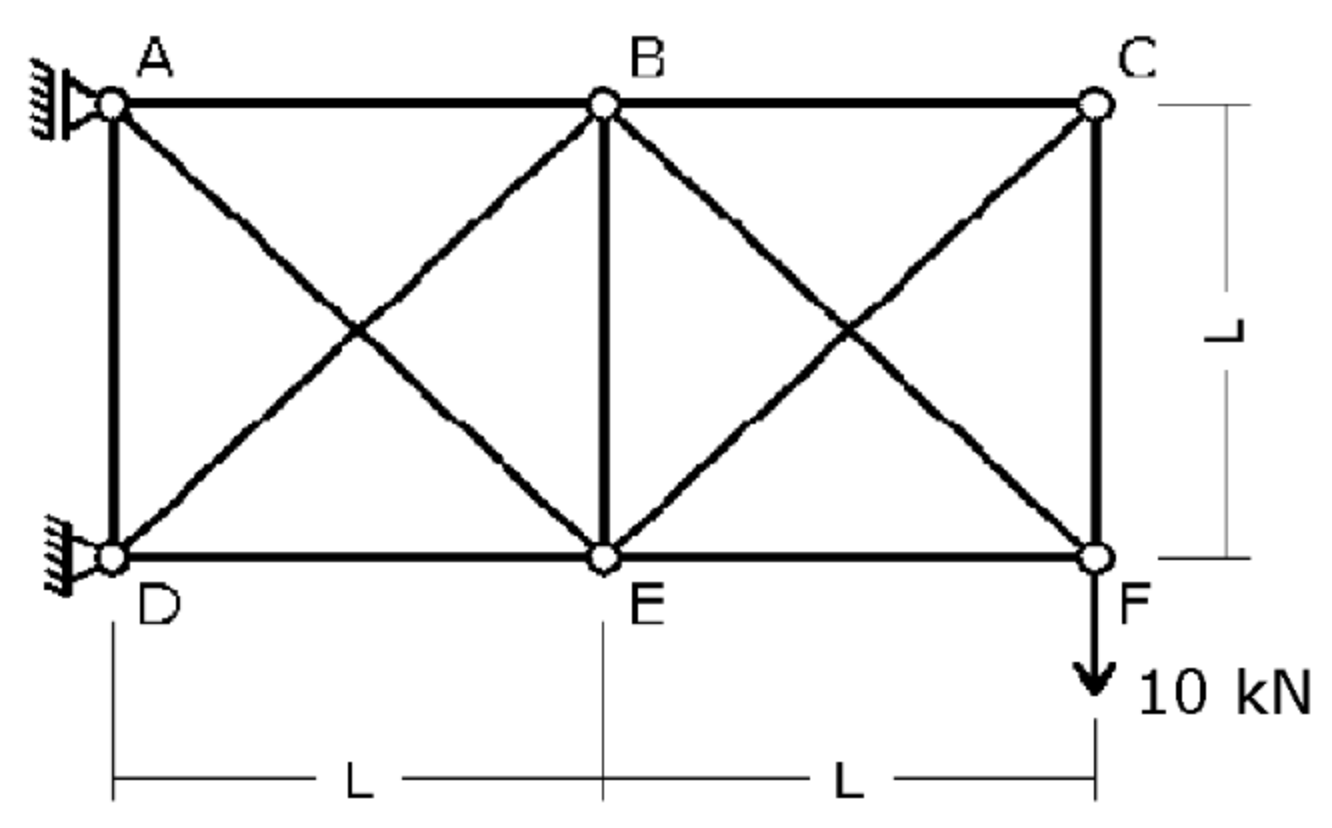
\includegraphics[width=0.6\linewidth]{UT2ej3}
\end{center}

Aplicando el Método de las Fuerzas, se pide:

\parte Calcular las reacciones y los esfuerzos en todas las barras.
%
\parte Si $L=1$ m, el área de cada barra $\Omega=4$ cm$^2$ y $E=210$ GPa, calcular el desplazamiento del nodo F.
%
\parte Verificar lo hallado en la parte a) y b) mediante alguna herramienta computacional.


\ejercicio

En la estructura reticulada mostrada en la figura, todas las barras tienen la misma sección y el mismo material.

\begin{center}
	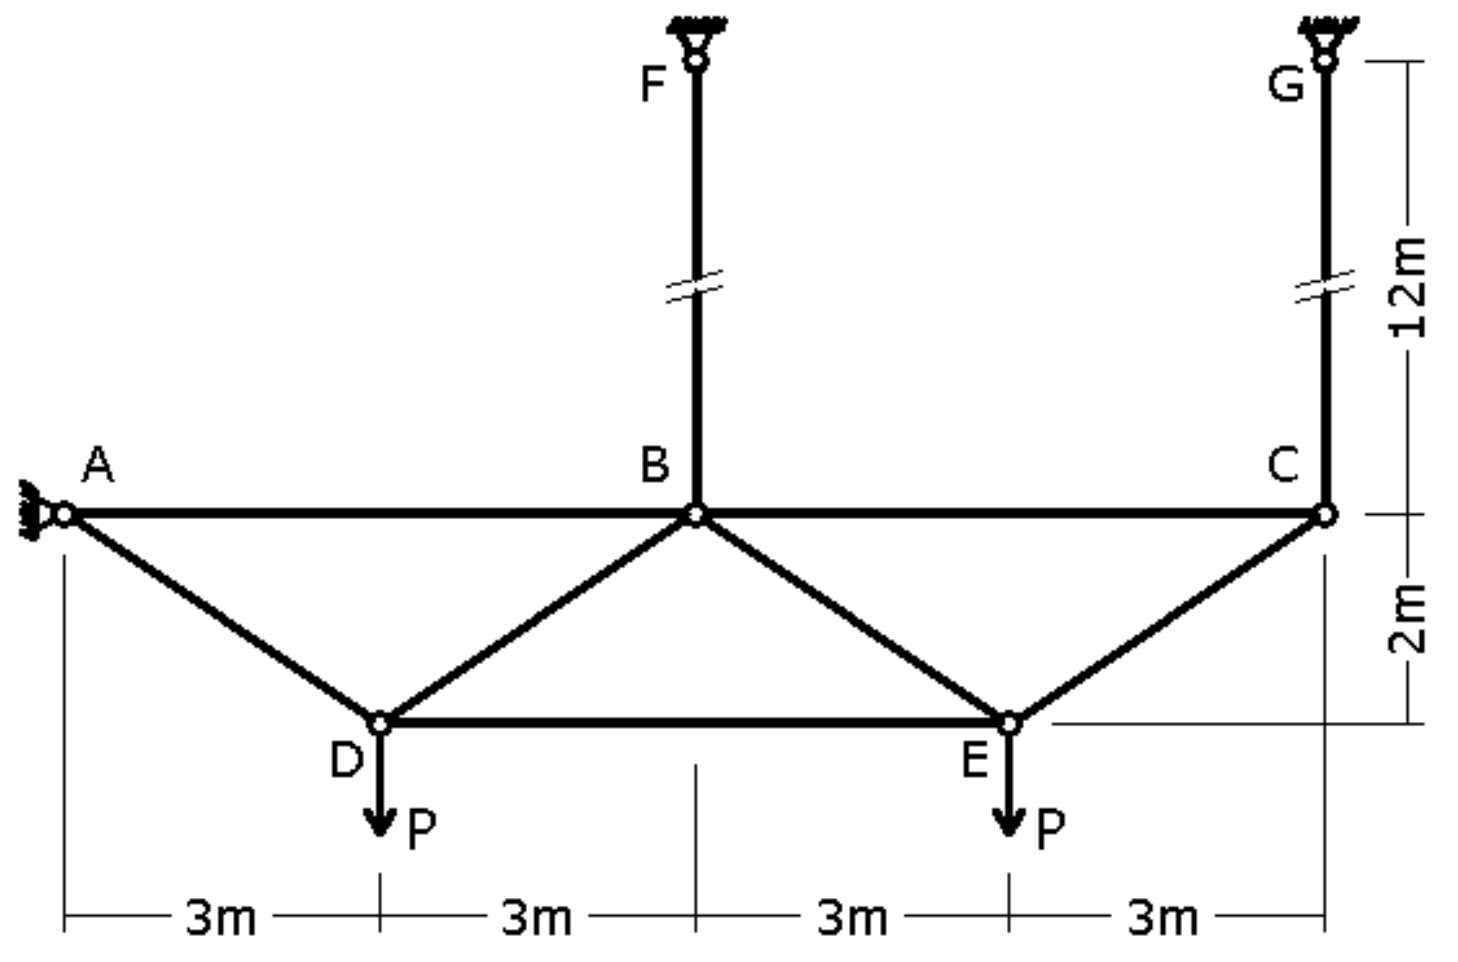
\includegraphics[width=0.75\linewidth]{UT2ej4}
\end{center}

Considerando  $P=10$ kN, $E=210$ GPa y $\Omega=1$ cm$^2$, se pide:
%
\parte Mediante el método de las fuerzas calcular las reacciones, los esfuerzos en todas las barras y el desplazamiento vertical de los nodos B y C. 
%
\parte Verificar lo hallado en la parte a) mediante alguna herramienta computacional.


\ejercicio
Sea el reticulado y las cargas que se muestran en la figura, donde todos los triángulos son equiláteros y las barras tienen todas mismo módulo de elasticidad y área.

\begin{center}
	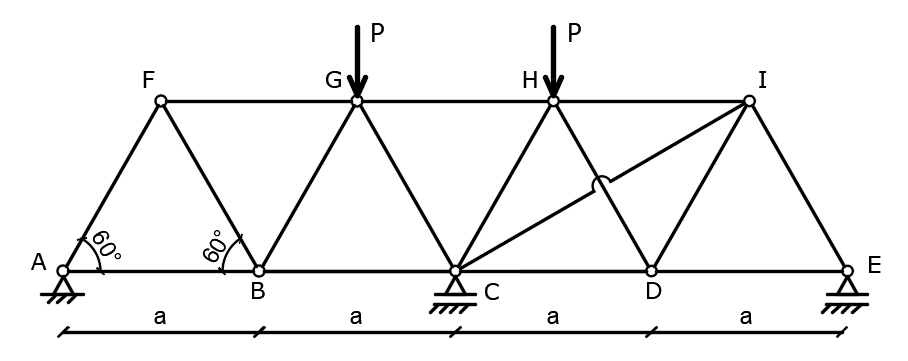
\includegraphics[width=0.95\linewidth]{UT2ej5}
\end{center}

Se pide:

\parte Calcular la solicitación de cada barra utilizando el método de las fuerzas.
\parte Dimensionar la estructura con perfiles PNI, suponiendo que todas las barras son iguales, para $P=300$ kN, $a=3$ m y $\sigma_{adm}=140$ MPa.


% codigoFuenteLibroR2
% Copyright (C) 2020  J.M. Perez Zerpa, et. al.
%
% This program is free software: you can redistribute it and/or modify
% it under the terms of the GNU General Public License as published by
% the Free Software Foundation version 3 of the License.
%
% This program is distributed in the hope that it will be useful,
% but WITHOUT ANY WARRANTY; without even the implied warranty of
% MERCHANTABILITY or FITNESS FOR A PARTICULAR PURPOSE. See the
% GNU General Public License for more details.
%
% You should have received a copy of the GNU General Public License
% along with this program.  If not, see <http://www.gnu.org/licenses/>.

\chapter[Método de Desplazamientos en pórticos]{Método de Desplazamientos en pórticos}

% intro e hipotesis
En esta Unidad Temática se presentan métodos de análisis de estructuras planas de barras en base a desplazamientos como incógnita principal. %
%
El enfoque adoptado para presentar el tema es similar al utilizado en \citep{Pilkey2002,Wunderlich2002}, utilizando los principios energéticos ya vistos en la Unidad Temática 2 de forma similar a como es realizado en \citep{Reddy2002b}.
% ----------------------------




\section{Teoría de vigas sometidas a flexión compuesta} \label{sec:teoviga}

\subsection{Hipótesis y definiciones fundamentales}

Para el análisis de pórticos es necesario abordar el estudio de vigas sometidas a cargas transversales y axiales, esto será llamado \textit{flexión compuesta}. %
%
Para esto, un posible camino es agregar el efecto de la directa a las ecuaciones de la teoría de vigas a flexión pura, presentadas en la sección \ref{sec:teovigastimo}. %
%
Sin embargo se optará por otro camino orientado a deducir las ecuaciones a partir de algunas hipótesis de la teoría de vigas integradas con la Teoría de la Elasticidad. %
%
Este enfoque es utilizado en literatura de referencia \citep{Wunderlich2002,Onate2013} y permite llegar a los mismos resultados.

\subsubsection{Hipótesis}
Sea el campo de desplazamientos de los puntos de la viga, dados por el vector formado por las funciones: $u(x,y,z)$, $v(x,y,z)$ y $w(x,y,z)$, representando desplazamientos en $x$, $y$ y $z$ respectivamente. %
%
Asumiendo que la flexión se produce en el plano $x-y$, se consideran las siguientes hipótesis:
%
\begin{enumerate}
	\item Los desplazamientos transversales (flecha) de todos los puntos en una sección transversal (ubicada en la coordenada $x$)  son pequeños e iguales al desplazamiento del eje de la viga.
	$$
	v(x,y,z) =  v(x).
	$$
	\item Las secciones transversales permanecen planas y perpendiculares al eje deformado durante la deformación y los giros $\theta$ son pequeños. %
	%
	Los desplazamientos axiales por tanto están dados por:
	\begin{equation} \label{eqn:despaxi}
	u(x,y,z) = u_G(x) - y \theta(x),
	\end{equation}
	donde $\theta$ es el ángulo que forma el vector tangente de la curva de la deformada del eje con la horizontal y $u_G(x)$ es la función del desplazamiento axial del baricentro de la sección ubicada en $x$. 
	%
	\item Todos los desplazamientos perpendiculares al plano de deformación de la viga son nulos
$$
w(x,y,z) = 0
$$
	%
	\item Se asume que no existen esfuerzos aplicados perpendiculares al plano de deformación de la viga
	\item Se desprecia la energía de deformación por cortante es decir, la distorsión angular.
\end{enumerate}

Respecto a la hipótesis de desplazamientos perpendiculares al plano, esta hipótesis representa una simplificación del comportamiento real de la estructura y el efecto de Poisson, sin embargo simplifica la aplicación de la ecuación constitutiva y el cálculo del tensor de deformaciones y permite llegar a las ecuaciones de la teoría de vigas de forma directa.

Respecto a la no consideración de energía de deformación por cortante, se recomienda al estudiante interesado libros como \citep{Onate2013} donde se describen los elementos de viga de Timoshenko o  artículos recientes en los que se muestra la utilidad de este tipo de enfoques para simular el comportamiento real de estructuras \citep{Bui2014}. %
%
En este curso no se considerará deformación por cortante, hipótesis que puede ser razonable para vigas cuya relación entre largo y altura de sección transversal sea superior a 10: $L/h > 10$ (este número es adoptado como criterio para este curso, otros estudios numérico/experimentales pueden sugerir otros valores).

\subsubsection{Tensor de deformaciones}

Se comienza calculando las componentes del tensor de deformaciones aplicando la relación desplazamientos-deformación al campo de desplazamientos considerado (ver Ecuación~\eqref{eqn:despaxi}). %
%
La tensión axial  $\varepsilon_x$ está dada por:
%
\begin{equation}\label{eqn:expdef}
\varepsilon_x(x,y) =  \varepsilon_G (x) -y \frac{\partial \theta}{\partial x}(x).
\end{equation}
%
donde $\varepsilon_G$ es la deformación axial del eje de la viga, y está dada por
%
\begin{equation}
\varepsilon_G(x) =  \frac{\partial u_G}{\partial x} (x) .
\end{equation}


La distorsión angular $\gamma_{xy}$ está dada por:
\begin{equation}
  \gamma_{xy}(x,y) = -\theta(x) + \frac{\partial v}{\partial x} (x).
\end{equation}
%
La no dependencia de $\gamma_{xy}$ respecto a $y$ implica que la cara permanece plana. %
%
Al imponer que la distorsión angular (asociada a la deformación por cortante) sea nula, se aporta la condición:
\begin{equation}
\boxed{
\theta = \frac{\partial v}{\partial x},
}
\end{equation}
lo que es equivalente a que la normal a la sección transversal deformada coincida con la tangente a la curva deformada.

Finalmente la expresión de la deformación axial está dada por:
%
\begin{equation}\label{eqn:epsdef}
\boxed{
\varepsilon_x(x,y) =  \varepsilon_G (x) -y \frac{\partial^2 v}{\partial x^2}(x).
}
\end{equation}
lo que representa una extensión de la expresión obtenida en la Ecuación~\eqref{eqn:epstimo} para el caso de deformación axial.

\cajaactividad{
Demostrar que, considerando las hipótesis de desplazamiento mencionadas, la única componente del tensor de deformaciones no nula, es $\varepsilon_{xx}$.
}



\subsubsection{Tensor de tensiones}

Se considera que el material es elástico lineal e isótropo. Se utiliza la correspondiente ecuación constitutiva y el tensor de deformaciones obtenido, teniendo la relación:
%
\begin{equation}
  \sigma_x = E \varep_x
\end{equation}

Esta componente de $\bfsig$ es la única que produce trabajo interno en la expresión de la energía interna de deformación dada por la Ecuación~\eqref{eqn:energbarra}.

\subsection{Solicitaciones y convenciones de signo}


\subsubsection{Solicitaciones internas}

Se definen las solicitaciones internas correspondientes a la tensión axial: directa y momento. %
%
Para la directa se tiene
%
\begin{equation}
N (x) = \int_{A(x)} \sigma_x (x,y) \, \dif A
\end{equation}
%
usando que la sección transversal es uniforme, la ecuación constitutiva y la expresión de la deformación axial se tiene:
%
\begin{equation}
N (x) = \int_{A(x)} \left( E \frac{\partial u_G}{\partial x} - E y \frac{\partial^2 v}{\partial x^2}   \right) \, \dif A.
\end{equation}
%
Usando que el vector $\bfe_x$ pasa por el punto $G$, baricentro de la sección transversal, se tiene
%
\begin{equation}\label{eqn:direc}
\boxed{
N (x) =  E A  \varepsilon_G(x).
}
\end{equation}
%
Se puede destacar que la convención de signo de directa positiva a tracción es coherente con el resultado obtenido ya que en dicho caso $\varepsilon_G >0$.

Para el cálculo del momento según el eje $\bfe_z$ se considera la suma (integral) del momento de diferenciales de área por su brazo respectivo:
%
\begin{equation}
M_z (x) = \int_{A(x)} \left( y \bfe_y \,  \wedge \, \sigma_x (x,y) \bfe_x \right) \cdot \bfe_z \dif A.
\end{equation}
%
Sustituyendo las expresiones de las tensiones y la deformación dada por la Ecuación~\eqref{eqn:expdef} se obtiene:
%
\begin{equation}
M_z (x) = \int_{A(x)} y E \varep_{G} \left( \bfe_y \,  \wedge \, \bfe_x \right) \cdot \bfe_z \dif A + \int_{A(x)} -y^2 \frac{\partial^2 v}{\partial x^2} (x)  \left( \bfe_y \,  \wedge \, \bfe_x \right) \cdot \bfe_z \dif A.
\end{equation}

Calculando el producto mixto y usando que el primer momento de inercia respecto al baricentro es nulo, se obtiene:
%
\begin{equation}
M_z (x) = E \int_{A(x)} y^2 \dif A \,  \frac{\partial^2 v}{\partial x^2} (x)
\end{equation}
%
usando que el material tiene sección transversal uniforme y definiendo el segundo momento de inercia respecto de $z$ como $I_z(x) = \int_{A} y^2 dA$ se obtiene:
%
\begin{equation}\label{eqn:momen}
\boxed{
M_z (x) = E I_z \frac{\partial^2 v}{\partial x^2}(x).
}
\end{equation}

Por simplicidad de notación, a continuación se omitirán los subíndices $z$ y el argumento $x$. %
%
Esta notación con subíndices volverá a ser utilizada al considerar problemas de flexión esviada.

La relación obtenida entre momento y curvatura es muy relevante para la caracterización del comportamiento de estructuras de vigas incluso cuando el comportamiento incluye fenómenos complejos como fisuración y otras no linealidades.


\subsubsection{Expresión de tensión axial en función de solicitaciones}


%
A partir de la expresiones de la directa, dada por la Ecuación~\eqref{eqn:direc}, y del momento, dado por la Ecuación~\eqref{eqn:momen}, se obtiene:
%
\begin{equation}
\varepsilon_G(x) = \frac{	N (x) }{E A}
\qquad
\frac{\partial^2 v}{\partial x^2}(x) = \frac{	M_z (x) }{E I_z} 
\end{equation}
%
Sustituyendo en la expresión de la deformación axial dada por la Ecuación~\eqref{eqn:epsdef} se obtiene:
%
\begin{equation}
\varepsilon_x(x,y) = \frac{	N (x) }{E A}  -y  \frac{ M_z (x) }{E I_z},
\end{equation}

y multiplicando por $E$ ambos miembros y usando la ecuación constitutiva se tiene
%
\begin{equation}
\boxed{
\sigma(x,y) = \frac{	N (x) }{A}
- y \frac{	M_z (x) }{I_z} 
}
\end{equation}


\subsubsection{Convenciones de signo}

Para el desarrollo de métodos de análisis de pórticos es útil y necesario definir una convención de signos diferente a la usada para las solicitaciones internas. %
%
En la \autoref{fig:conve} se muestran dos convenciones de signo a ser utilizadas en este documento y en todo el curso.
%
\begin{figure}[htb]
  \centering
  \def\svgwidth{0.8\textwidth}
  \input{figs/UT3/convenciones_signos_vigas.pdf_tex}
	\caption{Convenciones de signo para momentos nodales y cargas externas en coordenadas locales.}
	\label{fig:conve}
\end{figure}

Las \textbf{solicitaciones internas} definidas con la convención de signos usual para $\sigma$ (positivo tracción) corresponden a la convención de signos \textbf{1} de la figura. %
%
Esta convención corresponde a aquella en la cual momentos positivos representan una tracción de fibras inferiores.

Por otra parte, la convención \textbf{2} es útil para el desarrollo de métodos matriciales o computacionales, asociada a las \textbf{fuerzas externas} aplicadas.

\subsubsection{Ecuaciones de equilibrio}

Las ecuaciones para vigas sometidas a cargas transversales $q$ y axiales $b$ distribuidas por unidad de longitud están dadas por:
%
\begin{eqnarray}
\frac{dN}{dx}(x) & =& -b(x) \\
\frac{dV}{dx}(x) & =& q(x) \label{eqn:eqcortante}\\
\frac{\partial M}{\partial x}(x) & =& V(x)
\end{eqnarray}
%

La deducción de estas ecuaciones a partir del equilibrio de un segmento diferencial fue realizado en cursos anteriores. %
Por otra parte, este desarrollo también puede ser realizado a partir del teorema de trabajo virtual, de forma similar a como es hecho en la sección 5.4.5 de \citep{Hughes1987a}.


\subsection{Relaciones fuerzas-desplazamientos para vigas a flexión}\label{sec:mdvig}

Se considera una viga de largo $L$, formada por un material de módulo de Young $E$ y con sección transversal uniforme de inercia $I$ sometida a fuerzas aplicadas en los extremos de \textbf{cortante y momento} de acuerdo a la convención 2 de la \autoref{fig:conve}. %
%
Se asume que no hay cargas aplicadas en el tramo intermedio de la viga, ni distribuidas ni puntuales. %
%

Se considera que no hay deformación axial o esta es despreciable ($\varep_{G}\approx 0$). %
%
También se omitirá el sub-índice $z$ en $M_z$ y $\theta_z$. 

\subsubsection{Ecuación de la elástica}

A partir de las ecuaciones de equilibrio y la ecuación de la elástica se obtiene que la flecha es una función de tercer grado, por lo que se considera la siguiente expresión polinómica general:
%
\begin{equation}\label{eqn:ecw}
v(x) = a_3 x^3 + a_2 x^2 + a_1 x + a_0, \qquad \forall x \in [0,L].
\end{equation}

En lugar de trabajar con los parámetros $a_i$ se desea representar la función $v$ en función de los valores nodales de flecha y giro, es decir, $v_1$,  $\theta_1$, $v_2$ y $\theta_2$. %
%
Para esto, se plantean las siguientes relaciones entre la flecha $v$ evaluada en ciertos puntos en particular y los desplazamientos nodales:
%
\begin{equation}
v_1 = v(0), \qquad
\theta_1 = \frac{d v}{d x} (0), \qquad
v_2 = v(L), \qquad
\theta_2 = \frac{d v}{d x}(L).
\end{equation}

Resolviendo el sistema de ecuaciones lineales se obtiene:
%
\begin{eqnarray}
a_3 &=& \frac{1}{L^3} \left( \theta_{1} L + \theta_{2} L + 2 v_{1} - 2 v_{2} \right) \nonumber\\
a_2 &=&	\frac{1}{L^2} \left( - 2 \theta_{1} L - \theta_{2}  L - 	3 v_{1} + 3 v_{2}  \right) \nonumber\\
a_1 &=&	\theta_{1} \nonumber\\
a_0 &=&	v_{1}, \nonumber
\end{eqnarray}
%
y sustituyendo en la Ecuación~\eqref{eqn:ecw} se obtiene la expresión:
%
\begin{equation} \label{eqn:elastica}
v(x) =  \varphi_{v_1}(x) v_1 + \varphi_{\theta_1}(x) \theta_1
+ \varphi_{v_2}(x) v_2 + \varphi_{\theta_2}(x) \theta_2,
\end{equation}
%
donde las funciones $\varphi$ son funciones de interpolación dadas por:
%
\begin{eqnarray}
\varphi_{v_1} (x) &=& \left(1 - \frac{3 x^{2}}{L^{2}} + \frac{2 x^{3}}{L^{3}}\right) \\
\varphi_{\theta_1} (x) &=&	\left(x - \frac{2 x^{2}}{L} + \frac{x^{3}}{L^{2}}\right) \\
\varphi_{v_2} (x) &=&	\left(\frac{3 x^{2}}{L^{2}} - \frac{2 x^{3}}{L^{3}}\right) \\
\varphi_{\theta_2} (x) &=& \left(- \frac{x^{2}}{L} + \frac{x^{3}}{L^{2}}\right) .
\end{eqnarray}

En la \autoref{fig:phis} se muestran los gráficos de las funciones de interpolación, los cuales corresponden a las funciones de las elásticas para desplazamientos o giros unitarios de cada grado de libertad correspondiente. %
%

%
\begin{figure}[htb]
	\centering
	\subfloat[Funciones de interpolación $\varphi_{v_1}$ y $\varphi_{v_2}$.]{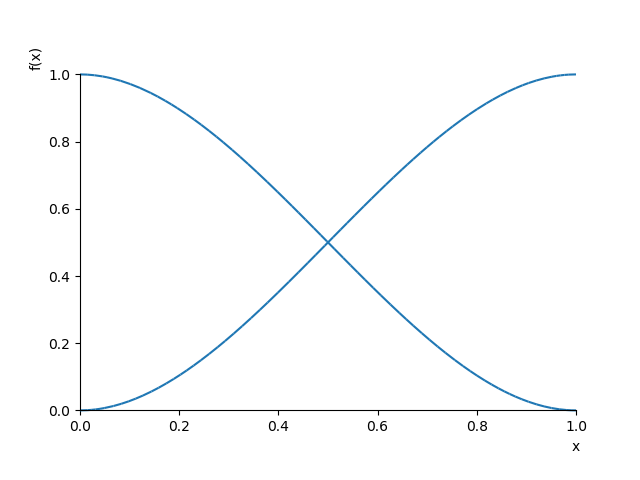
\includegraphics[width=0.47\textwidth]{phisv}\label{fig:phiv}}
	\subfloat[Funciones de interpolación $\varphi_{\theta_1}$ y $\varphi_{\theta_2}$.]{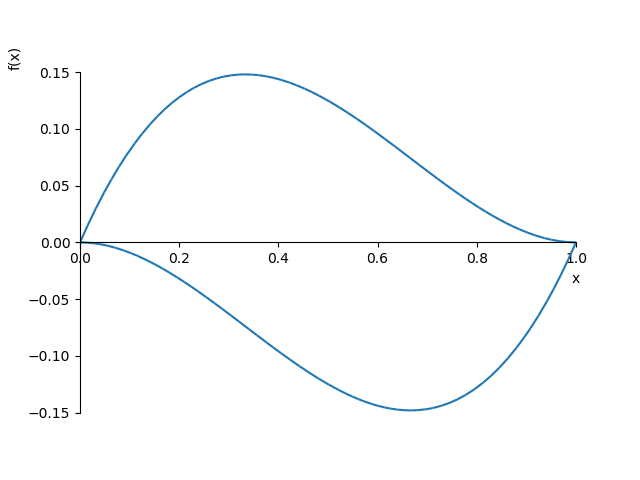
\includegraphics[width=0.47\textwidth]{phist}\label{fig:phit}}
	\caption{Gráfico de funciones de interpolación para $L=1$.}
	\label{fig:phis}
\end{figure}




\subsubsection{Mínima energía potencial y teorema de Castigliano}


Se tiene entonces definidas las funciones de interpolación $\phi$ definidas al inicio de la UT2, correspondientes al caso de vigas a flexión pura.
%
Se tiene también las expresiones de la deformación axial y la ecuación constitutiva por lo que se está en condiciones de aplicar el principio de mínima energía potencial. Aplicando el principio se obtendrán las relaciones entre fuerzas y desplazamientos para las cuales se cumplen con ecuaciones de compatibilidad de desplazamientos y equilibrio con fuerzas externas.

Dado que se desprecia la energía de deformación por cortante (asociada al producto $\tau_{xy} \gamma_{xy}$), la energía potencial de deformación de la viga está dada por:
%
\begin{equation}
\Pi_{int} = \frac{1}{2} \int_\Omega \bfsig : \bfvarep  \dif V  = \frac{1}{2} \int_\Omega \sigma_x \varepsilon_x  \dif V. 
\end{equation}

Sustituyendo las ecuaciones \eqref{eqn:eccons} y \eqref{eqn:expdef} y usando que se desprecia la deformación axial $\varep_G$ se tiene:
%
\begin{equation}\label{eqn:ut3piviga}
\Pi_{int} = \frac{1}{2} \int_0^L \int_{A(x)} E y^2 \left( \frac{\partial^2 v}{\partial x^2}\right)^2  \dif A \dif x 
=  E I  \frac{1}{2} \int_0^L \left( \frac{\partial^2 v}{\partial x^2}\right)^2 \dif x .
\end{equation}

%
Se destaca que fue despreciada la energía de deformación axial por directas (en caso de que fueran aplicadas) es decir que el término $EA\varepsilon_G^2$ se consideró mucho menor que $EI \kappa^2$.

Usando la Ecuación~\eqref{eqn:elastica} se obtiene la energía de deformación en función de los desplazamientos y giros nodales $\Pi_{int}(v_1,\theta_1,v_2,\theta_2)$.

Para este desarrollo se considera la convención de signos 2 tanto para fuerzas y momentos como para desplazamientos. %
%
De esta forma la energía potencial de las fuerzas externas está dada por:
\begin{equation}
\Pi_{ext}(v_1,\theta_1,v_2,\theta_2) = - F_{y,1} v_1 - M_1 \theta_1  - F_{y,2} v_2 - M_2 \theta_2,
\end{equation}
%
y por lo tanto, la energía potencial total está dada por:
\begin{equation}
\Pi(v_1,\theta_1,v_2,\theta_2) =  \Pi_{int}(v_1,\theta_1,v_2,\theta_2)  - F_{y,1} v_1 - M_1 \theta_1 - F_{y,2} v_2 - M_2 \theta_2,
\end{equation}

Las condiciones de mínima energía potencial total pueden por lo tanto ser escritas como:
%
\begin{eqnarray}
\frac{\partial \Pi_{int}}{\partial v_1}(v_1,\theta_1,v_2,\theta_2) &=&  F_{y,1} \\
\frac{\partial \Pi_{int}}{\partial \theta_1}(v_1,\theta_1,v_2,\theta_2) &=&  M_1 \label{eqn:ut3castm1} \\
\frac{\partial \Pi_{int}}{\partial v_2}(v_1,\theta_1,v_2,\theta_2) &=&  F_{y,2} \\
\frac{\partial \Pi_{int}}{\partial \theta_2}(v_1,\theta_1,v_2,\theta_2) &=&  M_2
\end{eqnarray}


A modo de ejemplo se presenta el desarrollo para la condición del momento del nodo izquierdo, es decir, la Ecuación~\eqref{eqn:ut3castm1}. %
%
Usando la interpolación de la flecha en la Ecuación~\eqref{eqn:ut3piviga} y calculando la derivada, se tiene:
%
\begin{equation}
\frac{\partial \Pi_{int}}{\partial \theta_1} = \frac{1}{2} EI \int_0^{L} 2 \left( \frac{\partial^2 v}{\partial x^2} (v_1,\theta_1,v_2,\theta_2) \varphi_{\theta_1}'' \right) \dif x
\end{equation}
%
para evaluar la derivada de $v$ se utilizan las expresiones de las derivadas de las funciones de interpolación dadas por:
%
\begin{eqnarray}
	\varphi_{v_1}'' (x) = \left(- \frac{6}{L^{2}} + \frac{12 x}{L^{3}}\right) \qquad %
	\varphi_{\theta_1}'' (x) =	\left( - \frac{4}{L} + \frac{6 x }{L^{2}}\right) \\
	\varphi_{v_2}'' (x) =	\left(\frac{6}{L^{2}} - \frac{12 x}{L^{3}}\right) \qquad %
	\varphi_{\theta_2}'' (x) = \left(- \frac{2}{L} + \frac{6 x}{L^{2}}\right) .
\end{eqnarray}
%
sustituyendo $v$ por la expresión dada por las funciones de interpolación se obtiene:
%
\begin{equation}
\frac{\partial \Pi_{int}}{\partial \theta_1} = K_{v_1,\theta_1} v_1 + K_{\theta_1,\theta_1} \theta_1 + K_{v_2,\theta_1} v_2  + K_{\theta_2,\theta_1} \theta_2
\end{equation}
%
donde los coeficientes $K$ están dados por las integrales:
%
\begin{eqnarray}
K_{v_1,\theta_1} = EI \int_0^L \varphi_{v_1}'' \varphi_{\theta_1}'' \dif x \qquad
%
K_{\theta_1,\theta_1} = EI \int_0^L \varphi_{\theta_1}'' \varphi_{\theta_1}'' \dif x \\
%
K_{v_2,\theta_1} = EI \int_0^L \varphi_{v_2}'' \varphi_{\theta_1}'' \dif x \qquad 
%
K_{\theta_2,\theta_1} = EI\int_0^L \varphi_{\theta_2}'' \varphi_{\theta_1}'' \dif x 
\end{eqnarray}
%
Calculando las integrales se tiene:
%
\begin{eqnarray}
K_{v_1,\theta_1} &=& EI \left(   \frac{24}{L^2} -  \frac{84}{2} \frac{1}{L^2} + \frac{72}{3} \frac{1}{L^2} \right) = EI \frac{6}{L^2} \\
%
K_{\theta_1,\theta_1} &=& EI \left(   \frac{16}{L^2} -  \frac{48}{2}\frac{1}{L^2} +\frac{36}{3} \frac{1}{L^2}  \right) L = EI \frac{4}{L}\\
%
K_{v_2,\theta_1} &=& EI \left(  - \frac{24}{L^2} + \frac{84}{2} \frac{1}{L^2} - \frac{72}{3} \frac{1}{L^2} \right) = -EI \frac{6}{L^2} \\
%
K_{\theta_2,\theta_1} &=& EI \left(   \frac{8}{L^2} -  \frac{36}{2} \frac{1}{L^2} + \frac{36}{3} \frac{1}{L^2}  \right)L = EI \frac{2}{L}
\end{eqnarray}

Se obtiene por lo tanto que la ecuación de Castigliano para el giro del primer nodo, dada por la Ecuación~\eqref{eqn:ut3castm1}, puede ser escrita como:
%
\begin{equation}
EI \frac{6}{L^2} v_1 +  EI \frac{4}{L} \theta_1 - EI \frac{6}{L^2} v_2 +    EI \frac{2}{L} \theta_2 = M_1.
\end{equation}


Repitiendo el procedimiento para las otras condiciones de Castigliano se llega a:
%
\begin{eqnarray}
EI \left( \dfrac{12}{L^{3}} v_1 + \dfrac{6}{L^{2}} \theta_1 - \dfrac{12}{L^{3}} v_2 + \dfrac{6}{L^{2}} \theta_2 \right)  &=& F_{y,1} \\
EI \left( \frac{6}{L^2} v_1 +  \frac{4}{L} \theta_1 - \frac{6}{L^2} v_2   + \frac{2}{L} \theta_2 \right) &=& M_1 \\
EI \left( -\dfrac{12}{L^{3}} v_1 - \dfrac{6}{L^{2}} \theta_1 +\dfrac{12}{L^{3}} v_2 - \dfrac{6}{L^{2}} \theta_2 \right) &=& F_{y,2} \\
EI \left( \dfrac{6}{L^{2}} v_1 + \dfrac{2}{L} \theta_1 - \dfrac{6}{L^{2}} v_2 + \dfrac{4}{L}  \theta_2 \right) &=& M_2,
\end{eqnarray}
%

Estas ecuaciones representan un sistema de ecuaciones cuyas incógnitas son los desplazamientos y giros y el dato o término independiente son las fuerzas. %
%
Estas relaciones pueden ser escritas en forma matricial como
\begin{equation}
\bfK \bfu = \bff	
\end{equation}
%
donde
\begin{equation}
\bfK =  EI \left[
\begin{matrix}
\dfrac{12}{L^{3}}  & \dfrac{6}{L^{2}} & - \dfrac{12}{L^{3}} & \dfrac{6}{L^{2}} \\[3mm]
\dfrac{6}{L^2}  & \dfrac{4}{L} & - \dfrac{6}{L^2} & \dfrac{2}{L}  \\[3mm]
-\dfrac{12}{L^{3}} & - \dfrac{6}{L^{2}} & \dfrac{12}{L^{3}} & - \dfrac{6}{L^{2}} \\[3mm]
\dfrac{6}{L^{2}} & \dfrac{2}{L} & - \dfrac{6}{L^{2}} & \dfrac{4}{L} 
\end{matrix}
\right]
\quad \text{y}\quad
\bff =  \left[
\begin{matrix}
F_{y,1} \\[3mm]
M_{1} \\[3mm]
F_{y,2} \\[3mm]
M_{2} \\
\end{matrix}
\right]
\end{equation}



%
Es importante destacar qué condiciones de contorno (en los desplazamientos) deben ser aplicadas para poder obtener una solución única, es decir, eliminar los posibles movimientos de cuerpo rígido que tenga la viga.



\cajaactividad{
Calcular la flecha máxima de una viga de largo $\ell$, biempotrada, con rigidez flexional uniforme $E I$ y una carga puntual $P$ aplicada en la mitad de su longitud, usando el método de los desplazamientos en su forma matricial, utilizando dos elementos.
}


%\subsection{Ejemplo}

%\subsection{Principio de trabajos virtuales}

%El principio de trabajos virtuales establece que la elástica de equilibrio $w(x)$ será aquella que cumpla que
%%
%\begin{equation}
%EI \int_{0}^{L} \frac{d^2 w}{d x^2} \, \frac{d^2 \tilde{w} }{d x^2} \, \dif x = V_1 \tilde{w}_1 +  M_1 \tilde{\theta}_1 + V_2 \tilde{w}_2 + M_2 \tilde{\theta}_2
%\end{equation}
%



\section{Métodos de analíticos para pórticos}


\subsection{Ecuaciones para métodos analíticos}

Los métodos analíticos de resolución se basan en el planteo de las ecuaciones para cada elemento de la estructura independientemente e imponer condiciones de equilibrio en los nodos de unión correspondientes. %
%
Para aplicar estos métodos es conveniente definir variables auxiliares como $\psi$, dada por la expresión:
%
\begin{equation}
  \psi = \frac{v_2 - v_1}{L}.
\end{equation}
%

$\psi$ puede ser interpretado geométricamente como el giro antihorario (en pequeños giros) de la recta que une los dos nodos (cuerda). Se puede ver un diagrama en la \autoref{fig:psi}.

\begin{figure}[htb]
	\centering
	\def\svgwidth{0.65\textwidth}
	\input{figs/UT3/diagramaPsi.pdf_tex}
	\caption{Diagrama para interpretación geométrica de $\psi$.}
	\label{fig:psi}
\end{figure}


Las ecuaciones de Castigliano asociadas a los momentos pasan a ser: %
%
\begin{equation}\label{eqn:eqvig}
\left\{
\begin{array}{rl}
\displaystyle
\frac{2 EI}{L} \left( 2 \theta_1  + \theta_2 - 3 \psi   \right) =& M_1 \\[3mm]
\displaystyle
\frac{2 EI}{L} \left( \theta_1 + 2  \theta_2 - 3 \psi  \right) =& M_2
\end{array}
\right.
\end{equation}

Por otra parte a partir de combinaciones lineales de las ecuaciones de momento y cortante se obtiene las relaciones:
%
\begin{equation}
\left\{
\begin{array}{rl}
\displaystyle
F_{y,1} & \displaystyle
 = \frac{M_1 + M_2}{L} \\[5mm]
\displaystyle
F_{y,2} & \displaystyle
 = -\frac{M_1 + M_2}{L} 
\end{array}
\right.
\end{equation}

Estas ecuaciones son planteadas para cada elemento de barra y los momentos que actúan sobre cada nodo son considerados en ecuaciones de equilibrio nodal, obteniendo así el número de ecuaciones necesarias para obtener todos los desplazamientos y giros.




\subsection{Cargas equivalentes}

En el caso en que la barra tenga cargas aplicadas entre los nodos se puede considerar fuerzas y momentos aplicados en los nodos con la misma energía potencial externa. %
%
Estas fuerzas nodales son llamadas cargas equivalentes. %
%
Este método permite obtener valores exactos de giros y flechas nodales, sin embargo, es necesario integrar las ecuaciones de equilibrio para obtener los diagramas de solicitaciones  y elástica en el tramo.

%La energía potencial de las cargas aplicadas estas cargas es:
%
%\begin{equation}
%V_{ext}^{tr} = -\int_{0}^{L} q(x) v(x) \dif x - P v(x_P)
%\end{equation}
%
%nuevamente se utiliza la expresión de la elástica de la Ecuación~\eqref{eqn:elastica}. 

A continuación se consideran dos casos importantes de cargas en el tramo, con un enfoque como el presentado en \citep{Onate2013} donde se puede encontrar un desarrollo más completo. %

\subsubsection{Carga distribuida}

En el caso de carga distribuida $q(x)$ (de acuerdo a la convención 2), se tiene que la energía potencial de las fuerzas $\Pi^{tr}_{ext}$ está dada por:
%
\begin{equation}
\Pi_{ext}^{tr} =
- \int_0^L q(x) v(x) \dif x.
\end{equation}
%
El objetivo es entonces encontrar las fuerzas nodales equivalentes que tengan la misma energía potencial. Para esto se sustituye la expresión de $v(x)$ dada por la Ecuación~\eqref{eqn:elastica}, obteniendo:
%
\begin{equation}
\Pi_{ext}^{tr} =
-F_{y,1}^{tr} v_1 - M_1^{tr} \theta_1 -F_{y,2}^{tr} v_2 -  M_2^{tr} \theta_2
\end{equation}
donde
\begin{eqnarray}
F_{y,1}^{tr} = \int_{0}^{L} q(x) \varphi_{v_1}(x) \dif x \qquad & \displaystyle M_1^{tr} = \int_{0}^{L}q(x) \varphi_{\theta_1}(x)  \dif x  \nonumber\\
F_{y,2}^{tr} = \int_{0}^{L}q(x) \varphi_{v_2}(x)  \dif x \qquad & \displaystyle M_2^{tr} = \int_{0}^{L} q(x)\varphi_{\theta_2}(x)  \dif x  \nonumber
\end{eqnarray}

En el caso particular de carga distribuida uniforme $q(x) = q$ se tiene:
%
\begin{eqnarray}
F_{y,1}^{tr} &=& \frac{q L}{2} \\
M_1^{tr} &=& \frac{q L^{2}}{12} \\
F_{y,2}^{tr} &=& \frac{q L}{2} \\
M_2^{tr} &=& - \frac{q L^{2}}{12}
\end{eqnarray}

\cajaconcepto{Empotramiento perfecto}{
Es importante ver que estas fuerzas nodales corresponden a los valores opuestos a las reacciones de una viga biempotrada, también llamadas momentos de \textit{empotramiento perfecto} $M^{emp}$ y sus respectivas fuerzas verticales o de cortante $F_y^{emp}$. %
%
Los cortantes y momentos de empotramiento perfecto son opuestos a sus correspondientes fuerzas de tramo, es decir: $F_y^{emp} = -F_y^{tr}$ y $M^{emp} = -M^{tr}$.
}

\subsubsection{Carga puntual}

Se considera ahora que la carga puntual $P$ es aplicada (según la convención 2) en el punto de coordenada $x= x_P$ con $x_P \in (0,L)$ y que $q(x)=0$.

La energía potencial de la fuerza en el tramo está dada por:
%
\begin{equation}
\Pi_{ext}^{tr} = - P v (x_P) =  -P \varphi_{v_1}(x_P) v_1 - P \varphi_{\theta_1}(x_P) \theta_1
- P \varphi_{v_2}(x_P) v_2 - P \varphi_{\theta_2}(x_P) \theta_2,
\end{equation}
%
por lo tanto las fuerzas nodales equivalentes a la carga puntual en $x_P$ son calculadas evaluando las funciones $\varphi$. %
%
Por ejemplo el momento nodal en 1 es
%
\begin{equation}
M_1^{tr} = P \varphi_{\theta_1} (x_P) = P  \left(x_P - \frac{2 x_P^{2}}{L} + \frac{x_P^{3}}{L^{2}}\right)
\end{equation}
%
expresión que, factorizando, puede ser reescrita como:
\begin{equation}
M_1^{tr} = P x_P (L-x_P)^2 \frac{1}{L^2}.
\end{equation}
Se verifica nuevamente que el momento equivalente es el opuesto del momento de empotramiento perfecto.

Para el otro momento se tiene
\begin{equation}
M_2^{tr} = -P x_P^2 (L-x_P) \frac{1}{L^2}.
\end{equation}

%
%\subsection{Ejemplo}
%
%%Para verificar los valores de las fuerzas nodales para la carga puntual consideramos un problema con solución conocida. %
%%
%En clase se resolverá el problema de una ménsula de módulo de Young $E$ inercia $I$ y largo $L$ con una carga aplicada $P$ en $x_P$ como se muestra en la figura.
%\begin{center}
%	\setlength{\unitlength}{0.5\textwidth}
%	\begin{picture}(1,0.33597629)%
%	\put(0,0){\includegraphics[width=\unitlength,page=1]{mensula_carga_puntual_tramo.pdf}}%
%	\put(0.24867277,0.06426678){\color[rgb]{0,0,0}\makebox(0,0)[lb]{\smash{$x_P$}}}%
%	\put(0.49097862,0.25976283){\color[rgb]{0,0,0}\makebox(0,0)[lb]{\smash{$P$}}}%
%	\put(0,0){\includegraphics[width=\unitlength,page=2]{mensula_carga_puntual_tramo.pdf}}%
%	\end{picture}%
%\end{center}

%Sabemos que los desplazamiento y giro del extremo derecho son
%$$
%w_2 = - \frac{Px_P^2}{6 EI} (3 L -x_P) \qquad \theta_2 = -\frac{P x_P^2}{2 EI}
%$$
%
%Resolvemos ahora aplicando el método. El sistema de ecuaciones es
%
%\begin{eqnarray}
%EI \frac{12}{L^3} w_2 - EI \frac{6}{L^2} \theta_2 & = & -P \left( \frac{3 x_P^2}{L^2} - \frac{2 x_P^3}{L^3} \right) \nonumber\\
%EI \frac{-6}{L^2} w_2 + EI \frac{4}{L} \theta_2 & = & -P \left( -\frac{ x_P^2}{L} + \frac{x_P^3}{L^2} \right) \nonumber
%\end{eqnarray}
%
%multiplicando la segunda ecuación por $2/L$ y sumando la primera se tiene
%
%\begin{equation}
%EI \left(  \frac{-6}{L^2} + \frac{8}{L^2} \right) \theta_2 = -P \left( 3 \frac{ 3x_P^2}{L^2} - \frac{2 x_P^2}{L^2} -  \frac{2 x_P^3}{L^3} + \frac{2 x_P^3}{L^3}  \right)
%\end{equation}
%
%simplificando y despejando se llega a 
%
%\begin{equation}
%\theta_2 = -\frac{P x_P^2}{2 EI}
%\end{equation}
%
%sustituyendo en la primer ecuación se tiene
%
%\begin{equation}
%EI \frac{-6}{L^2} w_2 + EI\frac{4}{L} \left(-\frac{P x_P^2}{2 EI}\right) = -P \left(  \frac{-x_P^2}{L}  + \frac{x_P^3}{L^2} \right)
%\end{equation}
%
%simplificando y despejando se llega a
%
%\begin{equation}
%w_2 = - \frac{Px_P^2}{6 EI} (3 L -x_P)
%\end{equation}
%
%

\subsubsection{Expresión de ecuaciones}

Las ecuaciones de relación fuerza-desplazamiento de la Ecuación~\eqref{eqn:eqvig} pasan a ser entonces:
\begin{equation}\label{eqn:ecmomtr}
\boxed{
\left\{
\begin{array}{rl}
\displaystyle
\frac{2 EI}{L} \left( 2 \theta_1  + \theta_2 - 3 \psi   \right) + M_1^{emp} =& M_1  \\[3mm]
\displaystyle
\frac{2 EI}{L} \left( \theta_1 + 2  \theta_2 - 3 \psi  \right) + M_2^{emp} =& M_2 
\end{array}
\right.
}
\end{equation}


Al considerar las fuerzas de tramo en las ecuaciones de fuerzas verticales y operar se tienen las siguientes expresiones:
%
\begin{equation}\label{eqn:eccortr}
\left\{
\begin{array}{rl}
\displaystyle
F_{y,1} + F_{y,1}^{tr} & \displaystyle
= \frac{M_1 + M_2}{L} + \frac{M_1^{tr} + M_2^{tr}}{L} \\[5mm]
\displaystyle
F_{y,2} + F_{y,2}^{tr} & \displaystyle
= -\frac{M_1 + M_2}{L} - \frac{M_1^{tr} + M_2^{tr}}{L}
\end{array}
\right.
\end{equation}
%

Agrupando se puede obtener que esto es equivalente a las ecuaciones:
%
\begin{equation}
\boxed{
\left\{
\begin{array}{rl}
\displaystyle
F_{y,1} & \displaystyle
= \frac{M_1 + M_2}{L} + F_{y,1}^{tr-iso} \\[5mm]
\displaystyle
F_{y,2}  & \displaystyle
= -\frac{M_1 + M_2}{L} + F_{y,2}^{tr-iso} 
\end{array}
\right.
}
\end{equation}
%
donde
%
\begin{eqnarray}
F_{y,1}^{tr-iso} = - F_{y,1}^{tr} + \frac{M_1^{tr} + M_2^{tr}}{L} \nonumber\\ 
F_{y,2}^{tr-iso} = -F_{y,2}^{tr}- \frac{M_1^{tr} + M_2^{tr}}{L} \nonumber
\end{eqnarray}
%
donde $F_{y,1}^{tr-iso}$ y $F_{y,2}^{tr-iso}$ son las cargas equivalentes correspondientes a las reacciones de una viga simplemente apoyada (cargas de tramo isostáticas). %
%
Esto se desarrollará con mayor detalle en el momento de aplicación en práctico.


\cajaactividad{
Repetir el cálculo de la flecha máxima de la viga bi-empotrada, mencionado anteriormente, utilizando cargas equivalentes para la carga puntual $P$.
}

\subsection{Expresiones para un extremo articulado}

En el caso de articulaciones en un extremo de la viga se puede obtener una expresión simplificada de la Ecuación~\eqref{eqn:eqvig}. %
%
Se considera una articulación en el nodo 2, entonces se puede imponer que $M_2=0$ obteniendo  
%
\begin{equation}
\frac{2 EI}{L} \left( \theta_1 + 2  \theta_2 - 3 \psi  \right) = 0 + M_2^{tr}
\end{equation}
%
por lo que despejando $\theta_{2}$ se tiene
%
\begin{equation} \label{eqn:artictheta2}
\theta_2 = -\frac{\theta_1}{2} + \frac{3}{2} \psi + \frac{M_2^{tr} L }{4 EI}.
\end{equation}

Sustituyendo en la ecuación del momento $M_1$ se tiene
%
\begin{equation}
\frac{2 EI}{L} \left( 2 \theta_1 + \left( -\frac{\theta_1}{2} + \frac{3}{2} \psi + \frac{M_2^{tr} L }{4 EI} \right) - 3 \psi  \right) = M_1 + M_1^{tr}.
\end{equation}
%
Finalmente operando se obtiene:
%
\begin{equation} \label{eqn:ecmomart}
\frac{3 EI}{L} \left( \theta_1 - \psi  \right) = M_1 + M_1^{tr} - \frac{ M_2^{tr}}{2}
\end{equation}
%
que puede ser escrita como
%
\begin{equation}
\boxed{
\frac{3 EI}{L} \left( \theta_1 - \psi  \right) + M_1^{emp'} = M_1
}
\end{equation}
%
donde $M_1^{emp'} = - M_1^{tr} + \frac{ M_2^{tr}}{2} $ es el momento de empotramiento perfecto (reacción) de una viga empotrada-articulada. %
%
Fácilmente obtenible utilizando tablas.


De forma análoga, si se tiene una articulación en el nodo 1, se impone $M_1=0$ y se tiene
por lo que despejando $\theta_{2}$ se tiene
%
\begin{equation} \label{eqn:artictheta1}
\theta_1 = -\frac{\theta_2}{2} + \frac{3}{2} \psi + \frac{M_1^{tr} L }{4 EI}.
\end{equation}

obteniendo la expresión de momento:%
\begin{equation}
\boxed{
	\frac{3 EI}{L} \left( \theta_2 - \psi  \right) + M_2^{emp'} = M_2
}
\end{equation}


%\subsection{Viga bi-articulada}
%
%%
%\begin{equation}
%\theta_1 = \frac{L}{3 EI} ( M_1^{tr} - \frac{ M_2^{tr}}{2}) + \psi  
%\end{equation}
%
%sustituyendo en \eqref{eqn:artictheta2} se tiene
%
%\begin{equation}
%\theta_2 = -\frac{L}{6 EI} ( M_1^{tr} - \frac{ M_2^{tr}}{2}) - \psi0.5   + \frac{3}{2} \psi + \frac{M_2^{tr} L }{4 EI}.
%\end{equation}
%

\subsection{Apoyos elásticos}

La consideración de apoyos elásticos en las ecuaciones de equilibrio nodal es equivalente a la vista en la UT2. En este caso se consideran para resortes de desplazamiento como resortes de giro. En ambos casos se adiciona un término de energía de deformación elástica $\Pi_{res}$ tal que  las fuerzas correspondan con:
%
\begin{equation}
F_{res,x} = -k_u u , \quad
F_{res,y} = -k_v v, 
\quad 
M_{res,\theta} = -k_\theta \theta.
\end{equation}


\subsection{Método \textit{Slope-deflection}}

El método \textit{Slope-deflection} (MSD) consiste en la aplicación de las ecuaciones de MD de vigas para pórticos despreciando la energía de deformación dada por esfuerzos de directa. %
%
Esto hace que cada elemento de viga tiene deformación $\varep_G$ nula, sin embargo obviamente sigue siendo capaz de transmitir o soportar esfuerzos de directa. %

Para resolver problemas de pórticos es de utilidad aplicar la clasificación de estructura según sus grados de libertad. Se dice que una estructura es \textit{indesplazable} si las incógnitas a determinar por el MSD son únicamente giros nodales, en cambio es \textit{desplazable} si existe al menos una incógnita de desplazamiento. %
%

En práctico se aplicarán metódicamente los pasos principales del método los cuales son:
%
\begin{enumerate}
	\item Ecuaciones de momentos nodales por barra: dadas por las Ecuaciones~\eqref{eqn:ecmomtr} para barras con nodos rígidos en ambos extremos y la Ecuación~\eqref{eqn:ecmomart} para barras con un extremo articulado. 
	
	\item Ecuaciones de cortantes por barra: dadas por las Ecuaciones~\eqref{eqn:eccortr}.
	%	$$
	%	EI \left( \dfrac{12}{L^{3}} w_1 + \dfrac{6}{L^{2}} \theta_1 - \dfrac{12}{L^{3}} w_2 + \dfrac{6}{L^{2}} \theta_2 \right)  = V_1 \\
	%$$
	%$$
	%	EI \left( -\dfrac{12}{L^{3}} w_1 - \dfrac{6}{L^{2}} \theta_1 +\dfrac{12}{L^{3}} w_2 - \dfrac{6}{L^{2}} \theta_2 \right) = V_2 \\
	%$$
	%	
	\item Ecuaciones de \textbf{equilibrio de momentos} en nodos rígidos. Sea el nodo $i$, conectado a través de vínculo rígido al conjunto de nodos $R_i$, y sea un momento externo aplicado en $i$ $M_i$ también según la convención 2, entonces la ecuación de equilibrio de momento en dicho nodo está dada por:
	$$
	M_i -\sum_{j\in R_i} M_{ij} = 0
	$$
	donde $M_{ij}$ representa el momento nodal en $i$ de la barra $i-j$.
	
	\item Equilibrios de \textbf{equilibrio de pisos}. Para cada \textit{piso} del pórtico se debe verificar el equilibrio de fuerzas horizontales o cortantes. Esto se realiza aislando el elemento o conjunto de elementos horizontales correspondiente de la estructura, considerando las acciones realizadas por las otras barras y planteando el equilibrio de fuerzas.
	
\end{enumerate}


\subsection{Ejemplo}

Sea la estructura mostrada en la \autoref{fig:ejem} donde las barras tienen módulo de Young $E$ y sección transversal de Inercia $I$. %
%
Se desea determinar desplazamientos y giros nodales. %
El procedimiento de resolución es presentado de forma esquemática a continuación.
%
\begin{figure}[htb]
	\centering
\def\svgwidth{0.6\textwidth}
\input{figs/UT3/portic.pdf_tex}
	\caption{Pórtico de ejemplo.}
	\label{fig:ejem}
\end{figure}


La estructura es desplazable y el desplazamiento horizontal de $B$ es una incógnita a determinar. %
%
Se utilizará como variable el desplazamiento del piso $B-C$, dado por $\Delta_{BC} = \psi_{AB} L_{AB}$, por lo que de acuerdo con la convención utilizada $\Delta_{BC}$ es positivo para desplazamientos del piso hacia la izquierda.
Las otras variables a determinar son los giros $\theta_B$ y $\theta_C$. %
%
Se utilizarán en todas las ecuaciones las condiciones de contorno: desplazamientos y giros nulos en A y D.


Usando la ecuación de momento en B en la barra BA se tiene:
\begin{equation}
M_{BA} = \frac{2EI}{6} ( 2\theta_B - 3 \frac{ \Delta_{BC} } {6} ).
\end{equation}

Usando la ecuación de momento en B en la barra BC se tiene:
\begin{equation}
M_{BC} = \frac{2EI}{9} (2\theta_B +\theta_C ) + \frac{ P \cdot 3 \cdot 6^2}{9^2}
\end{equation}

Usando el equilibrio de momentos en B ($M_{BA}+M_{BC}=0$) y simplificando se tiene
\begin{equation}
\boxed{
	2EI \left( 2 \left( \frac{1}{6}+\frac{1}{9} \right) \theta_B + \frac{1}{9} \theta_C - \frac{3 }{6^2} \Delta_{BC} \right) = - \frac{4}{3} P.
}
\end{equation}

Esta consiste en la primer ecuación que relaciona las tres incógnitas a determinar.

Por otra parte se realiza el mismo procedimiento para el nodo C. Para la barra BC se tiene
\begin{equation}
M_{CB} = \frac{2EI}{9} (2\theta_C +\theta_B ) - \frac{P \cdot 3^2 \cdot 6}{9^2}
\end{equation}
y para la barra CD
\begin{equation}
M_{CD} = \frac{2EI}{9} (2\theta_C - \frac{3}{9} \Delta_{BC} )
\end{equation}
Usando el equilibrio de momentos en C y simplificando se tiene:
\begin{equation}
\boxed{
	2EI \left( \frac{1}{9} \theta_B + \frac{4}{9} \theta_C - \frac{3 }{9^2} \Delta_{BC} \right) = \frac{2}{3} P.
}
\end{equation}

Finalmente la ecuación de equilibrio de cortantes del piso es equivalente a la ecuación:
\begin{equation}
\frac{M_{AB}+M_{BA}}{L_{AB}}
+ 
\frac{M_{CD}+M_{DC}}{L_{CD}} = 0
\end{equation}

Calculando la expresiones de los momentos $M_{CD}$ y $M_{AB}$, sustituyendo y simplificando se obtiene:
\begin{equation}
\boxed{
	2EI \left( -\frac{3}{6^2} \theta_B - \frac{3}{9^2} \theta_C + 6 \left( \frac{1}{6^3} +  \frac{1}{9^3} \right) \Delta_{BC} \right) = 0.
}
\end{equation}

El sistema de ecuaciones lineales a resolver es entonces
\begin{equation}
\bfK   
\left[
\begin{matrix}
\theta_B\\
\theta_C\\
\Delta_{BC}
\end{matrix}
\right]
=
P
\left[
\begin{matrix}
-4/3\\
2/3\\
0
\end{matrix}
\right]
\end{equation}
donde $\bfK$ es la matriz del sistema dada por: 
\begin{equation}
\bfK =
2EI \left[
\begin{matrix}
2 \left( \frac{1}{6}+ \frac{1}{9}\right) & \frac{1}{9} & -\frac{3}{6^2}\\
\frac{1}{9} & \frac{4}{9} & -\frac{3}{9^2}\\
-\frac{3}{6^2} & -\frac{3}{9^2} &  6\left( \frac{1}{6^3}  + \frac{1}{9^3}\right)
\end{matrix}
\right]
\end{equation}

Esta matriz es la llamada matriz de rigidez. Previo a la resolución del sistema es importante verificar que la misma es simétrica. %
%
Para resolver se pueden ejecutar los siguientes comandos en Octave:

\begin{verbatim}
K = 2* [ 2*(1/6+1/9)  1/9         -3/6^2 ; ...
          1/9         4/9         -3/9^2 ; ...
         -3/6^2     -3/9^2    6*(1/6^3+1/9^3) ] ;
u = K \ [-4/3; 2/3; 0]
\end{verbatim}


Obteniendo la solución:
\begin{equation}
\theta_B = \frac{ -1.90385 P }{EI}, \theta_C = \frac{ 0.93930
 P }{EI} \text{ y } \Delta_{BC} = \frac{-3.43990 P }{EI}
\end{equation}

Usando Ftool se verifican los resultados. En la \autoref{fig:dia1} se muestran los diagramas de momento y cortante.
\begin{figure}[htb]
	\centering
	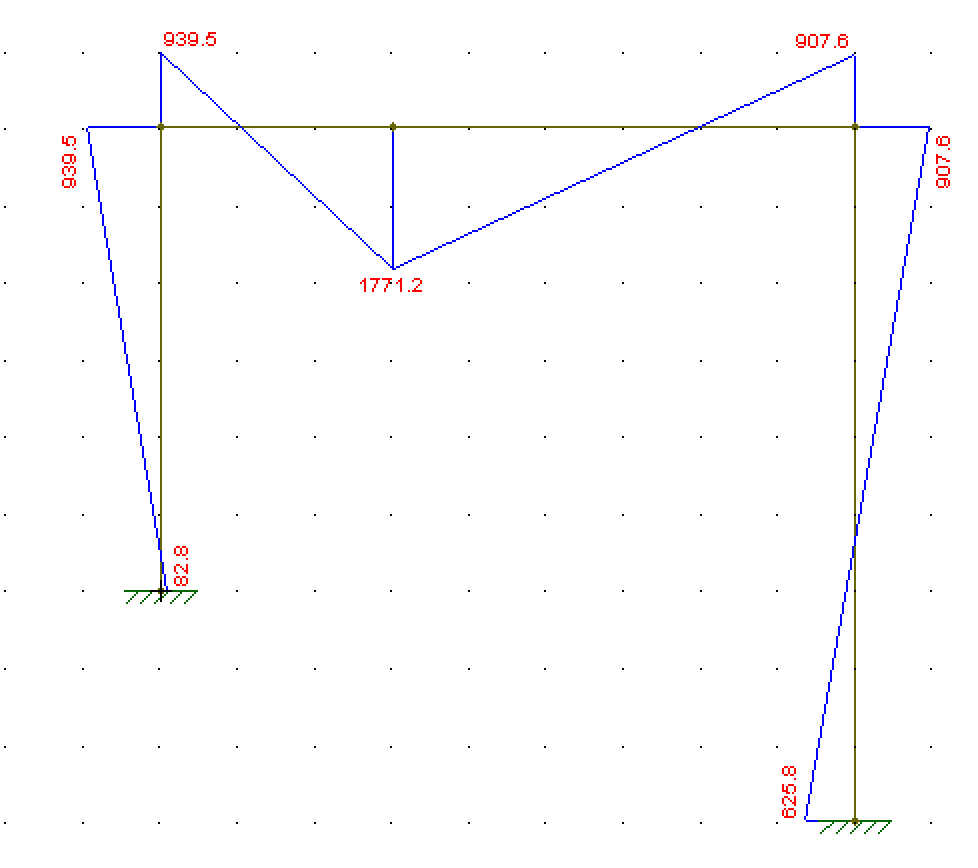
\includegraphics[width=0.53\textwidth]{ejUT3}
	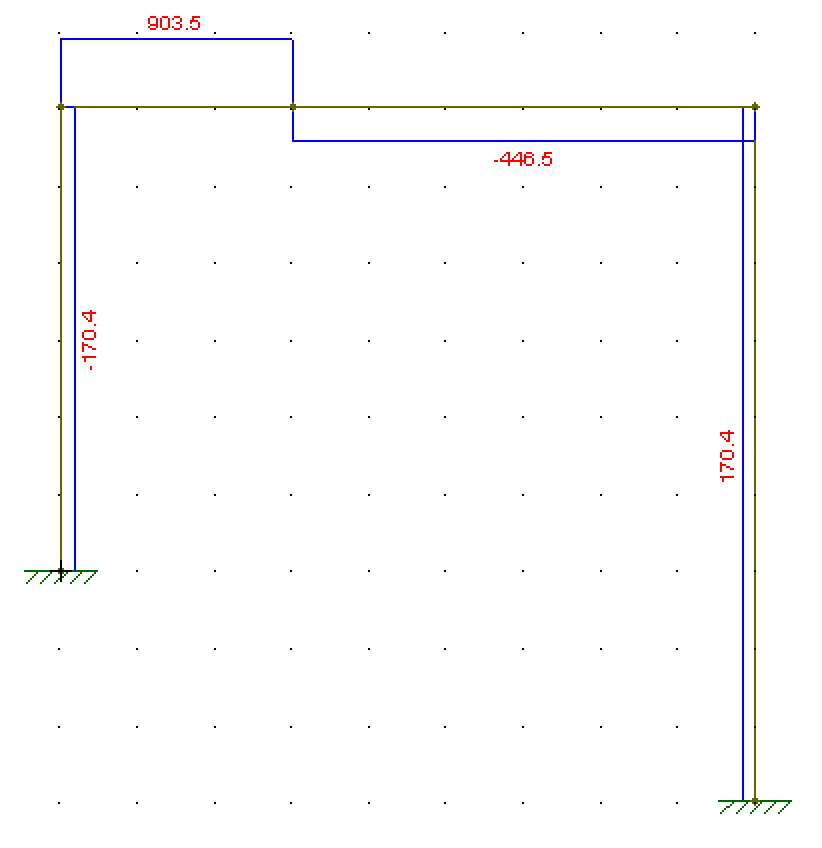
\includegraphics[width=0.45\textwidth]{ejUT3cort}
	\caption{Diagramas de momentos (izquierda) y cortante (derecha).}
	\label{fig:dia1}
\end{figure}

En la \autoref{fig:dia2} se muestran los diagramas de deformada y directas.
\begin{figure}[htb]
	\centering
	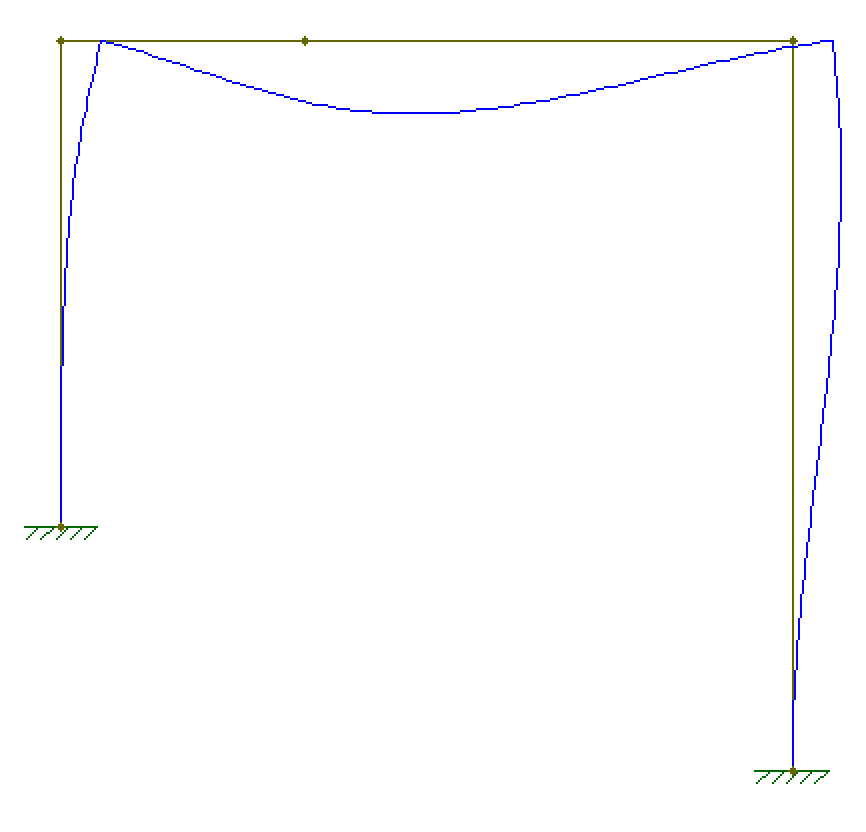
\includegraphics[width=0.45\textwidth]{ejUT3defor}
	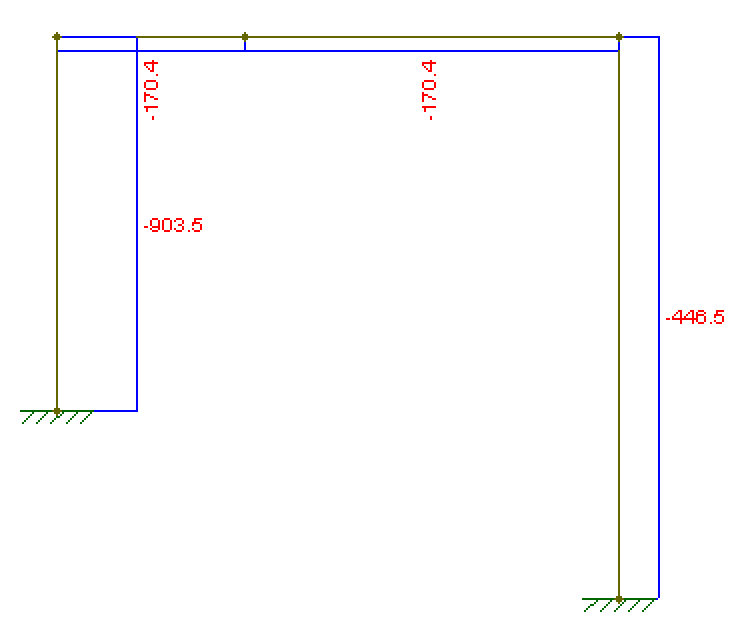
\includegraphics[width=0.53\textwidth]{ejUT3dire}
	\caption{Diagramas de deformada (izquierda) y directas (derecha).}
	\label{fig:dia2}
\end{figure}


\clearpage







\section{Métodos de análisis matricial/computacional}

En esta sección se presentan algunos desarrollos y métodos útiles para comprender el funcionamiento de las herramientas computacionales para el análisis de pórticos planos considerando deformación axial. %
%
Se utiliza un enfoque usualmente utilizado tanto en libros de resistencia de materiales \citep{Pilkey2002} como en libros orientados a métodos computacionales \citep{Onate2013}. %

Se considera una viga bajo las mismas hipótesis establecidas previamente, formada por un material elástico lineal de módulo de Young E sometida a esfuerzos de directa y momento tales que se produce una extensión y flexión. %
%
La expresión de la función de la deformación axial para un punto en $(x,y)$ es:
%
\begin{equation}
\varepsilon_x (x,y) = \varepsilon_G(x) - y \frac{\partial^2 v}{\partial x^2} (x),
\end{equation}
considerando los ejes tal como se muestra en la Figura~\ref{fig:viga3d}. %
%%	
Por otra parte, la tensión axial está dada por:
%
\begin{equation}
\sigma_x (x,y) = E \varepsilon_x(x,y) = E \varepsilon_G(x) - E y \frac{\partial^2 v}{\partial x^2} (x).
\end{equation}

Utilizando estas expresiones y realizando un procedimiento similar al de la Unidad Temática anterior se obtendrán las relaciones entre fuerzas y desplazamientos dadas por el Método de los Desplazamientos en flexión compuesta.

\subsection{Relaciones fuerzas-desplazamiento}

Se considera un elemento de viga con sección transversal uniforme de área $A$ e inercia $I$ de largo $\ell$. %
%
Se considera sometido a fuerzas nodales axiales y transversales y momentos nodales como es mostrado en la Figura~\ref{fig:ejeviga}. %
%
En dicha figura se muestra el eje de la viga en la configuración de referencia con las fuerzas aplicadas y la configuración deformada con los desplazamientos y giros nodales indicados de acuerdo a la convención de signos 2 (ver Figura~\ref{fig:conve}). %
%
\begin{figure}[htb]
	\setlength{\unitlength}{0.8\textwidth}
	\centering
	\def\svgwidth{0.8\textwidth}
	\input{figs/UT4/eje_viga_deformada.pdf_tex}
	\caption{Esquemas de viga: (a) eje de viga en configuración de referencia (línea punteada) y eje de viga deformada (línea continua), (b) eje de viga de referencia con fuerzas aplicadas.}
	\label{fig:ejeviga}
\end{figure}

El desplazamiento de cada nodo de la viga es interpolado a partir de sus desplazamientos y giros nodales, representados en forma vectorial como:
%
\begin{equation}
\bfu = [ u_1, v_1, \theta_1, u_2, v_2, \theta_2 ]^T.
\end{equation}

La energia potencial de deformación de la viga está dada por la expresión:
%
\begin{equation}
\Pi_{int}(\bfu) = \frac{1}{2} \int_{\Omega} E \varepsilon_x (x)^2 \dif V = \frac{1}{2} \int_{\ell} \int_{A} E \left( \varepsilon_G(x) -y \frac{\partial ^2 v}{\partial x^2}(x) \right)^2 \dif A \dif x .
\end{equation}

%
Desarrollando se tiene:
%
\begin{eqnarray}
\Pi_{int}(\bfu) 
&=& \frac{1}{2} \int_{\ell} \int_{A} E \left( \varepsilon_G(x)  \right)^2 \dif A \dif x \nonumber\\
\dots &-&             \int_{\ell} \int_{A} E y \varepsilon_G(x)  \frac{\partial ^2 v}{\partial x^2}(x)  \dif A \dif x \nonumber\\
\dots &+&             \frac{1}{2} \int_{\ell} \int_{A} E y^2 \left(  \frac{\partial ^2 v}{\partial x^2}(x) \right)^2 \dif A \dif x ,
\end{eqnarray}
%
y usando que el origen del sistema de coordenadas es el baricentro de la sección y siendo que la sección transversal es uniforme, se tiene:
%
\begin{equation}
\Pi_{int}(\bfu)  =
\underbrace{ \frac{1}{2} \int_{\ell} \int_{A} E \left( \varepsilon_G(x)  \right)^2 \dif A \dif x }_{\text{axial}}
+  
\underbrace{ \frac{1}{2} \int_{\ell} \int_{A} E y^2 \left(  \frac{\partial ^2 v}{\partial x^2}(x) \right)^2 \dif A \dif x}_{\text{flexión}}.
\end{equation}

En esta expresión fueron definidos los términos de energía de deformación por esfuerzo axial y por esfuerzo de flexión. %
%
Considerando que no existen cargas axiales aplicadas en el tramo del elemento se tiene que la deformación axial del baricentro está dada por:
%
\begin{equation}
\varepsilon_G(x) = \frac{u_2 - u_1}{\ell},
\end{equation}
%
a lo largo de todo el elemento. %
Esto permite expresar las energías en función de los desplazamientos nodales:
%
\begin{equation}
\Pi_{int}(\bfu) = \Pi_{int,\text{axial}}(u_1,u_2) + \Pi_{int,\text{flexión}}(v_1,\theta_1,v_2,\theta_2)
\end{equation}
%
donde la energía de deformación por esfuerzos axiales está dada por:
%
\begin{equation}\label{eqn:Uaxial}
\Pi_{int,\text{axial}}(u_1,u_2) = \frac{1}{2} \frac{E A}{\ell} (u_2 - u_1)^2 
\end{equation}
%
y la energía de deformación por exfuerzos de flexión está dada por:
%
\begin{equation} \label{eqn:Uflex}
\Pi_{int,\text{flexión}} (v_1,\theta_1,v_2,\theta_2) = \frac{1}{2} E I \int_{\ell} \left( \frac{\partial ^2 v}{\partial x^2}(x,v_1,\theta_1,v_2,\theta_2) \right)^2\dif x .
\end{equation}
Nuevamente se recuerda que se está usando que la sección transversal es uniforme.

La energía potencial de las fuerzas externas puede escribirse como:
\begin{equation}
\Pi_{ext} (\bfu) = - \bfu^T \bff
\end{equation}
%
donde $\bff$ es el vector columna de las fuerzas nodales, dado por:
%
\begin{equation}
\bff = [F_{x,1},F_{y,1},M_{1}, F_{x,2},F_{y,2},M_{2} ]^T.
\end{equation}


Se puede obtener por lo tanto la expresión de la energía potencial total:
%
\begin{equation}
\Pi (\bfu) =  \Pi_{int,\text{axial}}(u_1,u_2) + \Pi_{int,\text{flexión}}(v_1,\theta_1,v_2,\theta_2) - \bfu^T \bff
\end{equation}
%
y aplicar las condiciones dadas por el primer teorema de Castigliano:
%
\begin{eqnarray}
\frac{\partial \Pi_{int} }{\partial u_1} = \frac{EA}{\ell} (u_1 - u_2) &=& F_{x,1} \\
%
\frac{\partial \Pi_{int} }{\partial v_1} = EI \left( \dfrac{12}{\ell^{3}} v_1 + \dfrac{6}{\ell^{2}} \theta_1 - \dfrac{12}{\ell^{3}} v_2 + \dfrac{6}{\ell^{2}} \theta_2 \right)  &=& F_{y,1} \\
%
\frac{\partial \Pi_{int} }{\partial \theta_1} = EI \left( \frac{6}{\ell^2} v_1 +  \frac{4}{\ell} \theta_1 - \frac{6}{\ell^2} v_2   + \frac{2}{\ell} \theta_2 \right) &=& M_1 \\
\frac{\partial  \Pi_{int} }{\partial u_2} = \frac{EA}{\ell} (-u_1 + u_2) &=& F_{x,2} \\
%
\frac{\partial \Pi_{int} }{\partial v_2} = EI \left( -\dfrac{12}{\ell^{3}} v_1 - \dfrac{6}{\ell^{2}} \theta_1 +\dfrac{12}{\ell^{3}} v_2 - \dfrac{6}{\ell^{2}} \theta_2 \right) &=& F_{y,2} \\
%
\frac{\partial \Pi_{int} }{\partial \theta_2} = EI \left( \dfrac{6}{\ell^{2}} v_1 + \dfrac{2}{\ell} \theta_1 - \dfrac{6}{\ell^{2}} v_2 + \dfrac{4}{\ell}  \theta_2 \right) &=& M_2.
\end{eqnarray}

Estas condiciones representan la consideración conjunta de las condiciones vistas para la flexión en la Unidad Temática 3 y la deformación axial en la Unidad Temática 2.
%
Esta relación entre desplazamientos nodales y fuerzas puede ser planteada en forma matricial como:
%
\begin{equation}\label{eqn:eqrig}
\bfK \bfu = \bff,
\end{equation}
%
donde la matriz $\bfK$ es la llamada matriz de rigidez:
%
\begin{equation}
\bfK = \left[
\begin{matrix}
\dfrac{EA}{\ell} & 0 & 0 & - \dfrac{EA}{\ell} & 0 & 0 \\[3mm]
%
0 &  12 \dfrac{EI}{\ell^{3}} & 6 \dfrac{EI}{\ell^{2}} &  0& -12 \dfrac{EI}{\ell^{3}} & 6 \dfrac{EI}{\ell^{2}} \\[3mm]
0 &  6 \dfrac{EI}{\ell^{2}} & 4 \dfrac{EI}{\ell} & 0& -6 \dfrac{EI}{\ell^{2}} & 2 \dfrac{EI}{\ell} \\[3mm]
-\dfrac{EA}{\ell} & 0 & 0 &  \dfrac{EA}{\ell} & 0 & 0 \\[3mm]
%
0 &  -12 \dfrac{EI}{\ell^{3}} & -6 \dfrac{EI}{\ell^{2}} &0&  12 \dfrac{EI}{\ell^{3}} & -6 \dfrac{EI}{\ell^{2}} \\[3mm]
0 &  6 \dfrac{EI}{\ell^{2}} & 2 \dfrac{EI}{\ell} & 0 & -6 \dfrac{EI}{\ell^{2}} & 4 \dfrac{EI}{\ell} \\[3mm]
\end{matrix}
\right].
\end{equation}


Es importante destacar que la matriz de rigidez es simétrica, lo que puede ser justificado por el hecho de que la función de energía potencial total es una función de tipo $C^2$ y que la matríz $\bfK$ es la hesiana  de dicha función. %

Por otra parte también se destaca que la matriz $\bfK$ tiene valores propios nulos con sus correspondientes vectores propios asociados. %
(pertenecientes al subespacio asociado al valor propio cero $S_0$). %
%
Esto quiere decir que existen movimientos (dados por los vectores de desplazamientos en dicho subespacio) que se corresponden con fuerzas nodales nulas, por lo tanto estos movimientos no introducen deformaciones o tensiones en el elemento. %
%
Dicho de otra forma, estos movimientos serán los movimientos de cuerpo rígido de la viga. %
%
Estos movimientos son 3 por lo que es necesario eliminar tres grados de libertad (a través de las condiciones de contorno) para obtener una matriz reducida con valores propios positivos y por lo tanto invertible. %
%
De esta forma la solución del sistema es única.

\subsection{Sistemas de coordenadas y análisis matricial}

Para encontrar la relación entre desplazamientos y fuerzas nodales en problemas de pórticos donde los ejes de los elementos que concurren a un nodo no coinciden, es útil definir un sistema de coordenadas global de la misma forma en que fue realizado para reticulados planos.
%

En el caso de pórticos el cambio de base se aplica a los desplazamientos nodales, mientras que los giros se mantienen en el mismo versor de referencia. %
%
La matriz de cambio de base esta dada por
%
\begin{equation}
\bfR^e = 
\left[
\begin{matrix}
c & -s & 0 & 0 &  0 & 0 \\
s & c & 0 & 0 &  0 & 0\\
0 & 0 &1 & 0 &  0 & 0\\
0 & 0 &0  &   c & -s& 0\\
0 & 0 &0  &  s & c & 0\\
0 & 0 &0 & 0 &  0 & 1\\
\end{matrix}
\right]
\qquad
\bfu^e = \bfR^e \bfu^e_L
\end{equation}
%
donde $c=\cos(\alpha^e)$ y $s=\sin(\alpha^e)$ y $\alpha^e$ es el ángulo medido positivo antihorario desde el eje global al local. %
%
La Ecuación~\eqref{eqn:eqrig} fue desarrollada en coordenadas locales utilizando la notación $\bfu$, la cual en el caso de sistemas coordenadas locales y globales correspondería a los ejes locales, por lo que debería ser escrita como
\begin{equation}
\bfK_L \bfu_L = \bfF_L.
\end{equation}
%
La matriz de rigidez en coordenadas globales está dada por:
\begin{equation}
\bfK^e_G = \bfR^e \bfK^e_L (\bfR^e)^T
\end{equation}

%
El sistema global obtenido luego de realizado el ensamblado es denotado por:
\begin{equation}
\bfK_G \bfu = \bfF_G.
\end{equation}
donde $\bfF_G$ es el vector de fuerzas externas nodales en coordenadas globales.

La determinación de desplazamientos a través del ensamblado de un sistema de ecuaciones lineales es llamado Análisis Matricial dado que se realiza a través del ensamblado e inversión de matrices de dimensiones considerables. %
%
La aplicación de este método para estructuras con cargas nodales es equivalente al MEF utilizando elementos de pórtico (\textit{frame} en inglés) \citep{Onate2013}, procedimiento utilizado por la mayoría de los programas computacionales de determinación de solicitaciones.

\subsection{Apoyos elásticos}

Para la resolución mediante análisis matricial o  de forma computacional, las fuerzas introducidas por los resortes pueden ser consideradas a través de una matriz de rigidez para cada elemento (en coordenadas globales):
\begin{equation}
\bfK_S^e = 
\left[
\begin{matrix}
k_{u1} & 0 & 0 & 0 &  0 & 0 \\
0 & k_{v1} & 0 & 0 &  0 & 0\\
0 & 0 &k_{\theta1} & 0 &  0 & 0\\
0 & 0 &0  &   k_{u2} & 0& 0\\
0 & 0 &0  &  0 & k_{v2} & 0\\
0 & 0 &0 & 0 &  0 & k_{\theta2}\\
\end{matrix}
\right]
\end{equation}
que puede ser ensamblada y sumada a la matriz de rigidez global, obteniendo un sistema dado por
%
\begin{equation}
\left(\bfK_G + \bfK_S \right) \bfu = \bfF_G.
\end{equation}

\subsection{Comparación de energías de deformación}

Tal como fue visto en la Unidad Temática 3, para la aplicación de métodos analíticos como el método de Slope-deflection, es usual considerar que la energía de deformación por directa es despreciable respecto a la de flexión. Esto permite eliminar algunas incógnitas cinemáticas. %

Esta hipótesis es adecuada si se cumple:
%
\begin{equation}
\Pi_{int,\text{axial}} \ll \Pi_{int,\text{flexión}}
\end{equation}
%
lo que es equivalente a:%
%
\begin{equation}
\frac{1}{2} \int_{0}^{\ell} E A  \varepsilon_G^2 \dif x \ll \frac{1}{2} \int_{0}^{\ell} EI \left( \frac{\partial^2 v}{\partial x^2}\right)^2 \dif x
\end{equation}
usando las expresiones obtenidas en la unidad temática 3: 
\begin{equation}
\varepsilon_G(x) = \frac{	N (x) }{E A}
\quad
\text{y}
\quad
\frac{\partial^2 v}{\partial x^2}(x) = \frac{	M (x) }{E I} ,
\end{equation}
se tiene que esa condición es equivalente a 
%
\begin{equation}
\int_{0}^{\ell} \frac{	N (x)^2 }{E A} \dif x \ll \int_{0}^{\ell} \frac{	M (x)^2 }{E I}  \dif x.
\end{equation}



\subsection{Método de Elementos Finitos}

El Método de Elementos Finitos (MEF) puede también ser considerado un método de desplazamientos ya que las incógnitas principales son desplazamientos y giros. %
%
Por otra parte, el enfoque del método permite obtener las ecuaciones que gobiernan la deformación de diversos elementos estructurales \citep{Onate2013}.

Se pueden enumerar algunas diferencias centrales respecto a los métodos analíticos.
%
\begin{itemize}
	\item Para cargas puntuales aplicadas en el tramo, en el MEF se suele dividir el elemento de viga en dos elementos, agregando un nodo en el punto de aplicación de la carga. Esto aumenta la cantidad de variables, lo cual no es relevante dado que el sistema lineal es resuelto numéricamente, y también simplifica la implementación del método.
	%
	\item Las cargas distribuidas suelen ser consideradas discretizando el elemento en un número apropiado de elementos finitos agregando nodos intermedios y por lo tanto más incógnitas del problema. De esta forma se pueden calcular los diagramas de solicitaciones aproximados de forma directa. % 
	Se debe también tener en cuenta que las solicitaciones no necesariamente serán exactas dentro del dominio de cada elemento, dado que existen aproximaciones por la interpolación considerada.
	%
	\item En el MEF es posible automatizar la verificación de estabilidad del esquema básico estructural considerado, a través del análisis de los valores propios de la matriz de rigidez ensamblada y con las condiciones de contorno aplicadas. %
	%
	Esto permite automatizar esa verificación, considerada muy importante al obtener solicitaciones de estructuras de grandes dimensiones \citep{Kannan2014}. 
\end{itemize}

En este curso no se mencionan aspectos sobre la convergencia de las soluciones al aumentar la cantidad de elementos finitos, el estudiante interesado puede consultar \citep{Hughes1987a}.

El ONSAS es un ejemplo de herramienta numérica basada en el método de los elementos finitos.

%
%\subsubsection{Comparación MSD, MEF y soluciones analíticas}
%
%Los métodos MSD y MEF son derivados a partir de las mismas ecuaciones y ambos son métodos de desplazamientos. %
%Sin embargo se puede decir que una diferencia a tener en cuenta es la cantidad de incógnitas a determinar. %
%%
%En el MSD las cargas en el tramo son incluidas a través del vector de fuerzas nodales mientras que en el MEF se suelen agregar nodos intermedios. %
%% 
%
%








\section{Ejercicios}
\setcounter{ejercicio}{0}

En cada ejercicio o estructura descrita a continuación, se pide:
%
\begin{enumerate}
  \item Identificar la mínima cantidad de incógnitas a hallar para obtener las solicitaciones de la estructura mediante el método de Slope Deflection.
  \item  Encontrar las ecuaciones que permiten resolver dichas incógnitas.
  \item  Calcular reacciones y trazar diagramas de solicitaciones.
  \item  Modelar las estructuras en un programa computacional y comparar resultados.
\end{enumerate}

\ejercicio

La viga de madera de la figura ($E=10$ GPa), compuesta por una escuadría de $20$ cm $\times$ $40$ cm.

\begin{center}
	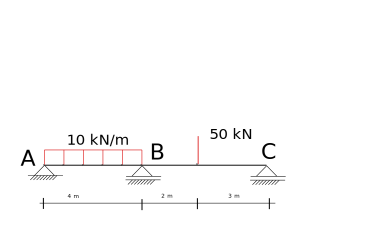
\includegraphics[width=0.9\linewidth]{UT3ej1}
\end{center}


\ejercicio

La estructura de acero de la figura ($E=210$ GPa), compuesta por una viga (ABC) formada por 1 PNI28 y un pilar (BD) formada por un perfil PNI22.

\begin{center}
	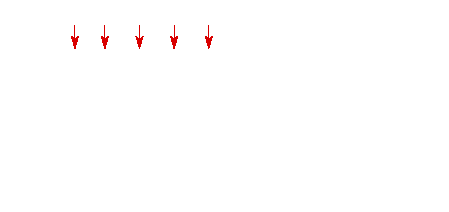
\includegraphics[width=0.6\linewidth]{UT3ej2}
\end{center}


\ejercicio

La estructura de acero ($E=210$ GPa) compuesta por una viga (ABC), dos pilares (AD y BE) y un tensor (BD), cuya sección es 1PNI18.

\begin{center}
	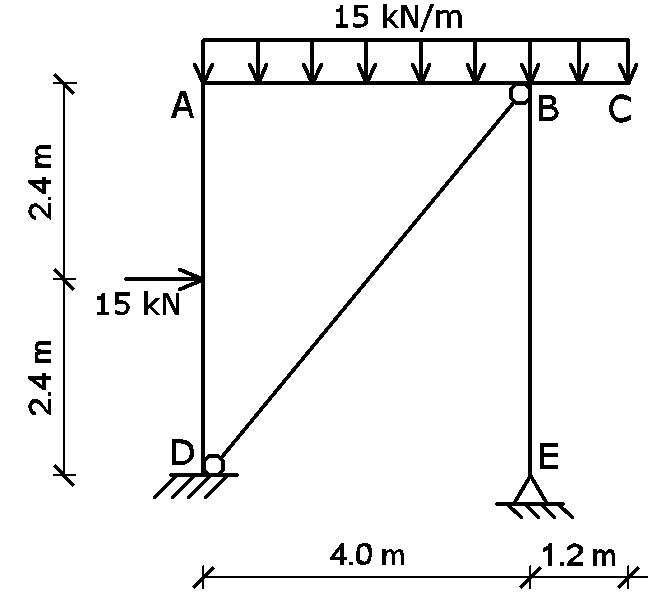
\includegraphics[width=0.5\linewidth]{UT3ej3}
\end{center}

\ejercicio

En la estructura de hormigón de la figura (E=25 GPa) los pilares son de 20x30 cm mientras que la viga es de 15x40 cm. 

\begin{center}
	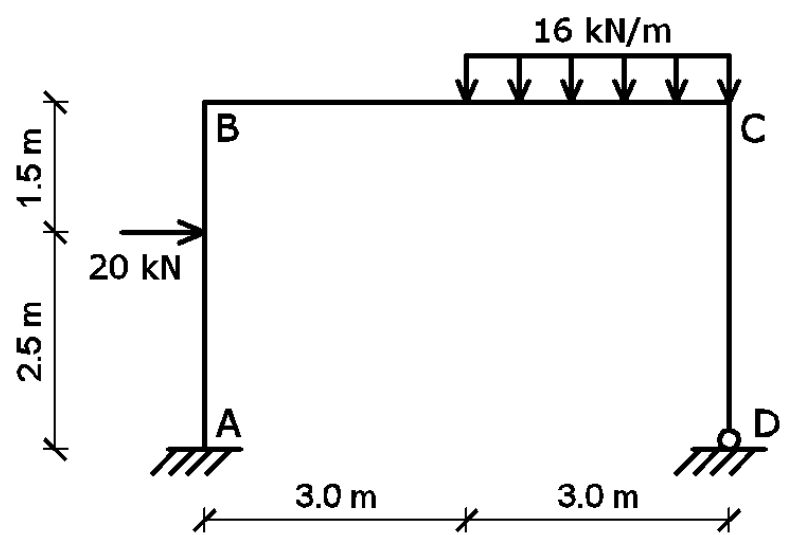
\includegraphics[width=0.65\linewidth]{UT3ej4}
\end{center}


\ejercicio

En la estructura de acero de la figura (E=210 GPa), las barras BD, CF y DE están conformadas por 2PNC24 soldados ([]), mientras que la barra AB está compuesta por 1PNI20. 


\begin{center}
	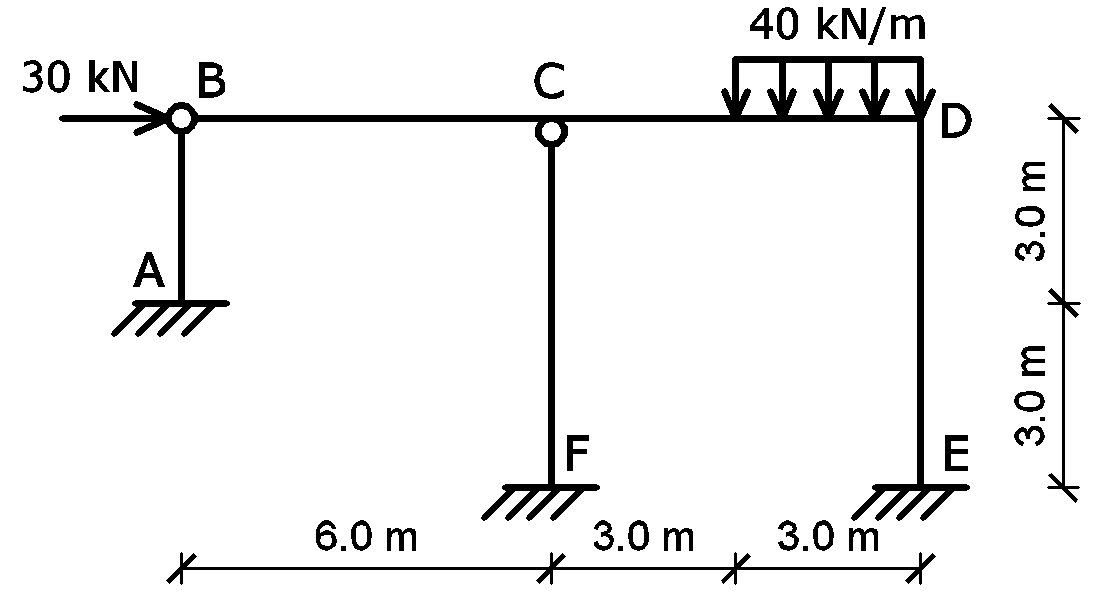
\includegraphics[width=0.75\linewidth]{UT3ej5}
\end{center}



\ejercicio 

En la estructura de hormigón de la figura (E=30 GPa) las secciones son rectangulares de 12x30 cm. 

\begin{center}
	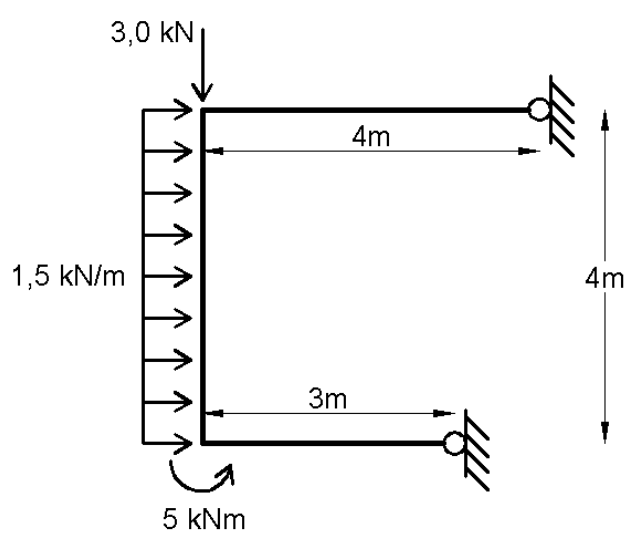
\includegraphics[width=0.6\linewidth]{UT3ej6}
\end{center}


\ejercicio


Sean las siguientes estructuras conformadas por barras de \textbf{EI}=cte y de longitud \textbf{L} sometidas a un desplazamiento impuesto $\Delta$. Se pide calcular los momentos flectores en los empotramientos.


\begin{center}
	\def\svgwidth{0.45\textwidth}
	a) \input{figs/UT3/UT3ejDespa.pdf_tex}
	\def\svgwidth{0.45\textwidth}
	b) \input{figs/UT3/UT3ejDespb.pdf_tex}
\end{center}

% codigoFuenteLibroR2
% Copyright (C) 2020  J.M. Perez Zerpa, et. al.
%
% This program is free software: you can redistribute it and/or modify
% it under the terms of the GNU General Public License as published by
% the Free Software Foundation version 3 of the License.
%
% This program is distributed in the hope that it will be useful,
% but WITHOUT ANY WARRANTY; without even the implied warranty of
% MERCHANTABILITY or FITNESS FOR A PARTICULAR PURPOSE. See the
% GNU General Public License for more details.
%
% You should have received a copy of the GNU General Public License
% along with this program.  If not, see <http://www.gnu.org/licenses/>.

\chapter[Simetría y Líneas de Influencia en pórticos]{Simetría y Líneas de Influencia en pórticos}


En esta unidad se presentan dos conceptos o métodos específicos del análisis de pórticos planos.  Por una parte simetría y antisimetría, con su aplicación al análisis simplificado de pórticos planos. Por otra parte se presenta una introducción a la aplicación de líneas de influencia en pórticos hiperestáticos. %
%
Para la sección de simetría se utiliza un enfoque basado en las ecuaciones de equilibrio para obtener las condiciones mecánicas y cinemáticas dadas por la simetría, aplicándolas luego en pórticos de forma similar a como es realizado en \citep{CerveraRuiz2002ii}. %
%
La sección de Líneas de Influencia está basada en \citep{Celigueta2003}.




\section{Simetría en estructuras planas}

En esta sección se desarrollan los puntos más importantes para la consideración de simetría en el análisis de pórticos. %
%
Para la presentación se consideran pórticos planos cuya geometría tiene un eje de simetría axial. %
%
Los conceptos vistos pueden ser generalizados a estructuras tridimensionales.

\subsection{Viga sometida a cargas externas simétricas}

En la \autoref{fig:vigsim} se muestra un elemento de viga con sección transversal con inercia $I$ y área $A$, módulo de Young $E$ y largo $\ell$, el cual está sometido a cargas distribuidas y nodales simétricas respecto al punto medio de la viga (punto considerado como origen de la coordenada $x$). %

\begin{figure}[htb]
\centering
\def\svgwidth{0.9\textwidth}
\input{figs/UT4/vigasime.pdf_tex}
\caption{Esquema de viga sometiga a cargas simétricas.}
\label{fig:vigsim}
\end{figure}

Las cargas nodales pueden ser provocadas por agentes externos o bien deberse a reacciones asociadas a vínculos que restringen desplazamientos nodales. %
%
Si las cargas y las restricciones en desplazamiento (vínculos a tierra) son simétricos entonces las reacciones asociadas a dichos vínculos también lo serán. %

Se desea obtener cuales son las propiedades que cumplen las solicitaciones y los desplazamientos para este caso. %
%
Para esto se plantean las expresiones matemáticas de cada una de las hipótesis y ecuaciones disponibles y se procede a realizar el desarrollo.

\paragraph{Simetría de cargas externas}
%
Observando en la figura la simetría de las fuerzas nodales y recordando la convención de signos de la UT3 para solicitaciones internas, se tiene que la simetría es equivalente a las siguientes condiciones en las solicitaciones en los extremos:
%
\begin{eqnarray}
V \left(-\frac{\ell}{2}\right) = F_y \quad 
V\left( \frac{\ell}{2}\right) = -F_y \\
M\left( -\frac{\ell}{2}\right) = M_n \quad
M\left( \frac{\ell}{2} \right) = M_n.
\end{eqnarray}
%

Por otra parte, la simetría de la carga distribuida es equivalente a decir que la función de la carga $q(x):\left[-\frac{\ell}{2},\frac{\ell}{2} \right] \rightarrow \bbR$ es una función par. %
%
La definición de función par establece que:
\begin{equation}
q( x) = q(-x) \qquad \forall x \in \left[-\frac{\ell}{2},\frac{\ell}{2} \right].
\end{equation}

Estas relaciones representan condiciones de contorno para obtener relaciones particulares a partir de las ecuaciones de equilibrio.

\paragraph{Equilibrio puntual y relación con desplazamientos}
Se pasa a analizar la forma de las ecuaciones de equilibrio puntual, dadas por:
\begin{eqnarray}
\frac{dV}{d x} &=& q \\
\frac{dM}{d x} &=& V
\end{eqnarray}
donde nuevamente se recuerda que se utiliza la convención de signos 1 de la UT3. También se cuenta con las relaciones fuerza desplazamiento obtenidas en la UT3 a partir de la ecuación constitutiva y las hipótesis cinemáticas:
\begin{eqnarray}
\frac{d\theta}{d x} &=& \frac{M}{E I} \\
\frac{dv}{d x} &=& \theta
\end{eqnarray}



\paragraph{Equilibrio global}
Finalmente se establece la condición del equilibrio global para cualquier segmento de viga considerado. %
%
En particular se consideran las dos mitades de la viga por lo que se realiza un corte en $x=0$. %
%
El equilibrio de fuerzas verticales de la mitad derecha está dado por:
%
\begin{equation}\label{eqn:vmas}
  V(0) + \int_{0}^{\ell/2} q(u) du + F_y = 0
\end{equation}
%
donde $V(0)$ es el cortante en la sección del plano de simetría., %
%
Por otra parte también se tiene la ecuación del equilibrio de fuerzas de la mitad izquierda, dado por:
%
\begin{equation}\label{eqn:vmenos}
  -V(0) + \int_{-\ell/2}^0 q(u) du + F_y = 0.
\end{equation}
%

Considerando el cambio de variable $s=-u$ y usando que $q$ es par se tiene:
\begin{equation}
-V(0) - \int_{\ell/2}^0 q(s) ds + F_y = 0
\end{equation}
invirtiendo los límites de integración se obtiene
%
\begin{equation}
-V(0) + \int_{0}^{\ell/2} q(s) ds + F_y = 0
\end{equation}
Restando miembro a miembro la Ecuación~\eqref{eqn:vmas} se tiene
\begin{equation}\label{eqn:vex}
-V(0) - V(0) = 0\Rightarrow  \boxed{
	V(0) = 0}.
\end{equation}

% --------------------------


\paragraph{Desarrollo de cortante}
Se pasa a buscar cual es la forma del cortante $V(x)$ bajo las hipótesis consideradas. %
%
El cortante puede ser calculado integrando la primer ecuación puntual de equilibrio:
%
\begin{equation}
V(x) = \int_{0}^{x} q(u) \dif u + V(0).
\end{equation}
%
Es importante destacar que esta ecuación es equivalente a considerar el equilibrio de fuerzas verticales del segmento de viga $[0,x]$.


Usando el resultado de la Ecuación~\eqref{eqn:vex} se tiene:
\begin{equation}\label{eqn:v1}
V(x) = \int_{0}^{x} q(u) \dif u.
\end{equation}

Considerando el cambio de variable $s=-u$ se obtiene:
%
\begin{equation}
V(x) = \int_{0}^{-x} -q(-s) \dif s,
\end{equation}
%
donde se puede nuevamente ver que esto es equivalente a una ecuación de equilibrio del segmento $[-x,0]$. %
Usando que $q$ es par se tiene
\begin{equation}\label{eqn:v2}
V(x) = - \int_{0}^{-x} q(s) \dif s.
\end{equation}
%


A partir de las ecuaciones \eqref{eqn:v1} y \eqref{eqn:v2} se puede ver que:
%
\begin{equation}
V(x) = - \int_{0}^{-x} q(s) \dif s  = -V(-x)
\Rightarrow \boxed{
V(x) = -V(-x)}
\end{equation}
%
por lo que queda demostrado que $V$ es una función impar y el cortante es nulo en el eje de simetría.


\paragraph{Desarrollo de momento}
El momento interno en una sección cualquiera $x$ puede ser obtenido  a partir de la segunda ecuación puntual de equilibrio:
%
\begin{equation}
M(x) = \int_{0}^{x} V(u) \dif u + M(0).
\end{equation}
%
Realizando el cambio de variable $s=-u$ se obtiene
\begin{equation}
M(x) = \int_{0}^{-x} -V(-s) \dif s + M(0)
\end{equation}
%
y usando que $V$ es impar se tiene
\begin{equation}
M(x) = \int_{0}^{-x} V(s) \dif s + M(0) = M(-x)
\Rightarrow \boxed{
M(x) = M(-x)
}
\end{equation}
por lo que se demostró que $M$ es par.

\paragraph{Desarrollo de giro}
El giro puede ser calculado integrando la ecuación de momento curvatura:
%
\begin{equation}
\theta(x) = \int_{0}^{x} \frac{ M(u)}{EI} \dif u + \theta(0).
\end{equation}
%
Haciendo cambio de variable $s=-u$ y usando que el momento es par se obtiene:
\begin{equation}
\theta(x) = - \int_{0}^{-x} \frac{ M(s)}{EI} \dif s + \theta(0).
\end{equation}

Si se considera cada mitad de la viga por separado se puede ver que el giro del punto en el eje de simetría debería tener valores opuestos debido a la simetría de las cargas. %
%
Por otra parte por continuidad de la viga en dicho punto se cumple que los giros de ambos extremos deben ser iguales por lo que se concluye que dicho giro debe de ser nulo, por lo tanto $\theta(0) = 0$. 

Se tiene por lo tanto que:
%
\begin{equation}
  \theta(x) = - \int_{0}^{-x} \frac{ M(s)}{EI} \dif s =  -\theta(-x) \Rightarrow \boxed{\theta(x) = -\theta(-x)}.
\end{equation}
por lo que se demostró que el giro es impar y tiene valor nulo en el eje de simetría.

\paragraph{Desarrollo de flecha}
La flecha se obtiene integrando la ecuación diferencial que la relaciona con el giro:
%
\begin{equation}
v(x) = \int_{0}^{x} \theta(u) \dif u + v(0).
\end{equation}
%
Realizando el cambio de variable $s=-u$ se obtiene
\begin{equation}
v(x) = \int_{0}^{-x} -\theta(-s) \dif s + v(0)
\end{equation}
y usando que el giro es impar se tiene
\begin{equation}
v(x) = \int_{0}^{-x} \theta(s) \dif s + v(0) = v(-x)
\Rightarrow \boxed{
	v(x) = v(-x)
}
\end{equation}
por lo que se demostró que $v$ es par.

En resumen se probó que para las hipótesis establecidas, si la \textbf{carga} distribuida par $q(x) = q(-x)$ se cumple que: 
\begin{itemize}
	\item el \textbf{cortante} impar $V(x) = -V(-x)$,
	\item el \textbf{momento} par $M(x) = M(-x)$,
	\item el \textbf{giro} impar $\theta(x) = -\theta(-x)$,
	\item y la \textbf{flecha} par $v(x) = v(-x)$.
\end{itemize}


\subsubsection{Carga puntual o articulación en eje de simetría}

De forma análoga se pueden desarrollar las variantes de las ecuaciones para los casos en los que existe una carga puntual o una articulación en el eje de simetría de la viga.

En el caso de carga puntual existe una discontinuidad antisimétrica en el cortante de valor igual a la carga aplicada y en el caso de la articulación existen también una discontinuidad impar del valor del giro a cada lado de la articulación. %
%


\subsection{Pórticos planos simétricos con cargas simétricas}

El mismo razonamiento realizado para vigas puede ser extendido a pórticos, donde se debe considerar un sistema de coordenadas local $x$ continuo a lo largo de los pilares y vigas que se deseen analizar en cada etapa. %
%
El estudiante interesado en comprender en mayor profundidad el enfoque utilizado puede consultar \citep{CerveraRuiz2002ii}. %

En caso de existir una barra en el eje de simetría se obtiene un resultado equivalente al obtenido considerando una barra con la mitad de rigidez a directa, es decir con una sección transversal con la \textit{mitad de área}. %
%



En la \autoref{fig:simplifporsim} se muestra a la izquierda un pórtico simétrico con cargas simétricas aplicadas y a la derecha un pórtico equivalente obtenido a partir de las consideraciones de simetría y los resultados obtenidos. %
%
\begin{figure}[htb]
\centering
\def\svgwidth{0.8\textwidth}
\input{figs/UT4/simeport.pdf_tex}
\caption{Esquema de simplificación por consideraciones de simetría de pórtico.}
\label{fig:simplifporsim}
\end{figure}

Es importante destacar en este caso que el empotramiento deslizante considerado en el eje de simetría está asociado al hecho de que el giro es nulo por la simetría de las cargas y no necesariamente a la rigidez a flexión del pilar del eje de simetría.


\subsection{Viga simétrica con cargas externas antisimétricas}

En esta sección se presentan de forma sintética las condiciones correspondientes a estructuras \textbf{simétricas} con cargas antisimétricas (es decir impares). %

De forma análoga al caso de la viga con cargas simétricas, si las cargas son antisimétricas se cumple que:
%
\begin{itemize}
\item \textbf{carga} distribuida impar $q(x) = -q(-x)$
\item \textbf{cortante} par $V(x) = V(-x)$
\item \textbf{momento} impar $M(x) = -M(-x)$
\item \textbf{giro} par $\theta(x) = \theta(-x)$
\item \textbf{flecha} impar $v(x) = -v(-x)$
\end{itemize}

Se puede mostrar que el momento es nulo en el eje de simetría.

\subsection{Pórticos planos simétricos con cargas antisimétricas}

%Se puede mostrar que en el caso de pórticos simétricos sometidos a cargas antisimétricas se aplican consideraciones similares a las anteriores. %
%
En la \autoref{fig:simpanti} se muestra a la izquierda un pórtico con cargas antisimétricas y a la derecha un pórtico obtenido a partir de las simplificaciones de antisimetría consideradas.
%
\begin{figure}[htb]
	\centering
	\setlength{\unitlength}{0.8\textwidth}
\def\svgwidth{0.8\textwidth}
\input{figs/UT4/antisimeport.pdf_tex}
	\caption{Esquema de simplificación por consideraciones de antisimetría de pórtico.}
	\label{fig:simpanti}
\end{figure}

Es importante destacar en este caso que el apoyo deslizante considerado en el eje de simetría está asociado al hecho de que la flecha es nula por la antisimetría de las cargas y no necesariamente a la rigidez a directa del pilar del eje de simetría.

\subsection{Descomposición simetría/antisimetría}

En práctico se mostrará que, para una estructura simétrica, es posible descomponer cualquier estado de carga en suma de uno simétrico y otro antisimétrico, permitiendo simplificar el análisis de cualquier estructura simétrica.


\section{Líneas de influencia}

En esta sección se presenta un método para la determinación de líneas de influencia de reacciones y solicitaciones en estructuras hiperestáticas. %
%
El enfoque utilizado se basa en la aplicación de superposición y el Teorema de Betti (enunciado en la Sección~\ref{sec:Betti}).
%
El texto de referencia utilizado es \citep{Celigueta2003}.


Se asume que los conceptos de línea de influencia son conocidos y que se conocen los métodos utilizados para determinar las líneas de influencia en reticulados y vigas isostáticas. %
%
En caso de no contar con estos conceptos, se sugiere consultar el capítulo 10 del texto referenciado previo a leer esta sección.


Para presentar los métodos para determinación de las distintas solicitaciones se utilizará un ejemplo mostrado en la Figura~\ref{fig:ejemLI}. %
%
El esquema básico considerado consiste en un pórtico formado por elementos de pórtico de rigidez a flexión uniforme $EI$ con cuatro nodos como se muestra en la figura.

\begin{figure}[htb]
	\centering
	\def\svgwidth{0.65\textwidth}
  \input{figs/UT4/UT4_ejemploLInf_planteo.pdf_tex}
  \caption{Esquema básico de cálculo de ejemplo de líneas de influencia.}
	\label{fig:ejemLI}
\end{figure}

La flecha con un círculo representa la carga aplicada considerada móvil, en todo el tramo horizontal de la estructura y de módulo unitario.

\subsection{Líneas de influencia de reacciones}

Si se desea calcular por ejemplo la reacción vertical del nodo 3, se debe liberar el grado de libertad cinemático correspondiente. %
%
Esto es, modificar el apoyo fijo del nodo 3 por un apoyo deslizante vertical, como se muestra en la Figura~\ref{fig:ejemLIRv3}.
%

\begin{figure}[htb]
	\centering
	\def\svgwidth{0.9\textwidth}
	\input{./figs/UT4/UT4EjemploLInfRy3.pdf_tex}
	\caption{Esquemas de estados para determinación de línea de influencia de reacción.}
	\label{fig:ejemLIRv3}
\end{figure}

Los desplazamientos de cada estado son representado como $\Delta^I_{y,3}$ y $\Delta^{II}_{y,3}$ y el desplazamiento de la estructura real es calculado como
\begin{equation}
  \Delta_{y,3} = \Delta_{y,3}^I + R_{y,3} \Delta_{y,3}^{II}.
\end{equation}

La condición de apoyo fijo en 3 es $\Delta_{y,3}=0$, por lo que imponiendo esto, se puede obtener el valor de la reacción deseada:
%
\begin{equation}\label{eqn:Ry3}
  R_{y,3} = - \frac{\Delta_{y,3}^I}{ \Delta_{y,3}^{II}}.
\end{equation}

Para poder obtener un método simple de cálculo, se debe poder calcular el desplazamiento del estado I de otra forma. Para esto, se utiliza el Teorema de Betti, el cual permite establecer una relación entre el trabajo de las cargas del estado I con los desplazamientos del estado II y las cargas del estado II y los desplazamientos del estado I.

La relación establecida por el Teorema de Betti es:
%
\begin{equation}
1 \Delta_{y,P}^{II} = 1 \Delta_{y,3}^{I},
\end{equation}
donde $P$ es el punto variable de aplicación de la carga. %
%
Sustituyendo en la Ecuación~\eqref{eqn:Ry3} se tiene:
%
\begin{equation}
\boxed{
R_{y,3} = - \frac{\Delta_{y,P}^{II}}{ \Delta_{y,3}^{II}},
}
\end{equation}
%
expresión que permite calcular la línea de influencia realizando el análisis de un único EBC con un único estado de cargas estáticas.
%
En los materiales complementarios audiovisuales se mostrarán los diagramas utilizando herramientas computacionales y los desarrollos analíticos correspondientes.


\subsection{Líneas de influencia de cortantes}

Para calcular líneas de influencia de cortantes se debe liberar el vínculo cinemático correspondiente, es decir la continuidad de desplazamiento transversal.

Se considera que se desea calcular la línea de influencia del cortante (solicitación interna), en el punto medio del tramo $\circled{1}-\circled{2}$, llamado M. Para esto se libera la continuidad y se consideran los estados o esquemas básicos de cálculo mostrado en la Figura~\ref{fig:ejemLIVM}. 

\begin{figure}[htb]
	\centering
	\def\svgwidth{0.9\textwidth}
	\input{figs/UT4/EjemploLInfVM.pdf_tex}
	\caption{Esquemas de estados para determinación de línea de influencia de cortantes.}
	\label{fig:ejemLIVM}
\end{figure}

$\Delta_{y,Mi}$ y $\Delta_{y,Md}$ representan los desplazamientos transversales a la izquierda y derecha del empotramiento deslizante considerado. %
%
La condición de continuidad del desplazamiento transversal está dada por:
%
\begin{equation}\label{eqn:contDelta}
\Delta_{y,Mi} = -\Delta_{y,Md}
\end{equation}

Por otra parte, utilizando superposición, los desplazamientos en la estructura \textit{real} (con el valor de cortante $V_M$ a determinar), pueden ser escritos como:
%
\begin{eqnarray}
\Delta_{y,Mi} &=& \Delta_{y,Mi}^I + V_M \Delta_{y,Mi}^{II} \\
\Delta_{y,Md} &=& \Delta_{y,Md}^I + V_M \Delta_{y,Md}^{II} 
\end{eqnarray}

Sustituyendo en la condición de continuidad de la Ecuación~\eqref{eqn:contDelta}, se tiene:
%
\begin{equation}
\Delta_{y,Mi}^I + V_M \Delta_{y,Mi}^{II} = - \left( \Delta_{y,Md}^I + V_M \Delta_{y,Md}^{II}  \right)
\end{equation}

Por lo tanto, el cortante que garantiza la continuidad está dado por:
%
\begin{equation}
V_M  =  - \frac{ \Delta_{y,Mi}^I + \Delta_{y,Md}^{I} } { \Delta_{y,Mi}^{II} + \Delta_{y,Md}^{II} } 
\end{equation}


Usando el Teorema de Betti se tiene:
\begin{equation}
1 \cdot \Delta_{y,Mi}^I + 1\cdot  \Delta_{y,Md}^{I} = 1\cdot  \Delta_{y,P}^{II} 
\end{equation}

por lo tanto el cortante puede ser calculado como:
%
\begin{equation}
\boxed{
V_M  =  - \frac{ \Delta_{y,P}^{II}  } { \Delta_{y,Mi}^{II} + \Delta_{y,Md}^{II} } 
}
\end{equation}

En los videos complementarios se presentarán ejemplos del cálculo de líneas de influencia de cortantes.

\subsection{Líneas de influencia de momentos}

En el material complementario audiovisual se presentará el procedimiento de aplicación de \textit{Betti} para el cálculo de líneas de influencia de momentos flectores, así como también ejemplos.


\section{Ejercicios}
\setcounter{ejercicio}{0}

En todos los ejercicios presentados a continuación se deberá trabajar con estructuras simplificadas a través del uso de la simetría o antisimetría cuando corresponda, así como también, resortes equivalentes para algunas componentes estructurales. %
%



\ejercicio 

En la estructura de acero ($E=210$ GPa) de la figura, la viga continua AE está conformada por 2 PNC 18 soldados ([]) y cada uno de los tensores BF y DG tiene una sección transversal constituida por 2 barras $\phi$16. 

\begin{center}
	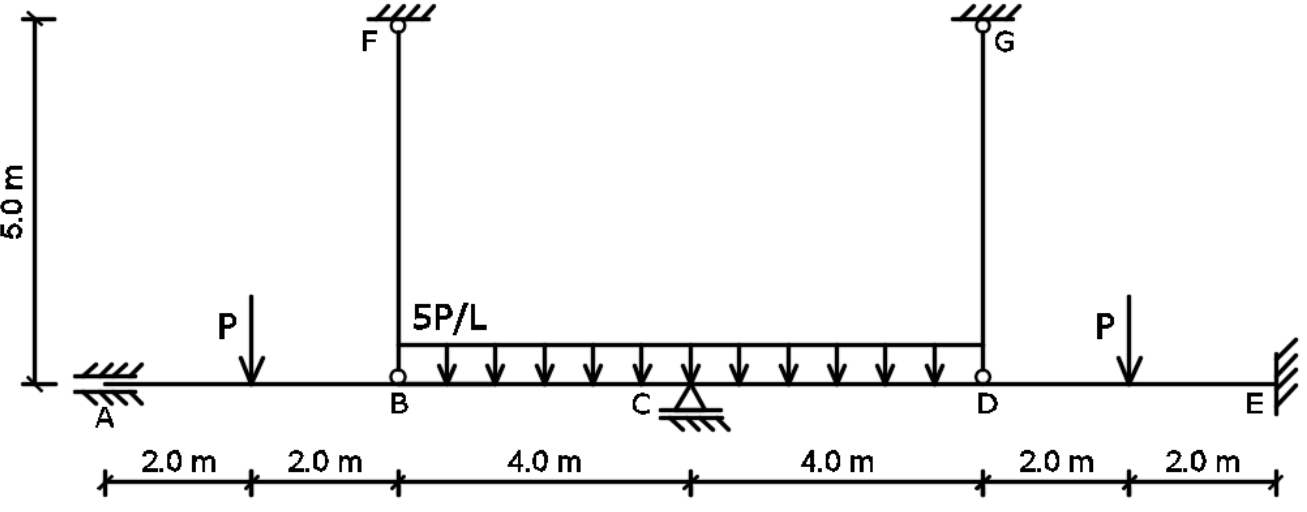
\includegraphics[width=\linewidth]{UT4ej1}
\end{center}

\parte Definir la estructura análoga más simplificada para la resolución analítica.
\parte Obtener el diagrama de solicitaciones. Considerar $P=15$ kN y $L= 4$ m.
\parte Bosquejar la deformada de la estructura.




\ejercicio

\begin{minipage}[b]{0.58\textwidth}
%
Para el marco (formado por cuatro nudos con uniones rígidas) de hormigón ($E=30$ GPa) mostrado en la figura, conformado por secciones de dimensiones $15 \times 30$ cm (inercia $I_0$) y $30\times 30$ cm (inercia $2 I_0$):
%
\parte Calcular las reacciones y trazar diagramas de solicitaciones.
\parte Bosquejar la deformada de la estructura.
\end{minipage}
~
\begin{minipage}{0.4\textwidth}
\begin{center}
	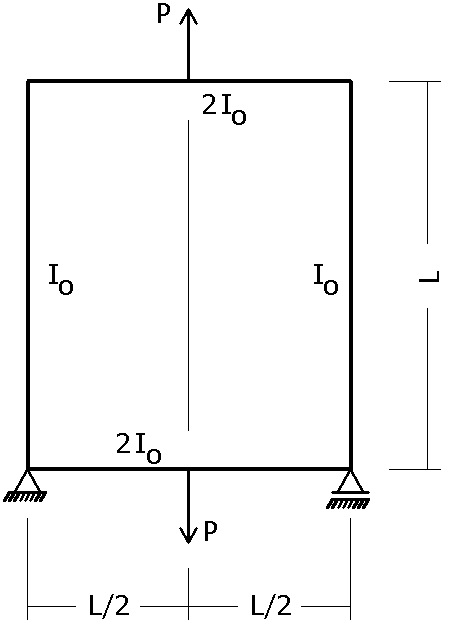
\includegraphics[width=.9\linewidth]{UT4ej2}
\end{center}
\end{minipage}




\ejercicio

Sea la estructura de la figura, conformada por barras de acero (E=210 GPa) de sección tubular de diámetro exterior $\phi =125$ mm y espesor $t=5$ mm. Considerando $P=10$ kN, se pide:



\begin{center}
	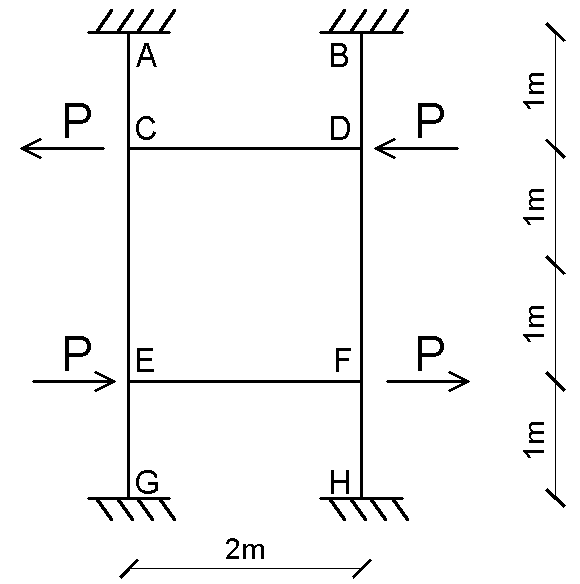
\includegraphics[width=.5\linewidth]{UT4ej3}
\end{center}

\parte Resolver la estructura y trazar diagramas de solicitaciones correspondientes.
\parte Hallar el giro de los puntos C, D, E y F. Bosquejar la deformada de la estructura.

\ejercicio

El pórtico de acero ($E=210$ GPa) mostrado en la figura está construido con perfiles con sección dada por un perfil PNI 24.

\begin{center}
	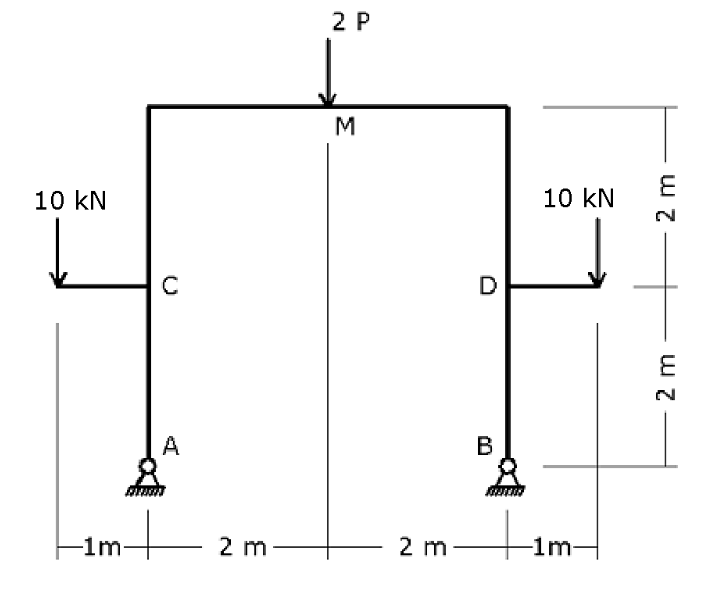
\includegraphics[width=.65\linewidth]{UT4ej4}
\end{center}

\parte Determinar el valor de $P$  para el cual las reacciones en A y B son verticales.
\parte Para ese valor de $P$, calcular el descenso de la sección M y los giros en las secciones C y  D.

\ejercicio

La estructura de acero ($E=210$ GPa) mostrada en la figura recibe la descarga distribuida de un entrepiso sobre el travesaño BC. El marco ABCD consiste en 2 perfiles PNC 20 apareados (][), mientras que el tensor AD se compone de 2 $\phi 16$.

\begin{center}
	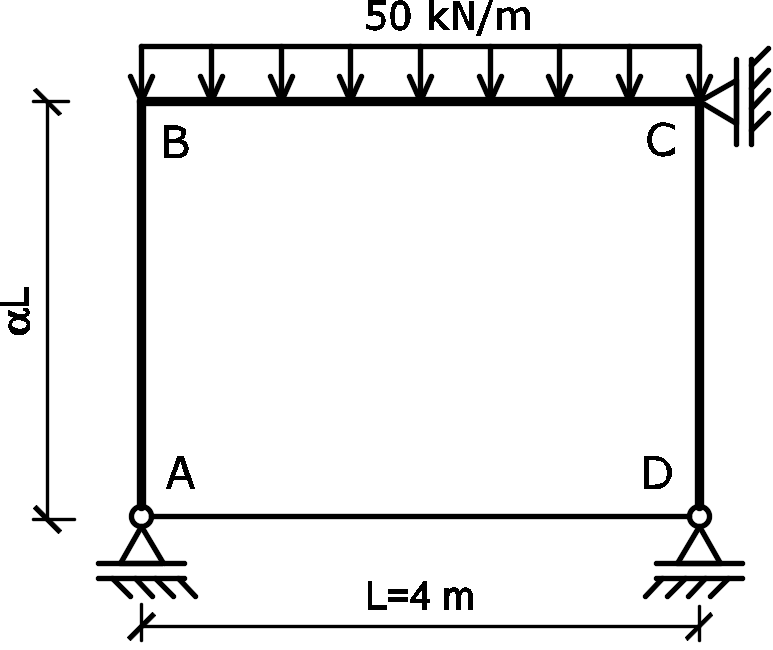
\includegraphics[width=.55\linewidth]{UT4ej5}
\end{center}

Se pide:

\parte Hallar los valores de $\alpha$ para los cuales el máximo momento que tracciona las fibras superiores y el máximo momento que tracciona fibras inferiores en el travesaño BC, son iguales en módulo. 

\parte Para el mayor valor de $\alpha$, trazar los diagramas de solicitaciones.

\ejercicio

Considere la estructura de la Figura \ref{fig61}, con $EI$ uniforme, sometida a las cargas que se indican. Se sabe que $L=2$ m y $H= 100$ kN. %
%

\begin{figure}[htb]
	\centering
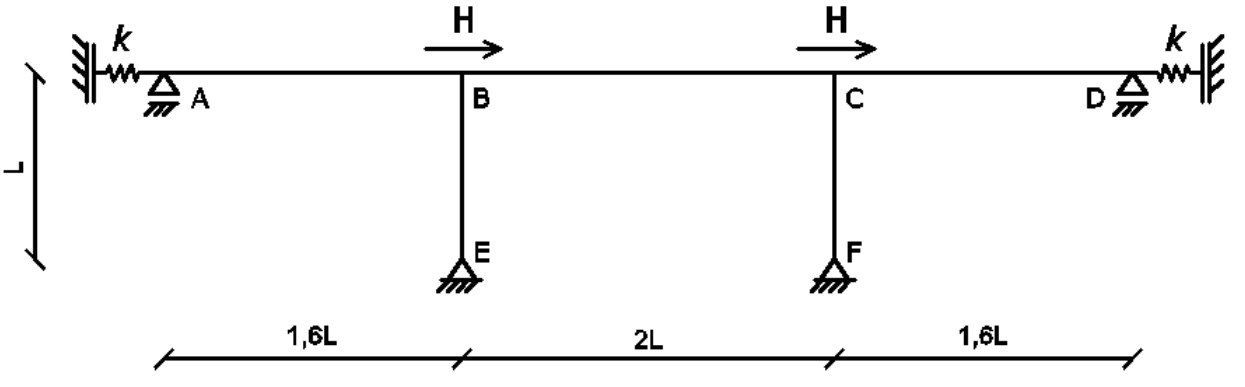
\includegraphics[width=\linewidth]{UT4ej6fig1}
\caption{Esquema de estructura.}
\label{fig61}
\end{figure}

Los pilares (barras BE y CF) están formados por tubulares de acero de diámetro exterior $\phi_{ext} = 45$ cm. %
%
La sección transversal del piso superior (barras AB, BC y CD) es una sección compuesta mostrada en la Figura \ref{fig62}. %
%
Se considera $E_{ACERO} = 210$ GPa y $E_{MADERA} = 10.5$ GPa.

\begin{figure}[htb]
	\centering
	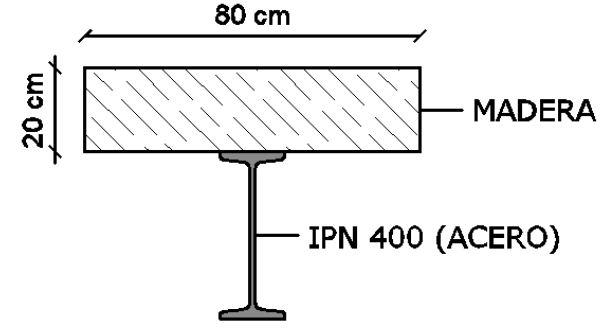
\includegraphics[width=.4\linewidth]{UT4ej6fig2}
	\caption{Esquema de sección transversal de piso superior.}
	\label{fig62}
\end{figure}
%

Se pide:

\parte Determinar el espesor $t$ de los tubulares de forma tal que se cumpla la hipótesis de EI=cte.
\parte Determinar el valor de la constante k de los resortes de forma que el desplazamiento horizontal del piso superior sea $\delta =2.6$ mm hacia la derecha.
\parte Trazar diagramas de solicitaciones y bosquejar la deformada de la estructura.



\ejercicio

La figura muestra una viga atensorada. La viga DAEBF consiste en una escuadría de madera de sección $20 \times 60$ cm, y el tensor ACB en una barra redonda de acero ($E=210$ GPa) de $\phi 16$. %
%
El puntal CE se considera infinitamente rígido. Se considera que $ E_{MADERA} = E_{ACERO} \frac{1}{30}$.

\begin{center}
	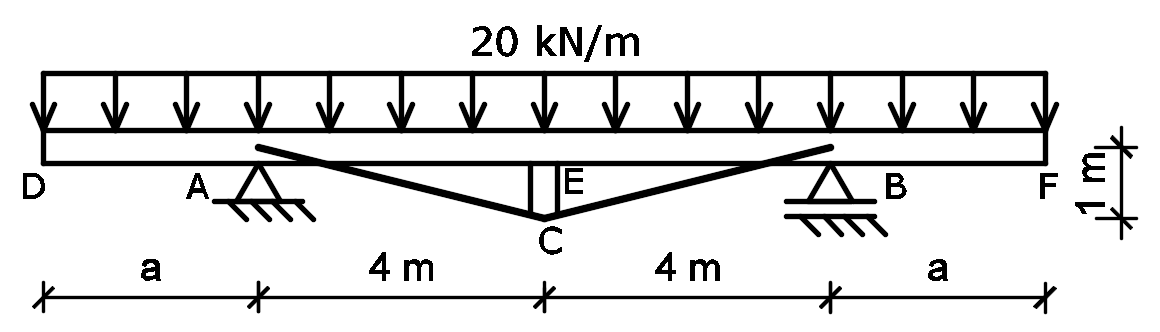
\includegraphics[width=.8\linewidth]{UT4ej7}
\end{center}

\parte Encontrar un resorte vertical en E equivalente al conjunto conformado por el tensor ACB y el puntal CE.
\parte Hallar  a tal que  los tensores estén sometidos a una tensión de $140$ MPa.
\parte Para ese valor de a, calcular la máxima tensión normal en la viga y diagramas de solicitaciones en la estructura.



\ejercicio (adicional) 

La estructura de la figura está compuesta por un marco rígido ABCD de madera ($E=10$ GPa), cuya sección es una escuadría de $15 \times 30$ cm. A su vez existe una barra bi-articulada de acero ($E=210$ GPa) que vincula la barra BC con AD en sus puntos medios, compuesta por 1$\phi$ 20.

\begin{center}
	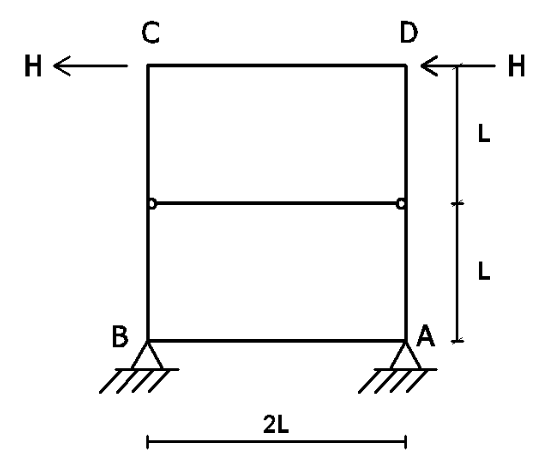
\includegraphics[width=.45\linewidth]{UT4ej8}
\end{center}

Considerando Si $H=8$ kN y $L=2$ m, se pide:

\parte Calcular el desplazamiento del punto C.
\parte Obtener los diagramas de solicitaciones de la estructura.
\parte Bosquejar la deformada de la estructura.

\ejercicio (adicional) 

La estructura de acero de la figura (E=210 GPa) está conformada por perfiles PNI 18. 

\begin{center}
	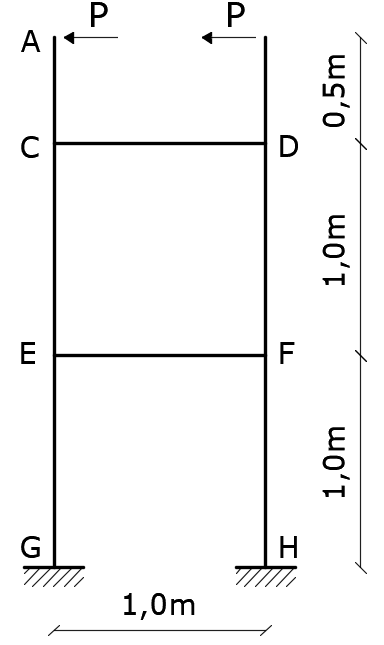
\includegraphics[width=.35\linewidth]{UT4ej9}
\end{center}

\parte Hallar reacciones y diagramas de solicitaciones si $P=15$ kN. 
\parte Bosquejar la deformada de la estructura.

\ejercicio

Sea la viga continua de la figura con $EI$=cte y con vanos de luz $l$.

\begin{center}
	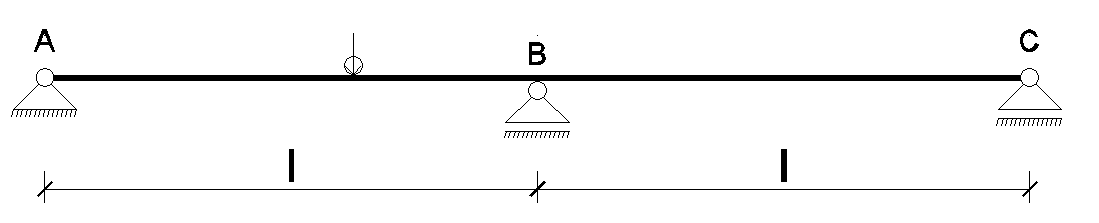
\includegraphics[width=.85\linewidth]{UT4ej10}
\end{center}

\parte Hallar la expresión analítica de la línea de influencia del momento flector $M_B$.



% libroResMat2
% Copyright (C) 2020  J.M. Perez Zerpa, et. al.
%
% This program is free software: you can redistribute it and/or modify
% it under the terms of the GNU General Public License as published by
% the Free Software Foundation version 3 of the License.
%
% This program is distributed in the hope that it will be useful,
% but WITHOUT ANY WARRANTY; without even the implied warranty of
% MERCHANTABILITY or FITNESS FOR A PARTICULAR PURPOSE. See the
% GNU General Public License for more details.
%
% You should have received a copy of the GNU General Public License
% along with this program.  If not, see <http://www.gnu.org/licenses/>.

\chapter{Estructuras tridimensionales de barras}

\section{Emparrillados}

En esta sección se presentan de forma esquemática los conceptos más importantes para la determinación de desplazamientos y solicitaciones en estructuras planas de barras, sometidas a fuerzas perpendiculares al plano de la estructura. %
%
Estas estructuras, tal como fue visto en la Sección~\ref{sec:clasifest}, son llamadas estructuras planoespaciales o emparrillados.

\subsection{Torsión}


En cursos anteriores se abordó la teoría de torsión de Saint-Venant para vigas de sección transversal con doble eje de simetría. %
%
A continuación se enumeran algunas de las magnitudes y conceptos más importantes, aplicando el enfoque utilizado en \citep{Wunderlich2002}.

Sea una barra con un extremo empotrado sometida a un momento torsor $M_t$ se verifica:
%
\begin{equation}
M_t = G J \Theta
\end{equation}
donde $G$ es el módulo de corte, dado por
\begin{equation}
G=\frac{E}{2(1+\nu)},
\end{equation}
$\Theta$ es el barrenado dado por el cociente entre el ángulo de giro del extremo libre y el largo  $\Theta = \theta / \ell$, y $J$ es la inercia torsional de la sección dada por:
%
\begin{equation}
J = \int_{A} \psi_P \dif A.
\end{equation}
%
donde $A$ es el área de la sección transversal y $\psi_P$ es la función de \emph{Prandtl}. %
%
La función de \emph{Prandtl}, puede ser obtenida como la solución del siguiente problema en derivadas parciales:
%
\begin{equation}
\left\{
\begin{array}{lr}
\Delta \psi_P = -2 & \text{en} \, A\\
\psi_P = 0 & \text{sobre } \, \partial A
\end{array}
\right.
\end{equation} 
%

Si se considera un elemento con giros nodales $\theta_1$ y $\theta_2$ se tiene:
%
\begin{equation}
  M_t = G J \frac{\theta_2 - \theta_1}{\ell}
\end{equation}

Por otra parte la energía de deformación torsional está dada por:
%
\begin{equation}
\Pi_{int,\text{torsión}}(\theta_1,\theta_2) = \frac{1}{2} \frac{G J}{\ell} \left( \theta_2 - \theta_1\right)^2.
\end{equation}
%

A partir de la relación entre $\psi_P$ y las tensiones rasantes se puede calcular también el valor de la tensión rasante máxima debida a torsión, dado por:
%
\begin{equation}
\tau_{max} = \frac{M_t}{W_t}
\end{equation}
%
donde $W_t$ es el módulo resistente torsional.


\subsection{Barras sometidas a flexo-torsión}
%
En esta sección se presentan las ecuaciones que relacionan los desplazamientos y fuerzas para barras sometidas a flexión y torsión. %
%
Esto puede ser considerado como una extensión de lo que se vió en la Sección~\ref{sec:mdvig}. %

Se considera un elemento de barra de largo $\ell$ con inercia flexional $I_z$ e inercia torsional $J$. %
%
Las fuerzas nodales consideradas son: por una parte fuerzas y flectores tales que la flexión se produce en el plano formado por los vectores $\bfe_x$ y $\bfe_y$, y por otra parte momentos torsores tales que el vector director (regla de mano derecha) está orientado según el eje $\bfe_x$. %


En general se considera que existe un sistema de coordenadas global  $x,y,z$ y el eje del elemento forma un ángulo $\alpha_y$ con el eje $\bfe_x$ global tal como se muestra en la \autoref{fig:vigators}. %
El ángulo $\alpha_y$ es medido positivo desde el eje $\bfe_x$ global al local con la regla de la mano derecha según el eje $-\bfe_y$.


\begin{figure}[htb]
	\centering
  \def\svgwidth{1\textwidth}
  \input{figs/UT5/viga3d_torsion.pdf_tex}
  \caption{Esquema de elemento de barra a flexo-torsión. Sistemas de coordenadas locales (L) y coordenadas globales representados.}
  \label{fig:vigators}
\end{figure}


En la figura se encuentran representados tanto momentos como giros nodales, donde se considera que los giros y momentos se representan con la misma convención de signo. %
%

Considerando que la barra pertenece al plano $x,z$ se puede descomponer los vectores de momentos y giros en coordenadas locales en una base de coordenadas globales, de la forma:
%
\begin{eqnarray}
M_{x,1,L} &=& \cos(\alpha_y) M_{x,1} + \sin(\alpha_y) M_{z,1} \\
M_{z,1,L} &=& - \sin(\alpha_y) M_{z,1} + \cos(\alpha_y) M_{x,1}
\end{eqnarray}

Considerando también la fuerza según $y$ se tiene:
\begin{eqnarray}
M_{x,1,L} &=& \cos(\alpha_y) M_{x,1} + \sin(\alpha_y) M_{z,1} \\
F_{y,1,L} &=& F_{y,1} \\
M_{z,1,L} &=& - \sin(\alpha_y) M_{z,1} + \cos(\alpha_y) M_{x,1}
\end{eqnarray}

De forma equivalente para los desplazamientos y giros se tiene:
\begin{eqnarray}
\theta_{x,1,L} &=& \cos(\alpha_y) \theta_{x,1} + \sin(\alpha_y) \theta_{z,1} \\
v_{y,1,L} &=& v_{y,1} \\
\theta_{z,1,L} &=& - \sin(\alpha_y) \theta_{z,1} + \cos(\alpha_y) \theta_{x,1}
\end{eqnarray}
%
y expresiones equivalentes para el nodo 2.

Definiendo el vector de desplazamientos nodales en coordenadas globales:
\begin{equation}
\bfu = 
\left[
\begin{matrix}
\theta_{x,1} & v_{y,1} & \theta_{z,1} & \theta_{x,2} & v_{y,2} & \theta_{z,2}
\end{matrix}
\right]^T
\end{equation}
%
y el vector de desplazamientos nodales en coordenadas locales:
\begin{equation}
\bfu_L = 
\left[
\begin{matrix}
\theta_{x,1,L} & v_{y,1,L} & \theta_{z,1,L} & \theta_{x,2,L} & v_{y,2,L} & \theta_{z,2,L}
\end{matrix}
\right]^T
\end{equation}
%
se puede representar la relación entre desplazamientos en diferentes sistemas de coordenadas como:
%
\begin{equation}\label{eqn:matrot}
\bfu = \bfR \bfu_L
\end{equation}
donde
\begin{equation}
\bfR = 
\left[
\begin{matrix}
\cos(\alpha_y) & 0  & -\sin(\alpha_y) & 0 & 0 & 0\\
 0 & 1 & 0 &  0 & 0 & 0\\
\sin(\alpha_y) & 0  & \cos(\alpha_y) & 0 & 0 & 0\\
%
0 & 0 & 0 & \cos(\alpha_y) & 0  & -\sin(\alpha_y) \\
0 & 0 & 0 & 0 & 1 & 0 \\
0 & 0 & 0 & \sin(\alpha_y) & 0  & \cos(\alpha_y)
\end{matrix}
\right].
%
\end{equation}


Esta matriz de rotación puede ser obtenida también aplicando los conceptos de algebra lineal de matriz de cambio de base.

La energía potencial de deformación total está dada por la suma de las energías potenciales debidas a torsión y flexión, las cuales pueden ser representadas en coordenadas locales como:
%
\begin{equation}
\Pi_{int} (\bfu_L ) = \Pi_{int,\text{torsión}}(\theta_{x,1,L},\theta_{x,2,L}) + \Pi_{int,\text{flexión}}(v_{y,1,L}, \theta_{z,1,L},v_{y,2,L},\theta_{z,2,L})
\end{equation}
%
donde $\Pi_{int,\text{flexión}}$ está dada por la Ecuación~\eqref{eqn:Uflex}. %
%
La energía potencial de las fuerzas externas está dada por $\Pi_{ext} (\bfu_L) = -\bfu_L^T \bff_L$ donde $\bff_L$ está dado por:
\begin{equation}
\bff_L = 
\left[
\begin{matrix}
	M_{x,1,L} & F_{y,1,L} & M_{z,1,L} & M_{x,2,L} & F_{y,2,L} & M_{z,2,L}
\end{matrix}
\right]^T.
\end{equation}


Utilizando el principio de mínima energía potencial total y aplicando las condiciones del primer teorema de Castigliano se tienen las siguientes cuatro condiciones para flexión:
\begin{eqnarray}
\frac{\partial \Pi_{int,\text{flexión}}}{\partial v_{y,1,L}} =  F_{y,1,L}  \qquad \frac{\partial \Pi_{int,\text{flexión}}}{\partial \theta_{z,1,L}} =  M_{z,1,L} \\
\frac{\partial \Pi_{int,\text{flexión}}}{\partial v_{y,2,L}} =  F_{y,2,L} \qquad \frac{\partial \Pi_{int,\text{flexión}}}{\partial \theta_{z,2,L}} =  M_{z,2,L}
\end{eqnarray}
y las siguientes condiciones para torsión:
%
\begin{equation}
\frac{\partial \Pi_{int,\text{torsión}}}{\partial \theta_{x,1,L}} =  M_{x,1,L} \qquad 
\frac{\partial \Pi_{int,\text{torsión}}}{\partial \theta_{x,2,L}} =  M_{x,2,L}
\end{equation}

Sustituyendo las expresiones de las energías de deformación se obtiene que las condiciones de Castigliano son equivalentes al sistema de ecuaciones:
\begin{equation}
\bfK_L \bfu_L = \bff_L
\end{equation}
%
donde la matriz $\bfK_L$ es la matriz de rigidez en coordenadas locales, dada por:
%
\begin{equation}\label{eqn:matrigtf}
	\bfK_L = \left[
	\begin{matrix}
		\dfrac{GJ}{\ell} & 0 & 0 & - \dfrac{GJ}{\ell} & 0 & 0 \\[3mm]
		%
		0 &  12 \dfrac{EI_z}{\ell^{3}} & 6 \dfrac{EI_z}{\ell^{2}} &  0& -12 \dfrac{EI_z}{\ell^{3}} & 6 \dfrac{EI_z}{\ell^{2}} \\[3mm]
		0 &  6 \dfrac{EI_z}{\ell^{2}} & 4 \dfrac{EI_z}{\ell} & 0& -6 \dfrac{EI_z}{\ell^{2}} & 2 \dfrac{EI_z}{\ell} \\[3mm]
		-\dfrac{GJ}{\ell} & 0 & 0 &  \dfrac{GJ}{\ell} & 0 & 0 \\[3mm]
		%
		0 &  -12 \dfrac{EI_z}{\ell^{3}} & -6 \dfrac{EI_z}{\ell^{2}} &0&  12 \dfrac{EI_z}{\ell^{3}} & -6 \dfrac{EI_z}{\ell^{2}} \\[3mm]
		0 &  6 \dfrac{EI_z}{\ell^{2}} & 2 \dfrac{EI_z}{\ell} & 0 & -6 \dfrac{EI_z}{\ell^{2}} & 4 \dfrac{EI_z}{\ell} \\[3mm]
	\end{matrix}
	\right].
\end{equation}

Utilizando que $\bfu_L = \bfR^T \bfu$  y que  $\bff_L = \bfR^T \bff$  se obtiene el sistema en coordenadas globales:

\begin{equation}
\bfK \bfu = \bff
\end{equation}

donde la matriz de rigidez $\bfK$ es la matriz de rigidez en coordenadas globales dada por
\begin{equation}\label{eqn:matrigtfglo}
\bfK = \bfR \bfK_L \bfR^T.
\end{equation}

Para un emparrillado formado por $n$ elementos de barra se debe calcular cada matriz en coordenadas globales y realizar el ensamblado de forma similar a como es realizado para elementos de reticulados o pórticos. %
%

\subsection{Ejemplo}

Sea la estructura mostrada en la Figura~\ref{fig:UT5_ejemplo}, donde todas las barras tienen inercia flexional $I$ e inercia torsional $J$ a determinar y están formadas por un material de módulo de Young $E$. %
Se considera que $E=210$ GPa, $\nu=0.3$, $\ell=2 $ m, la sección transversal es cuadrada de lado $5$ cm. %
%
Se desea calcular los desplazamientos nodales para una carga puntual $P=4 $ kN.

\begin{figure}[htb]
	\centering
	\def\svgwidth{0.6\textwidth}
	\input{figs/UT5/UT5_ejemplo.pdf_tex}
	\caption{Esquema básico de cálculo de ejemplo de emparrillado.}
	\label{fig:UT5_ejemplo}
\end{figure}

La barra con la carga puntual aplicada tiene una geometría y condiciones de vínculo simétricos por lo que el giro $\theta_x$ debe ser nulo.
%
Considerando está condición de simetría  y dividiendo la estructura en dos mitades, se obtiene el esquema básico simplificado que se muestra en la Figura~\ref{fig:UT5_ejemplo2}.

\begin{figure}[htb]
	\centering
	\def\svgwidth{0.7\textwidth}
	\input{figs/UT5/UT5_ejemplo_connodos.pdf_tex}
	\caption{Esquema de mitad de estructura de ejemplo de emparrillado.}
	\label{fig:UT5_ejemplo2}
\end{figure}

Utilizando la numeración definida, se establece la conectividad de los elementos como Elemento 1: del nodo 1 al 2 y Elemento 2: del nodos 2 al 3. %
Los sistemas de coordenadas locales considerados se muestran en la figura.

Para el cálculo de las matrices de rigidez cada elemento se usa la expresión de la Ecuación~\eqref{eqn:matrigtfglo}.

Para el elemento 1, $\bfK_L$ está dada por la expresión de la ecuación~\eqref{eqn:matrigtf} y $\bfR$ es la matriz identidad de tamaño $6\times6$.

Para el elemento 2, $\bfK_L$ es calculada considerando el largo $\ell/2$ en la ecuación~\eqref{eqn:matrigtf} y para la matriz de rotación se considera $\alpha_y=-\pi/2$ en la ecuación \eqref{eqn:matrot} por lo tanto
\begin{equation}
\bfR = 
\left[
\begin{matrix}
0 & 0  & 1 & 0 & 0 & 0\\
0 & 1 & 0 &  0 & 0 & 0\\
-1 & 0  & 0 & 0 & 0 & 0\\
%
0 & 0 & 0 & 0 & 0  & 1 \\
0 & 0 & 0 & 0 & 1 & 0 \\
0 & 0 & 0 & -1 & 0  & 0
\end{matrix}
\right].
%
\end{equation}


El módulo de corte es $G=\frac{E}{2(1+\nu)} = 80.7 $ GPa. La inercia flexional es $I= 5.208 \times 10^{-7}$ m$^4$ y la inercia torsional, para una sección cuadrada, está dada por $J= 0.141 (0.05)^4 = 8.81 \times 10^{-7}$ m$^4$.

Los desplazamientos generalizados para el nodo 2 son:
%
$$
\theta_{x,2} = -0.006898
\quad 
v_2 = -0.04876
\quad
\theta_{z,2} = -0.03657
$$
%
y para el nodo 3 son:
$$
v_3 = -0.05374
\quad
\theta_{z,3} = 
-0.036571
$$


\subsection{Implementación computacional}

En el Código~\ref{cod:emparrillados} en la Sección~\ref{sec:codut5} se presenta una implementación en GNU-Octave del método descrito y su aplicación para la resolución del ejemplo visto. %
%
El código ha recibido aportes y modificaciones de estudiantes del curso 2019, los nombres de los autores fueron agregados al código y los cambios están visibles en el repositorio del código fuente de este documento.

Para validar los resultados obtenidos con el Código~\ref{cod:emparrillados} se realiza otro modelo usando la herramienta ONSAS. Se realiza un primer modelo con análisis lineal y la misma geometría, luego otro modelo con la geometría completa y finalmente un modelo con la geometría completa y análisis no lineal para una carga máxima 20 veces superior a $P$. El archivo del modelo está disponible en el repositorio de ONSAS\footnote{\href{https://github.com/ONSAS/ONSAS/blob/master/examples/onsasExample_emparrillado.m}{github.com/ONSAS/ONSAS/blob/master/examples/onsasExample\_emparrillado.m}} La figura deformada para el estado de cargas máximo con el análisis no lineal es mostrado en la Figura~\ref{fig:empa}.

\begin{figure}[htb]
	\centering
	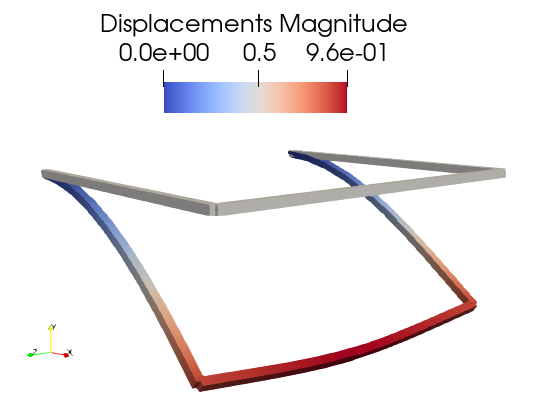
\includegraphics[width=0.65\textwidth]{defONSASemparrillado}
	\caption{Deformada emparrillado, con análisis no lineal y estado de carga 20 $P$ (factor de esacala: 1).}
	\label{fig:empa}
\end{figure}


\subsection{Cargas equivalentes nodales}

Para el análisis de la estructura tridimensional completa mostrada en la Figura~\ref{fig:UT5_ejemplo} utilizando un método analítico, es posible llevar la carga en el punto medio a los nodos, utilizando el enfoque de cargas equivalentes presentado en la Sección~\ref{sec:cargequiv}.


\section{Estructuras tridimensionales de barras}

En el caso de estructuras tridimensionales, los elementos de barra pueden estar sometidos a esfuerzos de fuerzas y momentos que producen 6 solicitaciones internas: directa, torsión, 2 flectores y 2 cortantes (correspondientes a la flexión en los dos planos definidos por los ejes de coordenadas locales transversales).

\subsection{Elemento de viga sometido a flexo compresión esviada}

El caso de flexión esviada corresponde a vigas sometidas a momentos flectores con componentes no nulas en los dos ejes de coordenadas locales transversales (siendo estos los ejes de los momentos de inercial principales). %

El desarrollo de las ecuaciones para vigas sometidas a esfuerzos axiales y transversales es equivalente al presentado en la Sección~\ref{sec:teoviga}, considerando que los giros de las secciones son no nulos tanto en el eje $y$ como el eje $z$, esto es $\theta_z \neq 0$ y $\theta_y \neq 0$. %
%
Al mismo tiempo se tiene que ambos desplazamientos transversales $v$ y $w$ son no nulos.

También se mantiene la hipótesis de que caras planas permanecen planas, por lo que el desplazamiento de un punto ubicado en un punto con coordenadas $x,y,z$ puede ser escrito como:
%
\begin{equation} \label{eqn:despaxidosdir}
  u(x,y,z) = u_G(x) - y \theta_z(x) + z \theta_y(x).
\end{equation}

Realizando un desarrollo equivalente al del caso plano se puede obtener las relaciones 
%
\begin{equation}
 \theta_z(x) = \frac{\partial v}{\partial x}(x), \qquad  \theta_y(x) = - \frac{\partial w}{\partial x}(x),
\end{equation}
%
y la expresión de la tensión axial:
%
\begin{equation}\label{eqn:tensaxiflexesv}
\boxed{
	\sigma(x,y,z) = \frac{	N (x) }{A}
	- y \frac{	M_z (x) }{I_z} + z \frac{	M_y (x) }{I_y} 
}
\end{equation}

En clase se presentará el razonamiento utilizado en este desarrollo así como también se verán ejemplos prácticos.




\subsection{Elemento de pórtico tridimensional}

En clase se presentará brevemente el elemento de barra tridimensional, el cual es considerado sometido a torsión, flexión en ambos planos (es decir \textit{flexión esviada}) y directa. %
%
En este curso se realizar un especial énfasis en el análisis de estructuras de pórtico 3D isostáticas.

\section{Ejercicios}
\setcounter{ejercicio}{0}

\ejercicio

Sea la estructura mostrada en la figura, construida con caños de acero ($E=210$ GPa y $\nu =0.3$) de $\phi_{ext} = 100$ mm y $t=8$ mm.

\begin{center}
	\def\svgwidth{0.5\textwidth}
	\input{./figs/UT5/UT5_ej1.pdf_tex}
\end{center}

Considerando $P=4$ kN y $L=1.0$ m, se pide:
%
\parte Calcular los desplazamientos y giros nodales y trazar diagramas de solicitaciones usando:
\begin{enumerate}
\item Equilibrios y valores de deflexiones y giros en ménsulas. 
\item Análisis matricial.
\end{enumerate}
\parte Comparar los resultados hallados en a) con los obtenidos mediante:
  \begin{enumerate}
   \item una versión modificada del código \ref{cod:emparrillados}
  \item alguna de las herramientas computacionales presentadas en el curso
  \end{enumerate}


\ejercicio

Se construye un emparrillado con caños de acero (E=210 GPa, $\nu=0.3$) de $\phi_{ext}=100$ mm y $t=8$ mm, sometido a dos estados de carga mostrados en las figuras.

\begin{center}
	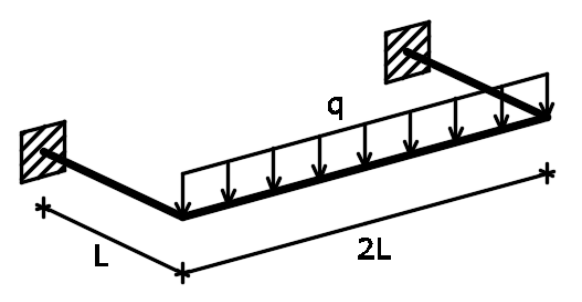
\includegraphics[width=0.4\linewidth]{UT5ej2a}
	\hspace{0.1\linewidth}
	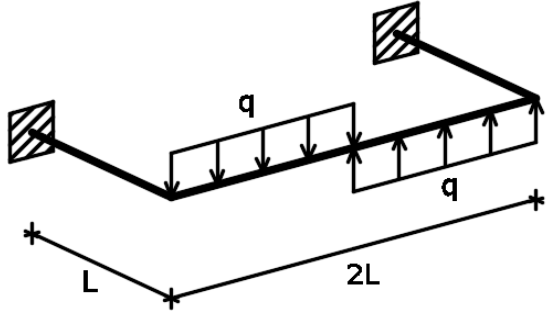
\includegraphics[width=0.4\linewidth]{UT5ej2b}
\end{center}

Considerando $q=2$ kN/m y $L=1$ m, se pide:

\parte Resolver mediante el método de análisis matricial, considerando la simetría o antisimetría del problema para trabajar con una cantidad de barras reducida.
%
\parte Trazar diagramas de solicitaciones y comparar con los obtenidos con un modelo computacional de la estructura.

\vspace{1cm}
El emparrillado analizado es ahora usado como parte de la estructura de una hamaca con su respectivo esquema básico de cálculo como se muestra en las figuras. %
Las cargas $q$ consideradas en las partes anteriores se aplican únicamente en la barra EF.

\begin{center}
	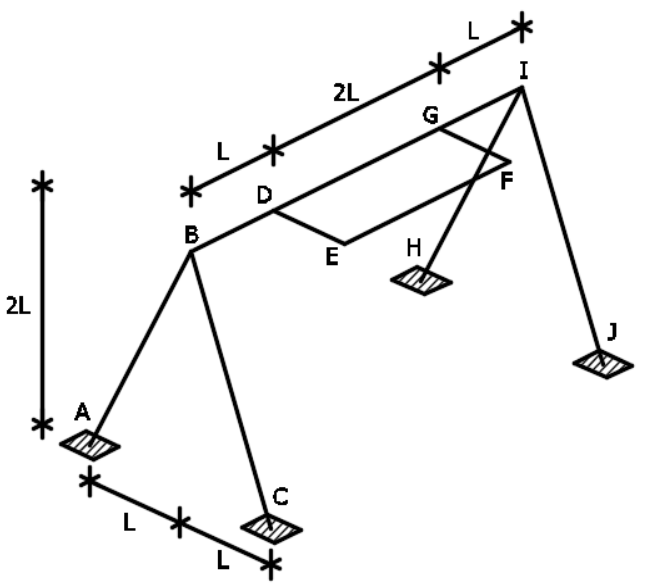
\includegraphics[width=0.5\linewidth]{UT5ej2c}
	\hspace{0.05\linewidth}
	\includegraphics[width=0.4\linewidth]{UT5ej2d}
\end{center}

Considerando que todas las barras están compuestas por el mismo tubular que el emparrillado, se pide:
%
\parte Modelar la estructura con un programa computacional y comparar los resultados con los obtenidos en las partes anteriores en la zona del emparrillado. 


\ejercicio

Sea un emparrillado modificado con respecto al del Ejercicio 2, en el cual se agrega una barra adicional, que está sometida a una carga $q=2$ kN/m, como se muestra en la figura.

\begin{center}
	\includegraphics[width=0.6\linewidth]{UT5ej3}
\end{center}

Se pide:
\parte Resolver mediante análisis matricial. Trazar diagramas de solicitaciones.
\parte Comparar resultados obtenidos en a) con los obtenidos utilizando alguna herramienta computacional.


\ejercicio

Sea la estructura mostrada en la figura, construida con barras de acero (E=210 GPa, $\nu=0.3$) de sección circular maciza de diámetro $\phi_{ext}=105$ mm. 

\begin{center}
	\includegraphics[width=0.6\linewidth]{UT5ej4}
\end{center}

Considerando P=4 kN y L=3.0 m, se pide:

\parte Modificar el código presentado en clase para resolución de emparrillados y obtener desplazamientos y giros nodales. Con los resultados obtenidos trazar diagramas de solicitaciones.
\parte Utilizar algún programa computacional para resolver el problema y verificar los resultados.
\parte Repetir b) descomponiendo en una estructura simétrica y otra antisimétrica.




\ejercicio

La estructura tridimensional de hormigón ($E=30$ GPa y $\nu=0.2$) mostrada en las está conformada por pilares de sección cuadrada $30 \times 30$ cm y vigas de $b=20$ cm y  $h=50$ cm.

\begin{center}
	\includegraphics[width=0.45\linewidth]{UT5ej5a}
	\hspace{0.05\linewidth}
	\includegraphics[width=0.45\linewidth]{UT5ej5b}
\end{center}

Para el caso de la estructura a la izquierda se considera $P=20$ kN y se pide:
%
\parte Estudiar los pórticos planos ABCD y EFGH independientes del resto de la estructura en forma analítica. 
%
\parte Modelar la estructura completa en un programa computacional y comparar  los resultados con los hallados en a). %
%
Para el caso de la estructura a la derecha se considera $q=10$ kN/m sobre la viga AB y se pide:
%
\parte Indicar qué modelo plano realizaría para estudiar el pórtico ABCD considerando que los puntos E y F están fijos. Obtener computacionalmente resultados de ese modelo. 
%
\parte Analizar los resultados de modelar la estructura tridimensional y comparar con los obtenidos en c). 

\ejercicio

Se desea estudiar un aerogenerador cuyas dimensiones se muestran en la figura a la izquierda. Todas las palas (o aspas) tienen el mismo largo y tienen mismo ángulo de apertura 120$^\circ$. %
%
%
En la figura a la derecha se muestra un estado de cargas estáticas idealizado, de interés para el diseño. %
%
Las fuerzas actuantes son:
\begin{itemize}
\item Una fuerza puntual de 80 kN sobre cada punto: F, G y H, representando la fuerza del viento sobre las aspas. 
\item Una fuerza del viento sobre la torre que se ha simplificado como una fuerza en B horizontal de 20 kN. 
\item El peso de las aspas de 30 kN que se aplica como una carga puntual en el punto E.
\item La carga distribuida de 6.5 kN/m que representa el peso de la turbina.
\end{itemize}

Se pide: calcular las reacciones en A y los diagramas de solicitaciones.

\begin{center}
	\def\svgwidth{0.5\textwidth}
\input{figs/UT5/ej56.pdf_tex}
\end{center}

\ejercicio

Se desea analizar la estructura de un pasamanos considerando un correspondiente Esquema Básico de Cálculo como se muestra en las figuras.

\begin{center}
	\includegraphics[width=0.85\linewidth]{UT5ej7}
\end{center}

La estructura está compuesta por tubulares de acero ($E=210$ GPa y $\nu=0.3$) de $\phi_{ext}=80$ mm y $t=6$ mm. %
%
Sobre las barras transversales actúa una carga q=3 kN/m y L=1.0 m. Se pide:

\parte Considerar que las barras no presentan rigidez a torsión y calcular analíticamente las solicitaciones en cada una de las barras.
\parte Considerar la rigidez a torsión en las barras y obtener resultados de modelar computacionalmente la estructura.
\parte Comparar resultados obtenidos en a) y b).


\ejercicio (adicional) 

El emparrillado de la figura simula el entrepiso con vigas de una edificación. 

\begin{center}
	\includegraphics[width=0.65\linewidth]{UT5ej8}
\end{center}

Considerar que todas las vigas son de hormigón (E=30 GPa, $\nu=0.2$) y su sección es 30x80 cm. Las mismas están cargadas con una carga q=15 kN/m y L=5.0 m.

\parte Modelar la estructura computacionalmente. Analizar el comportamiento de las solicitaciones y la deformada.
\parte Si se desprecia la rigidez a torsión de las vigas, ¿cómo se ven afectadas las solicitaciones y deformaciones de las vigas? Analizar.


\ejercicio (adicional) 

La estructura planoespacial mostrada en la figura está formada por barras de misma sección y longitud que el emparrillado del Ejercicio 2.

\begin{center}
	\includegraphics[width=0.75\linewidth]{UT5ej9}
\end{center}

Se pide: trazar diagramas de solicitaciones para $P=10$ kN.


% libroResMat2
% Copyright (C) 2020  J.M. Perez Zerpa, et. al.
%
% This program is free software: you can redistribute it and/or modify
% it under the terms of the GNU General Public License as published by
% the Free Software Foundation version 3 of the License.
%
% This program is distributed in the hope that it will be useful,
% but WITHOUT ANY WARRANTY; without even the implied warranty of
% MERCHANTABILITY or FITNESS FOR A PARTICULAR PURPOSE. See the
% GNU General Public License for more details.
%
% You should have received a copy of the GNU General Public License
% along with this program.  If not, see <http://www.gnu.org/licenses/>.

\chapter{Análisis Seccional}

En esta unidad se presentan conceptos vinculados al análisis de tensiones en secciones transversales en vigas y/o columnas. %

En la Sección~\ref{sec:lnnc} se desarrolla y aplica un método práctico para el cálculo del Núcleo Central en secciones de cualquier forma. %
%
Parte del desarrollo es similar al usado en \citep{massood2001} mientras que otra parte fue desarrollada por los autores. %
%
Un desarrollo anterior se puede encontrar en el capítulo VIII de \citep{Timoshenko1953}. %
%
En la Sección~\ref{sec:nucleocentral} se presenta el análisis seccional para materiales que no soportan tracción, basado principalmente en el apartado 52 de \citep{Timoshenko1953} con una notación similar a la utilizada en los materiales de \textit{Resistencia de Materiales IIn} elaborados principalmente por el Prof. Atilio Morquio.

% -----------------------------------------------
% -----------------------------------------------
\section{Análisis Lineal de Secciones} \label{sec:lnnc}

En esta sección se presentan dos conceptos básicos en el análisis lineal de tensiones en secciones de elementos de viga: Línea Neutra (presentado en la Sección~\ref{sec:lineaneutra}) y Núcleo Central (presentado en la Sección~\ref{sec:nucleocentral}).

\subsection{Línea neutra} \label{sec:lineaneutra}

Se presenta a continuación una definición conceptual de Línea Neutra (LN).

\cajaconcepto{Definición: Línea Neutra}
{Sea una sección transversal de una viga sometida a esfuerzos de flexión, se define la \textbf{Línea Neutra} como el conjunto de puntos con \textbf{tensión axial nula}.}

La definición en términos de la función tensión puede ser enunciada como, que dada una sección transversal ubicada en un punto de coordenada $x$, la Línea Neutra es el conjunto de puntos $(y,z)$ que verifican: $\sigma(x,y,z) = 0$.

Existe una correspondencia biunívoca entre cada línea neutra y un punto de aplicación de la carga. %
%
A continuación se muestran los desarrollos para obtener la LN a partir del punto de aplicación y luego el desarrollo inverso.

\subsubsection{Determinación de la Línea Neutra a partir del punto de aplicación}


Se considera una viga con un corte en una sección tranversal en la posición $x$, y una carga $N$ aplicada en un punto de coordenadas $(y_A,z_A)$ como se muestra en la \autoref{fig:NCesquema1}. %

\begin{figure}[htb]
	\centering
   \def\svgwidth{0.9\textwidth}
   \input{figs/UT6/NCesquema1.pdf_tex}
	\caption{Esquema de sección, sistema de coordenadas considerado y equivalencia de torsores de carga y solicitaciones internas.}
	\label{fig:NCesquema1}
\end{figure}

Esta carga puede estar asociada tanto a cargas externas como a cargas internas producidas por el resto del elemento de viga. %
%
Se calcula el torsor equivalente en el baricentro de la sección, esto es, fuerza y momentos equivalentes:
%
\begin{equation}
N(x) = N, \qquad  M_z(x) = -N y_A \quad  \text{y} \quad M_y(x) = N z_A.
\end{equation}
%
Estas tres solicitaciones representan las solicitaciones internas correspondientes.


Sustituyendo las expresiones de las solicitaciones en la Ecuación~\eqref{eqn:tensaxiflexesv} y desarrollando se obtiene:
%
\begin{equation}
\sigma(x,y,z) = \frac{N(x)}{A}
\left(1 +  \frac{ y_A}{\rho_z^2} y +  \frac{ z_A}{\rho_y^2} z \right),
\end{equation}
%
donde fueron introducidas dos propiedades geométricas, llamadas radio de giro: $\rho_y = \sqrt{ I_y / A}$ y $\rho_z = \sqrt{ I_z / A}$. %
%

La condición de pertenencia a la LN es equivalente a anular la expresión de tensión axial. %
%
Por lo tanto, dado un punto de aplicación $(y_A,z_A)$, se demuestra que la ecuación de la LN es:
%
\begin{equation}\label{eqn:AptoLN}
\boxed{1 +  \frac{ y_A}{\rho_z^2} y +  \frac{ z_A}{\rho_y^2} z = 0}
\end{equation}

Se observa que la recta está contenida en el $plano$ $yz$ y no pasa por el origen, esto se debe a la existencia de una fuerza de directa aplicada.
%


\subsubsection{Determinación de punto de aplicación a partir de la Línea Neutra}

En esta sección se considera el caso en el cual se tiene una LN y se desea encontrar el punto de aplicación de la carga. %
%
Dada la ecuación de una recta genérica que no pasa por el origen:
$$
a y + b z +  c = 0,
$$
%
y usando que $(c\neq0)$ se obtiene la expresión:
%
\begin{equation}\label{eqn:ecrecta}
\frac{a}{c} y + \frac{b}{c} z +  1 = 0.
\end{equation}

Igualando los coeficientes de los polinomios de las expresión de las Ecuaciones \eqref{eqn:AptoLN} y \eqref{eqn:ecrecta} se tiene:
%
\begin{equation}
\boxed{y_A = \frac{a}{c} \rho_z^2
\qquad
z_A = \frac{b}{c} \rho_y^2}
\end{equation}

Dado que hay directa aplicada la recta que define la LN no pasa por el origen, por lo tanto se cumple que $c\neq0$.




% -------------------------------
\subsection{Núcleo central} \label{sec:nucleocentral}

Considerando una sección transversal cualquiera, se presenta una definición conceptual de Núcleo Central.

\cajaconcepto{Definición: Núcleo central}
{Se denomina Núcleo Central (NC) al lugar geométrico de los puntos del plano de la sección en los cuales una fuerza puntual de tracción (o compresión) aplicada generaría que toda la sección sea traccionada (o comprimida).}

Esto es equivalente a decir que, para cualquier punto de aplicación perteneciente al NC, la línea neutra correspondiente no corta a la sección.


\subsubsection{Cálculo de NC para secciones con borde suave}

El enfoque utilizado para el cálculo del NC es similar al utilizado en \citep{massood2001}. %
%

Se considera que el contorno de la sección transversal está dado por una curva paramétrica \textit{regular} y \textit{suave}. %
%
\begin{equation}
\mcC %
\left\{
\begin{array}{l}
y = y(t) \\
z = z(t) 
\end{array}
\right.
\end{equation}
donde las coordenadas $y$ y $z$ están medidas en el sistema de coordenadas locales.

La condición de regularidad implica que para todo parámetro $t$ se tiene que o bien $\dot{z}(t)\neq 0$ o $\dot{y}(t)\neq 0$, pero en ningún caso se cumple que $\dot{y}(t) = \dot{z}(t) = 0$. %
%
La condición de suavidad implica que tanto  $y(t)$ como $z(t)$ con funciones con derivada primera continua, es decir: de tipo $C^1$.

En la \autoref{fig:NCesquema2} se muestra un esquema de la sección transversal. %
%
En cada punto del contorno se puede definir una LN tangente, la cual se corresponderá con un punto de aplicación.

\begin{figure}[htb]
	\centering
	\includegraphics[width=0.5\textwidth]{NCesquema2}
	\caption{Esquema de sección y sistema de coordenadas considerado.}
	\label{fig:NCesquema2}
\end{figure}

Se desea obtener la curva paramétrica de los puntos de aplicación $(y_A(t),z_A(t))$, asociadas a las líneas neutras tangentes a la sección transversal en cada punto $y(t),z(t)$ y que no cortan a la sección. Por lo tanto, para dichos puntos de aplicación, existe al menos un punto del contorno de la sección correspondiente a la LN en que $\sigma(x,y(t),z(t)) = 0$. Utilizando la expresión de la Ecuación~\eqref{eqn:AptoLN} se tiene:
%
\begin{equation}
1 +  \frac{ y_A(t)}{\rho_z^2} y(t) +  \frac{ z_A(t)}{\rho_y^2} z(t) = 0
\end{equation}

Se ha encontrado entonces un punto de aplicación $(y_A(t),z_A(t))$ en el que la expresión de la tensión axial para los distintos puntos del contorno es,
\begin{equation}\label{eqn:NC1}
\sigma(x,y(\hat t),z(\hat t)) = \frac{N}{A} \left(1 +  \frac{ y_A(t)}{\rho_z^2} y(\hat t) +  \frac{ z_A(t)}{\rho_y^2} z(\hat t) \right)= 0
\end{equation}
Donde $\hat t$ es la variable que permite recorrer el contorno de la sección.



Los puntos del contorno de la sección, pertenecientes a la LN tangente a la sección y que no cortan a la misma, donde $\sigma(x,y(\hat t),z(\hat t)) = 0$, cumplen además que son puntos críticos, mínimo si $N(x)>0$ y máximo si $N(x)<0$. Imponiendo esta condición se obtiene:

\begin{equation}\label{eqn:NC2}
\frac{\partial \sigma}{\partial \hat t}(x,y(\hat t=t),z(\hat t=t)) = 0 = \frac{ y_A(t)}{\rho_z^2} \dot{y}(t) +  \frac{ z_A(t)}{\rho_y^2} \dot{z}(t)
\end{equation}

Combinando la Ecuación~\eqref{eqn:NC1} con la Ecuación~\eqref{eqn:NC2} y usando que $\mcC$ es regular y no pasa por el origen, se obtiene la curva paramétrica del borde del núcleo central:
%
\begin{eqnarray}
y_A(t) &=& - \frac{ \dot{z}(t) }{ \dot{z}(t) y(t) - \dot{y}(t) z(t) } \rho^2_z \label{eqn:ecsPSy} \\
z_A(t) &=& \frac{ \dot{y}(t) }{ \dot{z}(t) y(t) - \dot{y}(t) z(t) } \rho^2_y \label{eqn:ecsPSz}
\end{eqnarray}

\subsubsection{Cálculo de NC para secciones con borde no suave}

En la \autoref{fig:NCesquema3} se muestra el esquema, en el $plano$ $yz$, de una sección con borde no suave para la cual, en el punto $R$ existe una discontinuidad en el vector tangente al borde. %
%
Esto provoca que las Ecuaciones \eqref{eqn:ecsPSy} y \eqref{eqn:ecsPSz} pierdan su validez.

\begin{figure}[htb]
	\centering
	\includegraphics[width=0.5\textwidth]{NCesquema3}
	\caption{Esquema de sección en el plano.}
	\label{fig:NCesquema3}
\end{figure}

Se conoce que los puntos de aplicación $(y_1,z_1)$ y $(y_2,z_2)$ pertenecen al NC y tienen asociados las líneas neutras $LN_1$ y $LN_2$ respectivamente. La unión de los puntos de aplicación de las fuerzas de directa $N_1$ y $N_2$ forman una recta $r$, que se puede expresar como:
%
$$
r: z-z_1 = \frac{(z_1-z_2)}{(y_1-y_2)}(y-y_1).
$$

Desarrollando, factorizando y normalizando el término independiente, se obtiene:
%
\begin{equation}
\frac{y(z_1-z_2)-z(y_1-y_2)}{z_1y_2-y_1z_2}=1
\end{equation}

Se considera un nuevo punto de aplicación $(y_A,z_A)$ perteneciente a la recta $r$, por lo tanto para dicho punto se cumple que,
\begin{equation}
\frac{y_A(z_1-z_2)-z_A(y_1-y_2)}{z_1y_2-y_1z_2}=1,
\end{equation}
o también
\begin{equation}\label{eqn:suma}
\frac{ z_A y_2 - y_A z_2}{z_1y_2-y_1z_2} +
\frac{ y_A z_1 - z_A y_1}{z_1y_2-y_1z_2} =1,
\end{equation}

Por otra parte, la fuerza de directa $N$ actuando en este punto puede ser descompuesta en dos fuerzas de directa aplicadas simultáneamente en $(y_1,z_1)$ y $(y_2,z_2)$ respectivamente, se proponen las siguientes expresiones para dichas fuerzas,
%
\begin{equation}
N_1=N\frac{z_Ay_2-y_Az_2}{z_1y_2-y_1z_2}
\qquad
N_2=N\frac{y_Az_1-z_Ay_1}{z_1y_2-y_1z_2}
\end{equation}

Se demuestra que estas dos fuerzas de directa actuando simultáneamente tienen un torsor equivalente al de la fuerza $N$ aplicada en $(y_A,z_A)$.
%

La equivalencia en el momento $M_y$ es
\begin{equation}
M_y=N_1z_1+N_2z_2=Nz_A,
\end{equation}
%
sustituyendo las expresiones de $N_1$ y $N_2$ y desarrollando se obtiene el resultado esperado.
%
La equivalencia del momento $M_z$ es,
%
\begin{equation}
M_z=-(N_1y_1+N_2y_2)=-Ny_A,
\end{equation}
%
que es demostrada de forma análoga a la de $M_y$.
Y finalmente la  equivalencia de directas es:
\begin{equation}
N_1+N_2=N\frac{y_A(z_1-z_2)-z_A(y_1-y_2)}{z_1y_2-y_1z_2}=N,
\end{equation}
%
que es demostrada usando directamente la Ecuación~\ref{eqn:suma}.

Se tiene entonces que la fuerza de directa $N$ se puede escribir como una combinación lineal de las fuerzas de directa $N_1$ y $N_2$ de la forma:
$$
N=N_1+N_2=N(\lambda_1+\lambda_2)
$$
donde $\lambda_1$ y $\lambda_2$ son multiplicadores, que determinan la LN para la fuerza de directa N como una combinación de las LN de las fuerzas de directa $N_1$ y $N_2$, de la siguiente manera:
\begin{equation}
\lambda_1=\frac{z_Ay_2-y_Az_2}{z_1y_2-y_1z_2}
\qquad
\lambda_2=\frac{y_Az_1-z_Ay_1}{z_1y_2-y_1z_2}
\end{equation}

Tanto $N_1$ aplicada en $(y_1,z_1)$ como $N_2$ aplicada en $(y_2,z_2)$ producen tensiones axiales nulas en $R$ $(\sigma=0)$, por lo tanto la combinación lineal de ambas fuerzas de directa también produce tensiones axiales nulas en $R$. Lo anterior implica que si $N$ es aplicada en $(y_A,z_A)$ la LN correspondiente pasa por $R$. 

Para terminar de confirmar que los puntos $A$ en el segmento pertenecen al NC, es necesario mostrar que el haz de rectas LN definidas por toda carga aplicada en el segmento 1-2 es un haz que no corta la sección y es en particular el haz de rectas mostrado en la \autoref{fig:NCesquema4}.

\begin{figure}[htb]
	\centering
	\includegraphics[width=0.6\textwidth]{NCesquema4}
	\caption{Esquema de sección en el plano.}
	\label{fig:NCesquema4}
\end{figure}
%

Para mostrar esto se considera la función de tensiones correspondiente a la aplicación de N en A:
%
\begin{equation}\label{eqn:sigmatotal}
\sigma = \frac{N}{A} \left( 1 + \frac{y_A}{\rho_z^2} y + \frac{z_A}{\rho_y^2} z \right).
\end{equation}

El vector gradiente es perpendicular a la LN y está dado por
$$
\nabla \sigma = \frac{N}{A} \left[ \begin{array}{c}
\displaystyle \dfrac{y_A}{\rho_z^2} \\[3mm]
\displaystyle \dfrac{z_A}{\rho_y^2}
\end{array} \right]
$$
Usando que 
$$
 y_A = \lambda_1 y_1 + \lambda_2 y_2 \quad \text{y} \quad 
 z_A = \lambda_1 z_1 + \lambda_2 z_2,
$$
y sustituyendo en la expresión del gradiente de $\sigma$ se tiene
%
\begin{equation}\label{eqn:gradiente}
\nabla \sigma = \frac{N}{A} \left( \lambda_1 \left[ \begin{array}{c}
\displaystyle \dfrac{y_1}{\rho_z^2} \\[3mm]
\displaystyle \dfrac{z_1}{\rho_y^2}
\end{array} \right]
+
\lambda_2 \left[ \begin{array}{c}
\displaystyle \dfrac{y_2}{\rho_z^2} \\[3mm]
\displaystyle \dfrac{z_2}{\rho_y^2}
\end{array} \right]
\right)
= 
\lambda_1 \frac{N}{A} \left[ \begin{array}{c}
\displaystyle \dfrac{y_1}{\rho_z^2} \\[3mm]
\displaystyle \dfrac{z_1}{\rho_y^2}
\end{array} \right]
+
\lambda_2 \frac{N}{A} \left[ \begin{array}{c}
\displaystyle \dfrac{y_2}{\rho_z^2} \\[3mm]
\displaystyle \dfrac{z_2}{\rho_y^2}
\end{array} \right].
\end{equation}


Por otra parte, se puede demostrar que si el punto $A$ está en el segmento 1-2, los valores $\lambda_1$ y $\lambda_2$ son ambos positivos. %
%
Usando esto en la Ecuación~\eqref{eqn:gradiente}, se ve que los vectores gradiente de tensión (perpendiculares a las $LN_N$ de la \autoref{fig:NCesquema4}), pueden ser escritos como combinación de los vectores fijos
$$
 \frac{N}{A} \left[ \begin{array}{c}
\displaystyle \dfrac{y_1}{\rho_z^2} \\[3mm]
\displaystyle \dfrac{z_1}{\rho_y^2}
\end{array} \right]
\quad \text{y} \quad 
 \frac{N}{A} \left[ \begin{array}{c}
\displaystyle \dfrac{y_2}{\rho_z^2} \\[3mm]
\displaystyle \dfrac{z_2}{\rho_y^2}
\end{array} \right].
$$
con multiplicadores positivos $\lambda_1$ y $\lambda_2$. Esto permite asegurar que todos los vectores gradiente estarán dentro de lo que se llama cono convexo\footnote{\href{https://en.wikipedia.org/wiki/Convex_cone}{https://en.wikipedia.org/wiki/Convex\_cone}}, y por lo tanto, dada la convexidad de la sección, se garantiza de que el haz de rectas no corta a la sección.

\subsection{Ejemplos}

\subsubsection{Sección elíptica}

En la Figura~\ref{fig:NCelip1} se tiene una sección regular de forma elíptica cuyo contorno responde a la siguiente curva paramétrica:

\begin{equation}
\mcC %
\left\{
\begin{array}{l} y(t)=Acos(t) \\ z(t)=Bsen(t) \end{array}
\qquad
\begin{array}{l} \dot{y}(t)=-Asen(t) \\ \dot{z}(t)=Bcos(t) \end{array}
\right.
\end{equation}

\begin{figure}[htb]
	\centering
\subfloat[Esquema de sección eliptica.]{
	\includegraphics[width=0.35\textwidth]{NCelip1}
	\label{fig:NCelip1}}
\hspace{0.1\textwidth}
\subfloat[Núcleo central de sección eliptica.]{
	\includegraphics[width=0.35\textwidth]{NCelip2}
	\label{fig:NCelip2}}
\caption{Núcleo Central Sección Eliptica.}
	\label{fig:NCelip}
\end{figure}

Utilizando la Ecuación~\eqref{eqn:ecsPSy} y la Ecuación~\eqref{eqn:ecsPSz} se obtiene la curva paramétrica que describe al NC y que se indica en la Figura~\ref{fig:NCelip2}.
\begin{eqnarray}
y_A(t) &=& - \frac{A}{4} cos(t) \\
z_A(t) &=& - \frac{B}{4} sen(t)
\end{eqnarray}
Para el caso particular de una sección circular de radio $R$ se tiene que $A=B=R$, por lo tanto la curva paramétrica que describe al NC de una sección circular es:
\begin{eqnarray}
y_A(t) &=& - \frac{R}{4} cos(t) \\
z_A(t) &=& - \frac{R}{4} sen(t)
\end{eqnarray}

\subsubsection{Sección rectangular}
%
En la Figura~\ref{fig:NCrect1} se tiene una sección de forma rectangular de ancho $a$ y alto $b$. Se plantea la curva paramétrica correspondiente al lado superior de la sección como:

\begin{equation}
\mcC %
\left\{
\begin{array}{l} y(t)=b/2 \\ z(t)=t \end{array}
\qquad
\begin{array}{l} \dot{y}(t)=0 \\ \dot{z}(t)=1 \end{array}
\right.
\end{equation}

\begin{figure}[htb]
	\centering
\subfloat[Esquema de sección rectangular.]{
	\includegraphics[width=0.35\textwidth]{NCrect1}
	\label{fig:NCrect1}}
\hspace{0.1\textwidth}
\subfloat[Núcleo central de sección rectangular.]{
	\includegraphics[width=0.35\textwidth]{NCrect2}
	\label{fig:NCrect2}}
\caption{Núcleo Central Sección Rectangular.}
	\label{fig:NCrect}
\end{figure}

Utilizando la Ecuación~\eqref{eqn:ecsPSy} y la Ecuación~\eqref{eqn:ecsPSz} se obtiene la curva paramétrica que describe al NC para el lado analizado,
\begin{eqnarray}
y_A(t) &=& - b/6 \\
z_A(t) &=& 0
\end{eqnarray}

Se observa que para el lado de la sección analizado, según lo esperado, se obtuvo un único punto de aplicación que describe dicho lado y que corresponde con la línea neutra para dicho punto de aplicación. Realizando un estudio análogo para cada lado, se obtienen los correspondientes puntos de aplicación que coinciden con los vértices del rombo indicado en la Figura~\ref{fig:NCrect2}.

Por otra parte, utilizando la propiedad demostrada para secciones no regulares, se tiene que los tramos de rectas que unen los puntos antes determinados pertenecen al NC. Por lo tanto, para una sección rectangular se obtiene el NC que se indica en la Figura~\ref{fig:NCrect2}.

Se observa que para determinar el NC en secciones no suaves, puede resultar conveniente determinar los puntos de aplicación que generan LN tangentes a la sección, en los puntos de discontinuidad de la misma, y utilizando la propiedad demostrada unir estos puntos mediante una recta.


% -----------------------------------------------
% -----------------------------------------------
\section{Análisis No Lineal de Secciones}

En esta sección se presentan los conceptos básicos en el análisis no lineal de tensiones en secciones, con particular interés en aquellos materiales que no soportan tracciones.

A partir de lo visto en la Sección~\ref{sec:nucleocentral} se conoce que, si se tiene una fuerza de directa en un punto de aplicación fuera del núcleo central, la línea neutra corta a la sección, teniendo una zona comprimida y otra traccionada. %
%
En el caso de materiales sin resistencia a tracción, como hormigón,  mampostería o fundaciones directas, el análisis no lineal de tensiones adquiere relevancia. %
%

\subsection{Materiales que no soportan tracción}

Se considera el caso, muy frecuente en la práctica, de sección simétrica y con el punto de aplicación de la fuerza de directa perteneciente al eje de simetría ($M_z=0$). Por otra parte se supondrá nula la tensión en la zona traccionada, y una relación líneal entre tensiones y deformaciones para la zona comprimida como muestra la Figura~\ref{fig:MNSTesquema}. Lo anterior implica que para la determinación del eje neutro no son válidas las ecuaciones obtenidas en la Sección~\ref{sec:lineaneutra}.

En la Figura~\ref{fig:MNSTesquema}, se define un sistema de coordenadas de forma tal que el origen del mismo es la intersección de la línea neutra con el eje de simetría de la sección y está orientado hacia la zona de mayores compresiones.

\begin{figure}[htb]
	\centering
\subfloat[Distribución de tensiones.]{
	\includegraphics[width=0.4\textwidth]{MNSTesquema1}
	\label{fig:MNSTesquema1}}
\hspace{0.01\textwidth}
\subfloat[Distribución de deformaciones.]{
	\includegraphics[width=0.4\textwidth]{MNSTesquema2}
	\label{fig:MNSTesquema2}}
\caption{Esquema de sección.}
	\label{fig:MNSTesquema}
\end{figure}

Se plantea el equilibrio de fuerzas en la dirección normal a la sección por lo que la resultante de las tensiones normales tendrá que ser igual a $N$,

\begin{equation}
N = \int_{A} \sigma (z) \dif A \label{eqn:ecseqN1},
\end{equation}
%
donde $A$ representa la región de la sección que está comprimida, es decir donde $\sigma$ es no nula.
% ---------------------

En la Figura~\ref{fig:MNSTesquema1} se observa que la distribución de tensiones es lineal y que $\sigma$ se puede escribir como,
\begin{equation}
\sigma(z) = kz = -\frac{\sigma_{max}}{c} z
\end{equation}

Sustituyendo en la Ecuación~\eqref{eqn:ecseqN1} se obtiene,
\begin{equation}
N = \int_{A} \sigma(z) \dif A=-\frac{\sigma_{max}}{c} \int_{A} z \dif A \label{eqn:ecseqN2}
\end{equation}

Por otra parte se plantea el equilibrio de momentos respecto del origen de coordenadas definido,
\begin{equation}
N(c-d) = \int_{A} \sigma(z) z \dif A = -\frac{\sigma_{max}}{c} \int_{A} z^2 \dif A \label{eqn:ecseqM}
\end{equation}

Se define la inercia de primer orden (o momento estático) referida a la línea neutra, que será función de la posición de la línea neutra $c$, como:
\begin{equation}
\int_{A} z \dif A = \mu_{LN}(c) \label{eqn:ecsI1}
\end{equation}

Se define también la inercia de segundo orden (o momento de inercia) referida a la línea neutra, que será función de la posición de la línea neutra $c$, como:
\begin{equation}
\int_{A} z^2 \dif A = I_{LN}(c) \label{eqn:ecsI2}
\end{equation}

Utilizando las Ecuaciones~\eqref{eqn:ecsI1} y~\eqref{eqn:ecsI2} en la Ecuaciónes~\eqref{eqn:ecseqN2} y~\eqref{eqn:ecseqM} respectivamente se tiene que,
\begin{eqnarray}
N &=& - \frac{\sigma_{max}}{c} \mu_{LN}(c)\label{eqn:ecsMNST1} \\
N(c-d) &=& - \frac{\sigma_{max}}{c} I_{LN}(c) \label{eqn:ecsMNST2}
\end{eqnarray}

Finalmente se realiza el cociente entre la Ecuación~\eqref{eqn:ecsMNST1} y la Ecuación~\eqref{eqn:ecsMNST2} y se obtiene que,
\begin{equation}
c-d = \frac{I_{LN}(c)}{\mu_{LN}(c)} \label{eqn:ecsMNST}
\end{equation}

En donde $c$ es la única incógnita a determinar.

\subsection{Ejemplo}

\subsubsection{Sección rectangular}

\begin{figure}[htb]
	\centering
	\includegraphics[width=0.5\textwidth]{MNSTrect}
	\caption{Sección rectangular.}
	\label{fig:MNSTrect}
\end{figure}

En primer instancia se determinan $I_{LN}(c)$ y $\mu_{LN}(c)$ de la siguiente manera,

\begin{equation}
I_{LN}(c) = \int_{A} z^2 \dif A = b \int_{0}^{c} z^2 \dif z = \frac{bc^3}{3} \label{eqn:ecsEjr1}
\end{equation}

\begin{equation}
\mu_{LN}(c) = \int_{A} z \dif A = b \int_{0}^{c} z \dif z = \frac{bc^2}{2} \label{eqn:ecsEjr2}
\end{equation}

Se tiene entonces que la relación entre el momento de segundo orden y el momento de primer orden es,
\begin{equation}
\frac{I_{LN}(c)}{\mu_{LN}(c)} = \frac{2}{3}c
\end{equation}

Utilizando la Ecuación~\eqref{eqn:ecsMNST} se tiene que,
\begin{equation}
c-d = \frac{2}{3}c
\end{equation}

Obteniendo que,
\begin{equation}
c = 3d
\end{equation}

Por otra parte utilizando la Ecuación~\eqref{eqn:ecsMNST1} se tiene que,
\begin{equation}
N = -\frac{\sigma_{max}}{c} \frac{bc^2}{2}
\end{equation}

Obteniendo que la tensión máxima de compresión es,
\begin{equation}
\boxed{
\sigma_{max} = -\frac{2N}{bc}
}
\end{equation}





\section{Ejercicios}
\setcounter{ejercicio}{0}

\ejercicio 

La pieza de la figura soporta las cargas $P=30$ kN indicadas. Obtener el diagrama de tensiones normales en la sección $x-x$.

\begin{center}
  \includegraphics[width=0.5\linewidth]{UT6ej1}
\end{center}

\ejercicio 

\begin{minipage}[b]{0.55\textwidth}
Sobre la sección de la figura se aplican las cargas $P$ y $Q$ de compresión.

\parte Determinar los valores que deben tener los coeficientes $\alpha$ y $\beta$, tal que $\alpha P < Q < \beta P$, para que toda la sección esté comprimida.
\parte Para $Q= \alpha P$, determinar $P_{adm}$ si $a=20cm$ y $\sigma_{adm}=6MPa$. Obtener el diagrama de tensiones normales para ese valor hallado.
\end{minipage}
~
\begin{minipage}[b]{0.45\textwidth}
\begin{center}
	\includegraphics[width=0.6\linewidth]{UT6ej2}
\end{center}
\end{minipage}

\ejercicio 

%\begin{minipage}[t]{0.5\textwidth}
Una barra recta, formada por un perfil normalizado L $100x100x10$, de $3m$ de longitud, está empotrada en uno de sus extremos y sometida a su peso propio ($g=10 m/s^2$), como se muestra en la figura.

%\end{minipage}
%~
%\begin{minipage}{0.45\textwidth}

\begin{center}
\includegraphics[width=0.45\linewidth]{UT6ej3}
\end{center}
%\end{minipage}

Se pide: determinar las máximas tensiones normales de tracción y compresión que se producen en la pieza.

\ejercicio 

Para la generación de columnas de iluminación se suelen emplear elementos prefabricados como los de la Figura~\ref{fig:UT64.1}. Se considera una de esas columnas de sección tubular de radio externo $R$ y radio interno $r= \alpha R$, como indica la Figura ~\ref{fig:UT64.2}.

\begin{figure}[htb]
	\centering
\subfloat[Elementos prefabricados]{
\includegraphics[width=0.37\textwidth]{UT6ej4-1}
	\label{fig:UT64.1}}
\hspace{0.1\textwidth}
\subfloat[Esquema de sección]{
\includegraphics[width=0.27\textwidth]{UT6ej4-2}
	\label{fig:UT64.2}}
\caption{}
	\label{fig:UT64}
\end{figure}

\parte Determinar $\alpha$ para que el perímetro interior sea el contorno del núcleo central de la sección.
\parte Si se aplica una directa de compresión $P$ que varía de ubicación entre A y B, y el material es tal que $\sigma_{adm,trac}=9MPa$ y $\sigma_{adm,comp}=40MPa$, calcular $P_{adm}$ para $R=50cm$ y el $\alpha$ determinado.

\ejercicio 

En la Figura~\ref{fig:UT65.1} se presenta una viga pretensada de largo $L=25m$. El esquema básico de cálculo de la viga se presenta en la Figura~\ref{fig:UT65.2} y su sección se muestra en la Figura~\ref{fig:UT65.3}. Pretensar un elemento estructural implica introducirle esfuerzos previamente a su puesta en funcionamiento con el propósito de contrarrestar aquellos que serán ocasionados por la aplicación de las cargas que actuarán cuando ella entre en servicio. El pretensado de esta viga se puede representar mediante una fuerza concentrada $F$ de compresión en el eje vertical, a una cierta distancia $e$ del borde inferior.

\begin{figure}[htb]
	\centering
\subfloat[Elementos prefabricados]{
\includegraphics[width=0.3\textwidth]{UT6ej5-1}
	\label{fig:UT65.1}}
\hspace{0.1\textwidth}
\subfloat[Esquema básico de cálculo]{
\includegraphics[width=0.4\textwidth]{UT6ej5-2}
	\label{fig:UT65.2}}
\caption{}
	\label{fig:UT65}
\end{figure}
\begin{figure}[htb]
	\centering
	\includegraphics[width=0.35\textwidth]{UT6ej5-3}
	\caption{Esquema de sección.}
	\label{fig:UT65.3}
\end{figure}

\parte Determinar el núcleo central de la sección.
\parte Si $p=16 kN/m$ (incluido el peso propio), calcular la fuerza $F$ a aplicar y la excentricidad $e$, de manera que para la sección central de la viga se cumpla $\sigma_{sup}=0MPa$ y $\sigma_{inf}=18MPa$.

\ejercicio 

El esqquema de un mástil se representa en la Figura. Dicho mástil está construido en hormigón ($\rho=25 kN/m^3$), empotrado en su base y soporta en su extremo libre una fuerza horizontal $F$. Su sección transversal es constante y se indica en la Figura.

\begin{center}
\includegraphics[width=0.7\linewidth]{UT6ej6}
\end{center}

\parte Determinar el núcleo central de la sección.
\parte Si la dirección de $F$ es paralela a una de las caras de la sección transversal, determinar su valor admisible para que no existan tensiones de tracción en el empotramiento. Trazar el diagrama de tensiones normales.
\parte Si la dirección de $F$ es paralela a una de las diagonales de la sección transversal, determinar su valor admisible para que no existan tensiones de tracción en el empotramiento. Trazar el diagrama de tensiones normales.
\parte Si la dirección de $F$ es paralela a una de las caras de la sección transversal, determinar su valor de modo que $\sigma_{trac,max}=-1/4\sigma_{comp,max}$. Trazar el diagrama de tensiones normales.

\ejercicio 

Sobre la sección de la figura se aplican las cargas $P$ y $Q$ de igual valor y signo. El punto de aplicación de P es fijo y coincide con el baricentro $G$, mientras que el de $Q$ se desplaza sobre el perímetro de la sección.

\begin{center}
\includegraphics[width=0.4\linewidth]{UT6ej7}
\end{center}

\parte Determinar el núcleo central de la sección.
\parte Demostrar si existen o no posiciones de $Q$ para la cual las tensiones en la sección son todas de igual signo.
\parte Si $Q = \alpha P$ se aplica en A, determinar el máximo valor que puede tomar $\alpha$ para que el punto de aplicación de la resultante de las fuerzas esté dentro del núcleo central.

\ejercicio 

\begin{minipage}[b]{0.5\textwidth}
La zapata de la figura trasmite al terreno la descarga vertical de un pilar, siendo $P=40kN$. %
%
Calcular el lado menor ($b$) de la zapata, si $\sigma_{terreno}=0,15MPa$.

\parte $e=0$.
\parte $e=0,25m$.
\parte $e=0,50m$.
\end{minipage}
~
\begin{minipage}[b]{0.5\textwidth}
 \begin{center}
  \includegraphics[width=0.45\linewidth]{UT6ej8}
 \end{center}
\end{minipage}


\ejercicio 

La zapata de la figura trasmite al terreno la descarga vertical P cuyo punto de aplicación es el indicado en la figura.

Calcular $P_{adm}$ si $\sigma_{terreno}=0,6MPa$.

\begin{center}
\includegraphics[width=0.5\linewidth]{UT6ej9}
\end{center}

\ejercicio (Adicional)

Se quiere construir un alero como el de la Figura~\ref{fig:UT610.1} según el esquema básico de cálculo de la Figura~\ref{fig:UT610.2}. Si $\sigma_{adm}=125MPa$, dimensionar en $PNI$ el travesaño BC.

\begin{figure}[htb]
	\centering
\subfloat[Alero]{
\includegraphics[width=0.35\textwidth]{UT6ej10-1}
	\label{fig:UT610.1}}
~
\subfloat[Esquema básico de cálculo]{
\includegraphics[width=0.55\textwidth]{UT6ej10-2}
	\label{fig:UT610.2}}
\caption{}
	\label{fig:UT610}
\end{figure}

\ejercicio (Adicional)

En la estructura de la Figura~\ref{fig:UT611.1} ($EI=cte$) el pilar AB descarga centrado en la zapata de hormigón de la Figura~\ref{fig:UT611.2}. Considerar $P=20kN$ y $L=2m$.

\begin{figure}[htb]
	\centering
\subfloat[Esquema básico de cálculo]{
\includegraphics[width=0.5\textwidth]{UT6ej11-1}
	\label{fig:UT611.1}}
\hspace{0.1\textwidth}
\subfloat[Zapata]{
\includegraphics[width=0.3\textwidth]{UT6ej11-2}
	\label{fig:UT611.2}}
\caption{}
	\label{fig:UT611}
\end{figure}

\parte Obtener las reacciones de la estructura en el punto A.
\parte Determinar la máxima tensión en el terreno.



\ejercicio

Para la estructura dada en el ejercicio 5.8, se pide:

\parte Determinar la ecuación de la línea neutra en la sección C.

\parte Trazar el perfil de tensiones normales en la sección C indicando los valores máximos y mínimos.

\chapter{Estabilidad Estructural}

En esta unidad temática se consideran nuevas referencias, dado que se debe introducir un concepto fundamentalmente diferente al resto de las unidades temáticas. %
%
La hipótesis fundamental modificada: es que el equilibrio deja de realizarse en la configuración de referencia para realizarlo en una configuración deformada (bajo hipótesis de pequeños giros), permitiendo modelar el fenómeno de \textit{inestabilidad estructural}. %
%
Las principales referencias utilizadas son \citep{yoo2011,Bazzano2017}. 

\section{Conceptos fundamentales} 

En esta sección se presentan coneptos y herramientas fundamentales para poder abordar el estudio de las ecuaciones que gobiernan el fenómeno de estabilidad estructural.

\subsection{Breve revisión histórica y motivación}

El inicio del estudio de la estabilidad elástica de elementos estructurales se remonta al trabajo de Leonard Euler, quien en 1757 presentó un resultado que sigue siendo hoy en día central para el análisis y diseño de columnas esbeltas. %
%
Euler determinó que, para una columna con proporcionalidad entre momento flector y curvatura, existe un valor de compresión crítica a partir de la cual, la columna pierde la estabilidad. %
%
El lector interesado podrá ver más detalles del trabajo pionero de Euler en \citep{Timoshenko1953}.

El fenómeno de la inestabilidad elástica se tornó un tema cada vez más relevante con la adopción del hierro (y posteriormente el acero) como material de construcción. %
%
Se debe recordar que el primer puente de hierro se construyó en Coalbrookdale, Inglaterra en 1781 y el primer puente de celosía de acero se construyó sobre el río Mississipi, EEUU en 1868.  Estos materiales permitieron la construcción de estructuras con componentes cada vez más esbeltos. 

En este contexto, hubo un número considerable de colapsos debido a fallos por inestabilidad elástica. %
%
Tanto la clara representación del fenómeno de inestabilidad, como sus trágicas consecuencias, hacen de algunos fallos, casos de estudio típicos de interés para estudiantes de Ingeniería. %
%
Uno de ellos se dio en 1907 en la construcción del puente sobre el río Quebec en Canadá analizado en \citep{Brady2014}. %
%
La estructura del puente contaba con ménsulas balanceadas y un vano libre de $549$ metros. %

Una serie de errores, omisiones y malas prácticas llevaron al colapso del puente. En última instancia, el colapso se debió a una falla por inestabilidad de un barra sometida a gran compresión, resultando en la muerte de $75$ operarios. Se recomienda leer el artículo referenciado para conocer más detalles de este caso.

En tiempos más recientes, una serie de colapsos se dieron en un corto plazo de tiempo en una tipología estructural de puente que se estaba popularizando en ese momento. %
%
Los puentes con sección cajón de acero de Milford Haven de 1970 en Gales, Koblenz de 1971 en Alemania y West Gate de 1970 en Australia, son algunos de los casos en dicha serie de colapsos. %
%
En todos ellos, la inestabilidad de las placas de acero, que conforman los cajones, fue un factor determinante en los colapsos. %
%
Consultar el artículo de \cite{Firth2010}\footnote{Disponible en \href{https://www.istructe.org/webtest/files/48/488ca532-a956-4929-9f50-aee0d5317afc.pdf}{istructe.org/webtest/files/48/488ca532-a956-4929-9f50-aee0d5317afc.pdf}, últ. acceso 15/Nov/2020} para conocer la historia de dicha tipología, así como la serie de colapsos en la década de los 70.

Estos colapsos fueron el disparador de un gran esfuerzo de investigación en estructuras con el objetivo de generar reglas de diseño para evitar nuevos accidentes en esta clase de estructuras. %
%
En Inglaterra, dicho impulso resultó en la serie de reglas de diseño conocidas como IDWR, que luego pasarían a formar parte de BS 5400-3, la antigua norma británica para diseño de puentes de acero, hoy reemplazada por el Eurocódigo EN 1993. %
%
Dicha investigación avanzó enormemente el entendimiento de cómo se comportan los cajones de acero, en particular la estabilidad de las chapas rigidizadas que los componen. El lector interesado puede leer el reporte de la comisión investigadora del colapso de West Gate\footnote{Disponible en \href{http://www.parliament.vic.gov.au/papers/govpub/VPARL1971-72No2.pdf}{parliament.vic.gov.au/papers/govpub/VPARL1971-72No2.pdf}, ult. acceso 15/Nov/2020}, en el cual se puede apreciar la magnitud y complejidad de la estructura que colapsó. 

Las normas modernas exigen, o permiten, que los problemas comunes de inestabilidad sean considerados mediante reglas relativamente sencillas. Todos los materiales incluyen reglas en sus respectivas normas para la evaluación de la estabilidad estructural, tanto a nivel de componentes así como a nivel global de la estructura. %
Sin embargo, el diseño de estructuras de acero es el que hace mayor hincapié en este tema, dado que en general dichas estructuras se forman a partir de un gran número de componentes esbeltos. 

A modo de ejemplo, se refiere a la sección E3 de la norma AISC 360-16 o sección 6.3.1 de la norma EN 1993-1-1 para ver el tratamiento de resistencia axial de columnas esbeltas de acero que fallan por inestabilidad. %
%
El lector encontrará que las normas hacen referencia a $F_e$ (AISC 360-16) y $N_{cr}$ (EN 1993-1-1) que son esencialmente la carga crítica que Euler descubrió en 1757.

Las normas técnicas exigen también la evaluación de la estabilidad global de la estructura. El capítulo C de la norma AISC 360-16 trata sobre este tema, mientras que la norma EN 1992-1-1 lo hace en el Anexo H. %
%
En pocas palabras, se requiere que el profesional evalúe la estabilidad de la estructura en su conjunto y que determine los efectos que puedan surgir de la esbeltez global de la estructura. Estas evaluaciones son parte básica del trabajo del profesional que diseña una estructura.

Finalmente, como motivación se muestran diagramas de deformadas de dos modelos computacionales con inestabilidad. En la Figura~\ref{fig:PandeoChapa} se muestra un modelo de una chapa sometida a cargas de compresión meridional, mientras que en la Figura~\ref{fig:PandeoViga} se observa una viga sometida a cargas verticales mostrando pandeo lateral. 
%
\begin{figure}[htb]
	\centering
	\subfloat[Pandeo de Chapa a compresión]{
		\includegraphics[width=0.42\textwidth]{PandeoChapa}
		\label{fig:PandeoChapa}}
	\hfill
	\subfloat[Pandeo lateral de viga por flexión]{
		\includegraphics[width=0.42\textwidth]{PandeoViga}
		\label{fig:PandeoViga}}
	\caption{Ejemplos de inestibilidades en elementos estructurales.}
	\label{fig:PandeoContinuo}
\end{figure}

Ambos elementos y cargas estructurales están presenten en puentes del tipo de los citados en la revisión histórica. Se cuenta entonces con la motivación de entender los modelos matemáticos que permiten predecir y evitar este tipo de fenómenos y las consecuentes fallas.

% -----------------------------------------------------------
\subsection{Principio de Mínima Energía Potencial Total}


\subsubsection{Equilibrio y estabilidad} 

En las unidades temáticas anteriores, se han definido y aplicado las condiciones que la configuración deformada de una estructura debe satisfacer para ser solución del problema de Elasticidad Lineal (equilibrio, compatibilidad de deformaciones y relación tensión deformación lineal). En particular, se aplicó la formulación basada en el Principio de Mínima Energía Potencial Total, como solución del siguiente problema de minimización:

\begin{equation}\label{eqn:minPi}
\bfu = \arg\min_{\bfu\in\mcU} \quad  \Pi(\bfu)
\end{equation}

En esta Unidad Temática se introduce del concepto de \textit{Estabilidad} dado por la siguiente definición.

\cajaconcepto{Definición: Estabilidad estructural}
{Dada una estructura sometida a cargas externas dadas y dada una \textit{configuración deformada} en equilibrio con dichas cargas, se dice que la configuración es \textit{estable} si, dicha configuración es mantenida luego de aplicar una perturbación arbitraria pequeña a la estructura.}

La condición de mínima energía potencial total no solo garantiza el equilibrio de las estructuras, sino que también implica la estabilidad de las mismas.

\subsubsection{Caso lineal}

Para el modelo estructural lineal (i.e. equilibrio en la configuración de referencia, pequeños desplazamientos y material elástico lineal) se vio que la energía potencial total de la estructura está dada por la expresión general:
%
\begin{equation}\label{eqn:pilineal}
\Pi(\bfu)= \frac{1}{2} \bfu \cdot \bfK \bfu - \bfF_G \cdot \bfu
\end{equation}
%
donde $\bfF_G$ es el vector de fuerzas generalizadas y $\bfK$ la matriz de rigidez. %
Se puede verificar que para estructuras con condiciones de apoyo suficientes y que no tengan mecanismos internos o externos, se tiene una matriz de rigidez definida positiva. Esto es equivalente a:
\begin{equation}\label{eqn:Kdefpos}
\bfu \cdot \bfK \bfu > 0 \quad \forall \bfu\neq 0 \in \mcU.
\end{equation}

Calculando la hessiana de $\Pi$ y usando la Ecuación~\ref{eqn:Kdefpos} se muestra que en caso de encontrar una configuración de equilibrio que minimice $\Pi$, se tiene automáticamente que esta es estable, ya que el mínimo es estricto, y único.  

Se concluye entonces que \textbf{los modelos estructurales lineales}, \textbf{no permiten modelar} la \textbf{inestabilidad} elástica de una estructura. %

Para poder estudiar el fenómeno de inestabilidad, se debe modificar el modelo estructural y abandonar la hipótesis de pequeños desplazamientos, tal como se mostrará a continuación.
 



% ---------------------------------------------------
\section{Teoría de segundo orden para barras comprimidas}


\subsection{Carga crítica para barras articuladas comprimidas} \label{sec:pand_barra}
En esta sección se presenta de forma simplificada y didáctica el concepto de carga crítica y el fenómeno de inestabilidad en un modelo de segundo orden.

Se considera una barra articulada como se muestra en la \autoref{fig:ejpandbarra}. La barra  es considerada rígida a directa y por lo tanto solo tiene un grado de libertad: la rotación respecto al apoyo fijo. La configuración de referencia es la punteada y la deformada es la de trazo continuo. 

\begin{figure}[htb]
	\centering
\def\svgwidth{.55\textwidth}
\input{figs/UT7/ej_pand_barra.pdf_tex}
\caption{Esquema barra articulada sometida a compresión.}\label{fig:ejpandbarra}
\end{figure}

El movimiento es determinado por el desplazamiento horizontal $u$, además, el nodo superior está sometido a una fuerza vertical $P$ y un resorte deslizante de constante elástica $k$.

En este sistema estructural se comienza considerando grandes desplazamientos, para luego obtener una aproximación de segundo orden. La energía potencial total está dada por
$$
\Pi(u) = \Pi_{int}(u) + \Pi_{ext}(u),
$$
con la energía potencial interna dada por la energía almacenada por el resorte
$$
\Pi_{int}(u) = \frac{1}{2} k u^2,
$$
y  la energía potencial externa está dada por
$$
 \qquad \Pi_{ext}(u) = - P \Delta(u).
$$
siendo $\Delta(u)$ el descenso del punto de aplicación de la carga, que usando pitágoras es escrito como
$$
\Delta(u) = \ell - \sqrt{\ell^2 - u^2}.
$$

La energía potencial $\Pi$ es una función no lineal de $u$. Donde el término de energía potencial externa (a diferencia de la teoría lineal) es no lineal. En esta teoría de segundo orden se considera una función aproximada de la energía, de segundo orden para pequeños desplazamientos. %

Aplicando un desarrollo de Taylor para desplazamientos $u \approx 0$ (Mc Laurin), se obtiene:
%
$$
\Delta(u) \approx \frac{1}{2} \frac{u^2}{\ell} ,
$$
por lo que la energía potencial total pasa a estar dada por
$$
\Pi(u) = \frac{1}{2} k u^2 - P \frac{1}{2} \frac{u^2}{\ell} .
$$

Aplicando castigliano obtenemos la condición que debe cumplir una deformada $u$ para ser punto crítico de $\Pi$:
%
$$
\frac{\partial \Pi}{\partial u}(u) = k u - \frac{P}{\ell}  u   = 0,
$$
por lo tanto
$$
u \left(  k - \frac{P}{\ell} \right) = 0.
$$

Podemos ver que esta ecuación tiene dos tipos de solución, por una parte, $u=0$ que coincide con la solución de la teoría lineal, o también, esta ecuación se podría cumplir para cualquier $u$ cuando $P$ alcanza el valor $k\ell$, lo que representa una inestabilidad, por quedar indeterminado el desplazamiento para ese valor de carga, que llamaremos carga crítica:
\begin{equation}
P_{crit} = k \ell.
\end{equation}

Adicionalmente, se puede calcular la derivada segunda de la energía potencial, lo que indica si el punto crítico está asociado a un mínimo, punto silla o máximo. Se obtiene que:
$$
\frac{\partial^2 \Pi}{\partial u^2}(u) = k - \frac{P}{ \ell}
$$
%
por lo tanto:
\begin{itemize}
%
\item si $P< k \ell$ entonces: $u=0$ y min de $\Pi$ (estabilidad).
%
\item si $P= k \ell$ entonces: $u$ puede tomar cualquier valor y punto silla.
%
\item si $P> k \ell$ entonces: $u=0$ y máximo de $\Pi$ (equilibrio inestable)
\end{itemize}


\subsection{Desarrollo de las ecuaciones de pandeo de vigas o columnas}

En esta sección se presentan las condiciones de mínima energía potencial total para columnas o vigas considerando desplazamientos no despreciables. Se utiliza un desarrollo basado parcialmente en la Sección 1.6 de \citep{yoo2011}.

En el marco del Principio de Mínima Energía Potencial Total, la capacidad de modelar la inestabilidad elástica se reduce a considerar con un mayor nivel de aproximación en la energía potencial externa de las fuerzas externas.
%

\subsubsection{Desarrollo lineal}

En este desarrollo, se considera como hipótesis que la energía de deformación axial es despreciable respecto a la energía de deformación por flexión. %
Asimismo, también se desprecia la energía de deformación por corte o distorsión angular.

En la \autoref{fig:confdef} se muestra una columna donde cada sección transversal ubicada en la posición $x$ está formada por un material de módulo de Young $E(x)$ y tiene inercia $I(x)$. La columna está sometida a una carga de compresión $P$ y una carga distribuida transversal $q(x)$.
%
\begin{figure}[htb]
	\centering
	\includegraphics[width=0.3\textwidth]{confdef}
	\caption{Esquema de columna en configuraciones de referencia y deformada.}
	\label{fig:confdef}
\end{figure}

La energía potencial de deformación de la columna (o viga) está dada por:
%
\begin{equation}
\Pi_{int} = \frac{1}{2} \int_\Omega \bfsig : \bfvarep  \dif V  = \frac{1}{2} \int_\Omega \sigma_x \varepsilon_x  \dif V,
\end{equation}
%
donde sustituyendo las Ecuaciones \eqref{eqn:eccons} y \eqref{eqn:expdef} y usando que se desprecia energía de deformación axial $\varep_G$, se tiene:
%
\begin{equation}
\boxed{
\Pi_{int} = \frac{1}{2} \int_0^\ell \int_{A(x)} E(x) y^2 \left( \frac{\partial^2 v}{\partial x^2}\right)^2  \dif A \dif x 
=   \frac{1}{2} \int_0^\ell EI(x)  \left( \frac{\partial^2 v}{\partial x^2}\right)^2 \dif x.
}
\end{equation}

Se debe ahora obtener una expresión de la energía potencial de las fuerzas externas, como:
\begin{equation}
\Pi_{ext} = -P \Delta_b  - \int_0^\ell q(x) v(x) \dif x.
\end{equation}
%
donde $v(x)$ representa el desplazamiento según $y$ de la sección que en la configuración de referencia está ubicada en la posición $x$, y por lo tanto $x\in[0,\ell]$.



\subsubsection{Término de mayor orden}

Tal como se mencionó, el mayor orden y la capacidad de modelar con grandes desplazamientos es introducido en el término de energía potencial de las fuerzas externas, en particular, a través de la consideración de grandes desplazamientos en el descenso $\Delta_b$. %
%
A partir de asumir que $v$ no es pequeño, se observa que efectivamente se produce un descenso por la deformación de la columna (incluso sin considerar deformación axial). Integrando la deformada de la curva se tiene:
%
\begin{equation}
\Delta_b = \ell - \int_{\mathscr{C}_d} dx = \ell - \int_{\mathscr{C}_d} \sqrt{ds^2-dv^2} = \ell - 
\int_{\mathscr{C}_d} \sqrt{1-\left(\frac{\partial v}{\partial s}\right)^2} \dif s.
\end{equation}

El descenso $\Delta_b$ puede ser visto como una función no lineal de la función de flecha $v$:
%
$$
\Delta_b(v) = \ell - 
\int_{\mathscr{C}_d} \sqrt{1-\left(\frac{\partial v}{\partial s}\right)^2} \dif s.
$$

Es posible por lo tanto, establecer y aplicar un orden de aproximación para esta función, en el caso de aplicar primer orden se puede mostrar que $\Delta_b=0$, lo que sería coherente con la teoría lineal. %
%

En el caso de establecer una \textbf{aproximación de segundo orden} se puede aplicar un desarrollo de Taylor respecto al origen, obteniendo:
%
\begin{equation}\label{eqn:deltab}
\Delta_b \approx \ell - \int_{\mathscr{C}_d} \left[1 - \frac{1}{2}\left(\frac{\partial v}{\partial s}\right)^2\right] \dif s = \frac{1}{2} \int_0^\ell \left(\frac{\partial v}{\partial x}\right)^2 \dif x.
\end{equation}

Se tiene entonces que la energía potencial de las fuerzas $\Pi_{ext}$ puede ser aproximada por la siguiente expresión cuadrática en $v$:
%
\begin{equation}
\boxed{
\Pi_{ext} = -\frac{1}{2} P \int_0^\ell  \left(\frac{\partial v}{\partial x}\right)^2 \dif x - \int_0^\ell q(x) v(x) \dif x
}
\end{equation}

Obteniendo que la expresión de la energía potencial total es,
%
\begin{equation}\label{eqn:energiatotal}
\boxed{
\Pi(v) =  \frac{1}{2} \int_0^\ell EI(x) \left( \frac{\partial^2 v}{\partial x^2}\right)^2 \dif x -\frac{1}{2} P \int_0^\ell  \left(\frac{\partial v}{\partial x}\right)^2 \dif x - \int_0^\ell q(x) v(x) \dif x,
}
\end{equation}
donde se puede observar que esta función (u operador) es cuadrático en $v$ con un nuevo término respecto al desarrollo de la teórica lineal.

\subsubsection{Variación y condición de punto crítico}

Se deben encontrar las condiciones que debe cumplir la función $v(x)$ para minimizar la energía potencial total mostrada en la Ecuación~\ref{eqn:energiatotal}. %
%
Para esto se aplican de forma selectiva herramientas de \textit{calculo variacional}. El lector interesado puede consultar textos como \citep{Reddy2002b} o \citep{Taroco2019}.

La condición de que $v$ cumpla con la Ecuación~\ref{eqn:minPi} implica que ante variaciones pequeñas en $v$ la energía potencial total no varía, es decir que se tiene un punto crítico. %
%
Para obtener estas condiciones se considera una función arbitraria $\eta(x)$ diferenciable con derivada segunda continua, tal que al ser sumada a $v$ se obtiene una nueva función de flecha $\bar{v}$ que también cumple las condiciones de contorno
%
\begin{equation}\label{eqn:funcionv}
\bar{v}(x)=v(x)+\varepsilon\eta(x) \qquad \bar{v}\in \mcU,
\end{equation}
donde $\varepsilon$ es un real pequeño arbitrario. %
%
Se puede mostrar que $\eta$ debe cumplir condiciones de contorno homogéneas.

La expresión anterior representa una pequeña perturbación arbitraria de la deformación de la columna respecto de la configuración de equilibrio representada en la \autoref{fig:perturbacion}.
%
\begin{figure}[htb]
	\centering
	\includegraphics[width=0.55\textwidth]{perturbacion}
	\caption{Perturbación arbitraria de la deformación.}
	\label{fig:perturbacion}
\end{figure}

Si se sustituye la expresión \eqref{eqn:funcionv} en la Ecuación \eqref{eqn:energiatotal} se obtiene que la energía potencial para un desplazamiento arbitrario $\bar{v}(x)$ es

\begin{equation}\label{eqn:energiatotal2}
\Pi = \int_0^\ell \left[ \frac{EI}{2} \left( \frac{\partial^2 v}{\partial x^2} + \varepsilon\frac{\partial^2 \eta}{\partial x^2} \right)^2 - \frac{P}{2} \left(\frac{\partial v}{\partial x} + \varepsilon\frac{\partial \eta}{\partial x}\right)^2- q(x) \left( v(x)+\varepsilon\eta(x)\right) \right] \dif x
\end{equation}

La condición de Energía Potencial Interna estacionaria en $v(x)$ es equivalente a imponer que para toda perturbación $\eta(x)$ admisible no se debe tener variación en la energía. Esto es expresado como:
%
\begin{equation}
\frac{d\Pi}{d\varepsilon} \Bigg|_{\varepsilon=0} = 0 \quad \forall \eta .
\end{equation}

A partir de la Ecuación \eqref{eqn:energiatotal2} se obtiene,
\begin{equation}
\frac{d\Pi}{d\varepsilon} = \int_0^\ell \left[ EI \left( \frac{\partial^2 v}{\partial x^2} + \varepsilon\frac{\partial^2 \eta}{\partial x^2} \right) \frac{\partial^2 \eta}{\partial x^2} - P \left(\frac{\partial v}{\partial x} + \varepsilon\frac{\partial \eta}{\partial x}\right)\frac{\partial \eta}{\partial x}- q(x) \eta(x) \right] \dif x
\end{equation}

Sustituyendo $\varepsilon=0$ e imponiendo la condición de punto crítico se obtiene,
%
\begin{equation}\label{eqn:difenergia}
\frac{d\Pi}{d\varepsilon} \Bigg|_{\varepsilon=0} = \int_0^\ell \left[ EI \frac{\partial^2 v}{\partial x^2} \frac{\partial^2 \eta}{\partial x^2} - P \frac{\partial v}{\partial x}\frac{\partial \eta}{\partial x}- q(x) \eta(x) \right] \dif x = 0 \qquad \forall \eta
\end{equation}

Para simplificar la Ecuación \eqref{eqn:difenergia} se aplica integración por partes y las condiciones de contorno homogéneas de $\eta$ $\eta(0)=\eta(\ell)=0$. %
%
Se tiene entonces que para el segundo término de la Ecuación \eqref{eqn:difenergia},
%
\begin{equation}\label{eqn:partes1}
\int_0^\ell \frac{\partial v}{\partial x} \frac{\partial \eta}{\partial x}\dif x = \frac{\partial v}{\partial x}\eta\Bigg|_0^\ell - \int_0^\ell \frac{\partial^2 v}{\partial x^2} \eta\dif x 
= -\int_0^\ell \frac{\partial^2 v}{\partial x^2} \eta\dif x
\end{equation}

Por otra parte para el primer término de la Ecuación \eqref{eqn:difenergia} integrando por parte una vez se tiene,
%
$$
\int_0^\ell EI\frac{\partial^2 v}{\partial x^2} \frac{\partial^2 \eta}{\partial x^2}\dif x %
%
= EI\frac{\partial^2 v}{\partial x^2} \frac{\partial \eta}{\partial x}\Bigg|_0^\ell - \int_0^\ell \frac{\partial}{\partial x} \left( EI\frac{\partial^2 v}{\partial x^2} \right) \frac{\partial \eta}{\partial x}\dif x %
$$
e integrando nuevamente y usando la condición de contorno homogénea de $\eta$ se tiene
%
\begin{equation}\label{eqn:partes2}
\int_0^\ell EI\frac{\partial^2 v}{\partial x^2} \frac{\partial^2 \eta}{\partial x^2}\dif x %
%
= EI\frac{\partial^2 v}{\partial x^2} \frac{\partial \eta}{\partial x}\Bigg|_0^\ell %
%
+ \int_0^\ell \frac{\partial^2}{\partial x^2} \left( EI \frac{\partial^2 v}{\partial x^2} \right) \eta\dif x
\end{equation}

Sustituyendo las Ecuaciones \eqref{eqn:partes1} y \eqref{eqn:partes1} en la Ecuación \eqref{eqn:difenergia} se obtiene,

\begin{equation}\label{eqn:difenergia2}
\int_0^\ell \left[ \frac{\partial^2}{\partial x^2} \left(  EI \frac{\partial^2 v}{\partial x^2} \right) + P \frac{\partial^2 v}{\partial^2 x} - q(x)  \right] \eta(x) \dif x + EI\frac{\partial^2 v}{\partial x^2} \frac{\partial \eta}{\partial x}\Bigg|_0^\ell = 0
\end{equation}

%Recordar que esta condición debe cumplirse para todo $\eta(x)$ admisible, por lo tanto
%%
%$$
%\eta(x)\neq0 
%\qquad
%\frac{\partial \eta(0)}{\partial x} \neq 0
%\qquad
%\frac{\partial \eta(\ell)}{\partial x} \neq 0
%\qquad 
%\frac{\partial \eta(0)}{\partial x} \neq \frac{\partial \eta(\ell)}{\partial x}
%$$

La condición anterior debe cumplirse para cualquier función $\eta$ arbitraria, por lo que necesariamente deben cumplirse las siguientes condiciones:
%
\begin{eqnarray}
\frac{\partial^2}{\partial x^2} \left( EI \frac{\partial^2 v}{\partial x^2}(x) \right) + P \frac{\partial^2 v}{\partial^2 x}(x) - q(x) = 0 \qquad \text{Ecuación Euler-Lagrange} \label{eqn:euler} \\
EI\frac{\partial^2 v}{\partial x^2}\Bigg|_{x=0}=0 \qquad \text{Condición de contorno} \label{eqn:contorno1} \\
EI\frac{\partial^2 v}{\partial x^2}\Bigg|_{x=\ell}=0 \qquad \text{Condición de contorno} \label{eqn:contorno2}
\end{eqnarray}

Si bien las condiciones de contorno se impusieron al principio, se puede mostrar que estas condiciones no son estrictamente necesarias y que se puede obtener la misma ecuación diferencial que gobierna el problema \eqref{eqn:euler} para otras condiciones de contorno.

Por otra parte resulta de interés mostrar que la aplicación de la relación de la Ecuación~\eqref{eqn:eqcortante} en la Ecuación \eqref{eqn:euler} permite obtener una expresión para el cortante:
%
\begin{equation}\label{eqn:condcortante}
V(x) =
\frac{\partial}{\partial x} \left( EI \frac{\partial^2 v}{\partial x^2}(x) \right) + P \frac{\partial v}{\partial x}(x)
\end{equation}

También se recuerda la Ecuación \eqref{eqn:momen},  
\begin{equation}\label{eqn:condmomento}
M_z (x) = E I \frac{\partial^2 v}{\partial x^2}(x)
\end{equation}

\subsection{Solución Ecuación Homogénea}

La Ecuación \eqref{eqn:euler} es una ecuación de cuarto orden, lineal con un término independiente $q(x)$. Su solución estará compuesta por dos términos,
\begin{equation}
v(x)= v_p(x) + v_h(x)
\end{equation}

Donde $v_p(x)$ será una solución particular que dependerá de la carga distribuida $q(x)$ y $v_h(x)$ será la solución de la ecuación homogénea, esto es la solución de la ecuación diferencial cuando $q(x)=0$.

En este paso se establece una hipótesis frecuente en análisis de pórticos $EI$ uniforme en todo el elemento de viga. %
%
Además se define un parámetro $k$ como:
%
\begin{equation}\label{eqn:defk}
k = \sqrt{\frac{P}{EI}}
\end{equation}

De esta manera la Ecuación \eqref{eqn:euler} se puede reescribir como,
\begin{equation}\label{eqn:ecuahom}
\boxed{
\frac{\partial^4 v}{\partial x^4}(x) + k^2 \frac{\partial^2 v}{\partial^2 x}(x) = 0
}
\end{equation}

Utilizando un cambio de variable $\hat{v}=\frac{\partial^2 v}{\partial x^2}$ y sustityendo en la Ecuación~\eqref{eqn:ecuahom} se tiene
$$
\frac{\partial^2 \hat{v}}{\partial x^2}(x) + k^2 \hat{v}(x) = 0
$$
por lo que la solución homogénea sería
$$
\hat{v}(x) = \hat{A} \cos (kx) + \hat{B} \sin (kx).
$$

Deshaciendo el cambio de variable, es decir, integrando esta solución se tiene la expresión de la solución de la ecuación homogénea $v$:
%
\begin{equation}
v_h(x) = A \cos (kx) + B \sin (kx) + Cx + D
\end{equation}
%
donde las constantes multiplicando $\cos$ y $\sin$ fueron renombradas y las constantes $A$, $B$, $C$ y $D$ deben determinarse empleando las condiciones de contorno sobre la solución particular en cada problema como se verá en la Sección~\ref{sec:componentes}.


\subsection{Límites de la teoría}

Es importante destacar que esta teoría tiene un límite de aplicación acotado. La teoría es aplicable mientras que la aproximación realizada en la Ecuación~\ref{eqn:deltab} mantenga validez. %
%
Esta teoría puede ser mejorada considerando modelos estructurales que permitan evaluar grandes rotaciones de elementos y grandes desplazamientos. En dicho caso se podrían incorporar expresiones exactas de la cinemática de la estructura. %
%
Un ejemplo típico de esto es la curvatura exacta de una viga, la cual en la hipótesis de pequeños giros fue simplifica por una derivada segunda de la deformación lateral de la viga.


\section{Estabilidad Elástica de Componentes} \label{sec:componentes}

En esta sección se obtienen las soluciones de la ecuación de pandeo para algunos casos de interés práctico.

\subsection{Columna de Euler}

La columna de Euler es un caso de gran relevancia tanto en el diseño de pilares así como también por su importancia en el desarrollo histórico de la temática.
%
La columna de Euler consiste en una columna de rigidez flexional uniforma $EI$ sometida a una carga de compresión según su eje, sin cargas transversales aplicadas, tal como se muestra en la Figura~\ref{fig:euler}.

\begin{figure}[htb]
	\centering
	\includegraphics[width=0.15\textwidth]{euler}
	\caption{Esquema de columna de Euler.}
	\label{fig:euler}
\end{figure}

La ecuación diferencial de la deflexión $v$ está dada por la Ecuación~\eqref{eqn:ecuahom} y la solución y sus derivadas están dadas por:
%
\begin{eqnarray}
v(x) &=& A \cos(k x ) + B \sin(kx) + C x + D, \\
\frac{\partial   v}{\partial x  } (x) &=& -A k \sin(k x ) + B k \cos(kx) + C , \\
\frac{\partial^2 v}{\partial x^2} (x) &=& - A k^2 \cos(k x ) - B k^2 \sin(kx)
\end{eqnarray}
con $k$ dado por la Ecuación~\eqref{eqn:defk}.

Las condiciones de contorno en función de las flechas o solicitaciones son,
%
\begin{equation}
\left\{
\begin{array}{l}
v(0)=0 \\[.5em]
\displaystyle v(\ell)=0\\[.5em]
M(0)=0\\[.5em]
M(\ell)=0
\end{array}
\right.
\end{equation}

Aplicando las condiciones anteriores se tiene:
%
\begin{eqnarray}
v(0) &=& 0 \Rightarrow A + D = 0, \\
v(\ell) &=& 0 \Rightarrow A \cos(k \ell) + B \sin(k \ell) + C \ell + D = 0, \\
M(0) &=& EI \frac {\partial^2 v}{\partial x^2} (0) = 0 \Rightarrow -Ak^2 = 0,  \\
M(\ell) &=& EI \frac{\partial^2 v}{\partial x^2} (\ell) = 0  \Rightarrow -Ak^2\cos(k \ell) -  B k^2 \sin(k\ell) = 0,
\end{eqnarray}

De las ecuaciones anteriores y teniendo en cuenta que $k>0$ se obtiene que se deben cumplir las siguientes condiciones
\begin{equation}
A = B\sin(k\ell) = C = D = 0
\end{equation}

Por lo tanto existen dos alternativas, $A = B = C = D = 0$, que es la solución trivial ya conocida o que $\sin(k\ell) = 0$.
Para que esto último se cumpla se tiene que,
\begin{equation}
k \ell = n \pi  \quad \text{con} \,\, n\in \bbN
\end{equation}

En ese caso cualquier valor de $B$ cumple la condición por lo que existen infinitas soluciones. En particular la menor directa asociada a estos valores de $k$ es con $n=1$,
\begin{equation}\label{eqn:criticaeuler}
\boxed{P_{cr} = \frac{\pi^2 E I}{\ell^2}}
\end{equation}
Siendo esta la expresión de la Carga Crítica que produce la inestabilidad en la Columna de Euler.

\subsection{Luz de Pandeo}

Se considera $\ell$ como la luz libre del elemento en estudio, se define entonces $L_P$ como la luz de pandeo de dicho elemento, como
\begin{equation}
L_P=\beta\ell
\end{equation}
Donde $\beta$ depende de los vínculos que tenga el elemento. De esta manera la expresión de Carga Crítica \eqref{eqn:criticaeuler} se puede generalizar como,
\begin{equation}\label{eqn:criticageneral}
\boxed{P_{cr} = \frac{\pi^2 E I}{L_P^2}}
\end{equation}

Para un elemento simplemente apoyado se determinó que la Carga Crítica es,
$$P_{cr} = \frac{\pi^2 E I}{\ell^2}$$
mientras que para un elemento en ménsula, con un extremo empotrado y otro libre, se verá mas adelante que la Carga Crítica es,
$$P_{cr} = \frac{\pi^2 E I}{4\ell^2}$$
Se observa que para el caso del elemento simplemente apoyado la luz de pandeo es $L_P=\ell$ y por lo tanto $\beta=1$, mientras que para el caso del elemento en ménsula la luz de pandeo es $L_P=2\ell$ y por lo tanto $\beta=2$. 

Se puede observar en la Figura~\ref{fig:luzpandeo} que el caso del elemento en ménsula puede ser asimilado al caso de un elemento simplemente apoyado de longitud $2\ell$. Resolviendo analíticamente otros casos y realizando un razonamiento similar se puede ver que la luz de pandeo es también la distancia entre dos puntos de momento nulo. Esto último implica que la longitud de pandeo también se puede interpretar como aquella que separa puntos con curvatura acotada, debido a que los puntos de momento nulo coinciden con los puntos de inflexión de la elástica.

\begin{figure}[htb]
	\centering
	\includegraphics[width=0.6\textwidth]{LuzPandeo}
	\caption{Luz de Pandeo según condiciones de apoyo.}
	\label{fig:luzpandeo}
\end{figure}

\subsection{Esbeltez}

Se define la esbeltez $\lambda$ de un elemento comprimido de la siguiente manera,
\begin{equation}
\lambda = \frac{L_P}{\rho}
\end{equation}

Donde el radio de giro $\rho$ de la sección respecto de un eje principal cumple que
\begin{equation}
\rho^2 = \frac{I}{A},
\end{equation}
tal como se vió en la Sección~\ref{sec:lnnc}.

Si se sustituye en la Ecuación \eqref{eqn:criticageneral} se tiene
$$
P_{cr} = \frac{\pi^2 E A \rho^2}{L_P^2} = \frac{\pi^2 E A}{\left(\frac{L_P}{\rho}\right)^2}
$$

Obteniendo que,
\begin{equation}
\boxed{P_{cr} = \frac{\pi^2 E A}{\lambda^2}}
\end{equation}

De igual manera y usando que $\sigma=P/A$ se puede definir una tensión de compresión crítica como  
\begin{equation}
\boxed{\sigma_{cr} = \frac{\pi^2 E}{\lambda^2}}
\end{equation}
Cuyo valor tiene como cota superior la tensión admisible $\sigma_{adm}$ del material.

Hasta ahora se ha estudiado el fenómeno de pandeo con propiedades geométricas $I$ y $\rho$ genéricas. Sin embargo, si los vínculos del elemento son iguales en ambas direcciones la carga crítica quedará determinada por el menor momento de inercia. Por otra parte, para analizar el fenómeno de pandeo en elementos con vínculos distintos en cada dirección, será necesario estudiar ambas direcciones por separado con el momento de inercia que corresponda, quedando en general determinado por la dirección de mayor esbeltez.

\subsection{Ejemplo: ménsula con carga axial}

Se considera una ménsula formada por un material de módulo de Young $E$, de largo $\ell$ con sección transversal de inercia $I$ sometida a una carga axial de compresión $N=P$ aplicada en su extremo libre con una excentricidad $e$, como se muestra en la Figura~\ref{fig:esqpand}. %
%
No hay carga transversal aplicada, por lo tanto $q=0$. %

\begin{figure}[htb]
\centering
\def\svgwidth{0.7\textwidth}
\input{figs/UT7/ejemplo_pandeo.pdf_tex}
\caption{Esquema de ménsula con carga axial con excentricidad.}
\label{fig:esqpand}
\end{figure}

En estructuras reales, excentricidades como la considerada $e$ pueden estar asociadas o ser causadas por errores en la ejecución de elementos estructurales conectados a la ménsula (por ejemplo vigas descargando sobre columnas). %
%
Esto permite considerar la excentricidad como una \textit{imperfección}, la cual usualmente tiene magnitud considerablemente menor a las dimensiones de la sección transversal. %
% ------------------------------------------

Como ya se vió, la ecuación diferencial de la deflexión $v$ en este caso está dada por
%
$$
  E I \frac{\partial^4 v}{\partial x^4}(x)
+   P \frac{\partial^2 v}{\partial x^2}(x)
=   0
$$

La solución y sus derivadas están dadas por:
\begin{eqnarray}
v(x) &=& A \cos(k x ) + B \sin(kx) + C x + D, \\
\frac{\partial   v}{\partial x  } (x) &=& -A k \sin(k x ) + B k \cos(kx) + C , \\
\frac{\partial^2 v}{\partial x^2} (x) &=& - A k^2 \cos(k x ) - B k^2 \sin(kx),  \\
\frac{\partial^3 v}{\partial x^3} (x) &=& A k^3 \sin(k x ) - B k^3 \cos(kx), 
\end{eqnarray}
con k según la Ecuación \eqref{eqn:defk}

Las condiciones de contorno en función de las flechas o solicitaciones son,
\begin{equation}
\left\{
\begin{array}{l}
v(0)=0 \\[.5em]
\displaystyle \frac{\partial v}{\partial x}(0)=0\\[1em]
V(\ell)=0\\[.5em]
M(\ell)=-P e
\end{array}
\right.
\end{equation}

Es necesario obtener las condiciones de contorno en función de la flecha. %
Se comienza desarrollando la condición del cortante, es decir,
%
\begin{equation}
	V(\ell) = 0,
\end{equation}
Utilizando la Ecuación \eqref{eqn:condcortante} y operando se obtiene la relación equivalente, en función de la flecha:
%
\begin{equation}
  \frac{\partial^3 v}{\partial x^3} (\ell) = - k^2 \frac{\partial v}{\partial x}(\ell).
\end{equation}
%
Sustituyendo la expresión de la solución se tiene:
%	
\begin{equation}
	Ak^3 \sin(k\ell) - Bk^3 \cos(k\ell) = Ak^3 \sin(k\ell) - Bk^3 \cos(k\ell) - C k^2,
\end{equation}
por lo tanto se cumple:
\begin{equation}\label{eqn:ejemplopand}
\boxed{
  C=0
}
\end{equation}

Usando la condición de giro nulo en el empotramiento se tiene
\begin{equation}
v'(0)=0 \Leftrightarrow  Bk + C = 0,
\end{equation}
%
por lo tanto usando la Ecuación~\eqref{eqn:ejemplopand} se tiene
\begin{equation}
\boxed{
B=0
}
\end{equation}

Usando la Ecuación \eqref{eqn:condmomento} y la condición de momento en $\ell$ se tiene
%
\begin{equation}
M(\ell) = -P e \Leftrightarrow \frac{\partial v^2}{\partial x^2} (\ell)  = - k^2 e
\end{equation}
%
por lo tanto
%
\begin{equation}
-k^2 A \cos(k\ell) - k^2 B \cos(k\ell) = -k^2 e
\end{equation}

Esto es equivalente a 
\begin{equation}\label{eqn:acos}
\boxed{
A \cos(k\ell)  = e
}
\end{equation}

Finalmente usando la condición de desplazamiento nulo en el empotramiento se tiene
%
\begin{equation}
v(0)=0  \Leftrightarrow \boxed{ A + D = 0}
\end{equation}

Es necesario estudiar de forma independiente las soluciones obtenidas para los casos con y sin imperfecciones.

\subsubsection{Solución sin imperfección}

El caso sin imperfección corresponde a $e=0$ y la expresión solución está dada por:
%
\begin{equation}
v(x) = A (\cos(k x) -1), \quad \text{con} \quad A\cos(k\ell) = 0.
\end{equation}

Si se verifica
%
\begin{equation}
k \ell = \frac{\pi}{2} + n\pi  \quad \text{con} \,\, n\in \bbN,
\end{equation}
%
entonces cualquier valor de $A$ cumple la condición por lo que existen infinitas soluciones. %
%
En particular la menor directa asociada a estos valores de $k$ es
\begin{equation}
\boxed{
P_{cr} = \frac{\pi^2 E I}{4 \ell^2}}
\end{equation}
%
Esta carga crítica corresponde a una luz de pandeo $L_p = 2\ell$.

\subsubsection{Solución con imperfección}

En este caso se considera una excentricidad $e \neq 0$, por lo que se obtiene una única solución dada por:
%
\begin{equation}
v(x) = \frac{e}{\cos(k\ell)} (\cos(k x) -1).
\end{equation}
%
Se destaca que se asumió que $\cos(k \ell) \neq 0$, en caso contrario se tendría una incompatibilidad en la Ecuación~\eqref{eqn:acos}. %

Se mostrará que, de acuerdo con el modelo considerado, existe un nivel de carga para el cual la estructura pierde capacidad de soportar cargas superiores (rigidez) y la flecha adquiere valores elevados. %
%

Como referencia se considera la flecha en el extremo libre, es decir:
%
\begin{equation}
v(\ell) = e \left( 1- \frac{1}{\cos(k\ell) }  \right)
\end{equation}
%
si $k=0$ se tiene un valor nulo de flecha, mientras que al aumentar el valor de $P$ se tiene un crecimiento que lleva a que cuando se alcanza el valor 
%
\begin{equation}
k = \frac{\pi}{2 \ell }
\end{equation}
%
la flecha tiende a infinito. %
%
Esto establece por lo tanto que la carga crítica de la estructura es la misma del caso anterior
%
\begin{equation}
\boxed{
	P_{cr} = \frac{\pi^2 E I}{4 \ell^2}.
}
\end{equation}


En la Figura~\ref{fig:ejpand} se presenta la curva de desplazamientos del extremo libre (abscisas) para diferentes valores de $k\ell$ (ordenadas). %
%
Para $k\ell$ se consideran 30 valores equiespaciados entre $0$ y $\frac{\pi}{2} 0.99$.

\begin{figure}[htb]
	\centering
		\resizebox{.7\textwidth}{!}{% Title: gl2ps_renderer figure
% Creator: GL2PS 1.3.9, (C) 1999-2015 C. Geuzaine
% For: Octave
% CreationDate: Mon Dec  4 08:08:25 2017
\setlength{\unitlength}{1pt}
\begin{picture}(0,0)
\includegraphics{plotejempand-inc}
\end{picture}%
\begin{picture}(576,432)(0,0)
\fontsize{22}{0}
\selectfont\put(74.88,54.0046){\makebox(0,0)[t]{\textcolor[rgb]{0.15,0.15,0.15}{{0}}}}
\fontsize{22}{0}
\selectfont\put(138.651,54.0046){\makebox(0,0)[t]{\textcolor[rgb]{0.15,0.15,0.15}{{5}}}}
\fontsize{22}{0}
\selectfont\put(202.423,54.0046){\makebox(0,0)[t]{\textcolor[rgb]{0.15,0.15,0.15}{{10}}}}
\fontsize{22}{0}
\selectfont\put(266.194,54.0046){\makebox(0,0)[t]{\textcolor[rgb]{0.15,0.15,0.15}{{15}}}}
\fontsize{22}{0}
\selectfont\put(329.966,54.0046){\makebox(0,0)[t]{\textcolor[rgb]{0.15,0.15,0.15}{{20}}}}
\fontsize{22}{0}
\selectfont\put(393.737,54.0046){\makebox(0,0)[t]{\textcolor[rgb]{0.15,0.15,0.15}{{25}}}}
\fontsize{22}{0}
\selectfont\put(457.509,54.0046){\makebox(0,0)[t]{\textcolor[rgb]{0.15,0.15,0.15}{{30}}}}
\fontsize{22}{0}
\selectfont\put(521.28,54.0046){\makebox(0,0)[t]{\textcolor[rgb]{0.15,0.15,0.15}{{35}}}}
\fontsize{22}{0}
\selectfont\put(69.8755,58.9987){\makebox(0,0)[r]{\textcolor[rgb]{0.15,0.15,0.15}{{0}}}}
\fontsize{22}{0}
\selectfont\put(69.8755,144.149){\makebox(0,0)[r]{\textcolor[rgb]{0.15,0.15,0.15}{{0.5}}}}
\fontsize{22}{0}
\selectfont\put(69.8755,229.299){\makebox(0,0)[r]{\textcolor[rgb]{0.15,0.15,0.15}{{1}}}}
\fontsize{22}{0}
\selectfont\put(69.8755,314.45){\makebox(0,0)[r]{\textcolor[rgb]{0.15,0.15,0.15}{{1.5}}}}
\fontsize{22}{0}
\selectfont\put(69.8755,399.6){\makebox(0,0)[r]{\textcolor[rgb]{0.15,0.15,0.15}{{2}}}}
\fontsize{22}{0}
\selectfont\put(298.08,27.0046){\makebox(0,0)[t]{\textcolor[rgb]{0.15,0.15,0.15}{{Desplazamiento $v(\ell)$}}}}
\fontsize{22}{0}
\selectfont\put(30.8755,229.299){\rotatebox{90}{\makebox(0,0)[b]{\textcolor[rgb]{0.15,0.15,0.15}{{$k \ell$}}}}}
\fontsize{22}{0}
\selectfont\put(410.88,157.064){\makebox(0,0)[l]{\textcolor[rgb]{0,0,0}{{$e=$ 0.5}}}}
\fontsize{22}{0}
\selectfont\put(410.88,126.549){\makebox(0,0)[l]{\textcolor[rgb]{0,0,0}{{$e=$ 0.2}}}}
\fontsize{22}{0}
\selectfont\put(410.88,96.0347){\makebox(0,0)[l]{\textcolor[rgb]{0,0,0}{{$e=$ 0.1}}}}
\fontsize{22}{0}
\selectfont\put(410.88,65.5203){\makebox(0,0)[l]{\textcolor[rgb]{0,0,0}{{$e=0$}}}}
\end{picture}
}
	\caption{Resultado analítico de inestabilidad con imperfección.}
	\label{fig:ejpand}
\end{figure}

Se puede observar cómo la presencia de imperfecciones de mayor magnitud provocan que la estructura tenga mayores desplazamientos para cada valor de carga dado. %
%
Para todas las excentricidades, la curva tiene una asíntota horizontal en $k\ell=\frac{\pi}{2}$, por lo que este modelo establece que la estructura no es capaz de soportar cargas superiores a la carga crítica.


La curvatura está dada por la función 
\begin{equation}
\frac{\partial^2 v}{\partial x^2}(x) = -k^2 e \frac{\cos(k x)}{\cos(k\ell)}.
\end{equation}


Se puede mostrar que
\begin{equation}
\lim\limits_{P\rightarrow P_{cr}}
\left| \frac{\partial^2 v}{\partial x^2}(x) \right|
 =
\left\{
\begin{array}{lr}
\infty & \text{si } x \in (-\ell,\ell)\\
\displaystyle \frac{\pi^2 e}{4 \ell^2} & \text{si } x \in \{-\ell,\ell\}
\end{array}
\right.
\end{equation}
%
por lo tanto, a partir de este resultado, se puede observar como la longitud de pandeo es aquella que separa puntos con curvatura acotada.


%\subsection{Otros Componentes}
% - (1c) Otros tipos de inestabilidad de componentes. Nombrar + Imagen (plot de Robot x ejemplo) y referir a Curso de Mecanica Estructural:
% * Inestabilidad torsional en columnas
% * Inestabilidad flexo-torsional en columnas
% * Inestabilidad lateral torsional en vigas

%\subsection{Inestabilidades Locales}
% - (1c) Inestabilidades en elementos de componentes referir a curso Estructuras de Acero:
% * Inestabilidad de alas y almas en compresión.
% * Inestabilidad de almas en corte.
% * Resistencia post-crítica de chapas planas permite tener capacidad más alla de carga crítica.



\newpage

\section{Ejercicios}
\setcounter{ejercicio}{0}

Nota: Salvo aclaración contraria, se considerará que las piezas pueden pandear en torno a cualquiera de sus direcciones principales.

\ejercicio 

Determinar los coeficientes $\beta$ tal que la luz de pandeo es $L_P=\beta\ell$ para las condiciones de borde mostradas en la Figura~\ref{fig:UT71}.

\begin{figure}[htb]
	\centering
	\subfloat[]{
		\includegraphics[width=0.1\textwidth]{UT7ej1-a}
		\label{fig:UT71.a}}
	\hspace{0.1\textwidth}
	\subfloat[]{
		\includegraphics[width=0.1\textwidth]{UT7ej1-b}
		\label{fig:UT71.b}}
	\hspace{0.1\textwidth}
	\subfloat[]{
		\includegraphics[width=0.1\textwidth]{UT7ej1-c}
		\label{fig:UT71.c}}
	\caption{Condiciones de borde a considerar en Ejercicio 7.1.}
	\label{fig:UT71}
\end{figure}

Sugerencia: para ~\ref{fig:UT71.a} y ~\ref{fig:UT71.c}, plantear el origen de coordenadas en el extremo superior del pilar.

%\ejercicio 
%
%Dada la barra de la Figura, construida con un $PNI30$, determinar $P_{cr}$ si $\sigma_{adm}=140MPa$, $E=200GPa$ y $L=2m$.
%
%\begin{center}
%	\includegraphics[width=0.5\linewidth]{UT7ej2}
%\end{center}

%\ejercicio 
%
%Dimensionar la barra de la Figura en sección cuadrada de madera, sabiendo que $\sigma_{adm}=10MPa$ y $E=10GPa$. Utilizar las tablas de escuadrías de madera.
%
%\begin{center}
%	\includegraphics[width=0.5\linewidth]{UT7ej3}
%\end{center}

%\ejercicio 
%
%\begin{center}
%	\includegraphics[width=0.6\linewidth]{UT7ej4-3}
%\end{center}
%
%Dada la barra de la estructura, construida con un $PNI14$ ($\sigma_{adm}=140MPa$ y $E=200GPa$), determinar $P_{cr}$ para los siguientes dos casos:
%
%\begin{figure}[htb]
%	\centering
%	\subfloat[Caso 1]{
%		\includegraphics[width=0.2\textwidth]{UT7ej4-1}
%		\label{fig:UT74.1}}
%	~
%	\subfloat[Caso 2]{
%		\includegraphics[width=0.15\textwidth]{UT7ej4-2}
%		\label{fig:UT74.2}}
%	\caption{}
%	\label{fig:UT74}
%\end{figure}

%\ejercicio
%
%\begin{minipage}[b]{0.7\textwidth}
%	
%	Una columna soldada de 8 m de luz tiene la sección de la figura conformada por acero ($\sigma_{adm}=140MPa$ y $E=200GPa$). 
%	\parte Hallar $x$ tal que el radio de giro de la sección según sus dos ejes sea el mismo, es decir que la sección trabaje de forma óptima.
%	\parte ¿Cuál es la carga de compresión crítica centrada si el esquema estructural de la columna es el de una ménsula?
%	
%\end{minipage}
%~
%\begin{minipage}[b]{0.3\textwidth}
%	\begin{center}
%		\includegraphics[width=0.85\linewidth]{UT7ej5}
%	\end{center}
%\end{minipage}





\ejercicio

La barra horizontal de la figura está soportada por dos columnas. Cada columna está articulada en su parte superior a la barra horizontal, mientras que el apoyo inferior de la columna izquierda es un empotramiento y el de la derecha es un apoyo fijo. Ambas columnas son barras de acero $E=200GPa$ de sección transversal cuadrada con un ancho de $15 mm$.
\parte Si $a=0.4m$, ¿Cuál es el valor crítico de la carga $Q$?
\parte Si $a$ varía entre 0 y 1 m. ¿Cuál es el valor máximo de $Q_{critico}$, y cuál es el valor correspondiente de $a$?

Nota: Estudiar la inestabilidad sólo en el plano de la figura.

\begin{center}
	\includegraphics[width=0.4\linewidth]{UT7ej6}
\end{center}





\ejercicio

\begin{minipage}[b]{0.6\textwidth}
	
	Una columna rectangular, con dimensiones de sección transversal $b \times h$, está articulada en los extremos A y C, como se indica en la Figura.
	
	La columna está restringida en el plano de la figura en la mitad de su altura, pero puede deformarse libremente en el plano perpendicular al de la figura.
	
	Determinar la relación $h/b$ tal que la carga crítica sea la misma para el pandeo en los dos planos principales de la columna.
	
	Nota: Analizar el problema a partir de los posibles modos de pandeo obtenidos en un pilar biarticulado.
	
\end{minipage}
~
\begin{minipage}[b]{0.4\textwidth}
	\begin{center}
		\includegraphics[width=0.65\linewidth]{UT7ej7}
	\end{center}
\end{minipage}





\ejercicio

Se tiene la columna de la Figura (con $EI$ uniforme) de largo $L$. La misma está soportada en su parte superior por un resorte elástico lineal de constante $r=2EI/L^3$ contenido en el $plano$ $xy$, mientras que en el plano perpendicular se encuentra en ménsula (libre en su extremo superior). Se pretende que la pieza sea capaz de soportar una carga $Q=200 kN$ con una altura $L=3m$.

Hallar la ecuación que permite determinar la luz de pandeo en el plano del resorte y demostrar que $L_p=1,56L$. Se sugiere plantear el origen de coordenadas en el extremo superior del pilar.

%\parte Dimensionar dicha pieza con un perfil laminado $PNI$ ($\sigma_{adm}=140MPa$ y $E=200GPa$).
%\parte Dimensionarla utilizando perfiles laminados $PNIP$ ($\sigma_{adm}=140MPa$ y $E=200GPa$). 
%\parte Dimensionarla utilizando una escuadría cuadrada de quebracho, el cual tiene una tensión admisible $\sigma_{adm,comp//}=12MPa$ (compresión paralela a las fibras) y $E=10GPa$.
%
%En b), c) y d) indicar como orientar el perfil o escuadría.

\begin{center}
	\includegraphics[width=0.22\linewidth]{UT7ej8}
\end{center}

%
%\ejercicio (Adicional)
%
%\begin{center}
%	\includegraphics[width=0.6\linewidth]{UT7ej10-3}
%\end{center}
%
%Sean $P_1=500 kN$ y $P_2=120 kN$. Dimensionar en $PNIP$ (alas anchas) considerando $\sigma_{adm}=140MPa$ y $E=200GPa$. Analizar dos casos:
%
%\begin{figure}[htb]
%	\centering
%	\subfloat[Caso 1]{
%		\includegraphics[width=0.15\textwidth]{UT7ej10-1}
%		\label{fig:UT710.1}}
%	~
%	\subfloat[Caso 2]{
%		\includegraphics[width=0.15\textwidth]{UT7ej10-2}
%		\label{fig:UT710.2}}
%	\caption{}
%	\label{fig:UT710}
%\end{figure}
%


\ejercicio

Sea la siguiente estructura formada por barras de longitud $\ell$ y rigideces a flexión $EI_c$ y $EI_b$ sometida a una carga puntual $P$, como se muestra en la figura. Se asume que las barras tienen rigidez axial tal que no hay deformación axial (barras inextensibles).

\begin{center}
		\def\svgwidth{0.5\textwidth}
		\input{figs/UT7/ejPortL.pdf_tex}
\end{center} 

Se asume que al alcanzar la carga de pandeo, el cortante en la barra BC es despreciable con respecto a $P_{cr}$, es decir que es considerado $V_{BC} \approx 0$, por lo que se puede obtener el momento en la barra BC mediante ecuaciones de equilibrio. En las ecuaciones que  relacionan $M_{BC}$ y $\theta_B$, se desprecia el descenso de B. 

Se pide:
\parte establecer las condiciones de contorno para la flecha de la columna $v(x)$ y obtener la ecuación no lineal que debe cumplir $k$.
\parte obtener la carga crítica para el caso $I_b$ = $I_c$ 
\parte obtener la carga crítica para el caso $I_b$ = $\infty$
\parte obtener la carga crítica para el caso $I_b$ = 0


\ejercicio

Durante etapas preliminares de diseño de un galpón metálico se considera el siguiente esquema básico para los pilares que sostienen las cerchas, donde $\ell=4$ m. Se asume que todos los elementos son inextensibles. Se asume que el perfil PNI22 es orientado de forma tal que aporte mayor rigidez para evitar desplazamientos de la estructura en el plano de la misma. Los PNI20 están articulados en ambos extremos y pueden pandear en ambos planos.

\begin{center}
	\def\svgwidth{0.85\textwidth}
	\input{figs/UT7/ejer_pand_barras.pdf_tex}
\end{center} 


Se pide:

\parte Obtener la expresión de la carga crítica $P$ considerando únicamente pandeo \textit{local}.

\parte Realizar un razonamiento similar al de la Sección~\ref{sec:pand_barra} y obtener la carga de inestabilización lateral. Obtener, considerando también el resultado de a), la carga crítica de pandeo \textit{global} de la estructura.
%% libroResMat2
% Copyright (C) 2020  J.M. Perez Zerpa, et. al.
%
% This program is free software: you can redistribute it and/or modify
% it under the terms of the GNU General Public License as published by
% the Free Software Foundation version 3 of the License.
%
% This program is distributed in the hope that it will be useful,
% but WITHOUT ANY WARRANTY; without even the implied warranty of
% MERCHANTABILITY or FITNESS FOR A PARTICULAR PURPOSE. See the
% GNU General Public License for more details.
%
% You should have received a copy of the GNU General Public License
% along with this program.  If not, see <http://www.gnu.org/licenses/>.

\section{Estabilidad global estructuras}
A continuación se hace una breve mención a la estabilidad global de estructuras. Hasta esta sección se presentaron conceptos de estabilidad que comprenden el comportamiento de componentes individuales. Dichos conceptos se pueden llevar al estudio de la estabilidad de ensamblajes de componentes, es decir la estabilidad de sistemas estructurales completos.

\subsection{Sistemas resistentes de esfuerzos laterales}
En el contexto de estructuras de edificación, se puede definir el concepto de sistema resistente de esfuerzos laterales como aquella parte de la estructura que tiene como función resistir las cargas laterales que puedan ser aplicadas sobre la estructura y llevar dichas cargas al suelo.

Un paso clave en la definición de la estructura de una edificación es identificar el sistema resistente de esfuerzos laterales. El mismo se puede componer de pantallas, núcleos o pórticos entre otros. No todas las columnas verticales tienen porqué integrar el sistema resistente de esfuerzos laterales; este puede ser el caso en la medida que dichas columnas no tengan la rigidez necesaria para tomar esfuerzos laterales o que las conexiones que las vinculan al resto de la estructura no permitan que participen de dicho sistema resistente.

\begin{figure}[htb]
  \centering
  %\width{0.6\textwidth}
%  \includegraphics[width=0.95\textwidth]{figs/UT7/Esquema_de_nucleos.png}
	\caption{Sistemas Resistentes de Esfuerzos Laterales. Izquierda: esquema en planta de planos resistentes. Derecha: Alzados de distintas opciones de planos resistentes.}
	\label{fig:EsqNucleos}
\end{figure}

Se deben definir sistemas resistentes de esfuerzos laterales de manera de poder soportar esfuerzos laterales en cualquier orientación y también esfuerzos laterales con excentricidades arbitrarias. Esto lleva a requerir para una estructura al menos tres planos verticales resistentes no concurrentes como mínimo. No obstante, basadándose en el criterio de robustez estructural, es decir que un fallo localizado en la estructura no genere un daño desproporcionado en la misma, se debería evitar tener una situación en la cual un fallo local saque de servicio a uno de los planos resistentes y la estructura pasa a tener una sistema resistente lateral insuficiente.


\subsection{Amplificación de Efectos Globales}

Las normas actuales de diseño de estructuras de tipo edificación tanto de hormigón como de acero requieren que se evalúen los efectos de segundo orden esperados cuando la estructura se esté aproximando a su máxima capacidad resistente. Esto incluye tanto los efectos de segundo orden a nivel de componentes (i.e. P-$\delta$), así como los efectos de segundo orden globales (i.e. P-$\Delta$).

A continuación presentamos un resumen del tipo de enfoque que se presenta en la norma europea para la amplificación de efectos globales en estructuras de tipo edificación de hormigón (i.e. EN 1992-1-1). Más precisamente, se justificarán algunas de las expresiones presentadas en el Anexo H de dicha norma.

Considere una estructura compuesta de un pórtico traslacional 2-D el cual arriostra una serie de columnas bi-articuladas. Esta estructura busca simular edificio de una planta, donde el pórtico actúa como sistema resistente lateral.

\begin{figure}[htb]
  \centering
  \def\svgwidth{0.8\textwidth}
  \input{figs/UT7/globales.pdf_tex}
	\caption{Estructura de pórtico traslacional arriostrando columnas.}
	\label{fig:globales}
\end{figure}

La estructura tiene cargas verticales gravitatorias y una cierta carga lateral que puede provenir por ejemplo del efecto del viento.

Se propone realizar un análisis simplificado y aproximado del comportamiento de la estructura. En dicho análisis, se cambia el pórtico traslacional por un resorte lateral con igual rigidez lateral ($K_{p}$) que dicho pórtico.

\begin{figure}[htb]
  \centering
  \def\svgwidth{0.6\textwidth}
  \input{figs/UT7/globales2.pdf_tex}
	\caption{Resorte equivalente a pórtico traslacional arriostrando columnas.}
	\label{fig:globales2}
\end{figure}

El único grado de libertad de la estructura pasa a ser el desplazamiento lateral del piso superior ($u$). Se puede, por lo tanto, expresar la energía potencial total como función de dicho grado de libertad.

Se debe observar que cuando los extremos superiores de las columnas se mueven $u$ hacia el costado, dichos extremos descienden una cantidad $w(u)=H-\sqrt{H^2-u^2}$. Este descenso puede ser aproximado a orden dos, Maclaurin de por medio, como $w(u)=u^2/(2H)$.

La energía potencial total resulta por lo tanto:

$$\Pi(u)=K_p \frac{u^2}{2} -\sum_{i=1}^n P_i w(u) - F_H u$$

Substituyendo el descenso $w(u)$ por su expresión aproximada en función de $u$ y notando que es igual para todos los puntos de aplicación de las cargas $P_i$:

$$\Pi(u)=K_p \frac{u^2}{2} -\frac {u^2}{2H} \sum_{i=1}^n P_i - F_H u$$

Podemos evaluar por lo tanto el equilibrio de la estructura estudiando la condición de $\nabla \Pi(u)=0$ y la estabilidad del sistema estudiando la derivada segunda de $\Pi(u)$ en los puntos de equilibrio.

$$\frac{d \Pi(u))}{d u} = \left(K_p-\frac{\sum_{i=1}^n P_i}{H}\right)u - F_H = 0$$

Se debe reconocer que si se hubiera analizado la estructura linealmente, el desplazamiento lateral de equilibrio hubiera sido igual a $u^{(0)}=F/K_p$.

En adelante se denominará la carga vertical total sobre la estructura como $P_{tot}=\sum_{i=1}^n P_i$. A partir de la ecuación anterior se deduce que el desplazamiento lateral aproximado de segundo orden es igual a:

$$u=\frac{F_H}{K_p - P_{tot}/H}$$

Se procede a evaluar la estabilidad de los equilibrios por medio del estudio de la derivada segunda de la energía potencial total:

$$\frac{d^2 \Pi(u))}{d u^2} = K_p-\frac{P_{tot}}{H}$$

El equilibrio se tornará crítico (i.e. la estructura pasará de ser estable a inestable) cuando dicha derivada segunda se anule:

$$\left.\frac{d^2 \Pi(u))}{d u^2}\right|_{cr} = K_p-\frac{P_{tot,cr}}{H}=0$$

De donde se deduce que la carga vertical total crítica es igual a:

$$P_{tot,cr} = K_p H$$

Usando esta expresión de carga crítica, se puede expresar la deformación lateral aproximada de segundo orden de la siguiente manera:

$$u=\frac{u^{(0)}}{1 - P_{tot}/P_{tot,cr}}$$

Es decir, el sistema resistente lateral se desplazará lateralemente más cuanto mayor sean las cargas verticales totales relativas a la carga vertical crítica total de la estructura.

La norma EN 1992-1-1 presenta en el anexo H las siguientes expresiones equivalentes a las deducidas en esta sección:

\begin{figure}[htb]
	\centering
	%\width{0.6\textwidth}
	AGREGAR FIGURA
%	\includegraphics[width=0.7\textwidth]{EN_Pcrit.png}
	\caption{EN 1992-1-1, Anexo H. Carga crítica Global para sistemas resistentes laterales con deformación lateral de tipo distorisión.}
	\label{fig:EN_Pcrit}
\end{figure}

Para poder reconocer la carga crítica dada el anexo G, se debe reconocer que $\Sigma S$, la fuerza lateral soportada por el pórtico dividida por el ángulo de distorsión lateral ($\gamma = u / H$) del pórtico, es igual a:

$$ \Sigma S = \frac{F_H}{\gamma} = \frac{K_p u}{u/H} = K_p H  $$

A partir de lo cual, coinciden la carga crítica deducida y el valor propuesto por la norma. 

\begin{figure}[htb]
	\centering
	AGREGAR FIGURA
%	\includegraphics[width=1\textwidth]{EN_amplificacion_Global.png}
	\caption{EN 1992-1-1, Anexo H. Amplifiación de efectos laterales globales.}
\label{fig:EN_Pcrit}
\end{figure}

El Anexo H de la norma EN 1992-1-1 cubre casos más complejos que el presentado en esta sección, además de tomar en cuenta las particularidades del comportamiento material del hormigón armado, pero fundamentalmente aplica conceptos de estabilidad no más sofisticados que los vistos en esta sección.






\section{Puntos críticos e imperfecciones} \label{sec:puntoCritico}



\subsection{Tipos de Sistemas Estructurales} 

En esta sección se realiza una breve introducción al concepto de punto crítico a través del estudio de un conjunto de sistemas estructurales formados por barras rígidas unidas por articulaciones y/o resortes elásticos lineales (de desplazamiento y/o de giro). Para cada estructura y sistema de cargas se muestran las curvas de carga-desplazamiento para la estructura sin imperfecciones (curva que parte del origen en color negro) y con imperfecciones geométricas (curvas que presentan un desplazamiento para carga nula en color azul). Los tramos de trazo continuo representan equilibrios estables mientras que los tramos discontinuos puntos de algún tipo de inestabilidad. La presente sección está basada en \citep{Bazzano2017}.



El estudio de estabilidad elástica mediante el prinicipio de mínima energía potencial total puede realizarse tanto en estructuras discretas como continuas. La diferencia entre un tipo de estructuras y el otro es el espacio $\mcU$ donde se busca el mínimo.

En el caso de estructuras continuas, la configuración deformada de la estructura $\bfu$ se expresa mediante una o más funciones. Al trabajar con las ecuaciones en el continuo se puede decir que la estructura tiene infinitos grados de libertad o que $\mcU$ es un espacio de dimensión infinita, mientras que al trabajar con métodos como por ejemplo el MEF, la solución vive en un espacio $\mcU^h$ de funciones de dimensión finita, con la dimensión dada por el número de grados de libertad y las funciones de interpolación utilizadas \citep{Hughes1987a}.


El problema de minimización de la energía potencial total en el caso de $\bfu$ continua escapa de las herramientas usuales de Cálculo Vectorial y cae dentro del campo de Cálculo Variacional. En este curso no se presentará un tratamiento formal de esta última rama del cálculo, pero sí se deducirán algunos resultados puntuales usando ideas asociadas al mismo.

Por otro lado, en el caso de estructuras discretas, la configuración deformada de la estructura $\bfu$ puede ser expresada mediante un número $n\in\mathbb{N}$ de valores reales. En este caso se dice que la estructura tiene $n$ grados de libertad o que $\mcU$ es un espacio de valores reales de dimensión finita como $\bbR^n$.

En los capítulos introductorios de \citep{Bazzano2017} se presentan y analizan varios ejemplos de sistemas estructurales discretos, que introducen de forma didáctica los distintos tipos de estabilidad que se puede observar en estructuras de todo tipo de porte. En la Sección~




\subsubsection{Bifurcación Simétrica Estable}

Una bifurcación simétrica estable corresponde a una situación en la cual una estructura alcanza un punto crítico y a partir de ese punto, su curva de carga-desplazamiento se bifurca en varias ramas: una inestable y otras dos estables.

El pandeo de columnas elásticas pertenece a esta categoría. En la Figura\autoref{fig:discreto11} se puede ver una versión discreta de ese tipo de estructura. En estos casos, al alcanzarse la bifurcación las estructuras logran mantener la carga aunque sea con grandes deformaciones (ej. columna elástica en compresión). En la Figura\autoref{fig:critico1} se muestra la curva carga-desplazamiento correspondiente. Notar que estas estructuras no son sensibles a imperfecciones, siempre y cuando el comportamiento material permanezca elástico.
\begin{figure}[htb]
	\centering
	\subfloat[Esquema de estructura]{
		\includegraphics[width=0.25\textwidth]{Discreto1}
		\label{fig:discreto11}}
	\hspace{1em}
	\subfloat[Curva carga-desplazamiento]{
		\includegraphics[width=0.55\textwidth]{Puntocritico1}
		\label{fig:critico1}}
	\caption{Estructura con comportamiento de bifurcación simétrica estable}
	\label{fig:simetrica1}
\end{figure}

\subsubsection{Bifurcación Simétrica Inestable}

Este tipo de comportamiento se corresponde al de estructuras y cargas tales que, al alcanzarse la carga crítica, la curva de carga-desplazamiento se divide en varias ramas, todas inestables. La rama inicial (fundamental) es la única estable.

Las cáscaras esbeltas sometidas a compresión muestran este tipo de inestabilidad, ya que al alcanzar el punto de bifurcación pierden la capacidad de soportar la carga (ej. lata de aluminio en compresión). En la Figura\autoref{fig:discreto21} se muestra una estructura discreta que exhibe este comportamiento, la configuración de la estructura sin carga aplicada es representada por líneas punteada $(\theta = 0)$ mientras que en líneas sólidas se muestra la configuración deformada.

En el gráfico de la Figura\autoref{fig:critico2} se observa que el comportamiento de estas estructuras es considerablemente sensible a imperfecciones. En general, la carga máxima soportada por la estructura decrece al considerar imperfecciones geométricas. El resultado observado en este ejemplo pone en evidencia la importancia de este tipo de análisis en estructuras como cáscaras.
\begin{figure}[htb]
	\centering
	\subfloat[Esquema de estructura]{
		\includegraphics[width=0.3\textwidth]{Discreto2}
		\label{fig:discreto21}}
	\hspace{1em}
	\subfloat[Curva carga-desplazamiento]{
		\includegraphics[width=0.55\textwidth]{Puntocritico2}
		\label{fig:critico2}}
	\caption{Estructura con comportamiento de bifurcación simétrica inestable}
	\label{fig:simetrica2}
\end{figure}

\subsubsection{Bifurcación Asimétrica}

Este tipo de comportamiento corresponde a situaciones en las cuales la estructura alcanza una configuración de equilibrio inestable en la cual la curva de carga-desplazamiento se divide en varias ramas: dos ramas inestables y una estable. En la
Figura\autoref{fig:discreto31} se muestra otro ejemplo de estructura con este comportamiento. En la Figura\autoref{fig:critico3} se muestran las curvas de carga-desplazamiento.

Considerando perturbaciones o imperfecciones hacia un lado la estructura se sigue una rama estable, mientras que con perturbaciones hacia el otro lado se sigue una rama inestable, con lo cual, se clasifica como inestable en general. Consecuentemente la estructura es considerada como sensible a imperfecciones.
\begin{figure}[htb]
	\centering
	\subfloat[Esquema de estructura]{
		\includegraphics[width=0.3\textwidth]{Discreto3}
		\label{fig:discreto31}}
	\hspace{1em}
	\subfloat[Curva carga-desplazamiento]{
		\includegraphics[width=0.55\textwidth]{Puntocritico3}
		\label{fig:critico3}}
	\caption{Estructura con comportamiento de bifurcación asimétrica}
	\label{fig:asimetrica}
\end{figure}






\section{Ejercicios}
\setcounter{ejercicio}{0}

Nota: Salvo aclaración contraria, se considerará que las piezas pueden pandear en torno a cualquiera de sus direcciones principales.

\ejercicio 

Determinar los coeficientes $\beta$ tal que la luz de pandeo es $L_P=\beta\ell$ para las siguientes condiciones de borde:

\begin{figure}[htb]
	\centering
\subfloat[]{
\includegraphics[width=0.1\textwidth]{UT7ej1-a}
	\label{fig:UT71.a}}
\hspace{0.1\textwidth}
\subfloat[]{
\includegraphics[width=0.1\textwidth]{UT7ej1-b}
	\label{fig:UT71.b}}
	\hspace{0.1\textwidth}
\subfloat[]{
\includegraphics[width=0.1\textwidth]{UT7ej1-c}
	\label{fig:UT71.c}}
\caption{}
	\label{fig:UT71}
\end{figure}

Sugerencia: para ~\ref{fig:UT71.a} y ~\ref{fig:UT71.c}, plantear el origen de coordenadas en el extremo superior del pilar.

\ejercicio 

Dada la barra de la Figura, construida con un $PNI30$, determinar $P_{cr}$ si $\sigma_{adm}=140MPa$, $E=200GPa$ y $L=2m$.

\begin{center}
	\includegraphics[width=0.5\linewidth]{UT7ej2}
\end{center}

\ejercicio 

Dimensionar la barra de la Figura en sección cuadrada de madera, sabiendo que $\sigma_{adm}=10MPa$ y $E=10GPa$. Utilizar las tablas de escuadrías de madera.

\begin{center}
\includegraphics[width=0.5\linewidth]{UT7ej3}
\end{center}

\ejercicio 

\begin{center}
\includegraphics[width=0.6\linewidth]{UT7ej4-3}
\end{center}

Dada la barra de la estructura, construida con un $PNI14$ ($\sigma_{adm}=140MPa$ y $E=200GPa$), determinar $P_{cr}$ para los siguientes dos casos:

\begin{figure}[htb]
	\centering
\subfloat[Caso 1]{
\includegraphics[width=0.2\textwidth]{UT7ej4-1}
	\label{fig:UT74.1}}
~
\subfloat[Caso 2]{
\includegraphics[width=0.15\textwidth]{UT7ej4-2}
	\label{fig:UT74.2}}
\caption{}
	\label{fig:UT74}
\end{figure}

\ejercicio

\begin{minipage}[b]{0.7\textwidth}

Una columna soldada de 8 m de luz tiene la sección de la figura conformada por acero ($\sigma_{adm}=140MPa$ y $E=200GPa$). 
\parte Hallar $x$ tal que el radio de giro de la sección según sus dos ejes sea el mismo, es decir que la sección trabaje de forma óptima.
\parte ¿Cuál es la carga de compresión crítica centrada si el esquema estructural de la columna es el de una ménsula?

\end{minipage}
~
\begin{minipage}[b]{0.3\textwidth}
\begin{center}
\includegraphics[width=0.85\linewidth]{UT7ej5}
\end{center}
\end{minipage}

\ejercicio

La barra horizontal de la figura está soportada por dos columnas. Cada columna está articulada en su parte superior a la barra horizontal, mientras que el apoyo inferior de la columna izquierda es un empotramiento y el de la derecha es un apoyo fijo. Ambas columnas son barras de acero $E=200GPa$ de sección transversal cuadrada con un ancho de $15 mm$.
\parte Si $a=0.4m$, ¿Cuál es el valor crítico de la carga $Q$?
\parte Si a varía entre 0 y 1 m. ¿Cuál es el valor máximo de $Q_{critico}$, y cuál es el valor correspondiente de $a$?

Nota: Estudiar la inestabilidad sólo en el plano de la figura.

\begin{center}
\includegraphics[width=0.4\linewidth]{UT7ej6}
\end{center}

\ejercicio

\begin{minipage}[b]{0.6\textwidth}

Una columna rectangular, con dimensiones de sección transversal $bxh$, está articulada en los extremos A y C, como se indica en la Figura.

La columna está restringida en el plano de la figura en la mitad de su altura, pero puede deformarse libremente en el plano perpendicular al de la figura.

Determinar la relación $h/b$ tal que la carga crítica sea la misma para el pandeo en los dos planos principales de la columna.

Nota: Analizar el problema a partir de los posibles modos de pandeo obtenidos en un pilar biarticulado.

\end{minipage}
~
\begin{minipage}[b]{0.4\textwidth}
\begin{center}
\includegraphics[width=0.65\linewidth]{UT7ej7}
\end{center}
\end{minipage}

\ejercicio

Se tiene la columna de la Figura ($EI=cte$) de largo $L$. La misma está soportada en su parte superior por un resorte elástico lineal de constante $r=2EI/L^3$ contenido en el $plano$ $xy$, mientras que en el plano perpendicular se encuentra en ménsula (libre en su extremo superior). Se pretende que la pieza sea capaz de soportar una carga $Q=200 kN$ con una altura $L=3m$.

\parte Hallar la ecuación que permite determinar la luz de pandeo en el plano del resorte y demostrar que $L_p=1,56L$. Se sugiere plantear el origen de coordenadas en el extremo superior del pilar.
\parte Dimensionar dicha pieza con un perfil laminado $PNI$ ($\sigma_{adm}=140MPa$ y $E=200GPa$).
\parte Dimensionarla utilizando perfiles laminados $PNIP$ ($\sigma_{adm}=140MPa$ y $E=200GPa$). 
\parte Dimensionarla utilizando una escuadría cuadrada de quebracho, el cual tiene una tensión admisible $\sigma_{adm,comp//}=12MPa$ (compresión paralela a las fibras) y $E=10GPa$.

En b), c) y d) indicar como orientar el perfil o escuadría.

\begin{center}
\includegraphics[width=0.2\linewidth]{UT7ej8}
\end{center}


\ejercicio (Adicional)

\begin{center}
\includegraphics[width=0.6\linewidth]{UT7ej10-3}
\end{center}

Sean $P_1=500 kN$ y $P_2=120 kN$. Dimensionar en $PNIP$ (alas anchas) considerando $\sigma_{adm}=140MPa$ y $E=200GPa$. Analizar dos casos:

\begin{figure}[htb]
	\centering
\subfloat[Caso 1]{
\includegraphics[width=0.15\textwidth]{UT7ej10-1}
	\label{fig:UT710.1}}
~
\subfloat[Caso 2]{
\includegraphics[width=0.15\textwidth]{UT7ej10-2}
	\label{fig:UT710.2}}
\caption{}
	\label{fig:UT710}
\end{figure}

%% libroResMat2
% Copyright (C) 2020  J.M. Perez Zerpa, et. al.
%
% This program is free software: you can redistribute it and/or modify
% it under the terms of the GNU General Public License as published by
% the Free Software Foundation version 3 of the License.
%
% This program is distributed in the hope that it will be useful,
% but WITHOUT ANY WARRANTY; without even the implied warranty of
% MERCHANTABILITY or FITNESS FOR A PARTICULAR PURPOSE. See the
% GNU General Public License for more details.
%
% You should have received a copy of the GNU General Public License
% along with this program.  If not, see <http://www.gnu.org/licenses/>.

\chapter{Inestabilidad}

\textbf{JORGE: puse un ejemplo que había redactado para 2017, con el enfoque anterior... Bruno: tomalo o dejalo sin compromiso!}


El contenido del presente capítulo complementa los contenidos incluidos en el documento publicado para la Unidad Temática 7 en el curso 2017.
 
\section{Ejemplo: ménsula con carga axial}

Se considera una ménsula formada por un material de módulo de Young $E$, de largo $\ell$ con sección transversal de inercia $I$ sometida a una carga axial de compresión $N$ aplicada en su extremo libre con una excentricidad $e$, como se muestra en la Figura~\ref{fig:esqpand}. %
%
No hay carga transversal aplicada, por lo tanto $q=0$. %

\begin{figure}[htb]
\centering
\def\svgwidth{0.5\textwidth}
\input{figs/UT7/ejemplo_pandeo.pdf_tex}
\caption{Esquema de ménsula con carga axial con excentricidad.}
\label{fig:esqpand}
\end{figure}

En estructuras reales, excentricidades como la considerada pueden ser provocadas por errores en la ejecución de elementos estructurales conectados a la ménsula (por ejemplo vigas descargando sobre columnas). %
%
Esto permite considerar la excentricidad como una \textit{imperfección}, la cual usualmente tiene magnitud considerablemente menor a las dimensiones de la sección transversal. %
% ------------------------------------------


La ecuación diferencial de la deflexión $v$ dada por el equilibrio está dada por:
%
\begin{equation}
  E I \frac{\partial^4 v}{\partial x^4}(x)
+   N \frac{\partial^2 v}{\partial x^2}(x)
=   0.
\end{equation}
%
La solución y sus derivadas están dadas por:
%
\begin{eqnarray}
                               v  (x) &=& A \cos(k x ) + B \sin(kx) + C x + D, \\
\frac{\partial   v}{\partial x  } (x) &=& -A k \sin(k x ) + B k \cos(kx) + C , \\
\frac{\partial^2 v}{\partial x^2} (x) &=& - A k^2 \cos(k x ) - B k^2 \sin(kx),  \\
\frac{\partial^3 v}{\partial x^3} (x) &=& A k^3 \sin(k x ) - B k^3 \cos(kx), 
\end{eqnarray}
donde
$$
  k^2 = \frac{N}{EI}.
$$

Además se cumplen las relaciones:
$$
M(x)=\frac{\partial^2 v}{\partial x^2}(x) EI \quad \text{y} \quad V(x) = EI \frac{\partial^3 v}{\partial x^3}(x) + N \frac{\partial v}{\partial x}(x).
$$

Condiciones de contorno en función de flechas o solicitaciones:
%
\begin{equation}
\left\{
\begin{array}{l}
v(0)=0 \\[.5em]
\displaystyle \frac{\partial v}{\partial x}(0)=0\\[1em]
V(\ell)=0\\[.5em]
M(\ell)=-N e.
\end{array}
\right.
\end{equation}

Es necesario obtener las condiciones de contorno en función de la flecha. %
Se comienza desarrollando la condición del cortante, es decir
%
\begin{equation}
	V(\ell) = 0,
\end{equation}
donde operando se obtiene la relación equivalente, en función de la flecha:
%
\begin{equation}
  \frac{\partial^3 v}{\partial x^3} (\ell) = - k^2 \frac{\partial v}{\partial x}(\ell).
\end{equation}
%
Sustituyendo la expresión de la solución se tiene:
%	
\begin{equation}
	Ak^3 \sin(k\ell) - Bk^3 \cos(k\ell) = Ak^3 \sin(k\ell) - Bk^3 \cos(k\ell) - C k^2,
\end{equation}
por lo tanto se cumple:
\begin{equation}\label{eqn:ejemplopand}
\boxed{
  C=0
}
\end{equation}

Usando la condición de giro nulo en el empotramiento se tiene
\begin{equation}
v'(0)=0 \Leftrightarrow  Bk + C = 0,
\end{equation}
%
por lo tanto usando la Ecuación~\eqref{eqn:ejemplopand} se tiene
\begin{equation}
\boxed{
B=0
}
\end{equation}

Usando la condición de momento en $\ell$ se tiene
%
\begin{equation}
M(\ell) = -N e \Leftrightarrow \frac{\partial v^2}{\partial x^2} (\ell)  = - k^2 e
\end{equation}
%
por lo tanto
%
\begin{equation}
-k^2 A \cos(k\ell) - k^2 B \cos(k\ell) = -k^2 e
\end{equation}

Esto es equivalente a 
\begin{equation}\label{eqn:acos}
\boxed{
A \cos(k\ell)  = e
}
\end{equation}

Finalmente usando la condición de desplazamiento nulo en el empotramiento se tiene
%
\begin{equation}
v(0)=0  \Leftrightarrow \boxed{ A + D = 0}
\end{equation}

Es necesario estudiar de forma independiente las soluciones obtenidas para los casos con y sin imperfecciones.

\subsection{Solución sin imperfección}

El caso sin imperfección corresponde a $e=0$ y la expresión solución está dada por:
%
\begin{equation}
v(x) = A (\cos(k x) -1), \quad \text{con} \quad A\cos(k\ell) = 0.
\end{equation}

Si se verifica
%
\begin{equation}
k \ell = \frac{\pi}{2} + n\pi  \quad \text{con} \,\, n\in \bbN,
\end{equation}
%
entonces cualquier valor de $A$ cumple la condición por lo que existen infinitas soluciones. %
%
En particular la menor directa asociada estos valores de $k$ es
\begin{equation}
\boxed{
N_{cr} = \frac{\pi^2 E I}{4 \ell^2}.
}
\end{equation}
%
Esta carga crítica corresponde a una luz de pandeo $L_p = 2\ell$.



\subsection{Solución con imperfección}

En este caso se considera una excentricidad $e \neq 0$, por lo que se obtiene una única solución dada por:
%
\begin{equation}
v(x) = \frac{e}{\cos(k\ell)} (\cos(k x) -1).
\end{equation}
%
Se destaca que se asumió que $\cos(k \ell) \neq 0$, en caso contrario se tendría una incompatibilidad en la Ecuación~\eqref{eqn:acos}. %

Se mostrará que, de acuerdo con el modelo considerado (de grandes desplazamientos y pequeños giros), existe un nivel de carga para el cual la estructura pierde capacidad de soportar cargas superiores (rigidez) y la flecha adquiere valores elevados. %
%

Como referencia se considera la flecha en el extremo libre, es decir:
%
\begin{equation}
v(\ell) = e \left( 1- \frac{1}{\cos(k\ell) }  \right)
\end{equation}
%
si $k=0$ se tiene un valor nulo de flecha, mientras que al aumentar el valor de $N$ se tiene un crecimiento que lleva a que cuando se alcanza el valor 
%
\begin{equation}
k = \frac{\pi}{2 \ell }
\end{equation}
%
la flecha tiende a infinito. %
%
Esto establece por lo tanto que la carga crítica de la estructura es la misma del caso anterior
%
\begin{equation}
\boxed{
	N_{cr} = \frac{\pi^2 E I}{4 \ell^2}.
}
\end{equation}


En la Figura~\ref{fig:ejpand} se presenta la curva de desplazamientos del extremo libre (abscisas) para diferentes valores de $k\ell$ (ordenadas). %
%
Para $k\ell$ se consideran 30 valores equiespaciados entre $0$ y $\frac{\pi}{2} 0.99$.

\begin{figure}[htb]
	\centering
		\resizebox{.7\textwidth}{!}{% Title: gl2ps_renderer figure
% Creator: GL2PS 1.3.9, (C) 1999-2015 C. Geuzaine
% For: Octave
% CreationDate: Mon Dec  4 08:08:25 2017
\setlength{\unitlength}{1pt}
\begin{picture}(0,0)
\includegraphics{plotejempand-inc}
\end{picture}%
\begin{picture}(576,432)(0,0)
\fontsize{22}{0}
\selectfont\put(74.88,54.0046){\makebox(0,0)[t]{\textcolor[rgb]{0.15,0.15,0.15}{{0}}}}
\fontsize{22}{0}
\selectfont\put(138.651,54.0046){\makebox(0,0)[t]{\textcolor[rgb]{0.15,0.15,0.15}{{5}}}}
\fontsize{22}{0}
\selectfont\put(202.423,54.0046){\makebox(0,0)[t]{\textcolor[rgb]{0.15,0.15,0.15}{{10}}}}
\fontsize{22}{0}
\selectfont\put(266.194,54.0046){\makebox(0,0)[t]{\textcolor[rgb]{0.15,0.15,0.15}{{15}}}}
\fontsize{22}{0}
\selectfont\put(329.966,54.0046){\makebox(0,0)[t]{\textcolor[rgb]{0.15,0.15,0.15}{{20}}}}
\fontsize{22}{0}
\selectfont\put(393.737,54.0046){\makebox(0,0)[t]{\textcolor[rgb]{0.15,0.15,0.15}{{25}}}}
\fontsize{22}{0}
\selectfont\put(457.509,54.0046){\makebox(0,0)[t]{\textcolor[rgb]{0.15,0.15,0.15}{{30}}}}
\fontsize{22}{0}
\selectfont\put(521.28,54.0046){\makebox(0,0)[t]{\textcolor[rgb]{0.15,0.15,0.15}{{35}}}}
\fontsize{22}{0}
\selectfont\put(69.8755,58.9987){\makebox(0,0)[r]{\textcolor[rgb]{0.15,0.15,0.15}{{0}}}}
\fontsize{22}{0}
\selectfont\put(69.8755,144.149){\makebox(0,0)[r]{\textcolor[rgb]{0.15,0.15,0.15}{{0.5}}}}
\fontsize{22}{0}
\selectfont\put(69.8755,229.299){\makebox(0,0)[r]{\textcolor[rgb]{0.15,0.15,0.15}{{1}}}}
\fontsize{22}{0}
\selectfont\put(69.8755,314.45){\makebox(0,0)[r]{\textcolor[rgb]{0.15,0.15,0.15}{{1.5}}}}
\fontsize{22}{0}
\selectfont\put(69.8755,399.6){\makebox(0,0)[r]{\textcolor[rgb]{0.15,0.15,0.15}{{2}}}}
\fontsize{22}{0}
\selectfont\put(298.08,27.0046){\makebox(0,0)[t]{\textcolor[rgb]{0.15,0.15,0.15}{{Desplazamiento $v(\ell)$}}}}
\fontsize{22}{0}
\selectfont\put(30.8755,229.299){\rotatebox{90}{\makebox(0,0)[b]{\textcolor[rgb]{0.15,0.15,0.15}{{$k \ell$}}}}}
\fontsize{22}{0}
\selectfont\put(410.88,157.064){\makebox(0,0)[l]{\textcolor[rgb]{0,0,0}{{$e=$ 0.5}}}}
\fontsize{22}{0}
\selectfont\put(410.88,126.549){\makebox(0,0)[l]{\textcolor[rgb]{0,0,0}{{$e=$ 0.2}}}}
\fontsize{22}{0}
\selectfont\put(410.88,96.0347){\makebox(0,0)[l]{\textcolor[rgb]{0,0,0}{{$e=$ 0.1}}}}
\fontsize{22}{0}
\selectfont\put(410.88,65.5203){\makebox(0,0)[l]{\textcolor[rgb]{0,0,0}{{$e=0$}}}}
\end{picture}
}
	\caption{Resultado analítico de inestabilidad con imperfección.}
	\label{fig:ejpand}
\end{figure}

Se puede observar cómo la presencia de imperfecciones de mayor magnitud provocan que la estructura tenga mayores desplazamientos para cada valor de carga dado. %
%
Para todas las excentricidades, la curva tiene una asíntota horizontal en $k\ell=\frac{\pi}{2}$, por lo que este modelo establece que la estructura no es capaz de soportar cargas superiores a la carga crítica.


La curvatura está dada por la función 
\begin{equation}
\frac{\partial^2 v}{\partial x^2}(x) = -k^2 e \frac{\cos(k x)}{\cos(k\ell)}.
\end{equation}


Se puede mostrar que
\begin{equation}
\lim\limits_{N\rightarrow N_{cr}}
\left| \frac{\partial^2 v}{\partial x^2}(x) \right|
 =
\left\{
\begin{array}{lr}
\infty & \text{si } x \in (-\ell,\ell)\\
\displaystyle \frac{\pi^2 e}{4 \ell^2} & \text{si } x \in \{-\ell,\ell\}
\end{array}
\right.
\end{equation}
%
por lo tanto, a partir de este resultado, se puede interpretar que la longitud de pandeo es aquella que separa puntos con curvatura acotada.

\subsection{Modelo numérico considerando grandes giros}

Para verificar el resultado analítico obtenido se realiza un modelo numérico usando la herramienta de análisis no lineal ONSA\footnote{\textit{Open Nonlinear Structural Analyzer}: código de GNU-Octave para el análisis no lineal de reticulados. Disponible en \citep{Bazzano2017}.}.

Se considera un perfil PNI 10 de acero ($E=210 $ GPa), de largo $\ell=5$ m, analizado en flexión respecto a la mayor inercia ($I= 171$ cm$^4$). %
%
Esto corresponde a una carga crítica $N_{cr}=35.4 $ kN. %
%
Se asume que la excentricidad es $e=5$ mm.


Para realizar el análisis usando el ONSA se considera un reticulado con geometría y áreas de barras tales que el comportamiento es equivalente al de la viga a analizar. %
El desarrollo de esta equivalencia es presentado en \citep{Bazzano2017}. %
% -------------------------


En la Figura~\ref{fig:nonlindefejpand} se muestra la curva carga-desplazamiento. %
%
En dicha gráfica se coloca el factor de carga en las ordenadas y el desplazamiento de referencia asociado a la configuración de equilibrio correspondiente en las abscisas. % 
%
El estado de carga de referencia considerado es el dado por la carga crítica de pandeo $N_{cr}$ por lo que un factor de carga unitario corresponde a dicho estado de carga mientras que un factor menor corresponde a una carga menor a la carga crítica. %

\begin{figure}[htb]
	\centering
	\subfloat[Curva Carga-Desplazamiento.]{
		\resizebox{.5\textwidth}{!}{% Title: gl2ps_renderer figure
% Creator: GL2PS 1.3.9, (C) 1999-2015 C. Geuzaine
% For: Octave
% CreationDate: Sun Dec  3 14:27:03 2017
\setlength{\unitlength}{1pt}
\begin{picture}(0,0)
\includegraphics{Cantilever_Buckling_ImperfLoad-inc}
\end{picture}%
\begin{picture}(576,432)(0,0)
\fontsize{20}{0}
\selectfont\put(74.88,48.007){\makebox(0,0)[t]{\textcolor[rgb]{0.15,0.15,0.15}{{0}}}}
\fontsize{20}{0}
\selectfont\put(186.48,48.007){\makebox(0,0)[t]{\textcolor[rgb]{0.15,0.15,0.15}{{0.2}}}}
\fontsize{20}{0}
\selectfont\put(298.08,48.007){\makebox(0,0)[t]{\textcolor[rgb]{0.15,0.15,0.15}{{0.4}}}}
\fontsize{20}{0}
\selectfont\put(409.68,48.007){\makebox(0,0)[t]{\textcolor[rgb]{0.15,0.15,0.15}{{0.6}}}}
\fontsize{20}{0}
\selectfont\put(521.28,48.007){\makebox(0,0)[t]{\textcolor[rgb]{0.15,0.15,0.15}{{0.8}}}}
\fontsize{20}{0}
\selectfont\put(69.8755,53.0012){\makebox(0,0)[r]{\textcolor[rgb]{0.15,0.15,0.15}{{0}}}}
\fontsize{20}{0}
\selectfont\put(69.8755,122.321){\makebox(0,0)[r]{\textcolor[rgb]{0.15,0.15,0.15}{{0.2}}}}
\fontsize{20}{0}
\selectfont\put(69.8755,191.641){\makebox(0,0)[r]{\textcolor[rgb]{0.15,0.15,0.15}{{0.4}}}}
\fontsize{20}{0}
\selectfont\put(69.8755,260.961){\makebox(0,0)[r]{\textcolor[rgb]{0.15,0.15,0.15}{{0.6}}}}
\fontsize{20}{0}
\selectfont\put(69.8755,330.28){\makebox(0,0)[r]{\textcolor[rgb]{0.15,0.15,0.15}{{0.8}}}}
\fontsize{20}{0}
\selectfont\put(69.8755,399.6){\makebox(0,0)[r]{\textcolor[rgb]{0.15,0.15,0.15}{{1}}}}
\fontsize{20}{0}
\selectfont\put(298.08,24.007){\makebox(0,0)[t]{\textcolor[rgb]{0.15,0.15,0.15}{{Displacements}}}}
\fontsize{20}{0}
\selectfont\put(33.8755,226.301){\rotatebox{90}{\makebox(0,0)[b]{\textcolor[rgb]{0.15,0.15,0.15}{{Load factors}}}}}
\end{picture}
}
	\label{fig:nonlindefejpand}
	}
	\subfloat[Geometrías de referencia (azul) y deformada (rojo).]{
    	\resizebox{.5\textwidth}{!}{% Title: gl2ps_renderer figure
% Creator: GL2PS 1.3.9, (C) 1999-2015 C. Geuzaine
% For: Octave
% CreationDate: Sun Dec  3 14:27:00 2017
\setlength{\unitlength}{1pt}
\begin{picture}(0,0)
\includegraphics{Cantilever_Buckling_ImperfLoad_deform-inc}
\end{picture}%
\begin{picture}(576,432)(0,0)
\fontsize{20}{0}
\selectfont\put(78.3548,48.007){\makebox(0,0)[t]{\textcolor[rgb]{0.15,0.15,0.15}{{0}}}}
\fontsize{20}{0}
\selectfont\put(166.245,48.007){\makebox(0,0)[t]{\textcolor[rgb]{0.15,0.15,0.15}{{1}}}}
\fontsize{20}{0}
\selectfont\put(254.135,48.007){\makebox(0,0)[t]{\textcolor[rgb]{0.15,0.15,0.15}{{2}}}}
\fontsize{20}{0}
\selectfont\put(342.025,48.007){\makebox(0,0)[t]{\textcolor[rgb]{0.15,0.15,0.15}{{3}}}}
\fontsize{20}{0}
\selectfont\put(429.915,48.007){\makebox(0,0)[t]{\textcolor[rgb]{0.15,0.15,0.15}{{4}}}}
\fontsize{20}{0}
\selectfont\put(517.805,48.007){\makebox(0,0)[t]{\textcolor[rgb]{0.15,0.15,0.15}{{5}}}}
\fontsize{20}{0}
\selectfont\put(73.3497,83.7359){\makebox(0,0)[r]{\textcolor[rgb]{0.15,0.15,0.15}{{-2}}}}
\fontsize{20}{0}
\selectfont\put(73.3497,171.626){\makebox(0,0)[r]{\textcolor[rgb]{0.15,0.15,0.15}{{-1}}}}
\fontsize{20}{0}
\selectfont\put(73.3497,259.516){\makebox(0,0)[r]{\textcolor[rgb]{0.15,0.15,0.15}{{0}}}}
\fontsize{20}{0}
\selectfont\put(73.3497,347.406){\makebox(0,0)[r]{\textcolor[rgb]{0.15,0.15,0.15}{{1}}}}
\fontsize{20}{0}
\selectfont\put(298.08,24.007){\makebox(0,0)[t]{\textcolor[rgb]{0.15,0.15,0.15}{{x}}}}
\fontsize{20}{0}
\selectfont\put(49.3497,226.301){\rotatebox{90}{\makebox(0,0)[b]{\textcolor[rgb]{0.15,0.15,0.15}{{y}}}}}
\end{picture}
}
    	\label{fig:nonlindeform}
    }
	\caption{Resultado numérico obtenido para factor de carga $1$.}
\end{figure}


En la Figura~\ref{fig:nonlindeform} se muestra la estructura en las configuraciones de referencia y deformada (azul y rojo respectivamente).
%
Los gráficos mostrados son los generados por la herramienta ONSA, donde los desplazamientos son graficados en la misma unidad en la que el usuario ingresa las dimensiones, en este caso: metros. %
%
El signo del desplazamiento es considerado opuesto al del sistema de coordenadas del desarrollo analítico, para el gráfico.


Se observa que cuando la carga axial alcanza el valor de carga crítica el desplazamiento del extremo libre alcanza valores relativamente elevados. %
%
Se debe resaltar que el análisis numérico considerado en este ejemplo es no lineal considerando grandes giros, mientras que el resultado analítico considera grandes desplazamientos pero pequeños giros. %
%
Este es el motivo por el cual la flecha tiene a infinito para la carga crítica mientras que numéricamente se observa únicamente un incremento elevado pero finito.

Para finalizar se presenta el resultado numérico obtenido al considerar un factor de carga superior al factor crítico obtenido analíticamente. %
%
En la Figura~\ref{fig:ejpospandeo} se presenta la curva carga-deformación, mientras que en la Figura~\ref{fig:deformpos} se muestra la correspondiente deformada.

\begin{figure}[htb]
	\centering
	\subfloat[Curva carga-desplazamiento.]{
		\resizebox{.5\textwidth}{!}{% Title: gl2ps_renderer figure
% Creator: GL2PS 1.3.9, (C) 1999-2015 C. Geuzaine
% For: Octave
% CreationDate: Sun Dec  3 14:25:11 2017
\setlength{\unitlength}{1pt}
\begin{picture}(0,0)
\includegraphics{Cantilever_Buckling_ImperfLoad_pasado-inc}
\end{picture}%
\begin{picture}(560,420)(0,0)
\fontsize{20}{0}
\selectfont\put(72.8,48.007){\makebox(0,0)[t]{\textcolor[rgb]{0.15,0.15,0.15}{{0}}}}
\fontsize{20}{0}
\selectfont\put(181.3,48.007){\makebox(0,0)[t]{\textcolor[rgb]{0.15,0.15,0.15}{{1}}}}
\fontsize{20}{0}
\selectfont\put(289.8,48.007){\makebox(0,0)[t]{\textcolor[rgb]{0.15,0.15,0.15}{{2}}}}
\fontsize{20}{0}
\selectfont\put(398.3,48.007){\makebox(0,0)[t]{\textcolor[rgb]{0.15,0.15,0.15}{{3}}}}
\fontsize{20}{0}
\selectfont\put(506.8,48.007){\makebox(0,0)[t]{\textcolor[rgb]{0.15,0.15,0.15}{{4}}}}
\fontsize{20}{0}
\selectfont\put(67.8,52.9996){\makebox(0,0)[r]{\textcolor[rgb]{0.15,0.15,0.15}{{0}}}}
\fontsize{20}{0}
\selectfont\put(67.8,100.928){\makebox(0,0)[r]{\textcolor[rgb]{0.15,0.15,0.15}{{0.2}}}}
\fontsize{20}{0}
\selectfont\put(67.8,148.857){\makebox(0,0)[r]{\textcolor[rgb]{0.15,0.15,0.15}{{0.4}}}}
\fontsize{20}{0}
\selectfont\put(67.8,196.785){\makebox(0,0)[r]{\textcolor[rgb]{0.15,0.15,0.15}{{0.6}}}}
\fontsize{20}{0}
\selectfont\put(67.8,244.714){\makebox(0,0)[r]{\textcolor[rgb]{0.15,0.15,0.15}{{0.8}}}}
\fontsize{20}{0}
\selectfont\put(67.8,292.643){\makebox(0,0)[r]{\textcolor[rgb]{0.15,0.15,0.15}{{1}}}}
\fontsize{20}{0}
\selectfont\put(67.8,340.571){\makebox(0,0)[r]{\textcolor[rgb]{0.15,0.15,0.15}{{1.2}}}}
\fontsize{20}{0}
\selectfont\put(67.8,388.5){\makebox(0,0)[r]{\textcolor[rgb]{0.15,0.15,0.15}{{1.4}}}}
\fontsize{20}{0}
\selectfont\put(289.8,24.007){\makebox(0,0)[t]{\textcolor[rgb]{0.15,0.15,0.15}{{Displacements}}}}
\fontsize{20}{0}
\selectfont\put(31.8,220.75){\rotatebox{90}{\makebox(0,0)[b]{\textcolor[rgb]{0.15,0.15,0.15}{{Load factors}}}}}
\end{picture}
}
    	\label{fig:ejpospandeo}
	}
	\subfloat[Geometrías de referencia (azul) y deformada (rojo).]{
		\resizebox{.5\textwidth}{!}{% Title: gl2ps_renderer figure
% Creator: GL2PS 1.3.9, (C) 1999-2015 C. Geuzaine
% For: Octave
% CreationDate: Sun Dec  3 14:25:08 2017
\setlength{\unitlength}{1pt}
\begin{picture}(0,0)
\includegraphics{Cantilever_Buckling_ImperfLoad_pasado_deform-inc}
\end{picture}%
\begin{picture}(576,432)(0,0)
\fontsize{20}{0}
\selectfont\put(78.9711,48.007){\makebox(0,0)[t]{\textcolor[rgb]{0.15,0.15,0.15}{{0}}}}
\fontsize{20}{0}
\selectfont\put(166.615,48.007){\makebox(0,0)[t]{\textcolor[rgb]{0.15,0.15,0.15}{{1}}}}
\fontsize{20}{0}
\selectfont\put(254.258,48.007){\makebox(0,0)[t]{\textcolor[rgb]{0.15,0.15,0.15}{{2}}}}
\fontsize{20}{0}
\selectfont\put(341.902,48.007){\makebox(0,0)[t]{\textcolor[rgb]{0.15,0.15,0.15}{{3}}}}
\fontsize{20}{0}
\selectfont\put(429.545,48.007){\makebox(0,0)[t]{\textcolor[rgb]{0.15,0.15,0.15}{{4}}}}
\fontsize{20}{0}
\selectfont\put(517.189,48.007){\makebox(0,0)[t]{\textcolor[rgb]{0.15,0.15,0.15}{{5}}}}
\fontsize{20}{0}
\selectfont\put(73.3497,129.277){\makebox(0,0)[r]{\textcolor[rgb]{0.15,0.15,0.15}{{-3}}}}
\fontsize{20}{0}
\selectfont\put(73.3497,216.92){\makebox(0,0)[r]{\textcolor[rgb]{0.15,0.15,0.15}{{-2}}}}
\fontsize{20}{0}
\selectfont\put(73.3497,304.564){\makebox(0,0)[r]{\textcolor[rgb]{0.15,0.15,0.15}{{-1}}}}
\fontsize{20}{0}
\selectfont\put(73.3497,392.208){\makebox(0,0)[r]{\textcolor[rgb]{0.15,0.15,0.15}{{0}}}}
\fontsize{20}{0}
\selectfont\put(298.08,24.007){\makebox(0,0)[t]{\textcolor[rgb]{0.15,0.15,0.15}{{x}}}}
\fontsize{20}{0}
\selectfont\put(49.3497,226.301){\rotatebox{90}{\makebox(0,0)[b]{\textcolor[rgb]{0.15,0.15,0.15}{{y}}}}}
\end{picture}
}
		\label{fig:deformpos}
	}
	\caption{Resultado numérico de comportamiento post-pandeo, factor de carga máximo: $1.4$.}
\end{figure}

Se puede observar el comportamiento de rigidización post-pandeo de la estructura, el cual no puede ser reproducido por el modelo de pequeños giros considerado para el cálculo analítico. %
%
Se destaca que el comportamiento post-pandeo observado corresponde a un material con un comportamiento constitutivo elástico lineal. Materiales como acero y hormigón tienen un comportamiento no lineal por lo que la elástica para grandes giros puede ser diferente, por ejemplo a través de la formación de una rótula plástica en el empotramiento.
%% libroResMat2
% Copyright (C) 2020  J.M. Perez Zerpa, et. al.
%
% This program is free software: you can redistribute it and/or modify
% it under the terms of the GNU General Public License as published by
% the Free Software Foundation version 3 of the License.
%
% This program is distributed in the hope that it will be useful,
% but WITHOUT ANY WARRANTY; without even the implied warranty of
% MERCHANTABILITY or FITNESS FOR A PARTICULAR PURPOSE. See the
% GNU General Public License for more details.
%
% You should have received a copy of the GNU General Public License
% along with this program.  If not, see <http://www.gnu.org/licenses/>.

\chapter{Introducción al análisis de losas}


En esta unidad temática (desarrollada en clase) se presentan conceptos básicos e introductorios del análisis de losas. Se presentan las líneas principales de la teoría tomando \cite{Onate2013} como referencia. 
%
El procedimiento para obtener soluciones analíticas es descrito en la referencia \citep{Reddy2002b}.
%
Respecto a aplicaciones e intepretación de resultados se presenta el código \ref{cod:femplateexample}, utilizandolo como herramienta para introducir los diferentes tipos de condiciones de contorno.

\bibliographystyle{apalike}
\bibliography{bibs/esc_apuntes}

\appendix

\newcommand{\mE}{{\rm E}}
\newcommand{\mG}{{\rm G}}

\chapter{Fórmulas útiles}

%\section{Fórmulas generales}

\begin{center}
	\fcolorbox{black}{lightgray}{\textbf{Método de Desplazamientos matricial para reticulados.}}
\end{center}

\underline{
	Ecuación de rigidez del elemento finito:}\quad $\textbf{K}^e \,\textbf{u}^e = \textbf{f}^e$\\

\underline{
	Matriz de rigidez:} Coordenadas locales bidimensional
%
\vspace{-0.3cm}
$$
\textbf{K}_ L^e= %
\frac{\Omega_e\mE_e}{L_e}
\left(
\begin{array}{rrrr}
1  & 0 & -1 & 0 \\
0  & 0 &  0 & 0 \\
-1 & 0 &  1 & 0 \\
0  & 0 &  0 & 0 \\
\end{array}
\right)
$$

$$
\textbf{R}^e = %
\left(
\begin{array}{rrrr}
c  & -s &  0 & 0 \\
s  & c &  0 & 0 \\
0  & 0 &  c & -s \\
0  & 0 & s & c \\
\end{array}
\right)
$$

\underline{
	Matriz de rigidez:} - Coordenadas globales - $\textbf{K}_ G^e=\textbf{R}^e \textbf{K}_ L^e\textbf{R}^T$
\vspace{-0.3cm}
$$
\textbf{K}_ G^e= %
\frac{\Omega_e\mE_e}{L_e}
\left(
\begin{array}{rrrr}
c^2  & cs   & -c^2 &  -cs \\
cs  & s^2  &  -cs & -s^2 \\
-c^2  & -cs  &  c^2 &   cs \\
-cs  & -s^2 &   cs &  s^2 \\
\end{array}
\right)
$$

\vspace{-0.2cm}
$c=\cos(\alpha)$, $s=\sen(\alpha)$ siendo $\alpha$ el ángulo que forman los ejes globales con los locales (sentido: eje global hacia eje local antihorario positivo).

\vspace{0.3cm}
\underline{Vector desplazamiento} - Coordenadas globales - $\textbf{u}^e=\textbf{R} \textbf{u}_ L^e$

\vspace{0.3cm}
$\textbf{u}^e=[u_1^e \quad v_1^e  \quad u_2^e \quad v_2^e]^T$ \centering


\begin{center}
	\fcolorbox{black}{lightgray}{\textbf{Método de las fuerzas para reticulados.}}
\end{center}


Grado de hiperestaticidad total: $gh=n_R + n_S - n_C n_E$\raggedright

Grado de hiperestaticidad externa: $ghe=n_R - n_E$

Grado de hiperestaticidad interna: $ghi=gh - ghe$

\vspace{0.3cm}
\underline{Energía potencial complementaria:}\raggedright

$$
\Pi^* (\bfX) = \frac{1}{2}  \sum_{e=1}^{n_e} \frac{(N_0^e + \sum_{j=1}^{gh} X_j N_j^e)^2}{E^e A^e} \ell^e - \bfu^T \left( \bff_0 +  \sum_{j=1}^{gh} X_j \bff_j \right).
$$


Sistema de ecuaciones del MF:
$$
\bfM_f \bfX = \bff_f
$$
%
con
$$
(\bfM_f)_{ij} =  \sum_{e=1}^{n_e} \frac{N_i^e N_j^e }{E^e A^e} \ell^e,
\qquad
(\bff_f)_{i} =  - \sum_{e=1}^{n_e} \frac{N_0^e N_i^e }{E^e A^e} \ell^e.
$$

\underline{Directa en las barras y reacciones:}
$$
N^e (x)=N_0^e +  \sum_{j=1}^{gh} X_j N_j^e ;
\qquad
R^i(x)=R_0^i +  \sum_{j=1}^{gh} X_j R_j^i
$$

\underline{Desplazamiento asociado al estado adicional $gh+1$:}
$$
\delta_{gh+1}= \sum_{e=1}^{n_e} \frac{N_{gh+1}^e (N_0^e + \sum_{j=1}^{gh} X_j N_j^e)}{E^e A^e} \ell^e 
$$

\begin{center}
	\fcolorbox{black}{lightgray}{\textbf{Método de Slope-Deflection}}
\end{center}

\begin{center}
 \def\svgwidth{0.75\textwidth}
 \input{./figs/HojaFormulas/ejeVigaDeformada.pdf_tex}
\end{center}

\underline{Desplazamiento relativo:}
$$\psi=\frac{v_2 - v_1}{L}$$

\underline{Momentos nodales:}
$$
\left\{
\begin{array}{rl}
\displaystyle
M_{12} &=\frac{2 EI}{L} \left( 2 \theta_1  + \theta_2 - 3 \psi   \right)  +  M_{12}^{emp}  \\[3mm]
\displaystyle
M_{21} &=\frac{2 EI}{L} \left( \theta_1 + 2  \theta_2 - 3 \psi  \right)   +  M_{21}^{emp}
\end{array}
\right.
$$
\vspace{0.2cm}
\underline{Fuerzas nodales:}
$$
\left\{
\begin{array}{rl}
\displaystyle
F_{12} &= \frac{M_{12} + M_{21}}{L} + F_{12}^{tramo-iso} \\[3mm]
\displaystyle
F_{21} &= -\frac{(M_{12} + M_{21})}{L} + F_{21}^{tramo-iso} 
\end{array}
\right.
$$

%&

\underline{Caso particular ($M_{21}=0$):}
$$
M_{12}=\frac{3EI}{L}\left( \theta_{1}-\psi \right) + M_{12}^{emp}
$$

\begin{center}
	\fcolorbox{black}{lightgray}{\textbf{Estructuras tridimensionales de barras}}
\end{center}

\underline{Torsión}
$$
M_t=GJ\Theta,
\qquad
\Theta=\frac{\theta_2 - \theta_1}{l},
\qquad
G=\frac{E}{2(1+\nu)}
$$


$$
\tau_{MAX}=\frac{M_t}{W_t}
$$


\vspace{0.2cm}
\begin{center}
	\def\svgwidth{0.65\textwidth}
	\input{./figs/HojaFormulas/viga3d_torsion.pdf_tex}
\end{center}


\vspace{0.3cm}
\underline{Ecuación de rigidez del elemento finito:}\quad $ \textbf{K}^e \, \textbf{u}^e=\textbf{f}^e$

\vspace{0.3cm}
\underline{Matriz de rigidez} -coordenadas locales-
\renewcommand{\arraystretch}{1.35}
\[
\textbf{K}_L^e = 
\left[
\begin{matrix}
\frac{GJ}{l}  & 0 & 0 & -\frac{GJ}{l} & 0 & 0 \\
0  & 12\frac{EI_z}{l^3} & 6\frac{EI_z}{l^2} & 0  & -12\frac{EI_z}{l^3} & 6\frac{EI_z}{l^2} \\
0  & 6\frac{EI_z}{l^2} & 4\frac{EI_z}{l} & 0  & -6\frac{EI_z}{l^2} & 2\frac{EI_z}{l} \\
-\frac{GJ}{l}  & 0 & 0 & \frac{GJ}{l} & 0 & 0 \\
0  & -12\frac{EI_z}{l^3} & -6\frac{EI_z}{l^2} & 0  & 12\frac{EI_z}{l^3} & -6\frac{EI_z}{l^2} \\
0  & 6\frac{EI_z}{l^2} & 2\frac{EI_z}{l} & 0  & -6\frac{EI_z}{l^2} & 4\frac{EI_z}{l} \\
\end{matrix}
\right]
\]

\underline{Matriz de rotación:}
\renewcommand{\arraystretch}{1.1}
\[
\textbf{R}^e = 
\left[
\begin{matrix}
cos(\alpha_y) & 0 & -sin(\alpha_y) & 0 & 0 & 0 \\
0 & 1 & 0 & 0 & 0 & 0 \\
sin(\alpha_y)  & 0 & cos(\alpha_y)  & 0 & 0 & 0 \\
0 & 0 & 0 & cos(\alpha_y)  & 0 & -sin(\alpha_y) \\
0 & 0 & 0 & 0 & 1 & 0 \\
0 & 0 & 0 & sin(\alpha_y) & 0 & cos(\alpha_y) \\
\end{matrix}
\right]
\]


$\alpha_y$ es el ángulo que forman los ejes globales con los locales (sentido: eje global hacia eje local como se muestra en la figura).

\vspace{0.3cm}
\underline{Matriz de rigidez} - coordenadas globales - $\textbf{K}_G^e=\textbf{R}^e\textbf{K}_L^e{\textbf{R}^e}^T$

\vspace{0.3cm}
\underline{Vector desplazamiento} - coordenadas globales - $\textbf{u}^e=\textbf{R}^e\textbf{u}^e_L$
$$
\textbf{u}^e=[\theta_{x,1} \quad v_{y,1} \quad \theta_{z,1} \quad \theta_{x,2} \quad v_{y,2} \quad \theta_{z,2}]^T
$$

\vspace{0.3cm}
\underline{Vector Fuerza} - coordenadas globales - $\textbf{f}^e=\textbf{R}^e\textbf{f}^e_L$
$$
\textbf{f}^e=[M_{x,1} \quad F_{y,1}\quad M_{z,1}\quad M_{x,2} \quad F_{y,2} \quad M_{z,2}]^T
$$

\begin{center}
	\fcolorbox{black}{lightgray}{\textbf{Análisis seccional lineal}}
\end{center}

\begin{minipage}{0.28\textwidth}
	\includegraphics[width=1\textwidth]{NCesquema1HF}
\end{minipage}
\begin{minipage}{0.7\textwidth}
Expresión de tensión axial (ver ejes):
	$$
	\sigma(x,y,z)=\frac{N(x)}{A} \left (1+\frac{y_A}{\rho_z^2}y +\frac{z_A}{\rho_y^2}z\right),
\quad
	\rho_y^2=\frac{I_y}{A} ;
	\quad
	\rho_z^2=\frac{I_z}{A}.
	$$
Ecuación de la línea neutra a partir de pto. de aplicación A:
$$
1 +\frac{y_A}{\rho_z^2}y +\frac{z_A}{\rho_y^2}z=0
$$
\end{minipage}

\begin{center}
	\fcolorbox{black}{lightgray}{\textbf{Análisis seccional sin resistencia a tracción}}
\end{center}

\begin{minipage}{0.32\textwidth}
	\includegraphics[width=\textwidth]{MNSTesquema1}
\end{minipage}
\begin{minipage}{0.65\textwidth}
	\hspace{0.4cm}
	Equilibrio de fuerzas y tensión en la sección:
	$$
	N=\int_{A} \sigma dA ;
	\qquad
	\sigma= k.z= -\frac{\sigma_{maxc}}{c} z
	$$
	\hspace{0.4cm}
	Equilibrio de momentos en la sección:
	$$
	N (c-d)=\int_{A} \sigma z dA ;
	$$
\end{minipage}

\vspace{0.2cm}
Caso Sección Rectangular

\begin{minipage}{0.33\textwidth}
	\includegraphics[width=1.3\textwidth]{MNSTrect}
\end{minipage}
\begin{minipage}{0.66\textwidth}
	\vspace{0.4cm}
	$$
	c=3d
	$$
	\vspace{0.02cm}
	$$
	N=-\frac{\sigma_{maxc}}{c}\frac{b\, c^2}{2}
	$$
	\vspace{0.02cm}
	$$
	\sigma_{maxc}=-\frac{2N}{bc}
	$$
\end{minipage}

\vspace{0.2cm}
\begin{center}
	\fcolorbox{black}{lightgray}{\textbf{Estabilidad Estructural}}
\end{center}

$$
\frac{d^2}{dx^2}\left(EI\frac{d^2 v}{dx^2}\right) + N\frac{d^2 v}{dx^2} + q =0 ;
\qquad
k^2=\frac{N}{EI}
$$

$$
\text{Caso de compresión}: v(x)= Acos(kx) + Bsin(kx) + Cx + D
$$

$$
V(x) = \frac{d}{dx}\left(EI\frac{d^2 v}{dx^2}\right) + N\frac{dv}{dx}
\qquad
M(x) = E \, I\frac{d^2 v}{dx^2}
$$


$$
\sigma_{cr,i}=\frac{E\,I\,\pi^2}{A\, {L_{p,i}}^2} ;
\qquad
L_{p,i}=\beta_i L ;
\qquad
i \, \in \, \{y,z\}
$$

$$
\sigma_{cr,i}= \frac {\pi^2 E}{{\lambda_i}^2} ;
\qquad
\lambda_i=\frac{L_{p,i}}{\rho_i} ;
\qquad
\rho_i=\sqrt{\frac{I_i}{A}}
$$

$$
\frac{M}{W} + \frac{N}{A} \leq min \{\sigma_{fluencia}, \sigma_{cr}\}
$$


\begin{center}
	\fcolorbox{black}{lightgray}{\textbf{Tabla de propiedades geométricas}}
\end{center}

\begin{center}
\scalebox{0.62}[0.62]{
	\begin{tabular}{| c |c | c| c | c|}
		\hline
		\begin{tabular}{l}
		\end{tabular} &
		\begin{tabular}{l}
			\scalebox{2}[2]{ $I_x$} 
		\end{tabular} &
		\begin{tabular}{l}
			\scalebox{2}[2]{  $W_x$}
		\end{tabular} &
		\begin{tabular}{l}
			\scalebox{1.5}[1.5]{  $I_y$}
		\end{tabular} &
		\begin{tabular}{l}
			\scalebox{1.5}[1.5]{  $W_y$}
		\end{tabular} \\
		\hline
		\begin{tabular}{l}
			\input{./figs/HojaFormulas/rectangulo.pdf_tex}
		\end{tabular} &
		\begin{tabular}{l}
			\scalebox{2.5}[2.5]{  $\frac{bh^3}{12}$}
		\end{tabular} &
		\begin{tabular}{l}
			\scalebox{2.5}[2.5]{  $\frac{bh^2}{6}$}
		\end{tabular} &
		\begin{tabular}{l}
			\scalebox{2.5}[2.5]{  $\frac{hb^3}{12}$}
		\end{tabular} &
		\begin{tabular}{l}
			\scalebox{2.5}[2.5]{  $\frac{hb^2}{6}$}
		\end{tabular} \\
		\hline
		\begin{tabular}{l}
			\input{./figs/HojaFormulas/triangulo.pdf_tex}
		\end{tabular} &
		\begin{tabular}{l}
			\scalebox{2.5}[2.5]{  $\frac{bh^3}{36}$}
		\end{tabular} &
		\begin{tabular}{l}
			\scalebox{2.5}[2.5]{  -}
		\end{tabular} &
		\begin{tabular}{l}
			\scalebox{2.5}[2.5]{  $\frac{hb^3}{48}$}
		\end{tabular} &
		\begin{tabular}{l}
			\scalebox{2.5}[2.5]{  -}
		\end{tabular} 
		\\
		\hline
		\begin{tabular}{c}
			\input{./figs/HojaFormulas/circulo.pdf_tex}
		\end{tabular} &
		\begin{tabular}{l}
			\scalebox{2.5}[2.5]{  $\frac{\pi R^4}{4}$}
		\end{tabular} &
		\begin{tabular}{l}
			\scalebox{2.5}[2.5]{  $\frac{\pi R^3}{4}$}
		\end{tabular} &
		\begin{tabular}{l}
			\scalebox{2.5}[2.5]{  $\frac{\pi R^4}{4}$}
		\end{tabular} &
		\begin{tabular}{l}
			\scalebox{2.5}[2.5]{  $\frac{\pi R^3}{4}$}
		\end{tabular} \\
		\hline
\end{tabular}}
\end{center}





%\section{Tablas útiles}

\newpage
\begin{table}[H]
    \centering
    \resizebox{0.95\textwidth}{!}
    {
    \begin{tabular}{m{4cm}cccc}
         \multicolumn{5}{c}{\Large Momentos de empotramiento perfecto I=cte} \\ \toprule
         %
         & \multicolumn{2}{c}{\large Empotramiento en un apoyo} & \multicolumn{2}{c}{\large Empotramiento en ambos apoyos} \\ \cmidrule{2-5} 
         %
         &  \input{./figs/TablaEmp/Mizq.pdf_tex} & \input{./figs/TablaEmp/Mder.pdf_tex} & \multicolumn{2}{c}{\input{./figs/TablaEmp/Memp.pdf_tex}} \\ \cmidrule{1-5}
        %	
        \multicolumn{1}{c}{\large{Cargas}} & \large{M} & \large{M'} & \large{M} & \large{M'} \\ \midrule
        %
        \input{./figs/TablaEmp/Caso1.pdf_tex} & $\dfrac{Qab}{2l^2}(l+b)$ &  $\dfrac{Qab}{2l^2}(l+a)$ & $\dfrac{Qab}{l^2}b$ & $\dfrac{Qab}{l^2}a$ \\ \midrule
        %
        \input{./figs/TablaEmp/Caso2.pdf_tex} & $\dfrac{3}{16}Ql$ & $\dfrac{3}{16}Ql$ & $\dfrac{1}{8}Ql$ & $\dfrac{1}{8}Ql$ \\ \midrule
        %
        \input{./figs/TablaEmp/Caso3.pdf_tex} & $\dfrac{3}{2}Qa\left(1-\dfrac{a}{l}\right)$ & $\dfrac{3}{2}Qa\left(1-\dfrac{a}{l}\right)$ & $Qa\left(1-\dfrac{a}{l}\right)$ & $Qa\left(1-\dfrac{a}{l}\right)$ \\ \midrule
        %
        \input{./figs/TablaEmp/Caso4.pdf_tex} & $\dfrac{1}{3}Ql$ & $\dfrac{1}{3}Ql$ & $\dfrac{2}{9}Ql$ & $\dfrac{2}{9}Ql$ \\ \midrule
        %
        \input{./figs/TablaEmp/Caso5.pdf_tex} & $\dfrac{15}{32}Ql$ & $\dfrac{15}{32}Ql$ & $\dfrac{5}{16}Ql$ & $\dfrac{5}{16}Ql$ \\ \midrule
        %
        \input{./figs/TablaEmp/Caso6.pdf_tex} & $\dfrac{1}{8}ql^2$ & $\dfrac{1}{8}ql^2$ & $\dfrac{1}{12}ql^2$ & $\dfrac{1}{12}ql^2$ \\ \midrule
        %
        \input{./figs/TablaEmp/Caso7.pdf_tex} & $\dfrac{qa^2}{8}\left(2-\dfrac{a}{l}\right)^2$ & $\dfrac{qa^2}{8}\left(2-\dfrac{a^2}{l^2}\right)$ & $\dfrac{qa^2}{12}\left(6-8\dfrac{a}{l}+3\dfrac{a^2}{l^2}\right)$ & $\dfrac{qa^2}{12}\left(4\dfrac{a}{l}-3\dfrac{a^2}{l^2}\right)$ \\ \midrule
        %
        \input{./figs/TablaEmp/Caso8.pdf_tex} & $\dfrac{9}{128}ql^2$ & $\dfrac{7}{128}ql^2$ & $\dfrac{11}{192}ql^2$ & $\dfrac{5}{192}ql^2$ \\ \midrule
        %
        \input{./figs/TablaEmp/Caso9.pdf_tex} & $\dfrac{qa^2}{4}\left(3-2\dfrac{a}{l}\right)$ & $\dfrac{qa^2}{4}\left(3-2\dfrac{a}{l}\right)$ & $\dfrac{qa^2}{6}\left(3-2\dfrac{a}{l}\right)$ & $\dfrac{qa^2}{6}\left(3-2\dfrac{a}{l}\right)$ \\ \midrule
        %
        \input{./figs/TablaEmp/Caso10.pdf_tex} & $\dfrac{qabc}{2l^2}\left(l+b-\dfrac{c^2}{4a}\right)$ & $\dfrac{qabc}{2l^2}\left(l+a-\dfrac{c^2}{4b}\right)$ & $\dfrac{qc}{l^2}\left[ab^2+\dfrac{c^2}{12}\left(l-3b\right)\right]$ & $\dfrac{qc}{l^2}\left[a^2b+\dfrac{c^2}{12}\left(l-3a\right)\right]$ \\ \midrule
        %
        \input{./figs/TablaEmp/Caso11.pdf_tex} & $\dfrac{qla}{16}\left(3-\dfrac{a^2}{l^2}\right)$ & $\dfrac{qla}{16}\left(3-\dfrac{a^2}{l^2}\right)$ & $\dfrac{qla}{24}\left(3-\dfrac{a^2}{l^2}\right)$ & $\dfrac{qla}{24}\left(3-\dfrac{a^2}{l^2}\right)$ \\ \midrule
        %
        \input{./figs/TablaEmp/Caso12.pdf_tex} & $\dfrac{qa^2}{120}\left(40-45\dfrac{a}{l}+12\dfrac{a^2}{l^2}\right)$ & $\dfrac{qa^2}{60}\left(10-6\dfrac{a^2}{l^2}\right)$ & $\dfrac{qa^2}{30}\left(10-15\dfrac{a}{l}+6\dfrac{a^2}{l^2}\right)$ & $\dfrac{qa^2}{20}\left(5\dfrac{a}{l}-4\dfrac{a^2}{l^2}\right)$ \\ \midrule
        %
        \input{./figs/TablaEmp/Caso13.pdf_tex} & $\dfrac{7}{120}ql^2$ & $\dfrac{1}{15}ql^2$ & $\dfrac{1}{30}ql^2$ & $\dfrac{1}{20}ql^2$ \\ \midrule
        %
    \end{tabular}
	} % end resizebox
    %\caption{Caption}
    \label{tab:empotPerf}
\end{table}


\newpage
\begin{table}[H]
	\centering
	\resizebox{0.9\textwidth}{!}
	{
		\begin{tabular}{m{4cm}cc}
			\def\svgscale{0.25}\multicolumn{3}{c}{\Large Secciones Macizas} \\ \toprule
			%
			\multicolumn{1}{c}{\large Sección} & \multicolumn{1}{c}{\large J} & \multicolumn{1}{c}{\large $W_t$} \\ \cmidrule{1-3} 
			%
			\def\svgscale{0.45}\input{./figs/TablaTorsion/fig1.pdf_tex} & $\dfrac{\pi D^4}{32}\left(1-\dfrac{d^4}{D^4}\right)$ & $\dfrac{\pi D^3}{16}\left(1-\dfrac{d^4}{D^4}\right)$ \\ \cmidrule{1-3}
			\def\svgscale{0.45}\input{./figs/TablaTorsion/fig2.pdf_tex} & $\dfrac{\pi a^3b^3}{(a^2+b^2)}$ &  $\dfrac{\pi ab^2}{2}$ \\ \cmidrule{1-3}
			\def\svgscale{0.45}\input{./figs/TablaTorsion/fig3.pdf_tex} & $\dfrac{\sqrt{3}}{80}a^4$ & $\dfrac{a^3}{20}$ \\ \cmidrule{1-3}
			\def\svgscale{0.45}\input{./figs/TablaTorsion/fig4.pdf_tex} & $\beta ab^3$ & $\alpha ab^2$ \\ \cmidrule{1-3}
			\def\svgscale{0.45}\input{./figs/TablaTorsion/fig5.pdf_tex} & $\dfrac{st^3}{3}$ & $\dfrac{st^2}{3}$ \\ \cmidrule{1-3}
			\def\svgscale{0.45}\input{./figs/TablaTorsion/fig6.pdf_tex} & $\sum_{i}^{n}\dfrac{s_it_i^3}{3}$ & $\dfrac{J}{t_{m\acute{a}x}}$ \\ \cmidrule{1-3}
			\def\svgscale{0.45}\input{./figs/TablaTorsion/fig7.pdf_tex} & $\dfrac{4\Omega^2}{\int_{s}\dfrac{ds}{t}}$ & $2\Omega t_{min}$ \\ \cmidrule{1-3}
		\end{tabular}
	} % end resizebox
	%\caption{Caption}
	\label{tab:my_label}
\end{table}

\begin{table}[H]
	\centering
	\begin{tabular}{cccccc}
		a/b & 1.00 & 1.50 & 1.75 & 2.00 & 2.50 \\ \toprule
		$\alpha$ & 0.208 & 0.231 & 0.239 & 0.246 & 0.258 \\ \cmidrule{1-6}
		$\beta$ & 0.141 & 0.196 & 0.214 & 0.229 & 0.249 \\ \cmidrule{1-6}
		$\eta$ & 1.000 & 0.859 & 0.820 & 0.795 & 0.766 \\ \cmidrule{1-6}  
	\end{tabular}
	%\caption{Caption}
	\label{tab:my_label}
\end{table}			

\begin{table}[H]
	\centering
	\begin{tabular}{ccccccc}
		a/b & 3 & 4 & 6 & 8 & 10 & $\infty$ \\ \toprule
		$\alpha$ & 0.267 & 0.282 & 0.299 & 0.307 & 0.313 & 0.333 \\ \cmidrule{1-7}
		$\beta$ & 0.263 & 0.281 & 0.299 & 0.307 & 0.313 & 0.333 \\ \cmidrule{1-7}
		$\eta$ & 0.753 & 0.745 & 0.743 & 0.742 & 0.742 & 0.742 \\ \cmidrule{1-7}  
	\end{tabular}
	%\caption{Caption}
	\label{tab:my_label}
\end{table}



% libroResMat2
% Copyright (C) 2020  J.M. Perez Zerpa, et. al.
%
% This program is free software: you can redistribute it and/or modify
% it under the terms of the GNU General Public License as published by
% the Free Software Foundation version 3 of the License.
%
% This program is distributed in the hope that it will be useful,
% but WITHOUT ANY WARRANTY; without even the implied warranty of
% MERCHANTABILITY or FITNESS FOR A PARTICULAR PURPOSE. See the
% GNU General Public License for more details.
%
% You should have received a copy of the GNU General Public License
% along with this program.  If not, see <http://www.gnu.org/licenses/>.

\chapter{Soluciones de los ejercicios}

En este capítulo se presentan los resultados solución de cada ejercicio práctico. No se presenta un desarrollo extensivo de la solución.

\section{Ejercicios de la UT1}

% -----------------------------------------
\textbf{Ejercicio 1.1}\\
\begin{enumerate}[label=\alph*)]
\item Diagrama de cortantes en kN

\begin{center}
	\includegraphics[width=.85\textwidth]{ej11a}
\end{center}

Diagrama de momentos en kNm

\begin{center}
	\includegraphics[width=.85\textwidth]{ej11b}
\end{center}

\item  $b = 15$ cm.
\item
\begin{itemize}
	\item $\theta_A = 6.32 \times 10^{-3}$ rad  horario,
	\item $\theta_B = 4.74 \times 10^{-3}$ rad antihorario,
	\item $\delta_C = 3.95 \times 10^{-3}$ m hacia arriba.
\end{itemize}
\end{enumerate}


% -----------------------------------------
\textbf{Ejercicio 1.2}\\

\begin{enumerate}[label=\alph*)]
	\item Directas en kN


\begin{center}
	\includegraphics[width=.85\textwidth]{12a}
\end{center}

cortantes en kN

\begin{center}
	\includegraphics[width=.85\textwidth]{12b}
\end{center}

momentos en kN m

\begin{center}
	\includegraphics[width=.85\textwidth]{12c}
\end{center}
\addtocounter{enumi}{1}

\item 
\begin{itemize}
\item $\theta_D = (53.33$ kN m$^2)$/EI horario.
\item $ \theta_G = (13.33$ kN m$^2)$/EI antihorario.
\item $ \delta_C = (53.33 $ kN m$^3)$/EI hacia arriba y $(80$ kN m$^3)$/EI hacia la izquierda.
\item  $\delta_H = (26.67$ kN m$^3)$/EI hacia abajo y $(80$ kN m$^3)$/EI hacia la izquierda.
\end{itemize} 
\end{enumerate}





% -----------------------------------------
\textbf{Ejercicio 1.3}\\

\begin{enumerate}[label=\alph*)]
	
\item $P = +210$ kN / $- 163.3$ kN.

\item $2$ PNC $6.5$.

\end{enumerate}
	%


% -----------------------------------------
\textbf{Ejercicio 1.4}\\
a)

	\begin{center}
		\includegraphics[width=.85\textwidth]{14a}
	\end{center}
b)
\begin{itemize}
\item RC
\begin{itemize}
	\item Máximo: De A a D $\rightarrow$ RC,MAX = 120 kN.
    \item Mínimo: Sin carga $\rightarrow$ RC,MIN = 0 kN.
    \end{itemize}
\item VP
\begin{itemize}
	\item Máximo: De A a C $\rightarrow$ VC,MAX= 20 kN.
    \item Mínimo: De C a P $\rightarrow$ VC,MIN = -80 kN.
    \end{itemize}
\item MS
\begin{itemize}
	\item Máximo: De A a C y de E a F $\rightarrow$ MC,MAX = 50 kN m.
   \item Mínimo: De C a E $\rightarrow$ MC,MIN = -160 kN m.
\end{itemize}
\end{itemize}



% -----------------------------------------
\textbf{Ejercicio 1.5}\\
%
Reacciones,
\begin{itemize}
\item MA = $-5.2$ kN m.
\item  RA = $5.04$ kN.
\item RB $= 24.96$ kN + 40 kN  $= 64.96$ kN.
\end{itemize}
%


Cortante en kN

\begin{center}
	\includegraphics[width=.65\textwidth]{15a}
\end{center}

Momentos en kN m
 
 \begin{center}
 	\includegraphics[width=.65\textwidth]{15b}
 \end{center}



% -----------------------------------------
% -----------------------------------------
\section{Ejercicios de la UT2}




% -----------------------------------------
\textbf{Ejercicio 2.1}\\

%
Reacciones
\begin{itemize}
\item RB = 50 kN hacia abajo.
\item RC = 50 kN hacia la izquierda y 50 kN hacia arriba.
\end{itemize}


Directas en barras
\begin{center}
\begin{tabular}{lr}
\hline
Barra & N [kN] \\
\hline
AB & 50 \\
BC & 0 \\
AC & $-70.7$\\
\hline
\end{tabular}
\end{center}

Desplazamiento de A: $2.44 \times  10^{-3}$ m hacia la derecha y $6.38 \times 10^{.4}$ m hacia arriba.\newline


% -----------------------------------------
\textbf{Ejercicio 2.2}\\

Reacciones
\begin{itemize}
\item RA = 13,48 kN hacia abajo (reacción horizontal en A nula).
\item RB = 33,04 kN hacia abajo.
\item  RC = 106,52 kN hacia arriba.
\end{itemize}

Directas en barras
\begin{center}
	\begin{tabular}{lr}
		\hline
Barra & N [kN] \\
\hline
AB & $-18.0$ \\
AE & $22.5$ \\
BE & $46.5$ \\
BC & $-22.5$ \\
EC & $-62.0$ \\
EF & $100.0$ \\
CF & $-60.0$ \\
CD & $-100.0$ \\
FD & $80.0$ \\
\hline
\end{tabular}
\end{center}

Desplazamiento de D: $ 2.15 \times 10^{-3}$ m hacia la derecha y $4.8 \times 10^{-3}$ m hacia abajo.\newline

% -----------------------------------------
\textbf{Ejercicio 2.3}\\

Reacciones
\begin{itemize}
\item RA = 20 kN hacia la izquierda.
\item RD = 20 kN hacia la derecha y 10 kN hacia arriba.
\end{itemize}

\begin{center}
	\begin{tabular}{lr}
		\hline
		Barra & N [kN] \\
		\hline
AB & $15.68$ \\
BC & $4.42$ \\
AD & $-4.42$ \\
BE & $0.00$ \\
CF & $4.42$ \\
AE & $6.25$ \\
DB & $-7.89$ \\
BF & $7.89$ \\
CE & $-6.25$ \\
DE & $-14.42$ \\
EF & $-5.58$ \\
\hline
\end{tabular}
\end{center}

Desplazamiento de F: $2.38 \times 10^{-4}$ m hacia la izquierda y $9.84 \times 10^{-4}$ m hacia abajo.\newline


% -----------------------------------------
\textbf{Ejercicio 2.4}\\


Reacciones
\begin{itemize}
\item RA = $5.24$ kN (reacción horizontal en A nula).
\item RF = $9.52$ kN.
\item RG = $5.24$ kN.
\end{itemize}

Directas en barras

\begin{center}
	\begin{tabular}{lr}
		\hline
		Barra & N [kN] \\
		\hline
AB & $-7.86$ \\
BC & $-7.86$ \\
AD & $9.45$ \\
DE & $0.72$ \\
EC & $9.45$ \\
BD & $8.58$ \\
BE & $8.58$ \\
FB & $9.52$ \\
GC & $5.24$ \\
\hline
\end{tabular}
\end{center}

Desplazamiento vertical de B: $5.44 \times 10^{-3}$ m hacia abajo. Desplazamiento vertical de C $ 2.99 \times 10^{-3}$ m hacia abajo.\newline


% -----------------------------------------
\textbf{Ejercicio 2.5}\\

\begin{enumerate}[label=\alph*)]
	\item
Directas en barras

\begin{center}
	\begin{tabular}{lr}
		\hline
		Barra & N [kN] \\
		\hline
AB & $0.086$ P \\
AF & $-0.172$ P \\
BC & $0.259$ P \\
BF & $0.172$ P \\
BG & $-0.172$ P \\
CD & $0.313$ P \\
CG & $-0.982$ P \\
CH & $-0.928$ P \\
CI & $-0.094$ P \\
DE & $0.086$ P \\
DH & $-0.226$ P \\
DI & $0.226$ P \\
EI & $-0.172$ P \\
FG & $-0.172$ P \\
GH & $0.233$ P \\
HI & $-0.118$ P \\
\hline
\end{tabular}
\end{center}

\item PNI 16
\end{enumerate}








\section{Ejercicios de la UT3}

% -----------------------------------------
\textbf{Ejercicio 3.1}\\
Mínima cantidad de incógnitas: 1, $\theta_B = -1.94 \times 10^{-3}$ rad.

Diagrama de cortantes (kN)

	\begin{center}
	\includegraphics[width=.85\textwidth]{ej31V}
\end{center}

Diagrama de momentos (kN.m)

	\begin{center}
	\includegraphics[width=.85\textwidth]{ej31M}
\end{center}



% -----------------------------------------
\textbf{Ejercicio 3.2}\\

Mínima cantidad de incógnitas: 1 $\theta_B = 3.60 \times 10^{-3}$ rad.

Diagrama de directas (kN)

	\begin{center}
	\includegraphics[width=.85\textwidth]{ej32N}
\end{center}

Diagrama de cortantes (kN)

	\begin{center}
	\includegraphics[width=.85\textwidth]{ej32V}
\end{center}

Diagrama de momentos (kN.m)

	\begin{center}
	\includegraphics[width=.85\textwidth]{ej32M}
\end{center}


% -----------------------------------------
\textbf{Ejercicio 3.3}\\

Mínima cantidad de incógnitas: 2, $\theta_A = -2.70 \times 10^{-3}$ rad y $\theta_B = 2.69 \times 10^{-3}$ rad.

$\mcN$ (kN)

	\begin{center}
	\includegraphics[width=.5\textwidth]{ej33N}
\end{center}

$\mcV$ (kN)

	\begin{center}
	\includegraphics[width=.5\textwidth]{ej33V}
\end{center}

$\mcM$ (kNm)

	\begin{center}
	\includegraphics[width=.5\textwidth]{ej33M}
\end{center}



% -----------------------------------------
\textbf{Ejercicio 3.4}\\

Mínima cantidad de incógnitas: 3, $\theta_B = -1.66 \times 10^{-3}$ rad, $\theta_C = 1.37 \times 10^{-3}$ rad y $\Delta = 6.75 \times 10^{-3}$ m (hacia la derecha).


$\mcN$ (kN)

\begin{center}
	\includegraphics[width=.65\textwidth]{ej34N}
\end{center}

$\mcV$ (kN)

\begin{center}
	\includegraphics[width=.65\textwidth]{ej34V}
\end{center}

$\mcM$ (kNm)

\begin{center}
	\includegraphics[width=.65\textwidth]{ej34M}
\end{center}



% -----------------------------------------
\textbf{Ejercicio 3.5}\\

Mínima cantidad de incógnitas: 3, $\theta_C = -2.99 \times 10^{-3}$ rad, $ \theta_D = 3.04 \times 10^{-3}$ rad y $\Delta  = 14.42 \times 10^{-3}$ m (hacia la derecha).
%

$\mcN$ (kN)

\begin{center}
	\includegraphics[width=.85\textwidth]{ej35N}
\end{center}

$\mcV$ (kN)

\begin{center}
	\includegraphics[width=.85\textwidth]{ej35V}
\end{center}

$\mcM$ (kNm)

\begin{center}
	\includegraphics[width=.85\textwidth]{ej35M}
\end{center}




% -----------------------------------------
\textbf{Ejercicio 3.6}\\

Mínima cantidad de incógnitas: 3, $\theta_B = 8.57 \times 10^{-4}$ rad, $\theta_C = 3.91 \times 10^{-4}$ rad y $\Delta  = 4.62 \times 10^{-3} $ m (hacia abajo).

$\mcN$ (kN)

\begin{center}
	\includegraphics[width=.45\textwidth]{ej36N}
\end{center}

$\mcV$ (kN)

\begin{center}
	\includegraphics[width=.45\textwidth]{ej36V}
\end{center}

$\mcM$ (kNm)

\begin{center}
	\includegraphics[width=.45\textwidth]{ej36M}
\end{center}


% -----------------------------------------
\textbf{Ejercicio 3.7}\\

$a)$

\begin{center}
	\includegraphics[width=.45\textwidth]{ej37a}
\end{center}

$b)$

\begin{center}
	\includegraphics[width=.45\textwidth]{ej37b}
\end{center}

% -----------------------------------------
\textbf{Ejercicio 3.8}\\

$\theta_B$=-0.44 rad \\
$\theta_C$=-0.0816 rad\newline

% -----------------------------------------
\textbf{Ejercicio 3.9}\\

$\theta_C$=-5.98\;EI \\
$\theta_D$ = -11.44\;EI \\
$\Delta$ = -141.45\;EI


\section{Ejercicios de la UT4}

Las soluciones de los ejercicios están planteadas en base a la hipótesis de indeformabilidad de directa de aquellas barras que presentan flexión. Dicha hipótesis deberá ser corroborada para los distintos casos.

% -----------------------------------------
\textbf{Ejercicio 4.1}\\

$\mcN$ (kN)
\begin{center}
	\includegraphics[width=.95\textwidth]{ej41N}
\end{center}


$\mcV$ (kN)
\begin{center}
	\includegraphics[width=.95\textwidth]{ej41V}
\end{center}
\clearpage
$\mcM$ (kN.m)
\begin{center}
	\includegraphics[width=.95\textwidth]{ej41M}
\end{center}


Deformada
\begin{center}
	\includegraphics[width=.95\textwidth]{ej41def}
\end{center}


% -----------------------------------------
\clearpage
\textbf{Ejercicio 4.2}\\

\qquad \qquad
$\mcN$ (kN) \hspace{0.5\textwidth} $\mcV$ (kN)
\begin{center}
	\includegraphics[width=.45\textwidth]{ej42N}
	\includegraphics[width=.45\textwidth]{ej42V}
\end{center}

\qquad \qquad
$\mcM$ (kN.m)  \hspace{0.5\textwidth} Deformada
\begin{center}
	\includegraphics[width=.45\textwidth]{ej42M}
	\includegraphics[width=.45\textwidth]{ej42def}
\end{center}


% -----------------------------------------
\textbf{Ejercicio 4.3}\\

$\mcN$ (kN) \hspace{0.4\textwidth} $\mcV$ (kN)
\begin{center}
	\includegraphics[width=.45\textwidth]{ej43N}
	\includegraphics[width=.45\textwidth]{ej43V}
\end{center}

$\mcM$ (kN.m) \hspace{0.4\textwidth} Deformada
\begin{center}
	\includegraphics[width=.45\textwidth]{ej43M}
	\includegraphics[width=.45\textwidth]{ej43def}
\end{center}


Giro de los puntos C, D, E y F, $-2.98 \times 10^{-4}$ rad.\newline


% -----------------------------------------
\textbf{Ejercicio 4.4}\\

\textbf{a)} $P = 17.5$ kN

\textbf{b)}

Giro en C: $\theta_C = 5.6 \times 10^{-4}$ rad.

Giro en D: $\theta_D = -5.6 \times 10^{-4}$ rad.

Desplazamiento de M: $\Delta_M = 2.99 \times 10^{-3}$ m (hacia abajo).\newline


% -----------------------------------------
\textbf{Ejercicio 4.5}\\

\textbf{a)} $\alpha_1 = 0.457$ , $\alpha_2 = 0.163$ , $\alpha_3 = -0.120$.

$\mcN$ (kN) \hspace{0.4\textwidth} $\mcV$ (kN)

\begin{center}
	\includegraphics[width=.45\textwidth]{ej45N}
	\includegraphics[width=.45\textwidth]{ej45V}
\end{center}

$\mcM$ (kN.m)

\begin{center}
	\includegraphics[width=.45\textwidth]{ej45M}
\end{center}


% -----------------------------------------
\textbf{Ejercicio 4.6}\\

\textbf{a)} $t = 2.5$ cm

\textbf{b)} $k = 2000$ kN/m


$\mcN$ (kN)
\begin{center}
	\includegraphics[width=.95\textwidth]{ej46N}
\end{center}

$\mcV$ (kN)
\begin{center}
	\includegraphics[width=.95\textwidth]{ej46V}
\end{center}

$\mcM$ (kNmm)

\begin{center}
	\includegraphics[width=.95\textwidth]{ej46M}
\end{center}


Deformada

\begin{center}
	\includegraphics[width=.95\textwidth]{ej46def}
\end{center}


% -----------------------------------------
\textbf{Ejercicio 4.7}\\

\textbf{a)} $k = 1200$ kN/m

\textbf{b)} $a = 2.82$ m

\textbf{c)} $\sigma_{max} = 6.85$  MPa

$\mcN$ (kN)

\begin{center}
	\includegraphics[width=.95\textwidth]{ej47N}
\end{center}

$\mcV$ (kN)

\begin{center}
	\includegraphics[width=.95\textwidth]{ej47V}
\end{center}

$\mcM$ (kN.m)

\begin{center}
	\includegraphics[width=.95\textwidth]{ej47M}
\end{center}

% -----------------------------------------
\textbf{Ejercicio 4.8}\\
\textbf{a)}

Giro en C: $\theta_C = 3.16 \times 10^{-3}$.

Desplazamiento de C: $\Delta_C = 2.53 \times 10^{-2}$ m (hacia la izquierda).

$\mcN$ (kN) \hspace{0.4\textwidth} $\mcV$ (kN)
\begin{center}
	\includegraphics[width=.45\textwidth]{ej48N}
	\includegraphics[width=.45\textwidth]{ej48V}
\end{center}

$\mcM$ (kN.m) \hspace{0.4\textwidth} deformada
\begin{center}
	\includegraphics[width=.45\textwidth]{ej48M}
	\includegraphics[width=.45\textwidth]{ej48def}
\end{center}

% -----------------------------------------
\textbf{Ejercicio 4.9}\\

$\mcN$ (kN) \hspace{0.4\textwidth} $\mcV$ (kN)
\begin{center}
	\includegraphics[width=.45\textwidth]{ej49N}
	\includegraphics[width=.45\textwidth]{ej49V}
\end{center}

$\mcM$ (kN.m) \hspace{0.4\textwidth} deformada
\begin{center}
	\includegraphics[width=.45\textwidth]{ej49M}
	\includegraphics[width=.45\textwidth]{ej49def}
\end{center}

% -----------------------------------------
\textbf{Ejercicio 4.10}\\

$LI(M_B)=\dfrac{-(2l-x)(l-x)x}{4}$
Con $x\in[0,\;l]$ medido desde el nodo $B$






\section{Ejercicios de la UT5}

% -----------------------------------------
\textbf{Ejercicio 5.1}\\

\begin{minipage}{0.45\textwidth}
	Sist. de coord
	
	\includegraphics[width=\textwidth]{ej51ejes}
\end{minipage}
~
\begin{minipage}{0.45\textwidth}
Incógnitas cinemáticas,
$$
\left[
\begin{matrix}
\theta_{x,2} \\
v_{y,2} \\
\theta_{z,2}
\end{matrix}
\right]
=
\left[
\begin{matrix}
-1.00\times 10^{-2} \text{ rad }\\
-2.56\times 10^{-3} \text{ m }\\
-3.86\times 10^{-3} \text{ rad }
\end{matrix}
\right]
$$

$$
\left[
\begin{matrix}
\theta_{x,3} \\
v_{y,3} \\
\theta_{z,3}
\end{matrix}
\right]
=
\left[
\begin{matrix}
-1.39\times 10^{-2} \text{ rad }\\
-1.52\times 10^{-2} \text{ m }\\
-3.86\times 10^{-3} \text{ rad }
\end{matrix}
\right]
$$
\end{minipage}

\vspace{5mm}

\begin{minipage}{0.45\textwidth}
Cortante - Vy,local (kN)

\includegraphics[width=\textwidth]{ej51Vy}
\end{minipage}
~
\begin{minipage}{0.45\textwidth}
Flexión - Mz,local (kN.m)

\includegraphics[width=\textwidth]{ej51Mz}
\end{minipage}


\begin{center}
Torsor - Mx,local (kN.m)

\includegraphics[width=.45\textwidth]{ej51Mx}
\end{center}




\hrule 
\vspace{5mm}
% -----------------------------------------
\textbf{Ejercicio 5.2}\\

Estructura Figura 1.a

Sistema de coordenadas
\begin{center}
\includegraphics[width=.6\textwidth]{ej52ejes}
\end{center}


\begin{minipage}{0.45\textwidth}
	Incógnitas cinemáticas,
$$
\left[
\begin{matrix}
\theta_{x,2} \\
v_{y,2} \\
\theta_{z,2}
\end{matrix}
\right]
=
\left[
\begin{matrix}
-7.28\times 10^{-4} \text{ rad }\\
-1.29\times 10^{-3} \text{ m }\\
-1.93\times 10^{-3} \text{ rad }
\end{matrix}
\right]
$$

$$
\left[
\begin{matrix}
\theta_{x,3} \\
v_{y,3} \\
\theta_{z,3}
\end{matrix}
\right]
=
\left[
\begin{matrix}
 7.28\times 10^{-4} \text{ rad }\\
-1.29\times 10^{-3} \text{ m }\\
-1.93\times 10^{-3} \text{ rad }
\end{matrix}
\right]
$$
\end{minipage}
~
\begin{minipage}{0.45\textwidth}
Cortante $V_y$ (N)

\includegraphics[width=\textwidth]{ej52Vy}
\end{minipage}


Flexión - Mz,local (kN.m) \hfill  Torsor - Mx,local (kN.m)

\includegraphics[width=.45\textwidth]{ej52Mz}
\includegraphics[width=.45\textwidth]{ej52Mx}


\hrule 

\vspace{5mm}
Estructura Figura 1.b



\begin{minipage}{0.45\textwidth}
	Incógnitas cinemáticas,
	$$
	\left[
	\begin{matrix}
	\theta_{x,2} \\
	v_{y,2} \\
	\theta_{z,2}
	\end{matrix}
	\right]
	=
	\left[
	\begin{matrix}
	 1.91\times 10^{-4} \text{ rad }\\
	-4.01\times 10^{-4} \text{ m }\\
	-5.04\times 10^{-4} \text{ rad }
	\end{matrix}
	\right]
	$$
	
	$$
	\left[
	\begin{matrix}
	\theta_{x,3} \\
	v_{y,3} \\
	\theta_{z,3}
	\end{matrix}
	\right]
	=
	\left[
	\begin{matrix}
	 1.91\times 10^{-4} \text{ rad }\\
	 4.01\times 10^{-4} \text{ m }\\
	 5.04\times 10^{-4} \text{ rad }
	\end{matrix}
	\right]
	$$
\end{minipage}
~
\begin{minipage}{0.45\textwidth}
	Cortante $V_y$ (N)
	
	\includegraphics[width=\textwidth]{ej52bVy}
\end{minipage}


Flexión - Mz,local (kN.m) \hfill Torsor - Mx,local (kN.m)

\includegraphics[width=.45\textwidth]{ej52bMz}
\includegraphics[width=.45\textwidth]{ej52bMx}



\hrule 
\vspace{5mm}
% -----------------------------------------
\textbf{Ejercicio 5.3}\\



Sistema de coordenadas
\begin{center}
	\includegraphics[width=.6\textwidth]{ej53ejes}
\end{center}




\begin{minipage}{0.45\textwidth}
	Incógnitas cinemáticas,
	$$
	\left[
	\begin{matrix}
	\theta_{x,2} \\
	v_{y,2} \\
	\theta_{z,2}
	\end{matrix}
	\right]
	=
	\left[
	\begin{matrix}
	-2.73\times 10^{-4} \text{ rad }\\
	-4.43\times 10^{-4} \text{ m }\\
	-7.24\times 10^{-4} \text{ rad }
	\end{matrix}
	\right]
	$$
	
	$$
	\left[
	\begin{matrix}
	\theta_{x,3} \\
	v_{y,3} \\
	\theta_{z,3}
	\end{matrix}
	\right]
	=
	\left[
	\begin{matrix}
	2.73\times 10^{-4} \text{ rad }\\
	-4.43\times 10^{-4} \text{ m }\\
	-7.24\times 10^{-4} \text{ rad }
	\end{matrix}
	\right]
	$$
\end{minipage}
~
\begin{minipage}{0.45\textwidth}
	Cortante $V_y$ (N)
	
	\includegraphics[width=\textwidth]{ej53Vy}
\end{minipage}


Flexión - Mz,local (kN.m) \hfill  Torsor - Mx,local (kN.m)

\includegraphics[width=.45\textwidth]{ej53Mz}
\includegraphics[width=.45\textwidth]{ej53Mx}


\hrule 
\vspace{5mm}
% -----------------------------------------
\textbf{Ejercicio 5.4}\\

Nodos, sistema de ejes globales y locales iguales a los del Ejercicio 5.2.



\begin{minipage}{0.45\textwidth}
	Incógnitas cinemáticas,
	$$
	\left[
	\begin{matrix}
	\theta_{x,2} \\
	v_{y,2} \\
	\theta_{z,2}
	\end{matrix}
	\right]
	=
	\left[
	\begin{matrix}
	 2.26\times 10^{-3} \text{ rad }\\
	-2.29\times 10^{-2} \text{ m }\\
	-1.08\times 10^{-2} \text{ rad }
	\end{matrix}
	\right]
	$$
	
	$$
	\left[
	\begin{matrix}
	\theta_{x,3} \\
	v_{y,3} \\
	\theta_{z,3}
	\end{matrix}
	\right]
	=
	\left[
	\begin{matrix}
	2.26\times 10^{-3} \text{ rad }\\
	-5.85\times 10^{-3} \text{ m }\\
	-3.61\times 10^{-3} \text{ rad }
	\end{matrix}
	\right]
	$$
\end{minipage}
~
\begin{minipage}{0.45\textwidth}
	Cortante $V_y$ (N)
	
	\includegraphics[width=\textwidth]{ej54Vy}
\end{minipage}


Flexión - Mz,local (kN.m) \hfill  Torsor - Mx,local (kN.m)

\includegraphics[width=.45\textwidth]{ej54Mz}
\includegraphics[width=.45\textwidth]{ej54Mx}




% -----------------------------------------
\textbf{Ejercicio 5.5}\\


b)
Directa (kN)

	\begin{center}
	\includegraphics[width=.65\textwidth]{ej55bN}
	\end{center}


Cortante - Vy,local (kN)

	\begin{center}
	\includegraphics[width=.65\textwidth]{ej55bVy}
	\end{center}

Flexión - Mz,local (kN.m)

	\begin{center}
	\includegraphics[width=.65\textwidth]{ej55bMz}
\end{center}

d)

Directa (kN)

	\begin{center}
	\includegraphics[width=.65\textwidth]{ej55dN}
\end{center}


Cortante - Vy,local (kN)

\begin{center}
	\includegraphics[width=.65\textwidth]{ej55dVy}
\end{center}

Flexión - Mz,local (kN.m)

\begin{center}
	\includegraphics[width=.65\textwidth]{ej55dMz}
\end{center}


Torsor - Mx,local (kN.m)


\begin{center}
	\includegraphics[width=.65\textwidth]{ej55dMx}
\end{center}

El cortante según z y el momento flector según y son despreciables y no son mostrados. 

\hrule
\vspace{5mm}
% -----------------------------------------
\textbf{Ejercicio 5.6}\\

Diagramas de cortante y flector en cada aspa,

Cortante (kN):  \qquad 
Flexión (kN.m)

\includegraphics[width=.25\textwidth]{ej56cortante}
\includegraphics[width=.25\textwidth]{ej56flexion}


Diagramas en la torre,

\noindent
Directa (kN)
\quad
Cortante - Vy,local (kN)
\quad
Flexión - Mz,local (kN.m)

\includegraphics[width=.3\textwidth]{ej56N}
\includegraphics[width=.3\textwidth]{ej56Vy}
\includegraphics[width=.3\textwidth]{ej56Mz}


\noindent
Cortante - Vz,local (kN)
\quad
Flexión - My,local (kN.m)
\quad
Torsor - Mx,local (kN.m)

\includegraphics[width=.3\textwidth]{ej56Vz}
\includegraphics[width=.3\textwidth]{ej56My}
\includegraphics[width=.3\textwidth]{ej56Mx}

\hrule
\vspace{5mm}
% -----------------------------------------
\textbf{Ejercicio 5.7}\\

Despreciando rigidez torsional en las vigas

\noindent
Cortante - Vy,local (kN)
\hfill
Flexión - Mz,local (kN.m)

\includegraphics[width=.45\textwidth]{ej57VySinRigTor}
\includegraphics[width=.45\textwidth]{ej57MzSinRigTor}


Considerndo rigidez torsional en las vigas


\noindent
Cortante - Vy,local (kN)
\hfill
Flexión - Mz,local (kN.m)


\includegraphics[width=.45\textwidth]{ej57VyConRigTor}
\includegraphics[width=.45\textwidth]{ej57MzConRigTor}

\begin{center}

Torsor - Mx,local (kN.m)

\includegraphics[width=.45\textwidth]{ej57Mx}

\end{center}


% -----------------------------------------
\textbf{Ejercicio 5.8}\\

\begin{center}
	\def\svgwidth{0.8\textwidth}
	\input{./figs/UT5/UT5_solEjGrua.pdf_tex}
\end{center}


\hrule
\vspace{5mm}



% -----------------------------------------
\textbf{Ejercicio 5.9}\\


Despreciando rigidez torsional en las vigas

\noindent
Cortante - Vy,local (kN)
\hfill
Flexión - Mz,local (kN.m)

\includegraphics[width=.45\textwidth]{ej58VySinRigTor}
\includegraphics[width=.45\textwidth]{ej58MzSinRigTor}


Considerndo rigidez torsional en las vigas


\noindent
Cortante - Vy,local (kN)
\hfill
Flexión - Mz,local (kN.m)


\includegraphics[width=.45\textwidth]{ej58VyConRigTor}
\includegraphics[width=.45\textwidth]{ej58MzConRigTor}

\begin{center}
	
	Torsor - Mx,local (kN.m)
	
	\includegraphics[width=.45\textwidth]{ej58Mx}
	
\end{center}



\hrule
\vspace{5mm}
% -----------------------------------------
\textbf{Ejercicio 5.10}\\

\vspace{5mm}


\begin{minipage}{0.45\textwidth}
	Incógnitas cinemáticas,
	$$
	\left[
	\begin{matrix}
	\theta_{x,2} \\
	v_{y,2} \\
	\theta_{z,2}
	\end{matrix}
	\right]
	=
	\left[
	\begin{matrix}
	-4.26\times 10^{-3} \text{ rad }\\
	 5.35\times 10^{-3} \text{ m }\\
	8.02\times 10^{-3} \text{ rad }
	\end{matrix}
	\right]
	$$
	
	$$
	\left[
	\begin{matrix}
	\theta_{x,3} \\
	v_{y,3} \\
	\theta_{z,3}
	\end{matrix}
	\right]
	=
	\left[
	\begin{matrix}
	-4.26\times 10^{-3} \text{ rad }\\
	-5.35\times 10^{-3} \text{ m }\\
	 8.02\times 10^{-3} \text{ rad }
	\end{matrix}
	\right]
	$$
\end{minipage}
~
\begin{minipage}{0.45\textwidth}
	Cortante $V_y$ (N)
	
	\includegraphics[width=\textwidth]{ej59Vy}
\end{minipage}


Flexión - Mz,local (kN.m) \hfill  Torsor - Mx,local (kN.m)

\includegraphics[width=.45\textwidth]{ej59Mz}
\includegraphics[width=.45\textwidth]{ej59Mx}



\section{Ejercicios de la UT6}

% -----------------------------------------
\textbf{Ejercicio 6.1}\\

 $\sigma_{min} = -110 \text{MPa}$, $\sigma_{max} = 130 \, \text{MPa}$.\newline


% -----------------------------------------
\textbf{Ejercicio 6.2}\\

\textbf{a)} $\alpha = 0.408$, $\beta = 0.861$. 
\textbf{b)} $P_{adm} = -297.5 $ kN.\newline

% -----------------------------------------
\textbf{Ejercicio 6.3}\\

$\sigma_{min} = -35.76 \text{MPa}$, $\sigma_{max} = 26.14 \, \text{MPa}$.\newline

% -----------------------------------------
\textbf{Ejercicio 6.4}\\

\textbf{a)} $\alpha = 0.268$
\textbf{b)} $P_{adm} = -2400 $ kN.\newline


% -----------------------------------------
\textbf{Ejercicio 6.5}\\

\textbf{a)} Vértices del Núcleo Central: (-40, 0), (0, $8.6$), (0, $-8.6$), (12, $10.5$), (12,$-10.5$) y (31,0).

\begin{center}
\includegraphics[width=0.4\linewidth]{ej65}
\end{center}

\textbf{b)} $e=4.11$ cm, $F=-3910$ kN.\newline

% -----------------------------------------
\textbf{Ejercicio 6.6}\\

\textbf{a)} Distancia de G a vértice del Núcleo Central: 17 cm. \textbf{b)} $F=1.53$ kN.
\textbf{c)}
$F=1.08$ kN.
\textbf{d)}
$F=2.55$ kN.\newline

% -----------------------------------------
\textbf{Ejercicio 6.7}\\

\textbf{a)} Conjunto de vértices del Núcleo Central: $$
\left\{(\pm 0.64a,0), (0, \pm 0.64a), (\pm 0.48a,\pm 0.48a)\right\}.
$$

\begin{center}
	\includegraphics[width=0.4\linewidth]{ej67}
\end{center}

\textbf{b)}
No existen posiciones de $Q$ tal que toda la sección esté comprimida (la resultante cae siempre fuera del Núcleo Central).

\textbf{c)}
$\alpha \leq 0.27$.\newline

% -----------------------------------------
\textbf{Ejercicio 6.8}\\

\textbf{a)} 
$b=17.8$ cm,
\textbf{b)} $b=35.6$ cm, \textbf{c)} $b=71.1$ cm.\newline

% -----------------------------------------
\textbf{Ejercicio 6.9}\\

La línea neutra queda ubicada a $61.1$ cm del borde izquierdo. $P_{adm} = -81.6$ kN.\newline

% -----------------------------------------
\textbf{Ejercicio 6.10}\\

1 perfil PNI 24, con punto de aplicación de la carga $x = 161.5$ cm.\newline

% -----------------------------------------
\textbf{Ejercicio 6.11}\\

\textbf{a)}  Reacción Vertical $28.81$ kN, Reacción Horizontal: $4.55$ kN, Reacción Momento: $3.86$ kNm.

\textbf{b)} $\sigma_{max,terreno} = 86.7$ kPa.\newline



% -----------------------------------------
\textbf{Ejercicio 6.12}\\

En primer lugar se calcula el radio de giro de la sección de las barras. 

$$\rho = \sqrt{\frac{I}{A}} = \sqrt{\frac{a^2}{12}}$$

Luego, se obtiene la directa en la sección C, con su respectiva excentricidad. 

$$ N = -750kN \hspace{1cm} e_y = \frac{-M_z}{N} = \frac{-500kNm}{-750kN} = \frac{2}{3}m\hspace{1cm} e_z = 0$$

Finalmente, se plantea la ecuación de la línea neutra.

$$ 1+ \frac{e_y}{\rho^2} y + \frac{e_z}{\rho^2} z = 0 \hspace{0.5cm} \Rightarrow \hspace{0.5cm} y = -1 \frac{\rho^2}{e_y} \hspace{0.5cm} \Rightarrow \hspace{0.5cm} \boxed{y = -0.02m}$$

c) $\;$ Dado que se tiene flexión compuesta en solo un sentido, basta con determinar las tensiones para los puntos con mayor y menor coordenada $y$ respecto del baricentro.

$$ \frac{N}{A} \left ( 1 +  \frac{e_y}{\rho^2} y + \frac{e_z}{\rho^2} z  \right )$$

\begin{align*}
&	y = 0.2m  &\Rightarrow && \frac{-750kN}{(0.4^2)m^2} \left ( 1 + \frac{(2/3)m}{(0.4^2/12)m^2} 0.2m \right )& = -51.56 \text{ MPa}\\
&	y =-0.2m  &\Rightarrow && \frac{-750kN}{(0.4^2)m^2} \left ( 1 + \frac{(2/3)m}{(0.4^2/12)m^2} \times (-0.2m) \right )&= 42.19 \text{ MPa}
\end{align*}

Luego, se traza el perfil de tensiones normales en la sección C.


\begin{center}
	\def\svgwidth{0.5\textwidth}
	\input{./figs/UT6/UT6_solEjGrua.pdf_tex}
\end{center}

\textbf{Ejercicio 6.13}\\

\textbf{a)}  $(N,\;M)$=$(351.2\;kN,\;299.2\;kNm)$.


%\section{Ejercicios de la UT7} 
%
%% -----------------------------------------
%\textbf{Ejercicio 7.1}\\
%
%a) $\beta = 1$, b) $\beta = 0.5$ c) $\beta = 0.7$\newline
%
%% -----------------------------------------
%\textbf{Ejercicio 7.2}\\
%
%a) $Q_{cr} = 14.4 $ kN ,  b) $Q_{cr} = 22.7 $ kN, $a=25.4$ cm.\newline
%
%
%
%% -----------------------------------------
%\textbf{Ejercicio 7.3}\\
%
%\indent $h/b = 2$\newline
%
%% -----------------------------------------
%\textbf{Ejercicio 7.4}\\
%
%\indent $k^3 + \dfrac{r}{EI} \left( \tan(k\ell)-k\ell \right) = 0 $\newline



%
\chapter{Códigos}

Todos los códigos presentados en esta sección están también disponibles en el repositorio público:
\href{https://gitlab.fing.edu.uy/jorgepz/codigoFuenteLibroR2}{gitlab.fing.edu.uy/jorgepz/codigoFuenteLibroR2}. %
%
Todos los usuarios @fing pueden tener acceso a realizar modificaciones y mejoras de los códigos.


\section{Unidad Temática 1}

\lstinputlisting[caption = {Archivo de entrada de ONSAS para análisis de reticulado de ejemplo.}\label{cod:reticejUT1}]{../octave/onsasExample_rail.m}


\section{Unidad Temática 2}

\lstinputlisting[caption = {Archivo principal de código FEMTrusS.}\label{cod:codFEMTrusS}]{../octave/FEMTrusS.m}


\lstinputlisting[caption = {Archivo principal de código FMTrusS.}\label{cod:FMTruss}]{../octave/FMTrusS.m}

\lstinputlisting[caption = {Archivo de entrada de datos: {FMTrusSInput.m}.}\label{cod:FMTrussInp}]{../octave/sources/FMTrusSInput.m}

\lstinputlisting[caption = {Archivo: {FMTrusSPreprocess.m}.}\label{cod:FMTrussPre}]{../octave/sources/FMTrusSPreprocess.m}

\lstinputlisting[caption = {Archivo: {FMTrusSProcess.m}.}\label{cod:FMTrussPro}]{../octave/sources/FMTrusSProcess.m}

\lstinputlisting[caption = {Archivo: {FMTrusSPlots.m}.}\label{cod:FMTrussPlo}]{../octave/sources/FMTrusSPlots.m}

\section{Unidad Temática 5} \label{sec:codut5}

\lstinputlisting[caption = {Archivo: {emparrillados.m}.}\label{cod:emparrillados}]{../octave/emparrillados.m}

%
%\begin{lstlisting}[language=C++]
%#include <iostream.h>
%main() {
%cout << "Hello World!";
%return 0;
%}
%	
%\lstinputlisting[caption = {Archivo: {calculoJ.edp}.}\label{cod:calculoJ}]{../otros/calculoJ.edp}

\section{Unidad Temática 8}

\lstinputlisting[caption = {Archivo principal de código femplateexample.}\label{cod:femplateexample}]{../octave/femPlateExample.m}
    


\end{document}